\documentclass[leqno,oneside,12pt]{book}
\usepackage{estilo}

% Dados do Livro
\newcommand{\titulo}{Elementos de Matemática}
\newcommand{\subtitulo}{Uma introdução a Conjuntos, Álgebra, Topologia, Análise e Geometria}
\newcommand{\autor}{Pedro G. Mattos}
\newcommand{\Autor}{Mattos, Pedro G.}
\newcommand{\versao}{0.2.0}

% Metadados do arquivo .PDF
\hypersetup{
	pdftitle={\titulo\ - \subtitulo},
	pdfsubject={Matemática},
	pdfauthor={\autor}
}

\includeonly{capa,rosto,informacoes,conjuntos,algebra,topologia,analise,geometria}

\begin{document}
% ELEMENTOS PRÉ-TEXTUAIS
%---------------------------------------------------------------------------------------------------------------------------

% Capa
\renewcommand{\thepage}{C} % (Numera a página com 'C'.)
\thispagestyle{empty}

\newgeometry{
	hmargin={1cm,1cm}, % Margens esquerda (dentro) e direita (fora).
	vmargin={3cm,3cm} % Margens superior e inferior.}
}

\AddToShipoutPicture*{\put(-1100,-260){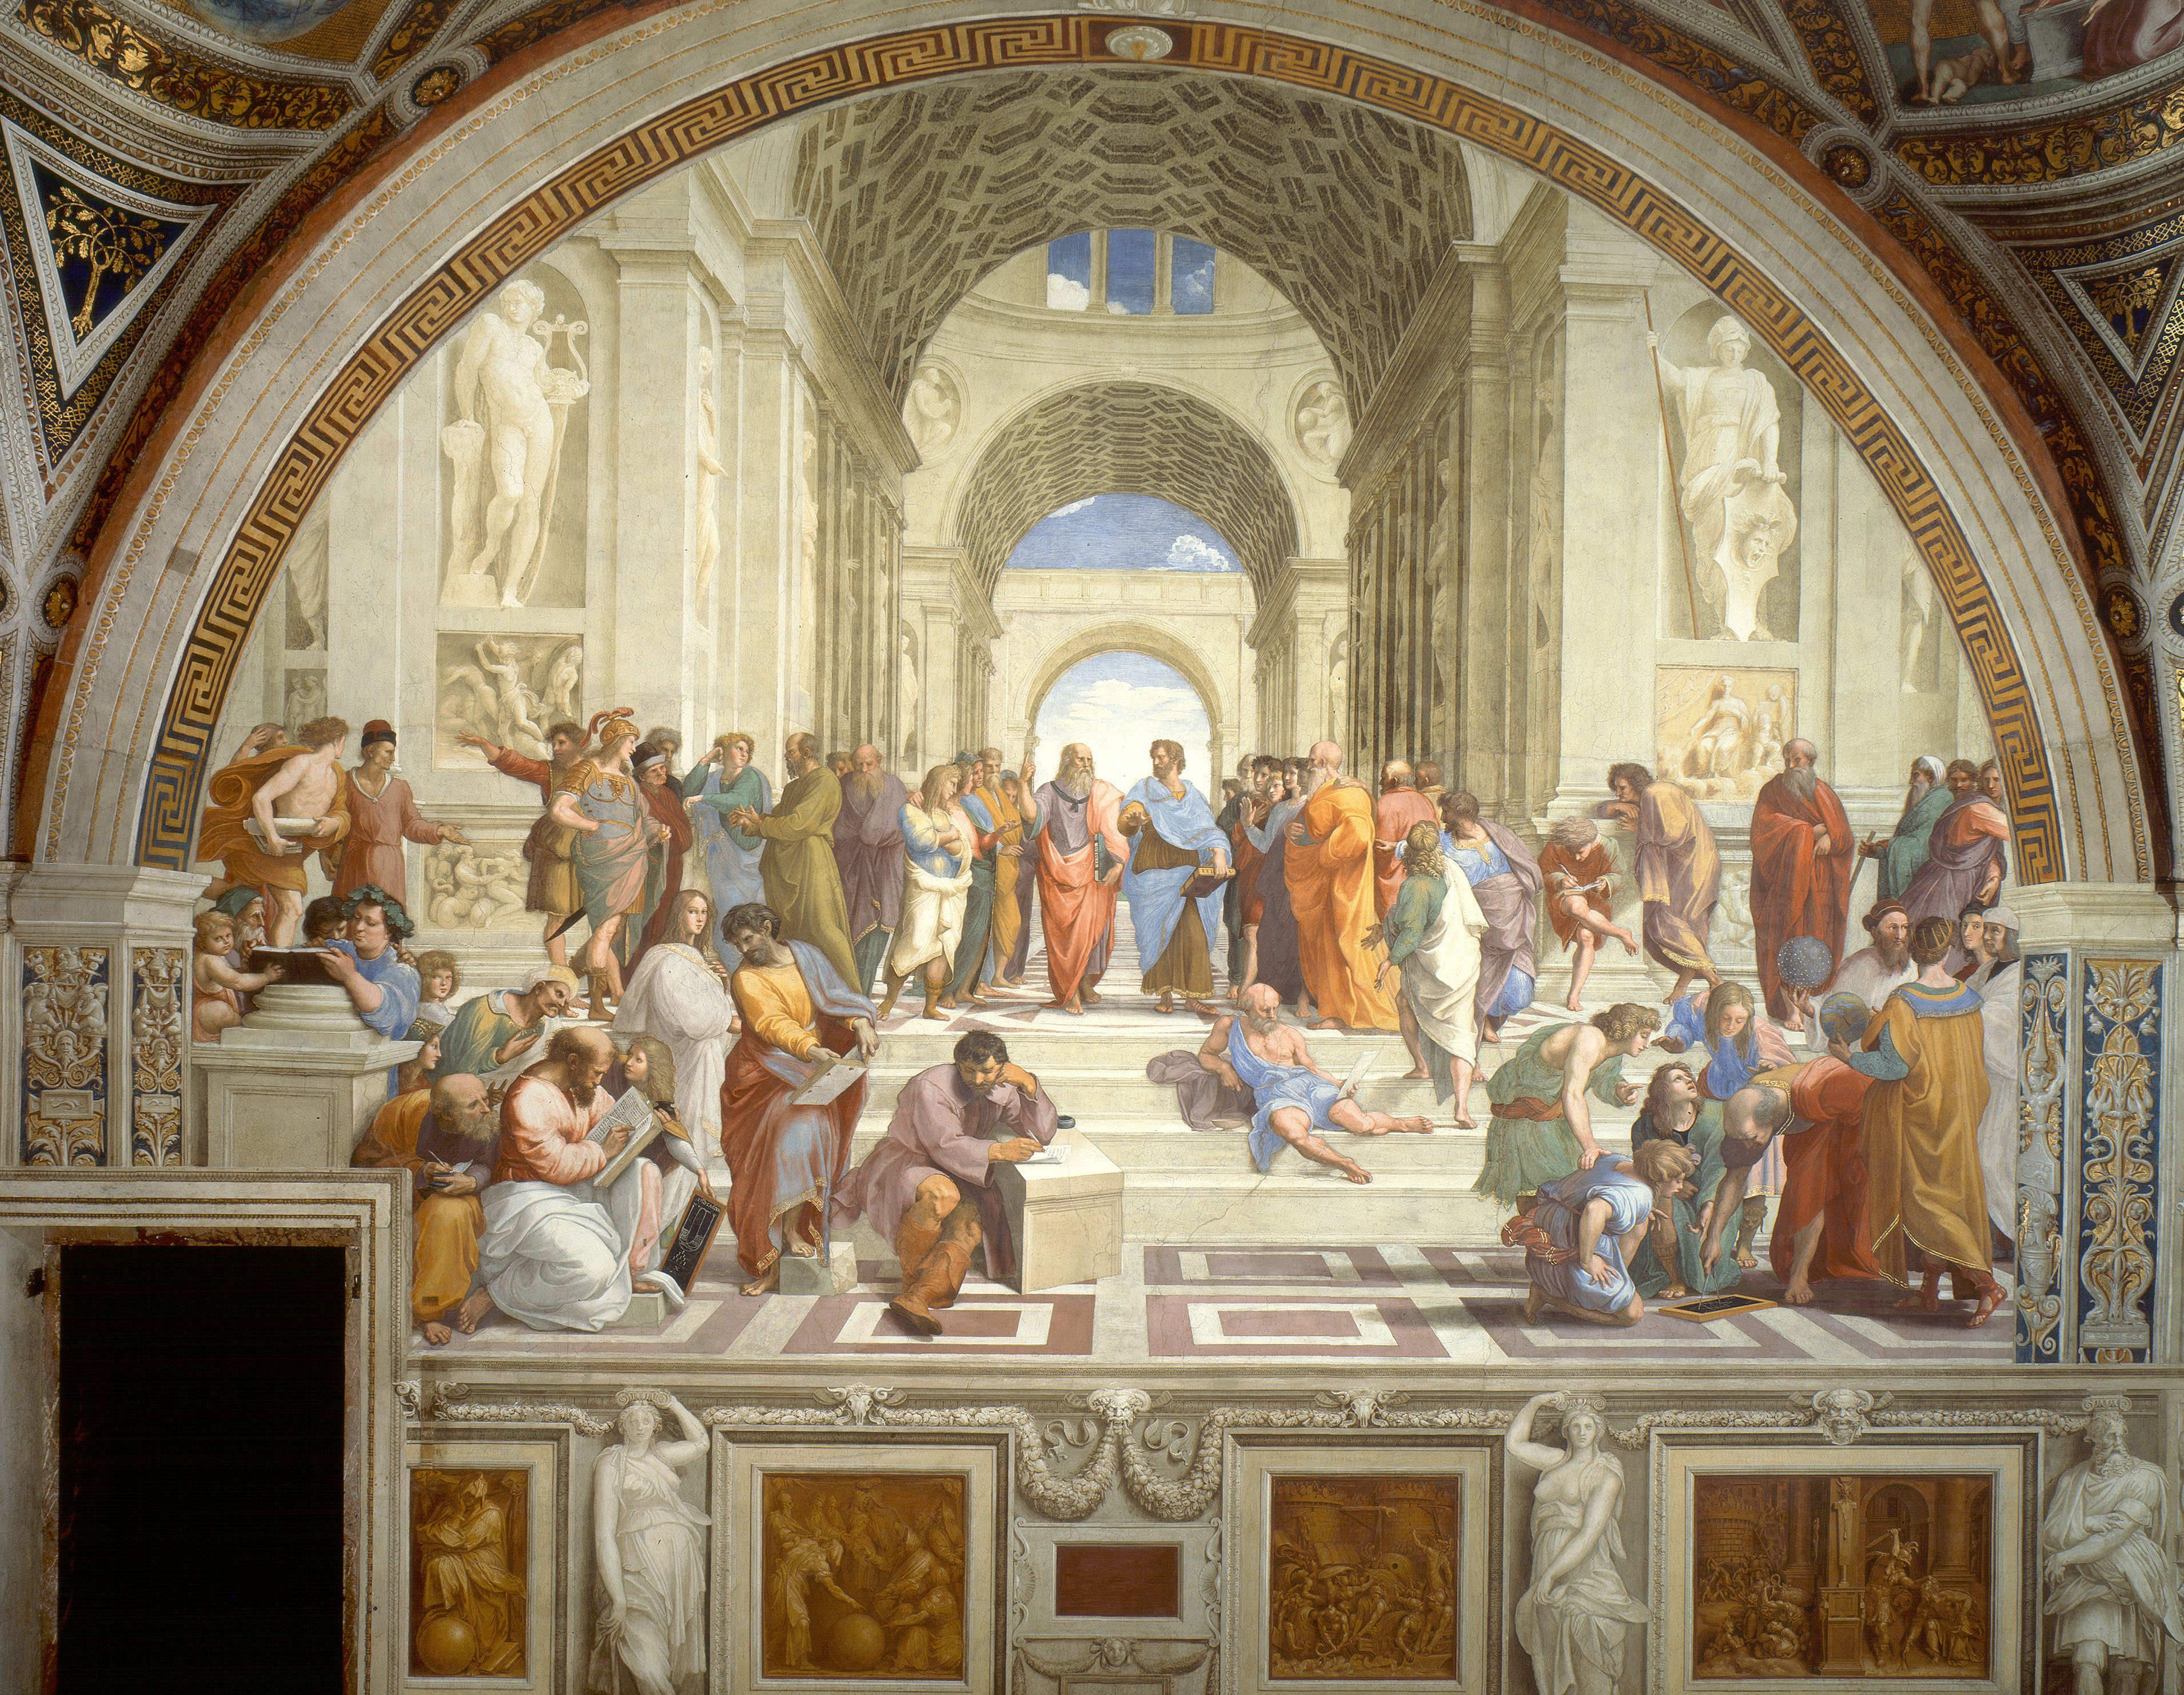
\includegraphics[scale=2]{./imagens/scuola_di_atene.jpeg}}}

\begin{flushright}
	\vspace*{3cm}
	\fontsize{50pt}{20pt}\sffamily\selectfont\textbf{\color{white} ELEMENTOS DE MATEMÁTICA}\\

\vfill

	\Huge\textbf{\color{white} \autor}
\end{flushright}

\restoregeometry

\cleardoublepage

\frontmatter % (Numera as páginas com algarismos romanos.)

% ATENÇÃO SOBRE O LIVRO NÃO ESTAR TERMINADO
\thispagestyle{empty}

\begin{center}
{\Huge \textbf{ATENÇÃO}\\
ESTE LIVRO NÃO ESTÁ TERMINADO.\\
O PROJETO AINDA ESTÁ EM EXECUÇÃO E NÃO HÁ DATA PREVISTA PARA TÉRMINO.}
\end{center}


% Páginas de Rosto e Informações de Citação e Licença
\newgeometry{
	hmargin={2.5cm,2.5cm}, % Margens esquerda (dentro) e direita (fora)
	vmargin={3cm,1cm} % Margens superior e inferior
}

\thispagestyle{empty}

\begin{flushleft}
	\vspace*{2cm}
	\Huge\textbf{\titulo}
\end{flushleft}

\cleardoublepage

\thispagestyle{empty}

\begin{flushleft}
	\Large \autor
	\vspace{2cm}\\
	\Huge\textbf{\titulo}
	\vspace{0.5cm}\\
	\Large\subtitulo
\end{flushleft}

	\vfill

\begin{figure}[!h]
	\centering
	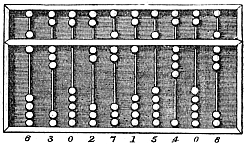
\includegraphics[scale=0.5]{./imagens/abacus}
%	\caption*{\scshape Livros \& Liberdade}
	\caption*{\scshape Livros Livres}
	% Ideias de nomes de editora: Publicações Livres Campinas, Teoria Livre, Conhecimento Livre, Saber Livre, Livro Livre, Liber Libera/Libera Liber (Livro Livre em Latim, precisa conferir se é assim mesmo), Livr\oe, Liber \& Libertatem.
\end{figure}

\clearpage

\restoregeometry
\thispagestyle{empty}

\noindent
\autor \\
\href{mailto:\ecorreio{}}{\texttt{\ecorreio{}}}\\
Campinas, SP, Brasil

\vfill

\noindent Arte da capa: \textit{Scuola di Atene} (1511), Raffaello Sanzio.
\vspace*{0.5cm}\\
Versão \versao. Última revisão em \today.
\vspace*{0.5cm}\\
\begin{small}
\noindent
\ccLogo{} Licença Creative Commons (CC BY-SA 4.0).\\
Este livro pode ser compartilhado e redistribuído em qualquer suporte ou formato, adaptado, transformado e reeditado sob as seguintes condições.\\
Atribuição --- Você deve dar o crédito apropriado, prover um link para a licença e indicar se mudanças foram feitas. Você deve fazê-lo em qualquer circunstância razoável, mas de maneira alguma que sugira ao licenciante a apoiar você ou o seu uso.\\
Compartilha Igual --- Se você reorganizar, transformar ou criar a partir do material, tem de distribuir as suas contribuições sob a mesma licença que o original.\\
Sem restrições adicionais --- Você não pode aplicar termos jurídicos ou medidas de caráter tecnológico que restrinjam legalmente outros de fazerem algo que a licença permita.\\
Para mais informações sobre a licença acesse:\\
\url{https://creativecommons.org/licenses/by-sa/4.0/deed.pt_BR} ou\\
\url{https://wiki.creativecommons.org/wiki/Brazil}. \hfill

\includegraphics[height=\baselineskip]{./imagens/licenca.png}
\end{small}


% Sumário, Lista de Figuras e Lista de Tabelas
\tableofcontents
%\listoffigures
%\listoftables

\cleardoublepage

\phantomsection
\addcontentsline{toc}{chapter}{Prefácio}
\chapter*{Prefácio}

Este projeto nasceu de algumas notas de aula pessoais durante um curso de graduação a que assisti no segundo semestre de 2016. O nome do curso era \textit{Anéis e Corpos} e o contato com o formalismo matemático e com os resultados da teoria matemática apresentada, que começou com a definição de um anel e terminou com a demonstração de que não existe solução em radicais de polinômios de grau maior que 4, foram muito estimulantes. Ao mesmo tempo, eu tinha recentemente aprendido a usar o \LaTeX e estava curioso para testar minhas novas técnicas em algum projeto maior. Esses fatores me levaram a começar a digitar.

Eu posso dizer que este projeto é fruto de dois interesses pessoais: um teórico e um estético. O primeiro, certamente, foi minha motivação principal. O interesse por conhecer e descobrir mais matemática é o que me levou a começar este livro. O segundo, no entanto, também teve seu papel. O prazer estético de produzir um livro desde o zero, o que o \LaTeX proporciona a qualquer leigo em diagramação como eu, estimularam-me em vários momentos, inclusive quando o cansaço ou o desinteresse me impediam de progredir com a escrita.

Originalmente, meu objetivo era organizar algumas notas para estudar e compartilhar com colegas de curso. Já então eu pretendia disponibilizar essas notas para os futuros graduandos em matemática, mas os objetivos do projeto ainda não eram tão grandes. Quando comecei a considerar essas ideias \--- escrever um livro e disponibilizá-lo à comunidade \--- fiquei muito animado e, ao longo dos meses seguintes, ampliei rapidamente meus horizontes. Passei da ideia de escrever notas sobre um curso específico ao objetivo (ingenuamente) extenso de escrever sobre toda a matéria da graduação, tirando e pondo uma coisa ou outra. Como era de se esperar, rapidamente percebi que o projeto estava ficando longo demais para se ver um fim próximo.

Muito do livro ainda não está escrito. De fato, quase nada. A falta de tempo me permitiu somente escrever às vezes e, por isso, decidi primeiro digitar um esquema lógico das definições e teoremas para depois completar com comentários, explicações, discussões e dúvidas que tinha na cabeça enquanto o escrevia. Reluto em disponibilizar este material como está principalmente por não querer que ele se trate de uma apostila normativa e seca \--- uma lista de definições, teormeas e demonstrações \--- mas sim querer que se trate de um livro que apresente resultudados teóricos, gere dúvidas relevantes e suscite discussão. Sob certa óptica, esse objetivo pode parecer presunçoso, mas ele é, na verdade, esperançoso.

\vfill

\begin{flushright}
P. G. M.\\
Campinas, 8 de julho de 2017
\end{flushright}

\phantomsection
\addcontentsline{toc}{chapter}{Agradecimentos}
\chapter*{Agradecimentos}

Um livro nunca é o trabalho de uma pessoa só. Este, em particular, não seria possível sem a contribuição, direta ou indireta, consciente ou não, de várias pessoas. No âmbito da edição e diagramação do livro, agradeço \emph{Donald Knuth} pela criação do \TeX  e \emph{Leslie Lamport} pelo \LaTeX. Agradeço a todos envolvidos nos pacotes que utilizei para a edição deste livro. No âmbito do contúdo do livro, agradeço aos meus colegas \emph{Fábio Meneghetti}, \emph{Pedro Caetano}, \emph{Caio Laurenti}, \emph{Augusto Pereira} e \emph{Matheus Manzatto} pelas proveitosas discussões matemáticas e aos professores que sempre me instigaram pela minha vida de escola e universidade.
\phantomsection
\addcontentsline{toc}{chapter}{Introdução}
\chapter*{Introdução}

Este livro trata de teoria matemática básica e foi escrito para que pudesse ser lidos de dois modos que eu acredito serem complementares. Como é costume em qualquer texto matemático teórico, as definições, proposições e demonstrações são destacadas em ambientes específicos dentro do texto. Entre esses ambientes está a discussão de aspectos relevantes a respeito de cada uma das definições, proposições e demonstrações. No entanto, o leitor interessado somente no encadeamento lógico da teoria pode seguir somente pelos ambientes destacados sem preocupação.

O conteúdo do livro está dividido em três partes. A primeira desenvolve aspectos básicos da teoria de Conjuntos e das teorias de funções e relações. Além disso, são discutidas construções de conjuntos numéricos, que serão importantes como modelos mais gerais estudados à frente. A segunda trata das bases da Álgebra, focando principalmente nas estruturas algébricas mais importante: grupos, anéis, corpos e espaços vetoriais. A terceira parte diz respeito à Topologia e à Geometria, tanto num aspecto amplo da topologia geral como da topologia dos espaços métricos, e preparam para o estudo de espaços reais e da análise em geral, em que são discutidas apresentadas as teorias de diferenciação, integração e medida.
%\include{logica}

% ELEMENTOS TEXTUAIS
%---------------------------------------------------------------------------------------------------------------------------
\mainmatter % (Numera as páginas com algarismos arábicos.)

% Partes
\part{{\scshape Conjuntos}}

\chapter{Os Axiomas e as Contruções Essenciais}

\subsection*{Conjunto, Pertencimento e os Símbolos da Lógica Formal}

A noção de um \emph{conjunto} é uma noção primitiva na matemática. Intuitivamente, um conjunto é um objeto que tem \emph{elementos}. Cada elemento tem para com o conjunto em que está a relação de \emph{pertencimento}. Abstraindo mais essa noção, pensamos que todas as propriedades de um conjunto se resumem aos elementos que a ele pertencem, de modo que um conjunto é, de fato, seus elementos. A \emph{Teoria de Conjuntos} é uma teoria da lógica formal que procura formalizar essas ideias e estudar suas consequências. Neste livro, o tratamento da teoria de conjuntos será um tratamento informal, embora muita ênfase seja dada nos axiomas que constituem uma base para a teoria de conjuntos.

A lógica formal estuda sentenças formadas a partir de símbolos pré-determinados e fixos e as regras que dizem como essas sentenças se relacionam para formar novas sentenças. No tratamento formal da teoria de conjuntos, não há distinção entre conjunto e elemento. Ambos são somente denotados por letras de um alfabeto específico, e a relação de pertencimento é geralmente denotada pelo o símbolo $\in$. Se $X$ e $Y$ são conjuntos, a sentença ``o conjunto $X$ pertence ao conjunto $Y$'' ou ``o conjunto $X$ é elemento do conjunto $Y$'' é denotada por 
	\begin{equation*}
	X \in Y.
	\end{equation*}
Para afirmar que um conjunto $X$ não é elemento de um conjunto $Y$, ou seja, negar $X \in Y$, o símbolo usado é $\notin$ e se denota $X \notin Y$.

As teorias da lógica formal costumam ter axiomas, sentenças assumidas válidas a partir das quais deve-se inferir todas as outras sentenças da teoria. Axiomas, neste livro, serão enunciados, não como sentenças simbólicas, mas como sentenças em português. No entanto, alguns símbolos lógicos frequentemente facilitam e deixam mais claros os enunciados de sentenças na matemática. Os símbolos
	\begin{equation*}
	\forall \qquad \exists
	\end{equation*}
serão usados para substituirem as expressões ``para todo'' e ``existe'', respectivamente (desconsiderando possíveis flexões gramaticais). Eles indicam que alguma propriedade vale para todo elemento de um conjunto ou que existem elementos do conjunto para o qual a propriedade vale. O símbolo $\exists!$ significa que existe e é único e o símbolo $\nexists$ que não existe. Além desses, serão usados também os símbolos
	\begin{equation*}
	\entao \se \sse
	\end{equation*}
para significar a implicação material em cada sentido e a equivalência lógica. Por fim, para os conectivos `e' e `ou'  são usados os símbolos
	\begin{equation*}
	\e \qquad \ou
	\end{equation*}
Esse conectivos indicam, informalmente, que sentenças são ambas verdadeiras, no caso de `e', ou ao menos uma das duas é, no caso de `ou'. Os parênteses, que são comumente usados na lógica formal, serao substituidos por espaços, de modo que não haja ambiguidade. Mais detalhes sobre lógica formal e o uso dos símbolos lógicos serão suprimidos. Para aprofundamento em lógica e sistemas dedutivos, um livro indicado é \emph{Introduction to Logic}, de Alfred Tarski.

\section{Axiomas do Vazio, da Extensão e das Partes}

Os conceitos definidos nesta seção são \emph{igualdade} e \emph{contenção} de conjuntos. O primeiro axioma a ser considerado é o que define que existe um conjunto sem nenhum elemento, o \emph{conjunto vazio}. Esse conjunto tem um papel semelhante ao número zero. Ele é, de certo modo, um ``objeto neutro'' na teoria de conjuntos. Ao decorrer do desenvolvimento da teoria, essa frase sem significado matemática de fato ganhará um significado intuitivo e, em vários casos, uma definição mais precisa.

\begin{axi}[Vazio]
Existe o \emph{conjunto vazio}, um conjunto que não possui elementos. Denota-se esse conjunto por $\emptyset$.
\end{axi}

Formalmente, o axioma é $\exists x \forall y(y \notin x)$  e um conjunto vazio é um conjunto $x$ que satisfaz $\forall y(y \notin x)$. Como o conjunto vazio não possui elementos, sempre que se conclui que existe um elemento em $\emptyset$, ou seja, que existe $x \in \emptyset$, chega-se em uma contradição e a conclusão é que o que se assumiu para chegar na contradição é falso. Essa é uma forma padrão de se demonstrarem diversas proposições na lógica e na matemática.

O segundo axioma considerado é um axioma baseado em uma dos primeiras propriedades de um conjunto quando pensado intuitivamente: a ideia de que, quando abtrai-se da realidade, um conjunto é totalmente definido pelos elementos a que ele pertencem. Esse axioma se chama axioma da extensão e é a definição de \emph{igualdade} entre conjuntos.

\begin{axi}[Extensão]
Sejam $X$ e $Y$ conjuntos. Os conjuntos $X$ e $Y$ são \emph{iguais} se, e somente se, %todo elemento de $X$ pertence a $Y$ e todo elemento de $Y$ pertence a $X$.
	\begin{equation*}
	\forall x \in X \ x \in Y \e \forall y \in Y \ y \in X.
	\end{equation*}
Denota-se $X=Y$. Caso contrário, denota-se $X \neq Y$.
\end{axi}

Formalmente, o axioma é $\forall x \forall y (x = y \leftrightarrow \forall z (z \in x \leftrightarrow z \in y))$.  Quando se consideram conjuntos, é muito útil falar apenas de alguns de seus elementos, um conjunto desses elementos, possivelmente com alguma propriedade específica. Essa noção é a de um subconjunto, um conjunto cujos elementos pertencem todos a um outro conjunto considerado anteriormente. A definição de um subconjunto pode ser dada simplesmente a partir das noções primitivas já fornecidas, pois na ideia de subconjunto só são necessárias as noções de conunto e pertencimento, além dos símbolos lógicos.

\begin{defi}
Seja $X$ um conjunto. Um \emph{subconjunto} (ou uma \emph{parte}) de $X$ é um conjunto $Y$ que satisfaz
	\begin{equation*}
	\forall y \in Y \quad y \in X.
	\end{equation*}
Denota-se $Y \subseteq X$. Caso contrário, denota-se $Y \nsubseteq X$. Um subconjunto \emph{próprio} de $X$ é um subconjunto $Y \subseteq X$ tal que $Y \neq X$. Denota-se $Y \subset X$.
\end{defi}

Formalmente, a definição é $\forall x \forall y (x \subseteq y \leftrightarrow \forall z (z \in x \rightarrow z \in y))$. 

\begin{prop}
Seja $X$ um conjunto. Então
	\begin{enumerate}
	\item $\emptyset \subseteq X$;
	\item $X \subseteq \emptyset \entao X=\emptyset$.
	\end{enumerate}
\end{prop}
\begin{proof}
Suponha que $\emptyset$ não é subconjunto de $X$. Então existe $e \in \emptyset$ tal que $e \notin X$. Mas $e \in \emptyset$ é um absurdo, o que mostra que $\emptyset \subseteq X$.
\end{proof}

O próximo axioma considerado é o que garante que os subconjuntos de um conjunto dado formam um conjunto.

\begin{axi}[Partes]
Seja $X$ um conjunto. Então existe o \emph{conjunto das partes} de $X$, o conjunto que contém todos os subconjuntos de $X$. Denota-se $\p(X)$.
\end{axi}

\begin{prop}
Sejam $X$ e $Y$ conjuntos. Então
	\begin{equation*}
	X \subseteq Y \entao \p(X) \subseteq \p(Y).
	\end{equation*}
\end{prop}

\section{Axiomas da Especificação e do Par}

A noção intuitiva de subconjunto está diretamente relacionada à ideia de formar, a partir de um conjunto e uma propriedade, o subconjunto dos elementos que têm essa propriedade. A existência desse subconjunto é um axioma, chamado axioma da especificação porque a propriedade dada é um especificação dos elementos do conjunto original.

\begin{axi}[Especificação]
Sejam $X$ um conjunto e $\phi(x)$ uma sentença lógica. Existe o conjunto dos elementos de $X$ que satisfazem $\phi(x)$. Denota-se
	\begin{equation*}
	\set{x \in X}{\phi(x)}.
	\end{equation*}
\end{axi}

O próximo axioma garante, a partir da existência de dois, a existência de um novo conjunto cujos elementos são os dois conjuntos iniciais. Esse é o axioma do par. Embora a princípio sua necessidade não seja óbvia, esse axioma é importante --- ao menos útil --- para o desenvolvimento da teoria de conjuntos.

\begin{axi}[Par]
Sejam $X$ e $Y$ conjuntos. Existe o \emph{par} de $X$ e $Y$, o conjunto que tem como únicos elementos $X$ e $Y$. Denota-se $\{X,Y\}$.
\end{axi}

A partir do axioma do par pode-se formar o conjunto que tem como único elemento um  conjunto $X$ formando o par de $X$ e $X$. Esse conjunto é o conjunto unitário com único elemento $X$.

\begin{defi}
Seja $X$ um conjunto. O \emph{conjunto unitário} de elemento $X$ é o conjunto $\{X,X\}$. Denota-se $\{X\}$.
\end{defi}

\section{Axioma da União}

Nesta seção são apresentadas duas das contruções mais importantes da teoria de conjutos: a união e a interseção. A união de um conjunto de conjuntos denotado $C$ é o conjunto cujos elementos pertencem a algum conjunto que pertence $C$. O axioma da união afirma que esse conjunto existe.

\begin{axi}[União]
Seja $C$ um conjunto. Existe a \emph{união} de $C$, o conjunto dos elementos que pertencem a algum elemento de $C$. Denota-se $\bigcup C$. A união de um par $\{X,Y\}$ é denotada $X \cup Y$.
\end{axi}

Pode-se denotar a conjunto $\bigcup C$ por $\set{x}{\exists X \in C \quad x \in X}$.

\begin{prop} Sejam $X$ e $Y$ conjuntos. Então
	\begin{enumerate}
	\item $\bigcup \emptyset = \emptyset$;
	\item $X \subseteq Y \entao \bigcup X \subseteq \bigcup Y$.
	\end{enumerate}
\end{prop}
\begin{proof}
	\begin{enumerate}
	\item Suponha que $x \in \bigcup \emptyset$. Então $\exists X \in \emptyset$ tal que $x \in X$, o que é absurdo porque não pode existir $X \in \emptyset$.
	
	\item Seja $x \in \bigcup X$. Então existe $C \in X$ tal que $x \in C$. Como $X \subseteq Y$, segue que $C \in Y$, portanto $x \in \bigcup Y$.
	\end{enumerate}
\end{proof}

A interseção de um conjunto não vazio de conjuntos denotado $C$ é o conjunto cujos elementos pertencem a todos conjuntos que pertencem $C$. O conjunto interseção existe por consequêcia do axioma da especificação. Como $C$ é não vazio, basta considerar um conjunto $X \in C$ e a sentença lógica dada por
	\begin{equation*}
	\forall Y \in C \quad x \in Y.
	\end{equation*}
Desse modo, o conjunto interseção é $\set{x \in X}{\forall Y \in C \quad x \in Y}$.

\begin{defi}
Seja $C$ um conjunto não vazio. A \emph{interseção} de $C$ é o conjunto dos elementos que pertecem a todos elementos de $C$. Denota-se $\bigcap C$. A interseção de um par $\{X,Y\}$ é denotada $X \cap Y$.
\end{defi}

Pode-se denotar a conjunto $\bigcap C$ por $\set{x}{\forall X \in C \quad x \in X}$.

\begin{prop}
Seja $C$ um conjunto não vazio. Então
	\begin{equation*}
	\forall X \in C \qquad \bigcap C \subseteq X \subseteq \bigcup C.
	\end{equation*}
\end{prop}

\section{Axioma da Escolha}

Para que o axioma da escolha seja compreensível, deve-se definir alguns conceitos antes. Essencialmente, o axioma da escolha é sobre produto de conjuntos e sobre funções. O nome escolha, de fato, vem de uma função, a função escolha. Para definir o conceito de função, é necessário primeiro definir o que é um par ordenado de elementos de dois conjuntos e o que é o conjunto de pares ordenados desses conjunto, que é chamado produto dos conjuntos. A partir desse produto de dois conjuntos, definem-se função e, a partir de função, define-se o produto de qualquer conjunto.

\subsection*{Pares Ordenados, Produto de Par e Função}

\begin{defi}
Sejam $X$ e $Y$ conjuntos. O \emph{par ordenado} com \emph{primeira coordenada} $X$ e \emph{segunda coordenada} $Y$ é o conjunto
	\begin{equation*}
	(X,Y) \coloneqq \{\{X\},\{X,Y\}\} \in \p\left(\p\left(X \cup Y\right)\right).
	\end{equation*}
\end{defi}

\begin{prop}
Sejam $X,Y,Z$ e $W$ conjuntos. Então
	\begin{equation*}
	(X,Y) = (Z,W) \sse X=Z \e Y=W.
	\end{equation*}
\end{prop}

\begin{defi}
Sejam $X$ e $Y$ conjuntos. O \emph{produto} de $X$ por $Y$ é o conjunto
	\begin{equation*}
	X \times Y \coloneqq \set{(x,y) \in \p\left(\p\left(X \cup Y\right)\right)}{x \in X \e y \in Y}.
	\end{equation*}
\end{defi}

A existência desse conjunto depende da união de pares, do conjunto das partes e do axioma de especificação.

%\begin{defi}[Ênupla Ordenada]
%	Sejam $A$ e $B$ conjuntos. O \emph{par (ordenado)} dos elementos $a \in A$ e $b %\in B$ é o conjunto
%	\begin{equation*}
%	(a,b) \coloneqq \{\{a\},\{a,b\}\}.
%	\end{equation*}
%De modo mais geral, sejam $A_1, \ldots, A_n$ $n$ conjuntos e $I \coloneqq \{1,\ldots,n\}$. A \emph{n-upla (ordenada)} dos elementos $a_i \in A_i$, para todo $i \in I$, é definida indutivamente por
%	\begin{equation*}
%	(a_1,\ldots,a_n) \coloneqq ((a_1,\ldots,a_{n-1}),a_n)	
%	\end{equation*}
%\end{defi}
%
%Assim, uma \emph{tripla} é
%	\begin{equation*}
%	(a,b,c) = ((a,b),c)=\{\{(a,b)\},\{(a,b),c\}\}=\{\{\{\{a\},\{a,b\}\}\},\{\{\{a\},\{a,b\}\},c\}\},
%	\end{equation*}
%claramente uma confusão desnecessária se não escrevermos $(a,b,c)$.

%\begin{prop}
%	Seja $A$ um conjunto não vazio. Então, para todos $a,b \in A$, vale $(a,b)=(b,a) \Leftrightarrow a=b$.
%\end{prop}
%\begin{proof}
%	Suponha $(a,b)=(b,a)$. Então $\{\{a\},b\}=\{\{b\},a\}$. Mas então $\{a\} \in (b,a)$, o que implica $\{a\}=\{b\}$ ou $\{a\}=a$. O primeiro caso implica $a=b$. O segundo caso é claramente impossível, pois nenhum conjunto pode ter como único elemento ele mesmo. A implicação contrária é trivial.
%\end{proof}
%
%\begin{prop}
%	Sejam $A_1,\ldots,A_n$ $n$ conjuntos não vazios. Então, para todos $a_i,b_i \in A_i$, $i \in \{1,\ldots,n\}$, vale
%	\begin{equation*}
%	(a_1,\ldots,a_n)=(b_1,\ldots,b_n) \Leftrightarrow a_i=b_i \quad \forall i \in \{1,\ldots,n\}.
%	\end{equation*}
%\end{prop}

\begin{defi}
Sejam $X$ e $Y$ conjuntos. Uma \emph{função} de $X$ para $Y$ é um conjunto $f \subseteq X \times Y$ que satisfaz
	\begin{equation*}
	\forall x \in X \ \exists! y \in Y \qquad (x,y) \in f.
	\end{equation*}
Esse $y$ é a \emph{imagem} de $x$, denotada por $f(x)$. Denotam-se $f: X \to Y$ e $f(x) \coloneqq y$. Para qualquer conjunto $K \subseteq X$, defini-se a \emph{imagem} de $K$
	\begin{equation*}
	f(K)=\set{y \in Y}{\exists k \in K \quad y=f(k)},
	\end{equation*}
que é subconjunto de $Y$. Diz-se que o conjunto $f(X)$ é a \emph{imagem} de $f$.
\end{defi}

\begin{prop}
	Seja $f: A \to B$.
	\begin{enumerate}
	\item $A=\emptyset \sse f=\emptyset$.
	\item $B=\emptyset \entao A=\emptyset$.
	\end{enumerate}
\end{prop}
\begin{proof}
	\begin{enumerate}
	\item Suponhamos que $A=\emptyset$. Primeiro, notemos que $f=\emptyset$ é uma função de $\emptyset$ em $B$. Claramente, $f = \emptyset \subseteq \emptyset \times B$. Ainda, se $f$ não fosse função de $\emptyset$ em $B$, existiria $a \in \emptyset$ tal que não existe único $b \in B$ satisfazendo $(a,b) \in f$. Mas existir $a \in \emptyset$ é um absurdo. Logo $f$ é função. Por fim, se $g: \emptyset \times B$ é uma função, como $\emptyset \times B = \emptyset$, então $g \subseteq \emptyset \times B = \emptyset$, logo $g=\emptyset=f$.
	
	Reciprocamente, suponhamos $f=\emptyset$. Se $A \neq \emptyset$, seja $a \in A$. Como $f$ é função, existe $b \in B$ tal que $(a,b) \in f=\emptyset$, o que é absurdo. Portanto $A=\emptyset$.
	
	\item Suponhamos que $A \neq \emptyset$. Então existe $a \in A$ e, como $f$ é função, existe único $b \in \emptyset$ tal que $(a,b) \in f$. Mas $b \in \emptyset$ é absurdo, o que mostra que $A = \emptyset$.
	\end{enumerate}
\end{proof}

\subsection*{O Axioma da Escolha e Produto de Conjuntos}

\begin{defi}
Seja $C$ um conjunto. O \emph{produto} de $C$ é o conjunto
	\begin{equation*}
	\prod C \coloneqq \set{f: C \to \bigcup C }{\forall X \in C \quad f(X) \in X}.
	\end{equation*}
	\begin{equation*}
	\prod C \coloneqq \set{f \in \left(\bigcup C\right)^C }{\forall X \in C \quad f(X) \in X}.
	\end{equation*}
\end{defi}

\begin{prop}
Seja $C$ um conjunto. Então
	\begin{enumerate}
	\item $C = \emptyset \entao \prod C = \{\emptyset\}$;
	\item $\emptyset \in C \entao \prod C = \emptyset$.
	\end{enumerate}
\end{prop}
\begin{proof}
	\begin{enumerate}
	\item Como $C=\emptyset$, então $\bigcup \emptyset = \emptyset$. A função $\emptyset: \emptyset \to \emptyset$ é uma função em $\prod C$, pois satisfaz por vacuidade que $\forall X \in C \quad f(X) \in X$. Se não satisfizesse, existiria $X \in \emptyset$ tal que $f(X) \notin X$, o que é contradição. Isso mostra que $\emptyset \in \prod \emptyset$. Agora, seja $f \in \prod \emptyset$ função de $\emptyset$ em $\emptyset$. Como o domínio de $f$ é $\emptyset$, segue que $f=\emptyset$.
	
	\item Suponha que existe $f \in \prod C$. Então $f: C \to \bigcup C$ satisfaz que $\forall X \in C \quad f(X) \in X$. Como $\emptyset \in C$, existe $f(\emptyset) \in \bigcup C$ e, pela propriedade, $f(\emptyset) \in \emptyset$, contradição. Portanto $\prod C = \emptyset$.
	\end{enumerate}
\end{proof}

\begin{axi}[Escolha]
Seja $C$ um conjunto tal que $\emptyset \notin C$. Então $\prod C \neq \emptyset$.
\end{axi}



\section{Axiomas do Infinito e da Fundação}

\begin{defi}
Seja $X$ um conjunto. O \emph{sucessor} de $X$ é o conjunto
	\begin{equation*}
	X^+ \coloneqq X \cup \{X\}.
	\end{equation*}
\end{defi}

\begin{axi}
Existe um \emph{conjunto indutivo}, um conjunto que contém $\emptyset$ e contém o sucessor de cada um de seus elementos.
\end{axi}

\begin{prop}
Seja $I$ um conjunto indutivo e $C$ o conjunto dos subconjuntos de $I$ que são indutivos. Então $\bigcap C$ é um conjunto indutivo.
\end{prop}

\section{Axioma da Substituição}

Os axiomas da especificação e do par são consequência do axioma da substituição.


\section*{Propriedades Gerais}

\subsection*{Contenção}

\begin{prop}
Sejam $X$, $Y$ e $Z$ conjuntos. Então
	\begin{enumerate}
	\item $X \subseteq X$;
	\item $X \subseteq Y \e Y \subseteq X \sse X=Y$;
	\item $X \subseteq Y \e Y \subseteq Z \entao X \subseteq Z$.
	\end{enumerate}
\end{prop}
\begin{proof}
	\begin{enumerate}
	\item Se $X=\emptyset$, então $\emptyset \subseteq X = \emptyset$. Logo $X \subseteq X$. Caso contrário, seja $x \in X$. Então $x \in X$. Logo $X \subseteq X$.
	\item $X \subseteq Y$ e $Y \subseteq X$ se, e somente se, $\forall x \in X \ x \in Y \e \forall y \in Y \ y \in X$, o que é equivalente a $X=Y$ pelo axioma da extensão.
	\item Se $X=\emptyset$, então $X \subseteq Z$. Caso contrário, seja $x \in X$. Então, como $X \subseteq Y$, $x \in Y$ e, como $Y \subseteq Z$, $x \in Z$. Logo $X \subseteq Z$.
	\end{enumerate}
\end{proof}

\subsection*{União e Interseção}

\begin{prop}
Sejam $X$, $Y$ e $Z$ conjuntos. Então
	\begin{enumerate}
	\item $X \cup \emptyset = X$;
	\item $X \cup Y = Y \cup X$;
	\item $(X \cup Y) \cup Z = X \cup (Y \cup Z)$;
	\item $X \cup X = X$;
	\item $X \subseteq Y \sse X \cup Y = Y$.
	\end{enumerate}
\end{prop}

\begin{prop}
Sejam $X,Y$ e $Z$ conjuntos. Então
	\begin{enumerate}
	\item $X \cap \emptyset = \emptyset$;
	\item $X \cap Y = Y \cap X$;
	\item $(X \cap Y) \cap Z = X \cap (Y \cap Z)$;
	\item $X \cap X = X$;
	\item $X \subseteq Y \sse X \cap Y = X$.
	\end{enumerate}
\end{prop}

\begin{prop}
Sejam $X$, $Y$ e $Z$ conjuntos. Então
	\begin{enumerate}
	\item $X \cap (Y \cup Z) = (X \cap Y) \cup (X \cap Z)$;
	\item $X \cup (Y \cap Z) = (X \cup Y) \cap (X \cup Z)$.
	\end{enumerate}
\end{prop}

\chapter{Famílias e Propriedades de Conjuntos}

\section{Famílias e Indexações}

Os axiomas já foram todos enunciados no capítulo anterior e as bases da teoria de conjuntos clássica está construída. Sendo assim, é necessário mudar a linguagem com que muitas das operações sobre conjuntos são tratadas, entre elas a união, a interseção e o produto. O conceito de uma família será definido nesta seção. Embora inicialmente a notação do capítulo anterior seja mais simples, eventualmente a notação de famílias com índices será necessária, por dois motivos principais. O primeiro é que esse conceito facilitará muito os enunciados de várias propriedades e teoremas na matemática eventualmente. O segundo é que tradicionalmente os matemáticos usam famílias e índices para denotar uniões, interseções, produtos e muitas outras noções. A ideia básica de uma família é a seguinte. Quando se define a união de um conjunto $C$ na teoria de conjuntos, a ideia intuitiva por trás da definição é que se estão unindo os conjuntos que são elementos de $C$. A união de um par $\{X,Y\}$ é denotada $X \cup Y$ não por acaso, essa notação indica um conjunto que está sendo formado com os elementos de $X$ e $Y$, não com os elementos dos elementos de $C$, como no caso de $\bigcup C$. 

Generalizando essa ideia, a união de três conjuntos $X_1,X_2,X_3$ pode ser denotada $X_1 \cup X_2 \cup X_3$ e o mesmo pode ser feito para qualquer quantidade finita de conjuntos. Mas para fazer o mesmo para uma quantidade qualquer de conjuntos, não é possível escrever esses conjuntos numa lista. Por isso surgiu a ideia de \emph{indexar} os conjuntos de $C$ que se pretende unir, usando a notação $(X_i)_{i \in I}$, sendo que cada $X_i$ é um elemento de $C$ e $i$ seu índice. Em seguida, indica-se na parte inferior do símbolo de união que os conjuntos indexados estão sendo unidos, de modo que $\bigcup C$ é denotado
	\begin{equation*}
	\bigcup_{i \in C} X_i.
	\end{equation*}

Essa notação tem a vantagem de estar mais próxima da intuição e também permite trabalhar com duplas uniões mais facilmente. As mesmas ideias são aplicadas para interseções e produtos. No entanto, ainda resta um problema, o problema principal. Tendo  já especificada qual é a notação que pretende-se aplicar, ainda falta definir o que é uma família somente a partir dos conceitos da teoria de conjuntos. Essa definição vem a seguir.

\begin{defi}
	Sejam $C$ e $I$ conjuntos não vazios. Uma \emph{família} de elementos de $X$ indexados por $I$ é uma função $F: I \to C$. O conjunto $I$ é o \emph{conjunto de índices} da família. Denota-se isso por
	\begin{equation*}
	(F_i)_{i \in I} \subseteq C
	\end{equation*}
e a imagem de $i \in I$ por $F$ é denotada $F_i$ e chamada de \emph{$i$-ésimo membro} da família.
\noindent
Uma \emph{sequência} é uma família em que $I=\N$, e uma \emph{sequência finita} é uma família em que $I \in \N$ (ou seja, $I=\{0,\ldots,n\}$ para algum $n \in \N$, e nesse caso diz-se $n$-sequência).
\end{defi}

Vale notar que uma família é vazia se, e somente se, $I=\emptyset$. Uma família é uma função e, portanto, quando se afirma que uma família, afirma-se que uma função é vazia, ou que é a função vazia. Mas isso ocorre se, e somente se, seu domínio, no caso o conjunto de índices, é vazio.

\begin{defi}
	Seja $X$ um conjunto não vazio. Uma \emph{indexação} de $X$ é uma família bijetiva $(x_i)_{i \in I}$ de elementos de $X$. Nesse caso, $X$ é um conjunto indexado por $I$ e denota-se $X=\{x_i\}_{i \in I}$.
\end{defi}

A noção de uma família é, de fato, mais motivada por notação do que por um conceito teórico, já que uma família é simplesmennte uma função sem nenhuma restrição além disso, e a única diferença entre uma família é uma função é o contexto de utilização. Uma pergunta relevante, ainda, é se todo conjunto pode ser indexado por meio de uma família. Essa pergunta tem uma resposta óbvia e uma não óbvia, e ambas afirmam que sim. A resposta óbvia é que, para se indexar um conjunto $C$ basta considerar a função $F: C \to C$ definida para todo $X \in C$ por $F(X)=X$. Desse modo, essa é uma indexação do conjunto $X$. Mas essa resposta não satisfaz a tradição de indexar um quantidade finita de conjuntos $\{X,Y\}$ com números naturais. A resposta menos óbvia é que todo conjunto pode ser bem ordenado e, dessa forma, existe uma função de um número ordinal para o conjunto, logo uma indexação desse conjunto por um número ordinal. Os números naturais são os números ordinais finitos, o que significa que essa resposta menos óbvia condiz com a idexação que se faz usualmente de uma quantidade finita de conjuntos. Esse tópicos, no entanto, não serão abordados nesse capítulo.

\section{Propriedades de União e Interseção}

A partir da definição de família, pode-se definir a união e a interseção de uma família de conjuntos a partir da imagem do conjunto de índices $I$ pela função $C$, o conjunto $C(I) = \set{C_i}{i \in I}$. No entanto, um problema teórico se manifesta para se definir uma família de conjuntos. Se uma família é uma função de um conjunto de índices em um conjunto de elementos, para se definir uma família de conjuntos deveria existir um conjunto de todos conjuntos para fazer o papel de contradomínio de uma família. Esse conjunto, no entanto, não existe na teoria de conjuntos abordada neste livro, o que sugere que a definição de uma família de conjuntos depende, de fato, de um conjunto cujos elementos são os conjuntos da família de conjuntos. A existência desse conjunto de conjuntos é suposta, mas ele não é o conjunto de todos os conjuntos. Sendo assim, sempre que se enunciar uma família de conjuntos, essas ressalvas serão assumidas.

\begin{defi}
A \emph{união} de uma família $(C_i)_{i \in I}$ é o conjunto
\end{defi}
	\begin{equation*}
	\bigcup_{i \in I} C_i \coloneqq \bigcup C(I).
	\end{equation*}
A \emph{interseção} de uma família não vazia $(C_i)_{i \in I}$ é o conjunto
	\begin{equation*}
	\bigcap_{i \in I} C_i \coloneqq \bigcap C(I).
	\end{equation*}
\noindent
Quando $I$ for finito, pode-se denotar
	\begin{equation*}
	C_1 \cup \cdots \cup C_n \coloneqq \bigcup_{i \in I} C_i \qquad \e \qquad C_1 \cap \cdots \cap C_n \coloneqq \bigcap_{i \in I} C_i.
	\end{equation*}
	
\begin{prop}
	Seja $(C_i)_{i \in I}$ uma família de conjuntos. Então
	\begin{enumerate}
	\item $\forall i \in I \quad C_i = \emptyset \qquad \Leftrightarrow \qquad \displaystyle \bigcup_{i \in I} C_i = \emptyset$.
	
	\item $\displaystyle \exists i \in I \quad C_i = \emptyset \qquad \Rightarrow \qquad \bigcap_{i \in I} C_i = \emptyset$.
	\end{enumerate}
\end{prop}

\begin{prop}
Seja $(C_i)_{i \in I}$ uma família não vazia de conjuntos. Então
	\begin{enumerate}
	\item $\displaystyle \left( \bigcap_{i \in I} C_i \right)^\complement = \bigcup_{i \in I} (C_i)^\complement$
	
	\item $\displaystyle \left( \bigcup_{i \in I} C_i \right)^\complement = \bigcap_{i \in I} (C_i)^\complement$
	\end{enumerate}
\end{prop}
\begin{proof}
	\begin{enumerate}
	\item Para isso, basta notar que $c \in \left( \bigcap_{i \in I} C_i \right)^\complement$ se, e somente se, $c \notin \bigcap_{i \in I} C_i$. Mas isso ocorre se, e somente se, existe $i \in I$ tal que $c \notin C_i$. Essa afirmação é equivalente a $c \in (C_i)^\complement$ que, por sua vez, é equivalente a $ c \in \bigcup_{i \in I} (C_i)^\complement$.
	
		\item Como, para todo conjunto $C$, $(C^\complement)^\complement = C$, segue do item anterior que
		\begin{equation*}
		\displaystyle \left( \bigcup_{i \in I} C_i \right)^\complement = \left( \bigcup_{i \in I} ((C_i)^\complement)^\complement \right)^\complement = \left( \left( \bigcap_{i \in I} (C_i)^\complement \right)^\complement \right)^\complement = \bigcap_{i \in I} (C_i)^\complement.
		\end{equation*}
	\end{enumerate}
\end{proof}

\begin{prop}
Seja $(C_{ij})$ uma família não vazia de conjuntos. Então
	\begin{equation*}
	\bigcup_{i \in I} \left( \bigcap_{j \in J} C_{ij} \right) \subseteq \bigcap_{j \in J} \left( \bigcup_{i \in I} C_{ij} \right)
	\end{equation*}
\end{prop}

\begin{prop}
Seja $(C_{ij})$ uma família não vazia de conjuntos. Então
	\begin{enumerate}
	\item $\displaystyle\bigcap_{i \in I} \p\left(C_i \right) = \p\left(\displaystyle\bigcap_{i \in I} C_i \right)$;
	\item $\displaystyle\bigcup_{i \in I} \p\left(C_i \right) \subseteq \p\left(\displaystyle\bigcup_{i \in I} C_i \right)$.
	\end{enumerate}
\end{prop}




\cleardoublepage
\section{Produto de Conjuntos}

   \begin{defi}
Seja $(C_i)_{i \in I}$ uma família de conjuntos. O \emph{produto} de $(C_i)_{i \in I}$ é o conjunto
	\begin{equation*}
	\prod_{i \in I} C_i \coloneqq \set{(c_i)_{i \in I}}{\forall i \in I \quad c_i \in C_i}.
	\end{equation*}
As famílias $(c_i)_{i \in I}$ são de elementos em $\bigcup_{i \in I} C_i$.
\end{defi}

\begin{defi}
Seja $(C_i)_{i \in I}$ uma família de conjuntos e $i \in I$. A \emph{projeção canônica} de $\prod_{i \in I} C_i$ em $C_i$ é a função
	\begin{align*}
	\pi_i: \prod_{i \in I} C_i &\to C_i \\
			(c_i)_{i \in I} &\mapsto c_i.
	\end{align*}
\end{defi}

\begin{prop}[Propriedade Universal]
Sejam $(C_i)_{i \in I}$ uma família de conjuntos, $X$ um conjunto e, para todo $i \in I$, $f_i: X \to C_i$ uma função. Então existe única função $f: X \to \prod_{i \in I} C_i$ tal que, para todo $i \in I$, $\pi_i \circ f = f_i$ (o diagrama comuta).
\begin{figure}[!h]
\centering
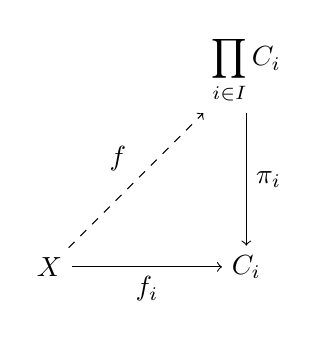
\begin{tikzpicture}[node distance=2.5cm, auto]
	\node (P) {$\displaystyle\prod_{i \in I} C_i$};
	\node (Ci) [below of=P] {$C_i$};
	\node (X) [left of=Ci] {$X$};
	\draw[->] (X) to node [swap] {$f_i$} (Ci);
	\draw[->, dashed] (X) to node {$f$} (P);
	\draw[->] (P) to node {$\pi_i$} (Ci);
\end{tikzpicture}
\end{figure}
\end{prop}
\begin{proof}
Defina a função
	\begin{align*}
	f: X &\to \prod_{i \in I} C_i \\
		x &\mapsto (f_i(x))_{i \in I}.
	\end{align*}
Para todo $x \in X$ e para todo $i \in I$,
	\begin{equation*}
	\pi_i \circ f(x) = \pi_i (f(x)) = \pi_i ((f_i(x))_{i \in I}) = f_i(x).
	\end{equation*}
Portanto $\pi_i \circ f = f_i$. Isso mostra a existência da $f$. Para a unicidade, seja $\overline{f}: X \to \prod_{i \in I} C_i$ função tal que, para todo $i \in I$, $\pi_i \circ \overline{f} = f_i$. Seja $x \in X$.  Como $\overline{f}(x) \in \prod_{i \in I} C_i$, $\overline{f}(x) = (x_i)_{i \in I}$. Da propriedade comutativa de $\overline{f}$, segue que, para todo $i \in I$,
	\begin{equation*}
	x_i = \pi_i \circ \overline{f}(x) = f_i(x).
	\end{equation*}
Como $f(x) = (f_i(x))_{i \in I}$, isso mostra que $\overline{f}(x) = f(x)$. Portanto $\overline{f} = f$.
\end{proof}

\section{Coproduto de Conjuntos}

\begin{defi}
Seja $(C_i)_{i \in I}$ uma família não vazia de conjuntos. O \emph{coproduto} de $(C_i)_{i \in I}$ é o conjunto
	\begin{equation*}
	\coprod_{i \in I} C_i \coloneqq\set{(i,c)}{i \in I \e c \in C_i}.
	\end{equation*}
\end{defi}

\begin{defi}
Seja $(C_i)_{i \in I}$ uma família de conjuntos e $i \in I$. A \emph{inclusão canônica} de $C_i$ em $\coprod_{i \in I} C_i$ é a função
	\begin{align*}
	\iota_i: C_i &\to \coprod_{i \in I} C_i \\
			c &\mapsto (i,c).
	\end{align*}
\end{defi}

\begin{prop}[Propriedade Universal]
Sejam $(C_i)_{i \in I}$ uma família de conjuntos, $X$ um conjunto e, para todo $i \in I$, $f_i: C_i \to X$ uma função. Então existe única função $f: \coprod_{i \in I} C_i \to X$ tal que, para todo $i \in I$, $f \circ \iota_i = f_i$ (o diagrama comuta).
\begin{figure}[!h]
\centering
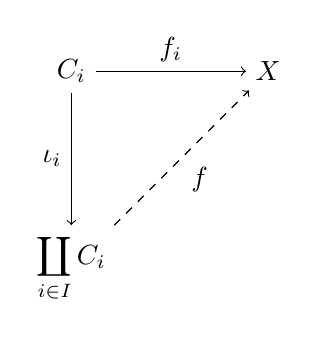
\begin{tikzpicture}[node distance=2.5cm, auto]
	\node (Ci) {$C_i$};
	\node (S) [below of=Ci] {$\displaystyle\coprod_{i \in I} C_i$};
	\node (X) [right of=Ci] {$X$};
	\draw[->] (Ci) to node {$f_i$} (X);
	\draw[->, dashed] (S) to node [swap] {$f$} (X);
	\draw[->] (Ci) to node [swap] {$\iota_i$} (S);
\end{tikzpicture}
\end{figure}
\end{prop}
\begin{proof}
Defina a função
	\begin{align*}
	f: \coprod_{i \in I} C_i &\to X \\
		(i,c) &\mapsto f_i(c).
	\end{align*}
Seja $i \in I$ e $c \in C_i$. Então
	\begin{equation*}
	f \circ \iota_i(c) = f(\iota_i(c)) = f(i,c) = f_i(c).
	\end{equation*}
Portanto $f \circ \iota_i = f_i$. Isso mostra a existência da $f$. Para a unicidade, seja $\overline{f}: \coprod_{i \in I} C_i \to X$ função tal que, para todo $i \in I$, $\overline{f} \circ \iota_i = f_i$. Seja $x \in \coprod_{i \in I} C_i$. Existem $i \in I$ e $c \in C_i$ tais que $x=(i,c)$. Da propriedade comutativa de $\overline{f}$, segue que
	\begin{equation*}
	\overline{f}(x) = \overline{f}(i,c) = \overline{f}(\iota_i(x)) = \overline{f} \circ \iota_i(c) = f_i(c) = f(i,c) = f(x).
	\end{equation*}
Isso mostra que $\overline{f}=f$.
\end{proof}


\cleardoublepage
\begin{figure}
\centering
\begin{tikzpicture}[node distance=4cm, auto]
	\node (P) {$\displaystyle\prod_{i \in I} C_i$};
	\node (Ci) [below of=P] {$C_i$};
	\node (X) [left of=Ci] {$X$};
	\node (S) [below of=Ci] {$\displaystyle\coprod_{i \in I} C_i$};
	\node (Y) [right of=Ci] {$Y$};	
	\draw[->] (X) to node [swap] {$f_i$} (Ci);
	\draw[->, dashed] (X) to node {$f$} (P);
	\draw[->] (P) to node {$\pi_i$} (Ci);
	\draw[->] (Ci) to node {$g_i$} (Y);
	\draw[->, dashed] (S) to node [swap] {$g$} (Y);
	\draw[->] (Ci) to node [swap] {$\iota_i$} (S);
\end{tikzpicture}
\caption*{Os diagramas comutativos do \\produto e do coproduto de conjuntos.}
\end{figure}





\cleardoublepage
\section*{Propriedades Gerais}

%O axioma da escolha reescrito para famílias é o seguinte. Para toda família não vazia $(C_i)_{i \in I}$ de conjuntos (disjuntos) não vazios, existe uma função (\emph{função escolha}) $E: I \to \bigcup_{i \in I} C_i$ tal que, para todo $i \in I$, $E(i) \in C_i$.

%\begin{prop}
%	Seja $(C_i)_{i \in I}$ uma família não vazia de conjuntos. Então
%	\begin{equation*}
%	\prod_{i \in I} C_i = \emptyset \qquad \Leftrightarrow \qquad \exists i \in I \quad C_i = \emptyset.
%	\end{equation*}
%\end{prop}
%\begin{proof}
%	Primeiro, suponhamos que $(C_i)_{i \in I}$ é uma família de conjuntos não vazios. Então, pelo axioma da escolha, existe uma função $E: I \to \bigcup_{i \in I} C_i$ tal que, para todo $i \in I$, $E(i) \in C_i$. Assim, $E \in \prod_{i \in I} C_i$, o que mostra que $\prod_{i \in I} C_i \neq \emptyset$. Reciprocamente, suponhamos que existe alguma $i \in I$ tal que $C_i = \emptyset$. Então, se existisse $c \in \prod_{i \in I} C_i$, seguiria que $c(i) \in C_i = \emptyset$, o que é absurdo. Logo $\prod_{i \in I} C_i = \emptyset$.
%\end{proof}

\begin{prop}
	Seja $(C_{ij})_{(i,j) \in I \times J}$ uma família de conjuntos. Então
	\begin{enumerate}
	\item $\displaystyle \bigcup_{j \in J} \left(\prod_{i \in I} C_{ij}\right) \subseteq \prod_{i \in I} \left(\bigcup_{j \in J} C_{ij}\right)$;
	\item $\displaystyle \bigcap_{j \in J} \left(\prod_{i \in I} C_{ij}\right) = \prod_{i \in I} \left(\bigcap_{j \in J} C_{ij}\right)$.
	\end{enumerate}
\end{prop}
\begin{proof}
	\begin{enumerate}	
	\item \begin{align*}
	c \in \displaystyle \bigcup_{j \in J} \left(\prod_{i \in I} C_{ij}\right) & \Rightarrow \exists j \in J \qquad \qquad c \in \prod_{i \in I} C_{ij} \\
	& \Rightarrow \exists j \in J \ \forall i \in I \qquad c_i \in C_{ij} \\
	& \Rightarrow \forall i \in I \qquad \qquad c \in \bigcup_{j \in J} C_{ij} \\
	& \Rightarrow  c \in \prod_{i \in I} \left(\bigcup_{j \in J} C_{ij}\right).
	\end{align*}
	
	\item 	
	\begin{align*}
	c \in \displaystyle \bigcap_{j \in J} \left(\prod_{i \in I} C_{ij}\right) & \Leftrightarrow \forall j \in J \qquad \qquad c \in \prod_{i \in I} C_{ij} \\
	& \Leftrightarrow \forall j \in J \ \forall i \in I \qquad c_i \in C_{ij} \\
	& \Leftrightarrow \forall i \in I \ \forall j \in J \qquad c_i \in C_{ij} \\
	& \Leftrightarrow \forall i \in I \qquad \qquad c_i \in \bigcup_{j \in J} C_{ij} \\
	& \Leftrightarrow  c \in \prod_{i \in I} \left(\bigcap_{j \in J} C_{ij}\right).
	\end{align*}
	\end{enumerate}
\end{proof}

Notemos que a inclusão contrária no primeiro item nao vale. Suponhamos que para um $j_0 \in J$, todos os $C_{ij_0}$ são vazios, mas para todos outros $j \in J$, os $C_{ij}$ não são vazios. Então o produto desses $C_{ij}$ será sempre vazio, pois sempre tem um dos elementos do produto vazio, e então a união desses produtos será vazia; no entanto, a união desses $C_{ij}$ não será nenhuma vazia e, então, o produto não seráa vazio (pelo axioma da escolha).

\begin{prop}
	Sejam $C_i$ conjuntos 
	
	\begin{equation*}
	f^{-1}\left( \prod_{i \in I} {C_i} \right) = \bigcap f_i^{-1} (C_i).
	\end{equation*}
\end{prop}



%\begin{defi}
%Seja $C$ um conjunto não vazio. A \emph{soma} de $C$ é o conjunto
%	\begin{equation*}
%	\coprod C \coloneqq \set{(X,x) \in C \times \bigcup C}{x \in X}.
%	\end{equation*}
%\end{defi}

%Vale notar que a soma de $C$ existe porque é um subconjunto de $\p\left(C \times \bigcup C \right)$, logo é um conjunto pelo axioma da especificação.

%Definimos a seguir uma nova operação em uma família $(C_i)_{i \in I}$, a soma, também chamada de união disjunta. Em vez de unirmos todos elementos de $(C_i)_{i \in I}$, indexamos cada um deles com o índice do conjunto da família a que ele pertence para que, se um mesmo elemento, digamos $c$, pertencer $C_{i_1}$ e $C_{i_2}$, $i_1,i_2 \in I$ distintos, então na união disjunta $(c,i_1)$ e $(c,i_2)$ serão elementos distintos, enquanto que na união não haverá distinção.



%\begin{conj}
%	Seja $(C_i)_{i \in I}$ uma família não vazia de conjuntos. Então
%	\begin{equation*}
%	\coprod_{i \in I} C_i = \emptyset \qquad \Leftrightarrow \qquad \forall i \in I \quad C_i = \emptyset.
%	\end{equation*}
%\end{conj}


\chapter{Relações e Funções}

\section{Relações}

\begin{defi}
Sejam $X$ e $Y$ conjuntos. Uma \emph{relação} $R$ de $X$ para $Y$ é um subconjunto de $X \times Y$. Os conjuntos $X$ e $Y$ são, respectivamente, o \emph{domínio} e o \emph{contradomínio} de $R$. Denota-se $x \mathrel{R} y$ para $(x,y) \in R$.
\end{defi}

\begin{defi}
Seja $R$ uma relação de $X$ em $Y$. A \emph{relação inversa} de $R$ é a relação $R\inv$ de $Y$ em $X$ definida por
	\begin{equation*}
	\forall x \in X\ \forall y \in Y \qquad x \mathrel{R} y \Leftrightarrow y \mathrel{R\inv} x.
	\end{equation*}
\end{defi}


\section{Funções}

\begin{defi}
Sejam $X$ e $Y$ conjuntos. Uma \emph{função} de $X$ para $Y$ é uma relação $f$ de $X$ para $Y$ que satisfaz
	\begin{equation*}
	\forall x \in X \ \exists! y \in Y \qquad (x,y) \in f.
	\end{equation*}
Esse $y$ é a \emph{imagem} de $x$. Denotam-se $y=f(x)$ e
	\begin{align*}
	f: X &\to Y \\
		x &\mapsto f(y)
	\end{align*}
Para qualquer conjunto $K \subseteq X$, definimos a \emph{imagem} de $K$
	\begin{equation*}
	f(K)=\set{y \in Y}{\exists k \in K \quad y=f(k)},
	\end{equation*}
que é subconjunto de $Y$. Diz-se que o conjunto $f(X)$ é a \emph{imagem} de $f$.
\end{defi}

\begin{prop}
	Seja $f: A \to B$.
	\begin{enumerate}
	\item $A=\emptyset$ se, e somente se, $f=\emptyset$.
	\item Se $B=\emptyset$, então $A=\emptyset$.
	\end{enumerate}
\end{prop}
\begin{proof}
	\begin{enumerate}
	\item Suponhamos que $A=\emptyset$. Primeiro, notemos que $f=\emptyset$ é uma função de $\emptyset$ em $B$. Claramente, $f = \emptyset \subseteq \emptyset \times B$. Ainda, se $f$ não fosse função de $\emptyset$ em $B$, existiria $a \in \emptyset$ tal que não existe único $b \in B$ satisfazendo $(a,b) \in f$. Mas existir $a \in \emptyset$ é um absurdo. Logo $f$ é função. Por fim, se $g: \emptyset \times B$ é uma função, como $\emptyset \times B = \emptyset$, então $g \subseteq \emptyset \times B = \emptyset$, logo $g=\emptyset=f$.
	
	Reciprocamente, suponhamos $f=\emptyset$. Se $A \neq \emptyset$, seja $a \in A$. Como $f$ é função, existe $b \in B$ tal que $(a,b) \in f=\emptyset$, o que é absurdo. Portanto $A=\emptyset$.
	
	\item Suponhamos que $A \neq \emptyset$. Então existe $a \in A$ e, como $f$ é função, existe único $b \in \emptyset$ tal que $(a,b) \in f$. Mas $b \in \emptyset$ é absurdo, o que mostra que $A = \emptyset$.
	\end{enumerate}
\end{proof}

\begin{prop}\label{conj:prop.func.ig}
	Sejam $f: A \to B$ e $g:A' \to B'$. Então $f=g$ se, e somente se, $A=A'$ e, para todo $a \in A$, $f(a)=g(a)$.
\end{prop}
\begin{proof}
	Suponhamos que $f=g$. Se $A=\emptyset$, então $f=\emptyset$ e $g=f=\emptyset$, o que implica $A'=\emptyset$. Ainda, para todo $a \in A$, $f(a)=g(a)$ pois, se isso fosse falso, existiria $a \in \emptyset$ tal que $f(a)\neq g(a)$, mas existir $a \in \emptyset$ é absurdo. Se $A \neq \emptyset$, seja $a \in A$. Então existe $b \in B$ tal que $(a,b) \in f$ e, como $f=g$, $(a,b) \in g$. Isso implica $a \in A'$ e concluímos que $A \subseteq A'$. Por outro lado, seja $a \in A'$. Então existe $b \in B'$ tal que $(a,b) \in g$ e, como $f=g$, $(a,b) \in f$. Isso implica $a \in A$ e concluímos que $A' \subseteq A$. Portanto $A=A'$. Agora, seja $a \in A$. Então existem $f(a) \in B$ e $g(a) \in B'$. Como $(a,f(a)) \in f$ e $f=g$, então $(a,f(a)) \in g$. Como $f$ é função, existe único $b \in B$ tal que $(a,b) \in f$, o que implica $f(a)=g(a)$.
	
	Reciprocamente, suponhamos que $A=A'$ e que, para todo $a \in A$, $f(a)=g(a)$. Se $A=\emptyset$, então $f=\emptyset$ e $g=\emptyset$, logo $f=g$. Se $A \neq \emptyset$, então seja $p \in f$. Existe $a \in A$ tal que $p=(a,f(a))$. Como $f(a)=g(a)$, então $p=(a,g(a))$; mas $(a,g(a)) \in g$, o que implica $p \in g$ e, portanto, $f \subseteq g$. Agora, seja $p \in g$. Existe $a \in A'$ tal que $p=(a,g(a))$. Como $f(a)=g(a)$, então $p=(a,f(a))$; mas $(a,f(a)) \in f$, o que implica $p \in f$ e, portanto, $f \subseteq g$. Assim, concluímos que $f=g$.
\end{proof}

\begin{prop}
	Seja $f: A \to B$. Então $f: A \to f(A)$.
\end{prop}

\begin{defi}
	Sejam $f: A \to B$ uma função e $A' \subseteq A$ um conjunto. A \emph{restrição} de $f$ a $A'$ é a função
	\begin{align*}
	f|_{A'} : A' &\to B \\
				a &\mapsto f(a).
	\end{align*}
\end{defi}

\begin{prop}\label{conj:prop.func.rest.ig}
	Sejam $f: A \to B$, $A' \subseteq A$ e $B' \subseteq B$. Então a restrição $f|_{A'}$ é uma função de $A'$ em $B'$ se, e somente se, $f(A') \subseteq B'$.
\end{prop}
\begin{proof}
	Se que $f|_{A'}$ é uma função de $A'$ em $B'$, então o contradomínio de $f_{A'}$ é $B'$, o que significa que, para todo $a \in A'$, $f(a) = f|_{A'}(a) \in B'$, logo $f(A') \subseteq B$. Reciprocamente, se, para todo $a \in A'$, $f(a) \in B'$, então $f|_{A'}$ é uma função de $A'$ em $B'$.
\end{proof}

\subsection{Composição de Funções}

\begin{defi}
	Sejam $f: A \to B'$ e $g: B \to C$ funções tais que $B' \subseteq B$. A \emph{função composta} de $g$ com $f$, denotada $g \circ f$, é a função
	\begin{align*}
	g \circ f : A &\to C \\
				a &\mapsto g(f(a)).
	\end{align*}
\end{defi}

\begin{prop}
\label{prop:comp.func.asso}
	Sejam $f: A \to B'$, $g: B \to C'$ e $h: C \to D$ funções tais que $B' \subseteq B$ e $C' \subseteq C$. Então
	\begin{equation*}
	h \circ (g \circ f) = (h \circ g) \circ f.
	\end{equation*}
\end{prop}
\begin{proof}
	Primeiro, notemos que $g \circ f$ é uma função de $A$ em $C'$, o que implica que $h \circ (g \circ f)$ é uma função de $A$ em $D$. Anda, notemos que $h \circ g$ é uma função de $B$ em $D$, o que implica que $(h \circ g) \circ f$ é uma função de $A$ em $D$. Logo os domínios de $h \circ (g \circ f)$ e $(h \circ g) \circ f$ são iguais. Se $A=\emptyset$, então $h \circ (g \circ f) = (h \circ g) \circ f = \emptyset$. Suponhamos, então, que $A \neq \emptyset$ e seja $a \in A$. Então
	\begin{equation*}
	(h \circ (g \circ f))(a) = h((g \circ f)(a)) = h(g(f(a))) = (h \circ g)(f(a)) = ((h \circ g) \circ f)(a),
	\end{equation*}
o que mostra que $h \circ (g \circ f) = (h \circ g) \circ f$. 
\end{proof}

\begin{prop}
	Seja $f: A \to B$. Então
	\begin{enumerate}
	\item $f \circ \emptyset = \emptyset$;
	\item $\emptyset \circ f = \emptyset$.
	\end{enumerate}
\end{prop}
\begin{proof}
	Para a primeira igualdade, notemos que $f \circ \emptyset$ é uma função de $\emptyset$ em $B$ e, portanto, $f \circ \emptyset=\emptyset$. Para a segunda igualdade, notemos que $\emptyset \circ f$ é uma função de $A$ em $\emptyset$ e, portanto, $A=\emptyset$, o que é equivalente a $\emptyset \circ f=\emptyset$.
\end{proof}

\begin{defi}
	Seja $A$ um conjunto não vazio. A \emph{função identidade} em $A$ é a função
	\begin{align*}
	id_A : A &\to A \\
			a &\mapsto a.
	\end{align*}
\end{defi}

\begin{prop}
\label{prop:id.comp.func}
	Seja $f: A \to B$ uma função. Então
	\begin{equation*}
	f \circ id_A = f \e id_B \circ f = f.
	\end{equation*}
\end{prop}
\begin{proof}
	Primeiro, notemos que $f \circ id_A$ e $id_B \circ f$ são funções de $A$ em $B$ e, portanto, têm o mesmo domínio de $f$. Se $A = \emptyset$, então $f: \emptyset \to B$ e, portanto, $f=\emptyset$. Notemos que $id_\emptyset = \emptyset$. De fato, $\emptyset$ é função e, se não fosse identidade de $\emptyset$ em $\emptyset$, existiria $a \in \emptyset$ tal que $f(a) \neq a$; mas $a \in \emptyset$ é absurdo. Assim, $f \circ id_A$ é uma função de $\emptyset$ em $B$ e, portanto, $f \circ id_A = \emptyset = f$. Ainda, $id_B \circ f$ é uma função de $\emptyset$ em $B$ e, portanto, $id_B \circ f = \emptyset = f$. Se $A \neq \emptyset$, seja $a \in A$. Então $(f \circ id_A) (a) = f(id_A(a)) = f(a) = id_B(f(a)) = (id_B \circ f) (a)$.
\end{proof}

\subsection{Função Inversa, Injetividade e Sobrejetividade}

\begin{defi}
	Seja $f: A \to B$ uma função. Uma \emph{função inversa} de $f$ é uma função $g: B \to A$ tal que
	\begin{equation*}
	g \circ f = id_A \e f \circ g = id_B.
	\end{equation*}
\end{defi}

\begin{defi}
	Uma \emph{função injetiva} (ou \emph{injeção}) é uma função $f: A \to B$ que satisfaz
	\begin{equation*}
	\forall a_1,a_2 \in A \qquad f(a_1)=f(a_2) \Rightarrow a_1=a_2.
	\end{equation*}
\end{defi}

\begin{defi}
	Uma \emph{função sobrejetiva} sobre um conjunto $B$ é uma função $f: A \to B$ que satisfaz $f(A)=B$.
\end{defi}

\begin{defi}
	Sejam $A$ e $B$ conjunto. Uma \emph{bijeção} entre $A$ e $B$ é uma função injetiva $f: A \to B$ que é sobrejetiva sobre $B$.
\end{defi}

\begin{prop}
\label{prop:func.inv.esq}
	Seja $f: A \to B$. Então $f$ é injetiva se, e somente se, existe $g: B \to A$ tal que $g \circ f = id_A$.
\end{prop}
\begin{proof}
	Suponhamos que $f$ é injetiva. Se $A = \emptyset$. Então $f=\emptyset$ e, portanto, tomando $g=id_B$, temos que $g \circ f = id_B \circ \emptyset = id_\emptyset = \emptyset$.
	Se $A \neq \emptyset$, seja $a \in A$.
	
	
\end{proof}

\begin{prop}
\label{prop:func.inv.dir}
	Seja $f: A \to B$. Então $f$ é sobrejetiva sobre $B$ se, e somente se, existe $g: B \to A$ tal que $f \circ g = id_B$.
\end{prop}
\begin{proof}
	Suponhamos que $f$ é sobrejetiva sobre $B$. Então $B=f(A)$; ou seja, para todo $b \in B$, existe $a \in A$ tal que $f(a)=b$ e, portanto, definimos a função $g: B \to A$ para cada elemento de $B$ como $g(b) \coloneqq a$. Assim, segue que $g \circ f = id_B$.
\end{proof}

\begin{prop}
	Seja $f: A \to B$. Se $g: B \to A$ e $g': B \to A$ são funções inversas de $f$, então $g=g'$.
\end{prop}
\begin{proof}
	Primeiro, notemos que os domínios de $g$ e $g'$ são os mesmos. Agora, se $A=\emptyset$, então $f=\emptyset$. Mas isso significa que $id_A = \emptyset$ e, como $g$ e $g'$ são inversas de $f$, segue que $g$ (NÃO SEI SE ROLA COM A=0).
	
	Se $A \neq \emptyset$, seja $a \in A$. Então $g \circ f = id_B$
\end{proof}

\begin{prop}
\label{prop:comp.func.inj}
	Sejam $f: A \to B'$ e $g: B \to C$ funções tais que $B' \subseteq B$. Se $f$ e $g$ são funções injetivas, então $g \circ f$ é uma função injetiva.
\end{prop}
\begin{proof}
	Sejam $a_1,a_2 \in A$ tais que $g \circ f(a_1)=g \circ f(a_2)$. Então $g(f(a_1))=g(f(a_2))$. Como $g$ é injetiva, então $f(a_1)=f(a_2)$ e, como $f$ é injetiva, então $a_1=a_2$. Portanto $g \circ f$ é injetiva.
\end{proof}

\begin{prop}
\label{prop:comp.func.sobr}
	Sejam $f: A \to B$ e $g: B \to C$ funções. Se $f$ e $g$ são funções sobrejetivas, então $g \circ f$ é uma função sobrejetiva.
\end{prop}
\begin{proof}
	Como $f$ é sobrejetiva, então $f(A)=B$. Ainda, como $g$ é sobrejetiva, então $g(B)=C$. Então $g \circ f(A) = g(f(A))=g(B)=C$. Portanto $g \circ f$ é sobrejetiva.
\end{proof}

\begin{prop}
Sejam $f: D \to C$ uma função, $X \subseteq D$ e $Y \subseteq C$. Então
	\begin{enumerate}
	\item $X \subseteq f^{-1}(f(X))$.
	\item $X = f^{-1}(f(X))$ se $f$ é injetiva.
	\item $f(f^{-1}(Y)) \subseteq Y$.
	\item $f(f^{-1}(Y)) = Y$ se $f$ é sobrejetiva.
	\end{enumerate}
\end{prop}
\begin{proof}
	\begin{enumerate}
	\item Seja $x \in X$. Então $f(x) \in f(X)$, o que implica que $x \in f^{-1}(f(X))$.
	
	\item Seja $x \in f^{-1}(f(X))$. Então $f(x) \in f(X)$. Portanto existe $x' \in X$ tal que $f(x)=f(x')$. Da injetividade, segue que $x=x' \in X$.
	
	\item Seja $y \in f(f^{-1}(Y))$. Então existe $x \in f^{-1}(Y)$ tal que $f(x)=y$. Mas então $f(x) \in Y$, portanto $y \in Y$.
	
	\item Seja $y \in Y$. Da sobrejetividade, existe $x \in X$ tal que $f(x)=y \in Y$. Isso implica que $x \in f^{-1}(Y)$ e, portanto, $y=f(x)=f(f^{-1}(Y))$.
	\end{enumerate}
\end{proof}

\subsection{Conjunto Potência (Conjunto de Funções)}

\begin{defi}
	Sejam $X$ e $Y$ conjuntos não vazios. O \emph{conjunto de todas as funções de $X$ em $Y$} é o conjunto
	\begin{equation*}
	Y^X \coloneqq \{f\ :\ f: X \to Y\}.
	\end{equation*}
\end{defi}



\section{Imagem Inversa de Função e Propriedades}

\begin{defi}
	Seja $f: A \to B$ uma função e $B' \subseteq B$. A \emph{imagem inversa} de $B$ sob $f$ é o conjunto
	\begin{equation*}
	f^{-1}(B') \coloneqq \set{a \in A}{f(a) \in B'}.
	\end{equation*}
\end{defi}

\begin{prop}
\label{prop:props.imag.inv}
	Seja $f: A \to B$ uma função, $B' \subseteq B$ e $(B_i)_{i \in I} \subseteq \p(B)$ uma família de subconjuntos de $B$. Então
	\begin{enumerate}
	\item $f^{-1}(\emptyset) = \emptyset$;
	\item $f^{-1}(B) = A$;
	\item $f^{-1}\left((B')^\complement\right) = (f^{-1}(B'))^\complement$;
	\item $f^{-1}\left(\displaystyle\bigcup_{i \in I} B_i\right) = \displaystyle\bigcup_{i \in I} f^{-1}(B_i)$;
	\item $f^{-1}\left(\displaystyle\bigcap_{i \in I} B_i\right) = \displaystyle\bigcap_{i \in I} f^{-1}(B_i)$.
	\end{enumerate}
\end{prop}
\begin{proof}
	\begin{enumerate}
	\item Suponha, por absudo, que existe $a \in f^{-1}(\emptyset)$. Então $f(a) \in \emptyset$, o que é absurdo, e conclui-se $f^{-1}(\emptyset) = \emptyset$.
	\item Seja $a \in A$. Como f é função de $A$ em $B$, então existe $b \in B$ tal que $f(a)=b$, o que implica $a \in f^{-1}(B)$ e, então, $a \subseteq A$. Como a inclusão contrária vale por definição, então$f^{-1}(B) = A$.
	\item Seja $a \in f^{-1}((B')^\complement)$. Então $f(a) \in (B')^\complement$. Mas isso implica $a \notin f^{-1}(B')$, pois, caso contrário, seguiria que $f(a) \in B'$, o que contradiz a hipótese. Portanto $a \in (f^{-1}(B'))^\complement$; ou seja, $f^{-1}((B')^\complement) \subseteq (f^{-1}(B'))^\complement$. Reciprocamente, seja $a \in (f^{-1}(B'))^\complement$. Se, por absurdo, $f(a) \in B'$, então $a \notin f^{-1}(B')$, o que contradiz a hipótese. Portanto $f(a) \in (B')^\complement$, o que implica $a \in f^{-1}((B')^\complement)$. Assim conclui-se que $(f^{-1}(B'))^\complement \subseteq f^{-1}((B')^\complement)$ e, portanto, $f^{-1}((B')^\complement) = (f^{-1}(B'))^\complement$.
	\item Seja $a \in f^{-1}(\bigcup_{i \in I} B_i)$. Então $f(a) \in \bigcup_{i \in I} B_i$. Isso significa que exite $i \in I$ tal que $f(a) \in B_i$. Portanto $a \in f^{-1}(B_i)$, e segue que $a \in \bigcup_{i \in I} f^{-1}(B_i)$; ou seja, $f^{-1}(\bigcup_{i \in I} B_i) \subseteq \bigcup_{i \in I} f^{-1}(B_i)$. Reciprocamente, seja $a \in \bigcup_{i \in I} f^{-1}(B_i)$. Então existe $i \in I$ tal que $a \in f^{-1}(B_i)$. Então $f(a) \in B_i$. Mas isso implica que $f(a) \in \bigcup_{i \in I} B_i$. Portanto $a \in f^{-1}(\bigcup_{i \in I} B_i)$; ou seja, $\bigcup_{i \in I} f^{-1}(B_i) \subseteq f^{-1}(\bigcup_{i \in I} B_i)$. Assim, conclui-se que $f^{-1}(\bigcup_{i \in I} B_i) = \bigcup_{i \in I} f^{-1}(B_i)$.
	\item Seja $a \in f^{-1}(\bigcap_{i \in I} B_i)$. Então $f(a) \in \bigcap_{i \in I} B_i$. Isso significa que, para todo $i \in I$, $f(a) \in B_i$. Portanto, para todo $i \in I$, $a \in f^{-1}(B_i)$, e segue que $a \in \bigcap_{i \in I} f^{-1}(B_i)$; ou seja, $f^{-1}(\bigcap_{i \in I} B_i) \subseteq \bigcap_{i \in I} f^{-1}(B_i)$. Reciprocamente, seja $a \in \bigcap_{i \in I} f^{-1}(B_i)$. Então, para todo $i \in I$, $a \in f^{-1}(B_i)$. Então, para todo $i \in I$, $f(a) \in B_i$, o que implica que $f(a) \in \bigcap_{i \in I} B_i$. Portanto $a \in f^{-1}(\bigcap_{i \in I} B_i)$; ou seja, $\bigcap_{i \in I} f^{-1}(B_i) \subseteq f^{-1}(\bigcap_{i \in I} B_i)$. Assim, conclui-se que $f^{-1}(\bigcap_{i \in I} B_i) = \bigcap_{i \in I} f^{-1}(B_i)$.
\qedhere
	\end{enumerate}
\end{proof}

\section{Propriedades de Imagem e Imagem Inversa}

\begin{prop}
	Sejam $f: D \to C$ uma função e $(C_i)_{i \in I}$ uma família de subconjuntos de $C$. Então
	\begin{enumerate}
	\item $f(\emptyset) = \emptyset$;
	\item $f(D) \subseteq C$;
	\item $f\left(\displaystyle\bigcup_{i \in I} C_i \right) = \displaystyle\bigcup_{i \in I} f(C_i)$;
	\end{enumerate}
\end{prop}
\begin{proof}
	\begin{enumerate}
	\item Suponha, por absurdo, que existe $c \in f(\emptyset)$. Nesse caso, existe $d \in \emptyset$ tal que $f(d) = c$, o que é absurdo. Logo $f(\emptyset) = \emptyset$.
	\item Se$f(D)=\emptyset$, então vale a proposição. Caso contrário, seja $c \in f(D)$. Então existe $d \in D$ tal que $f(d)=c \in C$.
	\item Se $f \left( \bigcup_{i \in I} C_i \right) = \emptyset$, então $\bigcup_{i \in I} C_i = \emptyset$. Assim, segue que, para todo $i \in I$, $C_i = \emptyset$ e temos que $f(C_i)=\emptyset$. Portanto $\bigcup_{i \in I} f(C_i) = \emptyset$. Caso contrário, seja $d \in f \left( \bigcup_{i \in I} C_i \right)$. Então existe $c \in \bigcup_{i \in I} C_i$ tal que $f(c)=d$ e, consequentemente, existe $i \in I$ tal que $c \in C_i$. Assim, segue que $d=f(c) \in f(C_i) \subseteq \bigcup_{i \in I} f(C_i)$.
	
	Reciprocamente, se $\bigcup_{i \in I} f(C_i) = \emptyset$, então, para todo $i \in I$, $f(C_i) = \emptyset$, o que implica $C_i = \emptyset$. Assim, segue que $\bigcup_{i \in I} C_i = \emptyset$ e, portanto, $f\left(\bigcup_{i \in I} C_i \right) = \emptyset$. Caso contrário, seja $d \in \bigcup_{i \in I} f(C_i)$. Então existe $i \in I$ tal que $d \in f(C_i)$ e, consequentemente, existe $c \in C_i$ tal que $f(c)=d$. Assim, segue que $c \in \bigcup_{i \in I} C_i$ e, portanto, que $d \in f\left(\bigcup_{i \in I} C_i \right)$.
	\end{enumerate}
\end{proof}




\chapter{Relações Binárias}
	
\begin{defi}
	Seja $A$ um conjunto não vazio. Uma \emph{relação binária} $R$ em $A$ é uma relação $R$ de $A$ em $A$.
\end{defi}

\begin{defi}
	Seja $A$ um conjunto não vazio e $R$ uma relação binária em $A$. Definem-se as seguintes propriedades de $R$:
	\begin{enumerate}
	\item (Reflexividade) $\forall a \in A \qquad aRa$;
	\item (Irreflexividade) $\nexists a \in A \qquad aRa$;
	\item (Simetria) $\forall a_1,a_2 \in A \qquad a_1Ra_2 \Leftrightarrow a_2Ra_1$;
	\item (Antissimetria) $\forall a_1,a_2 \in A \qquad a_1Ra_2 \text{\ \ e\ \ } a_2Ra_1 \Rightarrow a_1=a_2$;
	\item (Transitividade) $\forall a_1,a_2,a_3 \in A \qquad a_1Ra_2 \text{\ \ e\ \ } a_2Ra_3 \Rightarrow a_1Ra_3$;
	\item (Totalidade) $\forall a_1,a_2 \in A \qquad a_1Ra_2 \text{\ \ ou\ \ } a_2Ra_1$.
	\end{enumerate}
	Uma relação que satisfaz as propriedades acima é, respectivamente, reflexiva, simétrica, antissimátrica, transitiva e total.
\end{defi}



\section{Relações de Equivalência}

\begin{defi}
	Seja $A$ um conjunto não vazio. Uma \emph{relação de equivalência} $\sim$ em $A$ é uma relação binária que é reflexiva, simétrica e transitiva.
\end{defi}

Costumamos denotar uma relação de equivalência com símbolos $\sim, \simeq, \approx, \equiv$ ou outros símbolos semelhantes.

\begin{defi}
	Seja $A$ um conjunto não vazio e $\sim$ uma relação de equivalência em $A$. A \emph{classe de equivalência} de $a \in A$ é o conjunto
	\begin{equation*}
	[a] \coloneqq \set{b \in A}{b \sim a}.
	\end{equation*}
	O \emph{conjunto quociente} de $A$ por $\sim$ é o conjunto
	\begin{equation*}
	A/\sim \ \coloneqq \set{[a]}{a \in A}.
	\end{equation*}
\end{defi}

\begin{teo}[Teorema Fundamental das Relações de Equivalência]
\label{conj:teo.rel.equiv.part}
	Seja $A$ um conjunto não vazio. Se $\sim$ é uma relação de equivalência em $A$, então $A/\sim$ é uma partição de $A$. Reciprocamente, se $P$ é uma partição de $A$, então existe uma relação de equivalência $\sim$ em $A$ tal que $P=A/\sim$.
\end{teo}
\begin{proof}
	Seja $\sim$ uma relação de equivalência em $A$ e $P \coloneqq A/\sim$. Claramete, $\emptyset \nsubseteq P$. Ainda, para todo $a \in A$, como $a \sim a$, então $a \in [a]$. Logo
	\begin{equation*}
	\bigcup_{[a] \in P} [a] = A.
	\end{equation*}
Por fim, sejam $[a_1],[a_2] \in P$ tais que $[a_1] \neq [a_2]$. Se existir $a \in [a_1] \cap [a_2]$, então, para todo $b \in [a_1]$, $b \sim a_1$ e $a_1 \sim a$, o que implica $b \sim a$. Ainda, $a \sim a_2$. Então $b \in [a_2]$; ou seja, $[a_1] \subseteq [a_2]$. Por outro lado, $b \sim a_2 \sim a \sim a_1$, o que implica $[a_2] \subseteq [a_1]$. Isso implica $[a_1]=[a_2]$, absurdo. Logo $[a_1] \cap [a_2]=\emptyset$. Assim, concluímos que $P$ é uma partição de $A$.
	
	Seja $P$ uma partição de $A$. A relação binária $\sim$ em $A$, definida por
	\begin{equation*}
	\forall a_1,a_2 \in A \qquad a_1 \sim a_2 \Leftrightarrow \exists Q \in P \quad a_1,a_2 \in Q,
	\end{equation*}
é uma relação de equivalência. Claramente, para todo $a \in A$, existe $Q \in P$ tal que $a \in Q$, pois $\displaystyle \bigcup_{R \in P} R = A$. Então $a \sim a$, o que mostra a reflexividade. Ainda, a simetria é trivial pela definição da relação $\sim$. Por fim, para $a_1,a_2,a_3 \in A$, se $a_1 \sim a_2$ e $a_2 \sim a_3$, existem conjuntos $Q,R \in P$ tais que $a_1,a_2 \in Q$ e $a_2,a_3 \in R$. Como $a_2 \in Q \cap R$, pela definição de partição $Q=R$. Então $a_1 \sim a_3$, o que mostra a transitividade. Logo $\sim$ é uma relação de equivalência em $A$.
\end{proof}



\section{Relações de Ordem}

\subsection{Ordens Parciais, Estritas e Totais}

\begin{defi}
	Seja $X$ um conjunto não vazio. Uma \emph{ordem parcial} $\leq$ em $X$ é uma relação binária que é reflexiva, antissimétrica e transitiva. Uma \emph{ordem total} é uma relação de ordem parcial que é total.
\end{defi}

	Costumamos denotar uma relação de ordem com símbolos $\leq, \preceq, \subseteq, \unlhd$ ou outros símbolos semelhantes.
	
\begin{ex}
	Seja $A$ um conjunto. Então a relação $\subseteq$ entre elementos de $\p(A)$ é uma relação de ordem parcial em $\p(A)$.
\end{ex}

\begin{ex}
	Seja $\N$ o conjunto dos naturais. Então a relação divide $|$, definida por
	\begin{equation*}
	a|b \Leftrightarrow \exists n \in \N \qquad an=b
	\end{equation*}
é uma relação de ordem parcial nos naturais.
\end{ex}

\begin{prop}
	Seja $X$ um conjunto não vazio e $\leq$ uma ordem parcial em $X$. Então a relação binária $\geq$ em $X$, definida para todos $x_1,x_2 \in X$ por
	\begin{equation*}
	x_1 \geq x_2 \Leftrightarrow x_2 \leq x_1,
	\end{equation*}
é uma ordem parcial em $X$.
\end{prop}
\begin{proof}
	Vamos mostrar que valem as três propriedades de ordem parcial. Sejam $x_1,x_2,x_2 \in X$. Como $x_1 \leq x_1$, então $x_1 \geq x_1$. Agora suponha que $x_1 \geq x_2$. Por definição, temos $x_2 \leq x_1$, o que implica $x_1 \leq x_2$, que por sua vez implica $x_2 \geq x_1$. Por fim, suponha $x_1 \geq x_2$ e $x_2 \geq x_3$. Então $x_2 \leq x_1$ e $x_3 \leq x_2$, o que implica $x_3 \leq x_1$ e, portanto, $x_1 \geq x_3$.
\end{proof}

\begin{defi}
	Seja $X$ um conjunto não vazio e $\leq$ uma ordem parcial em $X$. A \emph{ordem dual de $\leq$} é a ordem parcial $\geq$ em $X$, definida para todos $x_1,x_2 \in X$ por
	\begin{equation*}
	x_1 \geq x_2 \Leftrightarrow x_2 \leq x_1.
	\end{equation*}
\end{defi}

	O conceito de dualidade é um conceito importante na teoria de ordem. De fato, toda definição ou teorema tem uma definição ou teorema dual, que consiste em trocar a ordem parcial $\leq$ por sua ordem dual $\geq$.

\begin{defi}
	Seja $X$ um conjunto não vazio. Uma \emph{ordem estrita} $<$ em $X$ é uma relação binária que é irreflexiva e transitiva.
\end{defi}

	Costumamos denotar uma relação de ordem estrita com símbolos $<, \prec, \subset, \lhd$ ou outros símbolos semelhantes.

\begin{ex}
	Seja $A$ um conjunto. Então a relação $\subset$ entre elementos de $\p(A)$ é uma relação de ordem estrita em $\p(A)$.
\end{ex}

\begin{prop}
	Seja $X$ um conjunto não vazio e $\leq$ uma ordem parcial em $X$. Então a relação binária $<$ em $X$, definida para todos $x_1,x_2 \in X$ por
	\begin{equation*}
	x_1 < x_2 \Leftrightarrow x_1 \leq x_2 \text{\ \ e\ \ } x_1 \neq x_2,
	\end{equation*}
é uma ordem estrita em $X$.
\end{prop}
\begin{proof}
	Sejam $x_1,x_2,x_3 \in X$. Claramente, $<$ é irreflexiva por definição pois, se $x_1 < x_2$, então $x_1 \neq x_2$. Consideremos agora a transitividade de $<$. Se $x_1 < x_2$ e $x_2 < x_3$, então $x_1 \leq x_2$ e $x_2 \leq x_3$, e também $x_1 \neq x_2$ e $x_2 \neq x_3$. Pela transitividade de $\leq$, temos $x_1 \leq x_3$. Ainda, $x_1=x_3$ implica $x_1 \leq x_2$ e $x_2 \leq x_1$ e, da antissimetria de $\leq$, temos $x_1 = x_2$, absurdo. Concluímos que $x_1 \neq x_3$ e, portanto, $x_1 < x_3$.
\end{proof}

\begin{defi}
	Seja $X$ um conjunto não vazio e $\leq$ uma ordem parcial em $X$. A \emph{ordem estrita associada a $\leq$} é a ordem estrita $<$ em $X$, definida para todos $x_1,x_2 \in X$ por
	\begin{equation*}
	x_1 < x_2 \Leftrightarrow x_1 \leq x_2 \text{\ \ e\ \ } x_1 \neq x_2.
	\end{equation*}
\end{defi}

\begin{prop}
	Seja $X$ um conjunto não vazio e $<$ uma ordem estrita em $X$. Então a relação binária $\leq$ em $X$, definida para todos $x_1,x_2 \in X$ por
	\begin{equation*}
	x_1 \leq x_2 \Leftrightarrow x_1 < x_2 \text{\ \ ou\ \ } x_1 = x_2,
	\end{equation*}
é uma ordem parcial em $X$.
\end{prop}
\begin{proof}
	A demonstração é análoga à demonstração da proposição anterior.
\end{proof}

\begin{defi}
	Seja $X$ um conjunto não vazio e $<$ uma ordem estrita em $X$. A \emph{ordem parcial associada a $<$} é a ordem parcial $<$ em $X$, definida para todos $x_1,x_2 \in X$ por
	\begin{equation*}
	x_1 \leq x_2 \Leftrightarrow x_1 < x_2 \text{\ \ ou\ \ } x_1 = x_2.
	\end{equation*}
\end{defi}

\subsection{Conjuntos Parcialmente Ordenados}

\begin{defi}
	Um \emph{conjunto parcialmente ordenado} é um par $(X,\leq)$ em que $X$ é um conjunto não vazio e $\leq$ é uma relação de ordem parcial em $X$.
\end{defi}

\begin{defi}[Maior e menor elementos]
	Sejam $(X,\leq)$ um conjunto parcialmente ordenado e $Y \subseteq X$. Um \emph{maior elemento} de $Y$ é um elemento $m \in Y$ que satisfaz
	\begin{equation*}
	\forall y \in Y \qquad y \leq m.
	\end{equation*}
Dualmente, um \emph{menor elemento} de $Y$ é um elemento $m \in Y$ que satisfaz
	\begin{equation*}
	\forall y \in Y \qquad m \leq y.
	\end{equation*}
\end{defi}

\begin{prop}
	Seja $(X,\leq)$ um conjunto parcialmente ordenado e $Y \subseteq X$. Se existe maior elemento de $Y$, ele é único. Dualmente, se existe menor elemento de $Y$, ele é único.
\end{prop}
\begin{proof}
	Seja $m$ um maior elemento de $Y$. Então, se $n \in Y$ é um maior elemento de $Y$, então $m \leq n$. Mas, como $m$ é um maior elemento de $Y$, então $n \leq m$ e, como $\leq$ é antissimétrica, $m=n$. A mesma demonstração vale para um menor elemento de $Y$, considerando a ordem parcial $\geq$, dual de $\leq$.
\end{proof}

\begin{nota}
	Sejam $(X,\leq)$ um conjunto parcialmente ordenado e $Y \subseteq X$. Se existirem, o maior e menor elementos de $Y$ são denotados $\max Y$ e $\min Y$, respectivamente.
\end{nota}

\begin{prop}
	Seja $(X,\leq)$ um conjunto parcialmente ordenado. Então
	\begin{enumerate}
	\item $\emptyset$ não tem maior  nem menor elemento.
	\item $\forall x \in X \qquad \min\{x\}=\max\{x\} = x.$
	\end{enumerate}
\end{prop}

\begin{prop}
	Sejam $(X,\leq)$ um conjunto parcialmente ordenado e $Y$ e $Z$ conjuntos tais que $Z \subseteq Y \subseteq X$. Então, se $Y$ e $Z$ têm maior elemento,
	\begin{equation*}
	\max Y = \max(\{\max Z\} \cup (Y \setminus Z)).
	\end{equation*}
Dualmente, se $Y$ e $Z$ têm menor elemento,
	\begin{equation*}
	\min Y = \min(\{\min Z\} \cup (Y \setminus Z)).
	\end{equation*}
\end{prop}
\begin{proof}
	Vamos mostrar que $\max Y \in \{\max Z\} \cup (Y \setminus Z)$. Como $\max Y \in Y$, $\max Y \notin (Y \setminus Z)$ implica que $\max Y \in Z$. Portanto $\max Y \leq \max Z$; por outro lado, como $Z \subseteq Y$, então $\max Z \leq \max Y$, o que implica $\max Y = \max Z$ e, assim, concluímos que $\max Y \in \{\max Z\} \cup (Y \setminus Z)$. Agora vamos mostrar que $\{\max Z\} \cup (Y \setminus Z)$ tem maior elemento $\max Y$. Seja $y \in \{\max Z\} \cup (Y \setminus Z)$. Se $y = \max Z$, como $Z \subseteq Y$, então $y \leq \max Y$. Se $y \in (Y \setminus Z)$, como $(Y \setminus Z) \in Y$, então $y \leq \max Y$. Portanto $\max Y = \max(\{\max Z\} \cup (Y \setminus Z))$.
\end{proof}

\begin{defi}[Elementos maximal e minimal]
	Seja $(X,\leq)$ um conjunto parcialmente ordenado e $Y \subseteq X$ um conjunto não vazio. Um \emph{elemento maximal} de $Y$ é um elemento $m \in Y$ que satisfaz
	\begin{equation*}
	\nexists y \in Y \qquad m < y.
	\end{equation*}
Dualmente, um \emph{elemento minimal} de $Y$ é um elemento $m \in Y$ que satisfaz
	\begin{equation*}
	\nexists y \in Y \qquad y < m.
	\end{equation*}
\end{defi}

\begin{prop}
	Seja $(X,\leq)$ um conjunto parcialmente ordenado e $Y \subseteq X$ um conjunto não vazio. Se $Y$ tem maior elemento, então ele é o único elemento maximal de $Y$. Dualmente, se $Y$ tem menor elemento, então ele é o único elemento minimal de $Y$.
\end{prop}
\begin{proof}
	Se $Y$ tem maior elemento, então, para todo $y \in Y$, vale $y \leq \max Y$. Como $\max Y$ é único, não existe elemento $y \in Y$ tal que $y \neq \max$ e $\max Y \leq y$. Portanto $\max Y$ é um elemento maximal de $Y$. Agora, se existisse outro elemento maximal $m$ de $Y$, teríamos $m \leq \max Y$, pois $\max Y$ é o maior elemento de $Y$, o que contradiz a maximalidade de $m$. Logo $\max Y$ é o único elemento maximal de $Y$.
\end{proof}

\begin{defi}[Limitantes superior e inferior]
	Seja $(X,\leq)$ um conjunto parcialmente ordenado e $Y \subseteq X$. Um \emph{limitante superior} de $Y$ é um elemento $l \in X$ que satisfaz
	\begin{equation*}
	\forall y \in Y \qquad y \leq l.
	\end{equation*}
Dualmente, um \emph{limitante inferior} de $Y$ é um elemento $l \in X$ que satisfaz
	\begin{equation*}
	\forall y \in Y \qquad l \leq y.
	\end{equation*}
Um conjunto \emph{limitado por cima} é um  conjunto que possui limitante superior. Um conjunto \emph{limitado por baixo} é um conjunto que possui limitante inferior. Um conjunto \emph{limitado} é um conjunto limitado por cima e por baixo.
\end{defi}

\begin{prop}
	Sejam $(X,\leq)$ um conjunto parcialmente ordenado e $Y$ e $Z$ conjuntos tais que $Z \subseteq Y \subseteq X$. Então, se $L_Z$ é o conjunto dos limitantes superiores de $Z$
	
	...
\end{prop}

\begin{defi}[Supremo e ínfimo]
	Seja $(X,\leq)$ um conjunto parcialmente ordenado e $Y \subseteq X$. O \emph{supremo} de $Y$, denotado $\sup Y$, é o menor elemento do conjunto de limitantes superiores de $Y$. Dualmente, o \emph{ínfimo} de $Y$, denotado $\inf Y$, é o maior elemento do conjunto de limitantes inferiores de $Y$.
\end{defi}

\begin{prop}
	Sejam $(X,\leq)$ um conjunto parcialmente ordenado e $Y$ e $Z$ conjuntos tais que $Z \subseteq Y \subseteq X$. Então, se $Y$ e $Z$ têm supremo,
	\begin{equation*}
	\sup Y = \sup(\{\sup Z\} \cup (Y \setminus Z)).
	\end{equation*}
Dualmente, se $Y$ e $Z$ têm ínfimo,
	\begin{equation*}
	\inf Y = \inf(\{\inf Z\} \cup (Y \setminus Z)).
	\end{equation*}
\end{prop}
\begin{proof}
	Seja $y \in \{\sup Z\} \cup (Y \setminus Z)$. Se $y = \sup Z$, como $Z \subseteq Y$, então $\sup Z \leq \sup Y$; 
\end{proof}

\subsection{Funções Monótonas}

\begin{defi}
	Sejam $\bm X = (X,\leq)$ e $\bm Y = (Y,\preceq)$ conjuntos parcialmente ordenados. Uma \emph{função monótona} de $\bm X$ em $\bm Y$ é uma função $\phi:X \to Y$ que satisfaz
	\begin{equation*}
	\forall x_1,x_2 \in X \qquad x_1 \leq x_2 \Rightarrow \phi(x_1) \preceq \phi(x_2).
	\end{equation*}
\end{defi}

\subsection{Cadeias e Lema de Zorn}

\begin{defi}
	Seja $(X,\leq)$ um conjunto parcialmente ordenado. Uma \emph{cadeia} de $X$ é um conjunto $Y \subseteq X$ que satisfaz
	\begin{equation*}
	\forall y_1,y_2 \in Y \qquad y_1 \leq y_2 \text{\ \ ou\ \ } y_2 \leq y_1.
	\end{equation*}
\end{defi}

\begin{prop}
	Seja $(X,\leq)$ um conjunto totalmente ordenado e $Y \subseteq X$ um conjunto não vazio. Então $Y$ é uma cadeia de $X$.
\end{prop}
\begin{proof}
...
\end{proof}

\begin{lema}[Lema de Zorn]
	Seja $(X,\leq)$ um conjunto parcialmente ordenado. Se toda cadeia de $X$ possui limitante superior, então $X$ tem elemento maximal.
\end{lema}

\subsection{Reticulados}

\begin{defi}
	Um \emph{reticulado} é um conjunto parcialmente ordenado $(X,\leq)$ em que, para todos $x_1, x_1 \in X$, o conjunto $\{x_1,x_2\}$ tem supremo e ínfimo, denotados, respectivamente, $x_1 \vee x_2$ e $x_1 \wedge x_2$.
\end{defi}

\begin{prop}
	Seja $(X,\leq)$ um reticulado e $Y \subseteq X$ um conjunto finito. Então $Y$ tem supremo e ínfimo.
\end{prop}













\chapter{Cardinalidade de Conjuntos}

\section{Igualdade de Cardinais}

\begin{defi}
	Sejam $X$ e $Y$ conjuntos. Diz-se que $\card{X} = \card{Y}$ (a \emph{cardinalidade de $X$ é igual à cardinalidade de $Y$}) se, e somente se, existe uma bijeção $C$ entre $X$ e $Y$. Caso contrário, diz-se que $\card{X} \neq \card{Y}$ (a \emph{cardinalidade de $X$ é diferente da cardinalidade de $Y$}).

	As cardinalidades dos números naturais e dos números reais são denotadas, respectivamente
	\begin{equation*}
	\card{\N} \coloneqq \aleph_0 \e \card{\R} \coloneqq \mathfrak c.
	\end{equation*}
\end{defi}

\begin{prop}\label{conj:prop.card.rel.equiv}
	Sejam $X$, $Y$ e $Z$ conjuntos não vazios. Então
	\begin{enumerate}
	\item $\card{X} = \card{X}$;
	\item $\card{X} = \card{Y} \Rightarrow \card{Y} = \card{X}$;
	\item $\card{X} = \card{Y} \e \card{Y} = \card{Z} \Rightarrow \card{X} = \card{Z}$.
	\end{enumerate}
\end{prop}
\begin{proof}
	\begin{enumerate}
	\item Claramente, a função identidade em $X$ é uma bijeção entre $X$ e $X$ e, portanto, $\card{X} = \card{X}$.
	\item Se $\card{X} = \card{Y}$, então existe bijeção $C: X \to Y$. Mas então $C^{-1}:Y \to X$ é uma bijeção de $Y$ em $X$ e, portanto, $\card{Y} = \card{X}$.
	\item Se $\card{X} = \card{Y}$ e $\card{Y} \e \card{Y}$, então esistem bijeções $C_1: X \to Y$ e $C_2: Y \to Z$. Mas então $C_2 \circ C_1 : X \to Z$ é uma bijeção de $X$ em $Y$ e, portanto, $\card{X} = \card{Z}$.
	\end{enumerate}
\end{proof}

	De certa forma, essa proposição mostra que a noção de cardinalidades iguais se comporta como uma relação de equivalência. Não podemos dizer que $=$ é, de fato, uma relação de equivalência porque nao existe um conjunto de todos os conjuntos no qual defini-la. Todas proposições sobre cardinalidades são, na verdade, proposições sobre funções entre conjutos e convém saber que as propriedades acima valem.
	
\section{Ordenação de Cardinais}

\begin{defi}
	Sejam $X$ e $Y$ conjuntos não vazios.
	\begin{enumerate}
	\item Diz-se que $\card{X} \leq \card{Y}$ (a \emph{cardinalidade de $X$ é menor ou igual à cardinalidade de $Y$}) se, e somente se, existe função injetiva $C:X \to Y$.
	
	Diz-se que $\card{X} \geq \card{Y}$ (a \emph{cardinalidade de $X$ é maior ou igual à cardinalidade de $Y$}) se, e somente se, existe função sobrejetiva $C:X \to Y$.
	
	\item Diz-se que $\card{X} < \card{Y}$ (a \emph{cardinalidade de $X$ é menor que a cardinalidade de $Y$}) se, e somente se, $\card{X} \leq \card{Y}$ e $\card{X} \neq \card{Y}$.
	
	Diz-se que $\card{X} > \card{Y}$ (a \emph{cardinalidade de $X$ é maior que a cardinalidade de $Y$}) se, e somente se, $\card{X} \geq \card{Y}$ e $\card{X} \neq \card{Y}$.
	\end{enumerate}
\end{defi}

\begin{defi}
	Um conjunto \emph{enumerável} (ou \emph{contável}) é um conjunto $X$ tal que $\# X \leq \aleph_0$. Uma função injetiva $E: X \to \N$ é uma \emph{enumeração} de $X$.
\end{defi}

\begin{defi}
	Um conjunto \emph{finito} é um conjunto $X$ tal que $\# X < \aleph_0$. Um conjunto \emph{infinito} é um conjunto que não é finito.
\end{defi}
	
	A seguir, demonstraremos algumas proposições para mostrar que o símbolo $\leq$ se comporta como uma relação de ordem total. Novamente, não podemos dizer formalmente que $\leq$ é uma relação, pois não existe o conjunto de todos os conjuntos no qual defini-la. No entanto, as propriedades acima são bem úteis de se ter em mente e serão usadas na demonstração de outras proposições. As propriedades análogas à reflexividade e transitividade de uma relação de ordem são bem triviais. A antissimetria, por outro lado, é bem difícil, tanto que é um conhecido teorema, o Teorema de Cantor-Schröder-Bernstein. Ainda, é possível demonstrar que $\leq$ se comporta como uma relação total; ou seja, todo conjunto pode ser comparado. Vamos demonstrar primeiro as propriedades triviais. Em seguida, demonstraremos separadamente as outras duas.

\begin{prop}
	Sejam $X$, $Y$ e $Z$ conjuntos não vazios. Então
	\begin{enumerate}
	\item $\card{X} \leq \card{X}$;
	\item $\card{X} \leq \card{Y} \e  \card{Y} \leq \card{X} \Rightarrow \card{X} = \card{Y}$;
	\item $\card{X} \leq \card{Y} \e \card{Y} \leq \card{Z} \Rightarrow \card{X} \leq \card{Z}$;
	\item $\card{X} \leq \card{Y} \ou \card{Y} \leq \card{X}$.
	\end{enumerate}
\end{prop}
\begin{proof}
	\begin{enumerate}
	\item Claramente, a função identidade é uma bijeção de $X$ em $X$, logo é uma injeção de $X$ em $X$ e, portanto, $\card{X} \leq \card{X}$.
	\item Teorema de Cantor-Schröder-Bernstein.
	\item $\card{X} \leq \card{Y}$ e $\card{Y} \leq \card{Z}$, então existem funções injetivas $C_1:X \to Y$ e $C_2: Y \to Z$. Mas então $C_2 \circ C_1: X \to Z$ é uma função injetiva de $X$ em $Z$ e, portanto, $\card{X} \leq \card{Z}$.
	\end{enumerate}
\end{proof}


	MOSTRAR QUE INFITO EQUIVALE A

$X$ tal que $\card{X} \geq \aleph_0$.

\section{Operações com Cardinais}

\begin{defi}
	Sejam $X$ e $Y$ conjuntos não vazios. Definimos as seguintes "operações" entre cardinais:
	\begin{enumerate}
	\item $\card{X} + \card{Y} \coloneqq \card{X + Y}$;
	\item $\card{X} \times \card{Y} \coloneqq \card{X \times Y}$;
	\item $\card{X}^{\card{Y}} \coloneqq \card{X^Y}$.
	\end{enumerate}
\end{defi}

\section{Cardinalidade de Soma (ou União Disjunta)}

\begin{prop}
\label{conj:prop.un.dis}
Seja $(C_i)_{i \in I}$ uma família não vazia de conjuntos disjuntos dois a dois. Então
	\begin{equation*}
	\card{\coprod_{i \in I} C_i} = \card{\bigcup_{i \in I} C_i}.
	\end{equation*}
\end{prop}
\begin{proof}
Consideremos a função
	\begin{align*}
	f: \coprod_{i \in I} C_i &\to \bigcup_{i \in I} C_i \\
			(c,i) &\mapsto c.
	\end{align*}
Mostremos que $f$ é bijeção. (Injetividade) Sejam $(c_1,i_1),(c_2,i_2) \in \coprod_{i \in I} C_i$ tais que $c_1=c_2$. Como os $C_i$ são disjuntos dois a dois, existe único $i \in I$ tal que $c_1=c_2 \in C_i$. Logo $i_1=i_2=i$ e, portanto, $(c_1,i_1)=(c_2,i_2)$. (Sobrejetividade) Seja $c \in \bigcup_{i \in I} C_i$. Então existe $i \in I$ tal que $c \in C_i$.
\end{proof}

\begin{prop}
\label{conj:prop.card.un.dis}
Seja $(C_i)_{i \in I}$ uma família não vazia de conjuntos de mesma cardinalidade. Então
	\begin{equation*}
	\card{\coprod_{i \in I} C_i} = \card{I} \times \card{C}
	\end{equation*}
para algum $C$ de $(C_i)_{i \in I}$.
\end{prop}
\begin{proof}
Como $I \neq \emptyset$, seja $j \in I$ e defina $C \coloneqq C_j$. Como todos os conjuntos de $(C_i)_{i \in I}$ têm a mesma cardinalidade, para todo $i \in I$, seja $f_i: C_i \to C$ bijeção. Considere a função
	\begin{align*}
	f: \coprod_{i \in I} C_i &\to I \times C \\
			(c,i) &\mapsto (i,f_i(c)).
	\end{align*}
Mostremos que $f$ é bijeção. (Injetividade) Sejam $(c_1,i_1),(c_2,i_2) \in \coprod_{i \in I} C_i$ tais que $(i_1,f_{i_1}(c_1))=(i_2,f_{i_2}(c_2))$. Então $i_1=i_2$ e $f_{i_1}(c_1)=f_{i_2}(c_2)$, o que implica que $f_{i_1}=f_{i_2}$ e, portanto, $c_1=c_2$, já que $f_{i_1}$ é injetiva. Logo $(c_1,i_1)=(c_2,i_2)$. (Sobrejetividade) Seja $(i,c) \in I \times C$. Como $f_i$ é sobrejetiva, existe $c' \in C_i$ tal que $f_i(c')=c$. Portanto $f(c',i)=(i,f_i(c'))=(i,c)$.

Da sobrejetividade de $f$ e da definição de produto de cardinais, segue que
	\begin{equation*}
	\card{\coprod_{i \in I} C_i} = \card{I \times C} = \card{I} \times \card{C}.
	\end{equation*}
\end{proof}

\begin{teo}
Seja $(C_i)_{i \in I}$ uma família não vazia de conjuntos. Se existem $\min_{i \in I}{\card{C_i}}$ e $\max_{i \in I}{\card{C_i}}$, então
\begin{equation*}
\card{I} \times \min_{i \in I}{\card{C_i}} \leq \card{\coprod_{i \in I} C_i} \leq \card{I} \times \max_{i \in I}{\card{C_i}}.
\end{equation*}
\end{teo}
\begin{proof}
Mostremos a primeira desigualdade. Seja $j \in I$ tal que $\card{C_j} \coloneqq \min_{i \in I}{\card{C_i}}$ e $C \coloneqq C_j$. Para cada $i \in I$, existe função injetiva $f_i: C \to C_i$. Considere a função
	\begin{align*}
	f: I \times C &\to \coprod_{i \in I} C_i \\
			(i,c) &\mapsto (f_i(c),i).
	\end{align*}
Mostremos que $f$ é injetiva. Sejam $(i_1,c_1),(i_2,c_2) \in I \times C$ tais que $(f_{i_1}(c_1),i_1)=(f_{i_2}(c_2),i_2)$. Então $i_1=i_2$ e $f_{i_1}=f_{i_2}$. Como $f_{i_1}$ é injetiva, temos que $c_1=c_2$, logo $(i_1,c_1)=(i_2,c_2)$.

Mostremos agora a segunda desigualdade. Seja $j \in I$ tal que $\card{C_j} \coloneqq \max_{i \in I}{\card{C_i}}$ e $C \coloneqq C_j$. Para cada $i \in I$, existe função sobrejetiva $f_i: C_i \to C$. Considere a função
	\begin{align*}
	f: \coprod_{i \in I} C_i &\to I \times C \\
			(c,i) &\mapsto (i,f_i(c)).
	\end{align*}
Mostremos que $f$ é sobrejetiva. Seja $(i,c) \in I \times C$. Como $f_i$ é sobrejetiva, existe $c' \in C_i$ tal que $f_i(c')=c$. Portanto $f(c',i)=(i,f_i(c'))=(i,c)$.	
\end{proof}








\chapter{Conjuntos Numéricos}

%\begin{figure}[!ht]
%\centering 
%\includegraphics[width=10cm]{./Imagens/Numeros}
%\end{figure}

\section{Números Naturais}

\begin{defi}
	Um \emph{modelo de números naturais} é uma tripla $\bm N = (N,0,s)$ em que 
	\begin{enumerate}
	\item $N$ é um conjunto, o \emph{conjunto de números naturais};
	\item $0 \in N$, o \emph{zero} de $\bm N$;
	\item $s: N \to N$ é uma função injetiva tal que $s^{-1}(\{0\})=\emptyset$, a função \emph{sucessor};
	\item (Axioma da Indução) Para todo conjunto $I \subseteq N$, se $0 \in I$ e $s(n) \in I$ para todo $n \in I$, então $I=N$.
	\item (Axioma da Indução)' Para todo conjunto $I \subseteq N$, se $0 \in I$ e $s(I) \subseteq I$, então $I=N$.
	\end{enumerate}
	O \emph{um} de $\bm N$ é o elemento $1 \coloneqq s(0)$.
\end{defi}

	Pela teoria de conjuntos, é possível definir um conjunto infinito $\bm N$ que satisfaz os axiomas de um modelo de números naturais. A construção considera $0 \coloneqq \emptyset$, $1 \coloneqq \{0\}$, e, de modo geral, $s(n) \coloneqq n \cup \{n\} = \{0,1,\cdots,n\}$. Claramente a construção é feita com mais cuidado, mas a partir dessa construção podemos realmente achar um modelo de números naturais. A partir de agora, consideraremos que esse conjunto existe.

\begin{prop}
	Seja $\bm N$ um  modelo de números naturais. Então, para todo $n \in N\setminus \{0\}$, existe $m \in N$ tal que $n=s(m)$.
\end{prop}
\begin{proof}
	Seja $I \coloneqq \{n \in N:n=0 \ou \exists m \in N \quad n=s(m)\}$. Primeiro, notemos que $0 \in I$. Agora, seja $n \in I$. Então $s(n) \in I$, pois $n \in N$ e $s(n)=s(n)$. Logo $I=N$. Assim, se $n \in N \setminus \{0\}$, segue que existe $m \in N$ tal que $n=s(n)$.
\end{proof}

Essa proposição mostra que $s$ é sobrejetiva em $N \setminus \{0\}$ e, portanto, que $s$ é uma bijeção entre $N$ e $N \setminus \{0\}$, o que mostra que $N$ é um conjunto infinito. No entanto, vale lembrar que a definição de conjunto infinito depende do conjunto dos números naturais.

\subsection{Adição}

\begin{teo}
	Seja $\bm N$ um modelo de números naturais. Existe uma única função
	\begin{align*}
	+: N \times N &\to N \\
			(n_1,n_2) &\mapsto n_1+n_2
	\end{align*}
que satisfaz
	\begin{enumerate}
	\item (A1) $\forall n \in N \qquad n + 0 = n$;
	\item (A2) $\forall n_1,n_2 \in N \qquad n_1 + s(n_2) = s(n_1+n_2)$.
	\end{enumerate}
\end{teo}
\begin{proof}
	Primeiro mostraremos que essa função $+$ está bem definida. Para isso, devemos mostrar que, para todo $n_1,n_2 \in N$, existe único $n_3 \in N$ tal que $n_1+n_2=n_3$ satisfazendo $(A_1),(A_2)$. Consideremos o conjunto $I \coloneqq \{n \in N : \exists! n_3 \in N \quad n_1+n=n_3\}$. Primeiro, notemos que $0 \in I$, pois $n+0=n$ e, portanto, $n_3$ é único. Agora, seja $n \in I$. Então existe único $n_3 \in N$ tal que $n_1+n=n_3$ e, como $s$ é função, $s(n_3)=s(n_1+n) \in N$ é único e tomando $n_1+s(n)=s(n_1+n)$, concluímos que $s(n) \in I$ e, portanto, $I=N$. Logo $+$ está bem definida. Agora, mostremos que $+$ é única. Sejam $+_1,+_2:N \times N \to N$ funções satisfazendo $(A_1),(A_2)$, $n_1 \in N$ e $I \coloneqq \{n \in N : n_1 +_1 n = n_1 +_2 n \}$. Primeiro, notemos que $0 \in I$, pois $n_1 +_1 0 =n = n_1 +_2 0$. Agora, seja $n \in I$. Então
	\begin{equation*}
	n_1 +_1 s(n) = s(n_1 +_1 n) = s(n_1 +_2 n) = n_1 +_2 s(n),
	\end{equation*}
o que implica que $s(n) \in I$ e, portanto, que $I=N$. Logo $+_1 = +_2$.
\end{proof}

\begin{defi}
	Seja $\bm N$ um modelo de números naturais. A função $+$ é a \emph{adição nos números naturais} e, dados $n_1,n_2 \in N$, o número $n_1 + n_2 \in N$ é a \emph{soma de $n_1$ e $n_2$}.
\end{defi}

\begin{teo}[Associatividade da adição] \label{conj.nat.ass}
	Seja $\bm N$ um modelo de números naturais. Então
	\begin{equation*}
	\forall n_1,n_2,n_3 \in N \qquad (n_1+n_2)+n_3 = n_1+(n_2+n_3).
	\end{equation*}
\end{teo}
\begin{proof}
	Sejam $n_1,n_2 \in N$ e $I \coloneqq \{n_3 \in N: (n_1+n_2)+n_3 = n_1+(n_2+n_3)\}$. Notemos que $0 \in I$, pois
	\begin{align*}
	(n_1+n_2)+0 &= n_1+n_2						\tag{A1} \\
	&= n_1+(n_2+0).										\tag{A1}
	\end{align*}
	Agora, seja $n \in I$. Então
	\begin{align*}
	(n_1+n_2)+s(n) &= s((n_1+n_2)+n)			\tag{A2} \\
	&= s(n_1+(n_2+n)) 									\tag{$n \in I$}\\
	&= n_1+s(n_2+n)										\tag{A2} \\
	&= n_1+(n_2+s(n)),									\tag{A2} \\
	\end{align*}
o que implica $s(n) \in I$. Logo $I=N$.
\end{proof}

\begin{teo} \label{conj.nat.suc}
	Seja $\bm N$ um modelo de números naturais. Então
	\begin{equation*}
	\forall n \in N \qquad s(n) = n+1.
	\end{equation*}
\end{teo}
\begin{proof}
	Seja $n \in N$. Então
	\begin{equation*}
	s(n) = s(n+0)=n+s(0)=n+1.
	\end{equation*}
\end{proof}

\begin{lema} \label{conj.nat.lem.adi}
	Seja $\bm N$ um modelo de números naturais. Então
	\begin{enumerate}
	\item $\forall n \in N \qquad 0+n=n$;
	\item $\forall n \in N \qquad 1+n=n+1$.
	\end{enumerate}
\end{lema}
\begin{proof}
	Demonstraremos ambas afirmações por indução em $n$.
	\begin{enumerate}
	\item Seja $I \coloneqq \{n \in N:0+n=n\}$. Primeiro notemos que $0 \in I$, pois $0+0=0$. Agora, seja $n \in I$. Então
	\begin{equation*}
	0+s(n)=0+(n+1)=(0+n)+1=n+1=s(n),
	\end{equation*}
o que implica que $s(n) \in I$ e, portanto, $I=N$.

	\item Seja $I \coloneqq \{n \in N:1+n=n+1\}$. Primeiro notemos que $0 \in I$, pois $1+0=1=0+1$. Agora, seja $n \in I$. Então
	\begin{equation*}
	1+s(n)=1+(n+1)=(1+n)+1=(n+1)+1=s(n)+1,
	\end{equation*}
o que implica que $s(n) \in I$ e, portanto, $I=N$.
	\end{enumerate}
\end{proof}

\begin{teo}[Comutatividade da adição]
	Seja $\bm N$ um modelo de números naturais. Então
	\begin{equation*}
	\forall n_1,n_2 \in N \qquad n_1+n_2 = n_2+n_1.
	\end{equation*}
\end{teo}
\begin{proof}
 	Demonstraremos a afirmação por indução. Seja $n_1 \in N$ e $I \coloneqq \{n \in N:n_1+n=n+n_1\}$. Primeiro notemos que $0 \in I$, pois
 	\begin{equation*}
 	n_1+0=n_1=0+n_1.
 	\end{equation*}
Agora, seja $n \in I$. Então
 	\begin{align*}
 	n_1+s(n) &= n_1+(n+1) \\
 		&= (n_1+n)+1 \\
 		&= (n+n_1)+1 \\
 		&= n+(n_1+1) \\
 		&= n+(1+n_1) \\
 		&= (n+1)+n_1 \\
 		&= s(n)+n_1,
 	\end{align*}
 o que implica que $s(n) \in I$ e, portanto, $I=N$.
\end{proof}

\subsection{Multiplicação}

\begin{teo}
	Seja $\bm N$ um modelo de números naturais. Existe uma única função
	\begin{align*}
	\times: N \times N &\to N \\
			(n_1,n_2) &\mapsto n_1 \times n_2
	\end{align*}
que satisfaz
	\begin{enumerate}
	\item (M1) $\forall n \in N \qquad n \times 0 = 0$;
	\item (M2) $\forall n_1,n_2 \in N \qquad n_1 \times s(n_2) = (n_1 \times n_2) + n_1$.
	\end{enumerate}
\end{teo}
\begin{proof}
	Primeiro devemos mostrar que a função $\times$ está bem definida. Para isso, devemos mostrar que, para todo $n_1,n_2 \in N$, existe único $n_3 \in N$ tal que $n_1 \times n_2=n_3$. Consideremos $I \coloneqq \{n \in N : \exists! n_3 \in N \quad n_1 \times n = n_3\}$. Primeiro, notemos que $0 \in I$, pois $n_1 \times 0 = 0$ e, portanto, $n_3$ esxite e é único. Agora, seja $n \in I$. Então existe único $n_3 \in N$ tal que $n_1 \times n = n_3$ e, como $+$ é função, $n_3 + n_1=n_1 \times n + n$ é único e tomando $n_1 \times s(n)=n_1 \times n + n_1$, concluímos que $s(n) \in I$ e, portanto, $I=N$. Logo $\times$ está bem definida. Agora, devemos mostrar que $\times$ é única. Sejam $\times_1,\times_2: N \times N \to N$ funções satisfazendo $(M_1),(M_2)$, $n_1 \in N$ e $I \coloneqq \{n \in N : n_1 \times_1 n = n_1 \times_2 n\}$. Primeiro, notemos que $0 \in I$, pois $n_1 \times_1 0 = 0 = n_1 \times_2 0$. Agora, seja $n \in I$. Então
	\begin{equation*}
	n_1 \times_1 s(n) = n_1 \times_1 n + n_1 = n_1 \times_2 n + n_1 = n_1 \times_2 s(n),
	\end{equation*}
o que implica que $s(n) \in I$ e, portanto, que $I=N$. Logo $\times_1=\times_2$.
\end{proof}

\begin{defi}
	Seja $\bm N$ um modelo de números naturais. A função $\times$ é a \emph{multiplicação nos números naturais} e, dados $n_1,n_2 \in N$, o número $n_1 \times n_2 \in N$ é o \emph{produto de $n_1$ e $n_2$}.
\end{defi}

\begin{teo}[Distributividade] \label{conj.nat.dist}
	Seja $\bm N$ um modelo de números naturais. Então
	\begin{enumerate}
	\item $\forall n,m,k \in N \qquad n \times (m+k) = (n \times m) + (n \times k)$;
	\item $\forall n,m,k \in N \qquad (n + m) \times k = (n \times k) + (m \times k)$.
	\end{enumerate}
\end{teo}
\begin{proof}
	\begin{enumerate}
	\item Sejam $n,m \in N$ e $I \coloneqq \{k \in N:n \times (m+k) = (n \times m) + (n \times k)\}$. Primeiro, notemos que $0 \in I$, pois
	\begin{align*}
	n \times (m+0) &= n \times m 								\tag{$A_1$} \\
		&= n \times m  + 0 											\tag{$A_1$} \\
		&= (n \times m) + (n \times 0).							\tag{$M_1$}
	\end{align*}
Agora, seja $k \in I$. Então
	\begin{align*}
	n \times (m+s(k)) &= n \times s(m+k) 					\tag{$A_2$}\\
		&= (n \times (m+k)) + n 									\tag{$M_2$}\\
		&= ((n \times m) + (n \times k)) + n					\tag{$k \in I$} \\
		&= (n \times m) + ((n \times k) + n)				 	\tag{$\ref{conj.nat.ass}$} \\
		&= (n \times m) + (n \times s(k)),						\tag{$M_2$}
	\end{align*}
o que implica que $s(k) \in I$ e, portanto, que $I=N$.

	\item Sejam $n,m \in N$ e $I \coloneqq \{k \in N:(n + m) \times k = (n \times k) + (m \times k)\}$. Primeiro, notemos que $0 \in I$, pois
	\begin{align*}
	(n + m) \times 0 &= 0 											\tag{$M_1$} \\
		&= 0 + 0															\tag{$A_1$} \\
		&= (n \times 0) + (m \times 0).							\tag{$M_1$}
	\end{align*}
Agora, seja $k \in I$. Então	
	\begin{align*}
	(n + m) \times s(k) &= ((n+m) \times k) + (n+m)	\tag{$M_2$}\\
		&= ((n \times k) + (m \times k)) + (n+m)			\tag{$k \in I$}\\
		&= ((n \times k)+n) + ((m \times k)+m)			\tag{\ref{conj.nat.ass}} \\
		&= (n \times s(k)) + (m \times s(k)),				 	\tag{$M_2$}
	\end{align*}
o que implica que $s(k) \in I$ e, portanto, que $I=N$.
	\end{enumerate}
\end{proof}

\begin{teo}[Associatividade da multiplicação] \label{conj.nat.ass.mul}
	Seja $\bm N$ um modelo de números naturais. Então
	\begin{equation*}
	\forall n,m,k \in N \qquad (n \times m) \times k = n \times (m \times k).
	\end{equation*}
\end{teo}
\begin{proof}
	Sejam $n,m \in N$ e $I \coloneqq \{k \in N:(n \times m) \times k = n \times (m \times k)\}$. Primeiro, notemos que $0 \in I$, pois
	\begin{equation*}
	(n \times m) \times 0 = 0 = n \times 0 = n \times (m \times 0) \tag{$M_1$}
	\end{equation*}
Agora, seja $k \in I$. Então
	\begin{align*}
	(n \times m) \times s(k)
		&= ((n \times m) \times k) + (n \times m) 			\tag{$M_2$} \\
		&= (n \times (m \times k)) + (n \times m)			\tag{$k \in I$} \\
		&= n \times ((m \times k) + m)							\tag{$\ref{conj.nat.dist}$} \\
		&= n \times (m \times s(k)),								\tag{$M_2$}
	\end{align*}
o que implica que $s(k) \in I$ e, portanto, que $I=N$.
\end{proof}

\begin{lema} \label{conj.nat.lem.mult}
	Seja $\bm N$ um modelo de números naturais. Então
	\begin{enumerate}
	\item $\forall n \in N \qquad 0 \times n = 0$;
	\item $\forall n \in N \qquad n \times 1 = n = 1 \times n$.
	\end{enumerate}
\end{lema}
\begin{proof}
	\begin{enumerate}
	\item Vamos mostrar por indução em $n$. Seja $I \coloneqq \{n \in N:0 \times n=0\}$. Primeiro, notemos que $0 \in I$, pois $0 \times 0 = 0$. Agora, seja $n \in I$. Então
	\begin{equation*}
	0 \times s(n) = (0 \times n) + 0 = 0 + 0 = 0,
	\end{equation*}
o que mostra que $s(n) \in N$ e, portanto, $I=N$.
	
	\item Seja $n \in N$. Então
	\begin{equation*}
	n \times 1 = (n \times 0) + n = 0+ n = n.
	\end{equation*}
Mostraremos a segunda igualdade por indução em $n$. Seja $I \coloneqq \{n \in N:1 \times n = n\}$. Primeiro, notemos que $0 \in I$, pois $1 \times 0 = 0.$ Agora, seja $n \in I$. Então
	\begin{equation*}
	1 \times s(n) = (1 \times n)+1 = n+1=s(n),
	\end{equation*}
o que implica que $s(n) \in I$ e, portanto, que $I=N$.
	\end{enumerate}
\end{proof}

\begin{teo}
	Seja $\bm N$ um modelo de números naturais. Então
	\begin{equation*}
	\forall n,m \in N \qquad n \times m = m \times n.
	\end{equation*}
\end{teo}
\begin{proof}
	Sejam $n \in N$ e $I \coloneqq \{m \in N:n \times m=m \times n\}$. Primeiro, notemos que $0 \in I$, pois
	\begin{align*}
	n \times 0 &= 0 													\tag{$M_1$} \\
		&= 0 \times n.													\tag{\ref{conj.nat.lem.mult}}
	\end{align*}
Agora, seja $m \in I$. Então
	\begin{align*}
	n \times s(m) &= (n \times m) + n							\tag{$M_2$} \\
		&= (m \times n) + n											\tag{$m \in I$} \\
		&= (m \times n) + (1 \times n)							\tag{\ref{conj.nat.lem.mult}} \\
		&= (m +1) \times n											\tag{\ref{conj.nat.dist}} \\
		&= s(m) \times n,												\tag{\ref{conj.nat.suc}}
	\end{align*}
o que implica que $s(m) \in I$ e, portanto, que $I=N$.
\end{proof}

\subsection{Ordenação}

\begin{lema}
	Seja $\bm N$ um modelo de números naturais. Então
	\begin{enumerate}
	\item $\forall n,m,k \in N \qquad n+k=m+k \entao n=m$;
	\item $\forall n,m \in N \qquad n+m = 0 \entao n=m=0$.
	\end{enumerate}
\end{lema}
\begin{proof}
	\begin{enumerate}
	\item Seja $I \coloneqq \{k \in N: \forall n,m \in N \quad n+k=m+k \entao n=m\}$. Primeiro, notemos que $0 \in I$, pois, para todos $n,m \in N$, se $n+0=m+0$, então $n=m$. Agora, seja $k \in I$ e $n,m \in N$. Se $n+s(k)=m+s(k)$, então $s(n+k)=s(m+k)$ e, como $s$ é injetiva, $n+k=m+k$, o que implica que $n=m$ e, assim, temos que $s(k) \in I$ e, portanto, $I=N$.
	
	\item Suponhamos, por absurdo, que $n \neq 0$ ou $m \neq 0$. Notemos que $n+m=m+n$; então, sem perda de generalidade, seja $m \neq 0$. Então existe $k \in N$ tal que $m=s(k)$ e segue que $n+m=n+s(k)=s(n+k)=0$, o que é absurdo, pois $s^{-1}(\{0\})=\emptyset$. Logo $n=m=0$.
	\end{enumerate}
\end{proof}

\begin{defi}
	Seja $\bm N$ um modelo dos números naturais. A relação binária $\leq$ em $N$ é definida por
	\begin{equation*}
	n \leq m \qquad \sse \qquad \exists d \in N \quad n+d=m.
	\end{equation*}
\end{defi}

\begin{prop}
	Seja $\bm N$ um modelo dos números naturais. A relação binária $\leq$ em $N$ é uma relação de ordem total.
\end{prop}
\begin{proof}
	Primeiro, notemos que $\leq$ é reflexiva, pois, pra todo $n \in N$, $n+0=n$, o que implica que $n \leq n$. Segundo, notemos que $\leq$ é antissimétrica. Sejam $n,m \in N$ tais que $n \leq m$ e $m \leq n$; então existem $d_1,d_2 \in N$ tais que $n+d_1=m$ e $m+d_2=n$ e, portanto, que $n+m=n+m+d_1+d_2$, o que implica $d_1+d_2=0$ e, portanto, que $d_1=d_2=0$. Assim $n=m$. Terceiro, mostremos que $\leq$ é transitiva. Sejam $m,n,k \in N$ tais que $n \leq m$ e $m \leq k$. Então existem $d_1,d_2 \in N$ tais que $n+d_1=m$ e $m+d_2=k$. Assim, $n+d_1+d_2=k$, logo $n \leq k$. Isso termina a demonstração de que $\leq$ é uma ordem parcial. Por fim, devemos mostrar que a ordem parcial $\leq$ é total. Sejam $n \in N$ e $I \coloneqq \{m \in N: n \leq m \ou m \leq n\}$. Primeiro, notemos que $0 \in I$, pois $0+n=n$, logo $0 \leq n$. Agora, seja $m \in I$. Se $n leq m$, existe $d \in N$ tal que $n+d=m$, e segue que, como $n+d+1=m+1=s(m)$, $n \leq s(m)$. Se $m \leq n$, existe $d \in N$ tal que $m+d=n$. Consideramos dois casos: se $d=0$, então $n+1=m+1=s(m)$, logo $n \leq s(m)$; se $d \neq 0$, existe $k \in N$ tal que $d=s(k)=k+1$, o que implica $n=m+d=m+k+1=m+1+k=s(m)+k$ e, portanto, $s(m) \leq n$. Assim, concluímos que $s(m) \in I$ e, portanto, que $I=N$. Assim, fica provado que $\leq$ é uma ordem total.
\end{proof}

	Dessa forma, a relação binária $<$ fica definida como a ordem estrita associada a $\leq$.

\begin{teo}[Boa ordenação]
	Seja  $\bm N$ um modelo de números naturais. Então $(\bm N,\leq)$ é bem ordenado.
\end{teo}
\begin{proof}
	Seja $C \subseteq N$ um conjunto que não tem menor elemento. Devemos mostrar que $C=\emptyset$. Notemos que $0 \notin C$ porque, para todo $n \in C$, $0 \leq n$, o que implicaria que $0=\min C$. Consideremos $I \coloneqq \{m \in N:\forall n \in C \quad m < n\}$. Inicialmente, ressaltemos que $C \cap I=\emptyset$, pois, se existe $m \in I \cap C$, então, como $m \in I$, para todo $n \in C$, $m < n$ e, como $m \in C$, segue que $m<m$, o que é absurdo. Então notemos que $0 \in I$, pois $0 \leq n$ para todo $n \in C$ e $0 \notin C$. Agora, seja $m \in I$. Então, para todo $n \in C$, $m<n$, o que implica que existe $d \in N\setminus\{0\}$ tal que $m+d=n$. Então segue que existe $k \in N$ tal que $d=s(k)=k+1$ e segue que $s(m)+k=m+k+1=n$; ou seja, $s(m) \leq n$. Agora notemos que $s(m) \notin C$, pois, caso contrário, $s(m)=\min C$. Portanto, para todo $n \in C$, $s(m)<n$, o que mostra que $s(m) \in I$ e, por sua vez, que $I=N$. Como $C \subseteq N$, segue que $C \cap N=C$. Mas então $\emptyset=C \cap I=C \cap N=C$.
\end{proof}

\begin{teo}[Indução completa]
	Seja $\bm N$ um modelo de números naturais. Para todo conjunto $I \subseteq N$, se $0 \in I$ e
	\begin{equation*}
	\{m \in N:m<n\} \subseteq I \entao s(n) \in I,
	\end{equation*}
então $I=N$.
\end{teo}
\begin{proof}
	Seja $I \subseteq N$ e suponha que $0 \in I$ e $\{m \in N:m<n\} \subseteq I \entao s(n) \in I$. Então
\end{proof}


\begin{lema}
	Seja $\bm N$ um modelo de números naturais. Então
	\begin{equation*}
	\forall n_1,n_2,m_1,m_2 \in N \qquad
	\begin{cases}	
	n_1 \leq m_1 \\
	n_2 \leq m_2 
	\end{cases}
	\entao 
	\begin{cases}
	n_1+n_2 \leq m_1+m_2 \\
	n_1 \times n_2 \leq m_1 \times m_2.
	\end{cases}
	\end{equation*}
\end{lema}
\begin{proof} Para $i \in\{1,2\}$, como $n_i \leq m_i$, existe $d_i \in N$ tal que $n_i+d_i=m_i$. Assim, segue que $n_1+d_1+n_2+d_2=m_1+m_2$ e, portanto, $n_1+n_2 \leq m_1+m_2$. Ainda, segue que
	\begin{equation*}
	m_1 \times m_2 = (n_1+d_1) \times (n_2+d_2) = (n_1 \times n_2) + (n_1 \times d_2) + (d_1 \times n_1) + (d_1 \times d_2)
	\end{equation*}
e, portanto, $n_1 \times n_2 \leq m_1 \times m_2$.
\end{proof}

\section{Números Inteiros}

\begin{prop}
	Seja $\bm N$ um modelo de números naturais. A relação binária $\sim$ em $N \times N$ definida por
	\begin{equation*}
	\forall n_1,n_2,m_1,m_2 \qquad (n_1,n_2) \sim (m_1,m_2) \sse n_1+m_2=n_2+m_1
	\end{equation*}
é uma relação de equivalência.
\end{prop}
\begin{proof}
	Sejam $(n_1,n_2), (m_1,m_2),(k_1,k_2) \in N \times N$. Primeiro, notemos que $n_1+n_2=n_2+n_1$, o que mostra que $(n_1,n_2) \sim (n_1,n_2)$. Segundo, notemos que, se $(n_1,n_2) \sim (m_1,m_2)$, então $n_1+m_2=n_2+m_1$, o que implica que $m_1+n_2=m_2+n_1$ e, portanto, que $(m_1,m_2) \sim (n_1,n_2)$. Terceiro, notemos que, se $(n_1,n_2) \sim (m_1,m_2)$ e $(m_1,m_2) \sim (k_1,k_2)$, então $n_1+m_2=n_2+m_1$ e $m_1+k_2=m_2+k_1$, o que implica que $n_1+m_2+m_1+k_2=n_2+m_1+m_2+k_1$ e, portanto, que $n_1+k_2=n_2+k_1$, logo $(n_1,n_2) \sim (k_1,k_2)$.
\end{proof}

\begin{defi}
	Seja $\bm N$ um modelo de números naturais com a equivalência $\sim$. O \emph{modelo de números inteiros} associado a $\bm N$ é o par $\bm Z = (\bm N,Z)$, em que $Z$ é o conjunto 
	\begin{equation*}
	Z \coloneqq \quo{N \times N}{\sim},
	\end{equation*}
o \emph{conjunto dos números inteiros}.
\end{defi}

\begin{prop}
	Seja $\bm Z$ um modelo de números inteiros. Para todo $z \in Z$, existe único $d \in N$ tal que $z=[(n+d,n)]$ ou $z=[(n,n+d)]$.
\end{prop}
\begin{proof}
	Seja $z \in Z$. Então $z=[(n_1,n_2)]$. Notemos que $n_1 \leq n_2$ ou $n_1 \geq n_2$. Agora, devemos notar que isso está bem definido para qualquer representante de $z$. Sejam $(n_1,n_2),(n'_1,n'_2) \in z$. Então $n_1+n'_2=n_2+n'_1$. Sem perda de generalidade, cosideremos que $n_1 \geq n_2$. Nesse caso, existe $d \in N$ tal que $n_1=n_2+d$. Mas isso implica que $n_2+d+n'_2=n_2+n'_1$ e, portanto, que $n'_1=n'_2+d$ e, então $n'_1 \geq n'_2$. Do mesmo modo, supondo $n'_1 \geq n'_2$ achamos que $n_1 \geq n_2$. Ainda, o valor $d$ é o mesmo em ambos os casos. Assim, se $n_1 \geq n_2$, temos que $z=[(n+d,n)]$ e, caso contrário, que $z=[(n,n+d)]$. A unicidade de $d$ é óbvia pois, se existem $d_1,d_2$ tais que $n_1=n_2+d_1$ e $n_1=n_2+d_2$, então segue que $n_2+d_1=n_2+d_2$ e, portanto, que $d_1=d_2$.
\end{proof}

	Pela proposição anterior, um número inteiro de $\bm Z$ é unicamente representado pelo elemento $d \in N$ e sua posição no par ordenado. Por isso, se $z=[(n+d,n)]$, identificamos $z$ com $d$ e, se $z=[(n,n+d)]$, identificamos $z$ com $-d$.


\subsection{Adição e Subtração}

\begin{defi}
	Seja $\bm Z$ um modelo de números inteiros. O \emph{zero} de $\bm Z$ é o elemento $0 \coloneqq [(n,n)]$.
\end{defi}

\begin{defi}
	Seja $\bm Z$ um modelo de números inteiros. A \emph{adição nos números inteiros} é a função
	\begin{align*}
	+: Z \times Z &\to Z \\
		([(n_1,n_2)],[(m_1,m_2)]) &\mapsto [(n_1+m_1,n_2+m_2)].
	\end{align*}
Dados $n,m \in Z$, o número $n+m$ é a \emph{soma de $n$ e $m$}.
\end{defi}

\begin{teo}
	Seja $\bm Z$ um modelo de números inteiros. A função $+$ está bem definida.
\end{teo}
\begin{proof}
	Sejam $n,m \in Z$ e $(n_1,n_2),(n'_1,n'_2) \in n$, $(m_1,m_2),(m'_1,m'_2) \in m$. Então $n+m$ pode ser calculado por
	\begin{align*}
	[(n_1,n_2)]+[(m_1,m_2)] &= [(n_1+m_1,n_2+m_2)] \\
	[(n'_1,n'_2)]+[(m'_1,m'_2)] &= [(n'_1+m'_1,n'_2+m'_2)].
	\end{align*}
Como $n_1+n'_2=n_2+n'_1$ e $m_1+m'_2=m_2+m'_1$, segue que
	\begin{equation*}
	n_1+n'_2+m_1+m'_2=n_2+n'_1+m_2+m'_1
	\end{equation*}
e, portanto, $(n_1+m_1,n_2+m_2) \sim (n'_1+m'_1,n'_2+m'_2)$, o que mostra que a soma $n+m$ está bem definida.
\end{proof}

\begin{prop}
	Seja $\bm Z$ um modelo de números inteiros. Então
	\begin{enumerate}
	\item $\forall n \in Z \qquad n+0=n$;
	\item $\forall n,m,k \in Z \qquad (n+m)+k=n+(m+k)$;
	\item $\forall n,m \in Z \qquad n+m=m+n$.
	\end{enumerate}
\end{prop}
\begin{proof} Sejam $n,m,k \in Z$ e $(n_1,n_2) \in n,(m_1,m_2) \in m,(k_1,k_2) \in k$.
	\begin{enumerate}
	\item Como $(0,0) \in 0$, então $(n_1,n_2)+(0,0)=(n_1,n_2)$, logo $n+0=n$.
	
	\item Notemos que
	\begin{align*}
	((n_1,n_2)+(m_1,m_2))+(k_1,k_2) &= (n_1+m_1,n_2+m_2)+(k_1,k_2) \\
		&= (n_1+m_1+k_1,n_2+m_2+k_2) \\
		&= (n_1,n_2) +(m_1+k_1,m_2+k_2) \\
		&= (n_1,n_2) +((m_1,m_2)+(k_1,k_2)),
	\end{align*}
logo $(n+m)+k=n+(m+k)$.

	\item Notemos que
	\begin{align*}
	(n_1,n_2)+(m_1,m_2) &= (n_1+m_1,n_2+m_2) \\
	&= (m_1+n_1,m_2+n_2) \\
	&= (m_1,m_2) +(n_1,n_2),
	\end{align*}
logo $n+m=m+n$.
	\end{enumerate}
\end{proof}

\begin{defi}
	Seja $\bm Z$ um modelo de números inteiros. A função \emph{negativo} em $\bm Z$ é a função
	\begin{align*}
	-: Z &\to Z \\
	[(n_1,n_2)] &\mapsto [(n_2,n_1)].
	\end{align*}
\end{defi}


\subsection{Multiplicação}

A partir desta seção, usaremos a notação $nm$ em vez de $n \times m$ para facilitar os cálculos.

\begin{defi}
	Seja $\bm Z$ um modelo de números inteiros. O \emph{um} de $\bm Z$ é o elemento $1 \coloneqq [(n+1,n)]$.
\end{defi}

\begin{defi}
Seja $\bm Z$ um modelo de números inteiros. A \emph{multiplicação nos números inteiros} é a função
	\begin{align*}
	\times : Z \times Z &\to Z \\
		([(n_1,n_2)],[(m_1,m_2)]) &\mapsto [(n_1 m_1 + n_2 m_2,n_2 m_1+n_1 m_2)].
	\end{align*}
Dados $n,m \in Z$, o número $n \times m$ é o \emph{produto de $n$ e $m$}.
\end{defi}

\begin{teo}
	Seja $\bm Z$ um modelo de números inteiros. A função $\times$ está bem definida.
\end{teo}
\begin{proof}
	Sejam $n,m \in Z$ e $(n_1,n_2),(n'_1,n'_2) \in n$, $(m_1,m_2),(m'_1,m'_2) \in m$. Então $n \times m$ pode ser calculado por
\begin{align*}
	[(n_1,n_2)] \times [(m_1,m_2)] &= [(n_1 m_1 + n_2 m_2,n_2 m_1+n_1 m_2)] \\
	[(n'_1,n'_2)]\times [(m'_1,m'_2)] &= [(n'_1 m'_1 + n'_2 m'_2,n'_2 m'_1+n'_1 m'_2)].
	\end{align*}
Como $n_1+n'_2=n_2+n'_1$ e $m_1+m'_2=m_2+m'_1$, segue que
	\begin{align*}
	&(n_1 m_1 + n_2 m_2+n'_2 m'_1+n'_1 m'_2)+(n_1 m'_2 + n_2 m'_1 + n_1 m'_1+n_2 m'_2) \\
	&= n_1(m_1+m'_2)+n_2(m_2+m'_1)+(n'_2+n_1)m'_1+(n'_1+n_2)m'_2 \\
	&= n_1(m'_1+m_2)+n_2(m'_2+m_1)+(n_2+n'_1)m'_1+(n_1+n'_2)m'_2 \\
	&= (n_2 m_1+n_1 m_2+n'_1 m'_1 + n'_2 m'_2)+(n_1 m'_2 + n_2 m'_1 + n_1 m'_1+n_2 m'_2),
	\end{align*}
o que implica que
	\begin{equation*}
	n_1 m_1 + n_2 m_2+n'_2 m'_1+n'_1 m'_2=n_2 m_1+n_1 m_2+n'_1 m'_1 + n'_2 m'_2
	\end{equation*}
e, portanto, $(n_1 m_1 + n_2 m_2,n_2 m_1+n_1 m_2) \sim (n'_1 m'_1 + n'_2 m'_2,n'_2 m'_1+n'_1 m'_2)$, o que mostra que o produto $n \times m$ está bem definido.
\end{proof}

\subsection{Ordenação}

\begin{defi}
	Seja $\bm Z$ um modelo de números inteiros. A relação binária $\leq$ em $N$ é definida por
	\begin{equation*}
	[(n_1,n_2)] \leq [(m_1,m_2)] \sse n_1+m_2 \leq n_2+m_1.
	\end{equation*}
\end{defi}

\begin{prop}
	Seja $\bm Z$ um modelo de números inteiros. A relação binária $\leq$ em $N$ está bem definida e é uma relação de ordem total.
\end{prop}


\section{Números Racionais}

\subsection{Adição e Subtração}

\subsection{Multiplicação e Divisão}

\subsection{Ordenação}


\section{Números Reais}

\subsection{Adição e Subtração}

\subsection{Multiplicação e Divisão}

\subsection{Ordenação}

\subsection{Completude}



\chapter{Resto temporário}

\section{Complementares e Diferença Simétrica}

\begin{defi}
Sejam $X$ e $Y$ conjuntos. O \emph{complementar relativo} de $Y$ em $X$ é o conjunto
	\begin{equation*}
	X \setminus Y \coloneqq \set{x \in X}{x \notin Y}.
	\end{equation*}
\end{defi}

\begin{defi}
Sejam $U$ um conjunto e $X$ um subconjunto de $U$. O \emph{complementar} de $X$ em $U$ é o conjunto
	\begin{equation*}
	X\comp \coloneqq U \setminus X.
	\end{equation*}
%Seja $\mathcal A \subseteq \p(A)$. O \emph{conjunto complementar} de $\mathcal A$ em $A$ é o conjunto
%	\begin{equation*}
%	\complement(\mathcal A) \coloneqq \{X\comp : X \in \mathcal A\}.
%	\end{equation*}
\end{defi}

\begin{defi}
Sejam $X$ e $Y$ conjuntos. A \emph{diferença simétrica} de $X$ e $Y$ é o conjunto
	\begin{equation*}
	X \difsim Y \coloneqq (X \setminus Y) \cup (Y \setminus X).
	\end{equation*}
\end{defi}

\subsection{Propriedades}

\begin{prop}
Sejam $X$, $Y$ subconjuntos de $U$. Então
	\begin{enumerate}
	\item $(X\comp)\comp = X$;
	\item $\emptyset\comp = U$ e $U\comp = \emptyset$;
	\item $X \cap X\comp = \emptyset$ e $X \cup X\comp = U$;
	\item $X \subseteq Y \sse Y\comp \subseteq X\comp$.
	\item $(X \cup Y)\comp = X\comp \cap Y\comp$ e $(X \cap Y)\comp = X\comp \cup Y\comp$.
	\end{enumerate}
\end{prop}




\section{Outras definições}



\begin{defi}
	Seja $X$ um conjunto não vazio. Uma \emph{partição} de $X$ é um conjunto $P \subseteq \p(X)$ de subconjuntos de $X$ que satisfaz
	\begin{enumerate}
	\item $\emptyset \notin P$;
	\item $\displaystyle\bigcup P = X$;
	\item $\forall A,B \in P \qquad A \neq B \entao A \cap B = \emptyset$.
	\end{enumerate}
\end{defi}

\section{Limites de Conjuntos}

\begin{defi}
	Sejam $X$ um conjunto e $(A_n)_{n \in \N}$ uma sequência de subconjuntos de $X$. O \emph{limite inferior} de $(A_n)_{n \in \N}$ é o conjunto
	\begin{equation*}
	\liminf A_n \coloneqq \bigcup_{m=0}^\infty \left( \bigcap_{n=m}^\infty A_n \right).
	\end{equation*}
	Esse conjunto é o conjuto dos pontos que não pertencem todos menos finitos conjuntos $A_n$.
O \emph{limite superior} de $(A_n)_{n \in \N}$ é o conjunto
	\begin{equation*}
	\limsup A_n \coloneqq \bigcap_{m=0}^\infty \left( \bigcup_{n=m}^\infty A_n \right).
	\end{equation*}
	Esse conjunto é o conjunto dos pontos que pertencem a infinitos conjuntos $A_n$.
\end{defi}

\begin{prop}
	Sejam $X$ um conjunto e $(A_n)_{n \in \N}$ uma sequência de subconjuntos de $X$. Então
	\begin{equation*}
	\emptyset \subseteq \liminf A_n \subseteq \limsup A_n \subseteq X.
	\end{equation*}
\end{prop}

\begin{prop}
	Sejam $X$ um conjunto e $(A_n)_{n \in \N}$ uma sequência de subconjuntos de $X$. Então
	\begin{enumerate}
	\item Se $(A_n)_{n \in \N}$ é monótona cresente,
	\begin{equation*}
	\liminf A_n = \bigcup_{n=0}^\infty A_n = \limsup A_n.
	\end{equation*}
	
	\item Se $(A_n)_{n \in \N}$ é monótona decresente,
	\begin{equation*}
	\liminf A_n = \bigcap_{n=0}^\infty A_n = \limsup A_n.
	\end{equation*}
	\end{enumerate}
\end{prop}

\begin{defi}
	Sejam $X$ um conjunto e $(A_n)_{n \in \N}$ uma sequência de subconjuntos de $X$. Um \emph{limite} de $(A_n)_{n \in \N}$ é um conjunto $\lim A_n$ tal que
	\begin{equation*}
	\lim A_n = \liminf A_n = \limsup A_n.
	\end{equation*}
\end{defi}



% NOTA 13/07/17
% Estou escrevendo esta nota aqui por ser mais simples. Até agora tive a dúvida de que símbolos usar em relação a produtórios e somatórios. Resolvi usar um + grande para somatório e um \times grande para produtório quando se tratam de operações binárias em grupos e aneis, etc... No entanto, também existem o produto (Cartesiano) de grupos, os produtos de espaços topológicos e os produtos e somas diretas em estruturas algébricas. Pelo que li hoje, esses não têm muito a ver com as operações binárias (talvez algumas propriedade semelhante...). O produto, de modo geral, é o produto categórico. A soma direta é um caso mais específico e nem sempre é o coproduto categórico, mas esses detalhes não entendi muito e não pretendo tratar no livro (por enquanto). Eu deve então definir dois símbolos para produto. Um para produtório e outro para o produto de conjuntos, grupos, aneis... Acho que posso manter as operações binárias como \bigplus e \bigtimes (e mudar a aparência do símbolo que esses comandos produzem) e definir um novo comando para o produto no sentido de conjuntos e estruturas em geral, pois esse é o produto topológico.

\part{{\scshape Álgebra}}

\chapter{Operações Binárias e Estruturas Básicas}

A \emph{Álgebra} estuda objetos matemáticos conhecidos como \emph{estruturas algébricas}. As definições desse objeto variam e podem ser tomadas de modo a serem mais ou menos gerais. No entanto, esse objetivos sempre são n-listas em que as entradas são conjuntos e funções. Uma das definições que podem ser tomadas é a de que essas estruturas são listas em que a primeira entrada é um conjunto e as demais são funções. Em geral, essas funções são \emph{operações $n$-árias}, funções da $n$-ésima potência de um conjunto nele mesmo. Não definiremos aqui esses objetos com detalhes, nos restringindo somente a casos específicos. Ao leitor fica a oportunidade de perceber as semelhanças entre as definições e generalizá-las, ou mesmo de procurar mais a respeito.

\section{Operações Binárias}

\begin{defi}
	Seja $X$ um conjunto não vazio. Uma \emph{operação binária} em $X$ é uma função
	\begin{align*}
	\opb: X \times X &\to X \\
			(x_1,x_2) &\mapsto x_1 \opb x_2
	\end{align*}
\end{defi}

\begin{prop}[Propriedade de fecho]
\label{prop:restri.op.bin}
	Sejam $X$ e $Y$ conjuntos não vazios tais que $Y \subseteq X$ e $ \opb $ uma operação binária em $X$. Então a restrição $ \opb |_{Y \times Y}$ da operação binária $ \opb $ a $Y \times Y$ é uma operação binária em $Y$ se, e somente se,
	\begin{equation*}
	\forall y_1,y_2 \in Y \qquad y_1 \opb y_2 \in Y.
	\end{equation*}
\end{prop}
\begin{proof}
	Basta notar que, como $Y \subseteq X$, então $Y \times Y \subseteq X \times X$, e a proposição segue da proposição \ref{conj:prop.func.rest.ig}.
\end{proof}

Denotamos $ \opb |_{Y \times Y}$ por $ \opb $ quando não há ambiguidade.

\begin{defi}
	Seja $X$ um conjunto. Uma operação binária \emph{associativa} é uma operação binária $ \opb : X \times X \to X$ que satisfaz
	\begin{equation*}
	\forall x_1,x_2,x_3 \in X \quad (x_1 \opb x_2) \opb x_3 = x_1 \opb (x_2 \opb x_3).
	\end{equation*}
	Uma operação binária \emph{comutativa} é uma operação binária $ \opb : X \times X \to X$ que satisfaz
	\begin{equation*}
	\forall x_1,x_2 \in X \quad x_1 \opb x_2 = x_2 \opb x_1.
	\end{equation*}
\end{defi}

\begin{defi}
	Sejam $X$ um conjunto e $+$ uma operação binária em $X$. Uma operação binária \emph{distributiva} sobre $+$ é uma operação binária $ \opb $ em $X$ que satisfaz
	\begin{equation*}
	\forall x_1,x_2,x_3 \in X \quad x_1 \opb (x_2 + x_3) = (x_1 \opb x_2) + (x_1 \opb x_3).
	\end{equation*}
\end{defi}

\section{Magma}

\begin{defi}
	Um \emph{magma} é um par $\bm X=(X, \opb )$ em que $X$ é um conjunto não vazio e $ \opb $ é uma operação binária em $X$.
\end{defi}

\begin{defi}
	Seja $\bm X=(X, \opb )$ um magma. Um \emph{elemento neutro} de $\bm X$ é um elemento $e \in X$ que satisfaz
	\begin{equation*}
	\forall x_1 \in X \quad e \opb x_1 = x_1 = x_1 \opb e.
	\end{equation*}
\end{defi}

Pode-se distinguir \emph{elemento neutro à esquerda} e \emph{elemento neutro à direita}, que seria o caso de $e$ se só satisfizesse, respectivamente, as iguadades da esquerda e da direita acima, mas não adotaremos essa distinção neste livro.

\begin{defi}
	Seja $\bm X = (X, \opb )$ um magma com elemento neutro $e$ e $x_1 \in X$. Um \emph{inverso} de $x_1$ em $\bm X$ é um elemento $x_2 \in X$ que satisfaz
	\begin{equation*}
	x_2 \opb x_1 = e =  x_1 \opb x_2.
	\end{equation*}
\end{defi}

Pode-se distinguir \emph{inverso à esquerda} e \emph{inverso à direita}, que seria o caso de $x_2$ se só satisfizesse, respectivamente, as iguadades da esquerda e da direita acima, mas não adotaremos essa distinção neste livro.

\begin{prop}
\label{prop:unic.elem.neut}
	Seja $\bm X = (X, \opb )$ um magma. Se existe elemento neutro de $\bm X$, ele é único.
\end{prop}
\begin{proof}
	Suponha que existam dois elementos neutros de $\bm X$, $e_1$ e $e_2$. Então
	\begin{align*}
	e_1 = e_1 \opb e_2 = e_2.
	\end{align*}
\end{proof}

\begin{defi}
Seja $\bm X$ um magma, $Y \subseteq X$ e $x \in X$. Definimos
	\begin{equation*}
	x \opb Y \coloneqq \{x \opb y:y \in Y\} \e 	Y \opb x \coloneqq \{y \opb x:y \in Y\}.
	\end{equation*}
\end{defi}

\section{Semigrupo}

\begin{defi}
	Um \emph{semigrupo} é um magma $\bm X=(X, \opb )$ em que $ \opb $ é associativa. Um semigrupo \emph{comutativo} é um semigrupo em que $ \opb $ é comutativa.
\end{defi}

\begin{defi}
	Seja $\bm X=(X, \opb )$ um semigrupo e $x_1, \ldots, x_n \in X$. Definimos a operação $ \opb $ entre esses $n$ elementos recursivamente como
	\begin{equation*}
	\bigopb _{i=1}^n x_i \coloneqq
		\begin{cases}
		x_1 & n=1\\
		\left(\displaystyle\bigopb _{i=1}^{n-1} x_i\right) \opb x_n & n>1.
		\end{cases}
	\end{equation*}
\end{defi}

	Os símbolos usados são o somatório $\ \displaystyle\bigplus\ $ \index[simb]{$\displaystyle\bigplus$} para a adição e o produtório $\ \displaystyle\bigtimes\ $ \index[simb]{$\displaystyle\bigtimes$} para a multiplicação.

\begin{prop}
	Sejam $\bm X=(X, \opb )$ um semigrupo, $m,n$ naturais não nulos e $x_1$,$ \ldots$, $x_{m+n}$ elementos de $X$. Então
	\begin{equation*}
	\bigopb _{i=1}^m x_i  \opb  \bigopb _{i=1}^n x_{m+i} = \bigopb _{i=1}^{m+n} x_i.
	\end{equation*}
\end{prop}
\begin{proof}
	A demonstração será por indução em $n$. Se $n=1$, temos que
	\begin{equation*}
	\bigopb _{i=1}^m x_i  \opb  \bigopb _{i=1}^1 x_{m+i} = \bigopb _{i=1}^m x_i  \opb  x_{m+1} = \bigopb _{i=1}^{m+1} x_i.
	\end{equation*}
Considere agora que vale a igualdade para $n$. Então
	\begin{equation*}
	\begin{split}
	\bigopb _{i=1}^m x_i  \opb  \bigopb _{i=1}^{n+1} x_{m+i} &=  \bigopb _{i=1}^m x_i  \opb  \left( \bigopb _{i=1}^n x_{m+i}  \opb  x_n \right) \\
			&= \left( \bigopb _{i=1}^m x_i  \opb  \bigopb _{i=1}^n x_{m+i} \right)  \opb  x_n \\
			&= \bigopb _{i=1}^{m+n} x_i  \opb  x_n \\
			&= \bigopb _{i=1}^{m+n+1} x_i.
	\end{split}
	\end{equation*}
\end{proof}

	Essa proposição diz, basicamente, que podemos colocar os parêntesses como quisermos que o resultado será o mesmo.
\begin{nota}
	Costumamos denotar essa operação por $x_1  \opb  \cdots  \opb  x_n$.
\end{nota}

\begin{defi}
	Seja $\bm X=(X, \opb )$ um semigrupo comutativo, $n$ um número natural não nulo e $\psi$ uma bijeção do conjunto $\{1, \ldots,n\}$ em si mesmo. Então
	\begin{equation*}
	\bigopb _{i=1}^n x_{\psi(i)} = \bigopb _{i=1}^n x_i.
	\end{equation*}
\end{defi}
\begin{proof}
	Usaremos o fato de que $ \opb $ é associativa. A demonstração será por indução em $n$. Se $n=1$, a afirmação é óbvia. Considere que vale para $n$. Seja $k$ um inteiro tal que $\psi(k)=n$. Então
	\begin{equation*}
	\begin{split}
	\bigopb _{i=1}^n x_{\psi(i)} &= \bigopb _{i=1}^{k-1} x_{\psi(i)}  \opb  x_{\psi(k)}  \opb  \bigopb _{i=k+1}^n x_{\psi(i)} \\
		&= \bigopb _{i=1}^{k-1} x_{\psi(i)}  \opb  \bigopb _{i=k+1}^n x_{\psi(i)}  \opb  x_{\psi(k)}.
	\end{split}
	\end{equation*}
Agora, defininamos uma bijeção $\phi$ do conjunto $\{1, \ldots,n-1\}$ em si mesmo, dada por
	\begin{align*}
	\phi(m)=
	\begin{cases}
	\psi(m) 		& m<k \\
	\psi(m+1) & m>k.
	\end{cases}
	\end{align*}
	Então temos
	\begin{equation*}
	\begin{split}
	\bigopb _{i=1}^n x_{\psi(i)} &= \bigopb _{i=1}^{k-1} x_{\psi(i)}  \opb  \bigopb _{i=k+1}^n x_{\psi(i)}  \opb  x_{\psi(k)} \\
		&= \bigopb _{i=1}^{n-1} x_{\phi(i)}  \opb  x_n \\
		&= \bigopb _{i=1}^{n-1} x_i  \opb  x_n \\
		&= \bigopb _{i=1}^n x_i.
	\end{split}
	\end{equation*}
\end{proof}

\section{Homomorfismo de Semigrupos}

\begin{defi}
	Sejam $\bm X=(X, \opb )$ e $\bm Y=(Y,\cdot)$ semigrupos. Um \emph{homomorfismo de semigrupos} de $\bm X$ em $\bm Y$ é uma função $h: X \to Y$ que satisfaz
	\begin{equation*}
	\forall x_1,x_2 \in X \qquad h(x_1  \opb  x_2)=h(x_1) \cdot h(x_2).
	\end{equation*}
\noindent Denota-se por $h: \bm X \to \bm Y$. %e o conjunto de todos esses homomorfismos de semigrupos é denotado por $\homo(\bm X,\bm Y)$.
\end{defi}

\begin{prop}[Composição de homomorfismos é homomorfismo]
\label{comp.hom.sem}
	Sejam $\bm X_1=(X, \opb _1)$, $\bm X_2=(X_2, \opb _2)$ e $\bm X_3=(X_3, \opb _3)$ semigrupos e $h_1: \bm X_1 \to \bm X_2$ e $h_2: \bm X_2 \to \bm X_3$ homomorfismos de semigrupos. Então $h_2 \circ h_1: \bm X_1 \to \bm X_3$ é homomorfismo de semigrupos.
\end{prop}
\begin{proof}
	Sejam $x_1,x_2 \in X_1$. Então
	\begin{align*}
	(h_2 \circ h_1)(x_1  \opb _1 x_2) &= h_2(h_1(x_1  \opb _1 x_2)) \\
		&= h_2(h_1(x_1)  \opb _2 h_1(x_2)) \\
		&= h_2(h_1 (x_1))  \opb _3 h_2(h_1(x_2)) \\
		&= (h_2 \circ h_1)(x_1)  \opb _3 (h_2 \circ h_1)(x_2).
	\end{align*}
\end{proof}

\section{Monoide}

\begin{defi}
	Um \emph{monoide} é um semigrupo $\bm M=(M, \opb )$ que tem elemento neutro. Um monoide \emph{comutativo} é um monoide em que $ \opb $ é comutativa.
\end{defi}

\begin{nota}
	Costumamos denotar o elemento neutro de um monoide $\bm M$ por $e_M$. Quando não há ambiguidade, denotamos o elemento neutro por $e$. Ainda, como existe elemento neutro, definimos $\bigopb_{i=1}^n x_i = e$ quando $n\leq 0$.
\end{nota}

\begin{ex}
	O conjunto $\N$ com a função
	\begin{align*}
	\max: \N \times \N &\to \N \\
		(m,n) &\mapsto
			\begin{cases}
			m 	& m \geq n \\
			n 		& m<n
			\end{cases}
	\end{align*}
formam um monoide comutativo com elemento neutro 0.
\end{ex}

\begin{prop}
\label{prop:unic.inv}
	Seja $(M, \opb )$ um monoide com elemento neutro $e$. Se $m \in M$ tem inverso sob $ \opb $, ele é único.
\end{prop}
\begin{proof}
	Suponha que existam dois inversos $n_1$ e $n_2$ de $m$. Então
	\begin{align*}
	n_1 = n_1 \opb e = n_1 \opb (m \opb n_2) = (n_1 \opb m) \opb n_2 = e \opb n_2 = n_2.
	\end{align*}
\end{proof}

\begin{nota}
	Isso nos permite denotar o inverso de um elemento $x \in X$ por $\overline x$. Em geral, a notação do inverso pode ser outra. Quando a operação binária é a adição ($+$), denotamos o inverso por $-m$. Quando é a multiplicação ($\cdot$), denotamo-lo por $m^{-1}$.
\end{nota}

\begin{prop}
	Seja $(M, \opb )$ um monoide com elemento neutro $e$. Se $m \in M$ tem inverso sob $ \opb $, então
	\begin{equation*}
	(m^{-1})^{-1}=m.
	\end{equation*}
\end{prop}
\begin{proof}
	\begin{equation*}
	\begin{split}
	(m^{-1})^{-1} &= (m^{-1})^{-1}  \opb  e \\
		&= (m^{-1})^{-1}  \opb  (m^{-1}  \opb  m) \\
		&= ((m^{-1})^{-1}  \opb  m^{-1})  \opb  m \\
		&= e  \opb  m \\
		&= m.
	\end{split}
	\end{equation*}
\end{proof}

\begin{defi}
Seja $\bm M=(M, \opb )$ um monoide. Um \emph{submonoide} de $\bm M$ é um monoide $\bm S=(S, \opb _S)$ em que $S \subseteq M$ e $ \opb _S= \opb |_{S \times S}$. Denota-se $\bm S \leq \bm S$. Um submonoide \emph{próprio} de $\bm M$ é um monoide $\bm S \leq \bm M$ em que $M$ é um subconjunto próprio de $M$ ($S \subset M$). Denota-se $\bm S < \bm M$.
\end{defi}

\begin{prop}
\label{alge:prop.submon}
Sejam $\bm M=(M, \opb )$ um monoide e $S \subseteq M$. Então $\bm S=(S, \opb |_{S \times S})$ é um monoide com $e \in S$ se, e somente se,
	\begin{enumerate}
	\item (Identidade) $e \in S$.
	\item (Fechamento) $\forall\ s_1,s_2 \in S \quad s_1 \opb s_2 \in S$;
	\end{enumerate}
\noindent
Ainda, se $\bm M$ é comutativo, então $\bm S$ é comutativo.
\end{prop}
\begin{proof} Por simplicidade, definamos $\star \coloneqq  \opb _{S \times S}$.

($\Rightarrow$) Suponhamos que $\bm S$ é um monoide com $e \in S$. (Identidade) Então vale a identidade. (Fechamento) Como $\bm S$ é um monoide, $\star$ é uma operação binária, portanto segue que a propriedade de fechamento (\ref{prop:restri.op.bin}).

($\Leftarrow$) Suponhamos que valem as propriedades listadas. (Operação binária) Pela identidade, segue que $S \neq \emptyset$, e disso e do fechamento, segue que $\star$ é uma operação binária (\ref{prop:restri.op.bin}).
(Associatividade) Sejam $s_1,s_2,s_3 \in S$. Da associatividade de $ \opb $ segue que
	\begin{equation*}
	 (s_1 \star s_2) \star s_3 = (s_1  \opb  s_2)  \opb  s_3 = s_1  \opb  (s_2  \opb  s_3) = s_1 \star (s_2 \star s_3).
	 \end{equation*}
Logo $\star$ é associativa. (Identidade) Seja $s \in S$. Como $e \in S$, da identidade de $ \opb $ segue que
	\begin{equation*}
	e \star s = e  \opb  s = s = s \opb  e = s \star e.
	\end{equation*}
Logo $e$ é identidade de $\bm S$.

Por fim, suponhamos que $\bm M$ é um monoide comutativo. Sejam $s_1,s_2 \in S$. Como $ \opb $ é comutativa, então
	\begin{equation*}
	s_1 \star s_2 = s_1  \opb  s_2 = s_2  \opb  s_1 = s_2 \star s_1.
	\end{equation*}
Logo $\star$ é comutativa.
\end{proof}

Vale observar que, somente sabendo que $\bm S$ é um monoide, isto é, que um subconjunto $S$ de um monoide $\bm M$ com a operação do monoide restrita a esse subconjunto formam um monoide, não podemos garantir que o elemento neutro de $\bm S$ é o mesmo que o de $\bm M$.

\section{Homomorfismos de Monoides}

\begin{defi}
	Sejam $\bm M=(M, \opb )$ e $\bm N=(N,\cdot)$ monoides com elementos neutros $e_M$ e $e_N$, respectivamente. Um \emph{homomorfismo de monoides} de $\bm M$ em $\bm N$ é uma função $h: M \to N$ que satisfaz
	\begin{enumerate}
	\item $h$ é um homomorfismo de semigrupos de $\bm M$ em $\bm N$:
		\begin{enumerate}
		\item $\forall m_1,m_2 \in X \qquad h(m_1  \opb  m_2)=h(m_1) \cdot h(m_2)$;
		\end{enumerate}
	\item $h(e_M)=e_N$.
	\end{enumerate}
\noindent Denota-se por $h: \bm M \to \bm N$. %e o conjunto de todos esses homomorfismos de monoides é denotado por $\homo(\bm M,\bm N)$.
\end{defi}

	Podemos notar que precisamos garantir que a função $h$ leve o elemento neutro de um monoide no elemento neutro de outro, já que isso não seria verdade se função fosse somente um homomorfismo de semigrupos. No entanto, mesmo sem a segunda propriedade, um homomorfismo de semigrupos entre grupos garante que a imagem do elemento neutro do primeiro seja um elemento neutro do conjunto imagem. Veremos mais adiante que um homomorfismo de grupos é simplesmente um homomorfismo de semigrupos, pois ele é suficiente para preservar a estrutura algébrica de grupos.

\begin{prop}[Composição de homomorfismos é homomorfismo]
\label{comp.hom.mon}
	Sejam $\bm M_1=(M_1, \opb _1)$, $\bm M_2=(M_2, \opb _2)$ e $\bm M_3=(M_3, \opb _3)$ monoides e $h_1: \bm M_1 \to \bm M_2$ e $h_2: \bm M_2 \to \bm M_3$ homomorfismos de monoides. Então $h_2 \circ h_1: \bm M_1 \to \bm M_3$ é homomorfismo de monoides.
\end{prop}
\begin{proof}
	\begin{enumerate}
	\item Como homomorfismos de monoides são homomorfismos de semigrupos, o resultado segue da proposição na seção de semigrupos que afirma que composição de homomorfismos é homomorfismo (\ref{comp.hom.sem}).
	\item Sejam $e_1$, $e_2$ e $e_3$ os elementos neutros de $\bm M_1$, $\bm M_2$ e $\bm M_3$, respectivamente. Então
	\begin{equation*}
	(h_2 \circ h_1)(e_1) = h_2(h_1(e_1)) = h_2(e_2) = e_3.
	\end{equation*}
	\end{enumerate}
\end{proof}




\chapter{Grupos}

\section{Construções Algébricas}

\subsection{Grupo e Subgrupo}

%\begin{defi}
%	Um \emph{grupo} é um monoide $\bm G=(G, \opb )$ em que todos elementos de $G$ têm inverso sob $ \opb $. Um grupo \emph{comutaivo} é um grupo em que $ \opb $ é comutativa.
%\end{defi}

\begin{defi}
Um \emph{grupo} é um par $\bm G=(G, \opb )$ em que $G$ é um conjunto e $\opb : G \times G \to G$ é uma operação binária que satisfaz
	\begin{enumerate}[label=\textbf{G\arabic*.},ref={G\arabic*}]
	\item \label{G1}(Associatividade) Para todos $g_1,g_2,g_3 \in G$,
		\begin{equation*}
		(g_1 \opb g_2) \opb g_3 = g_1 \opb (g_2 \opb g_3);
		\end{equation*}
	\item \label{G2} (Identidade) Existe $e \in G$ tal que, para todo $g \in G$,
		\begin{equation*}
		e \opb  g = g =g  \opb e;
		\end{equation*}
	\item \label{G3} (Invertibilidade) Para todo $g \in G$ existe $g\inv \in G$ tal que
		\begin{equation*}
		g\inv \opb g = e = g \opb g\inv.
		\end{equation*}
	\end{enumerate}
\noindent
Um grupo \emph{comutaivo} é um grupo que satisfaz
	\begin{enumerate}[label=\textbf{G\arabic*.},ref={G\arabic*}]
	\setcounter{enumi}{3}
	\item \label{G4} (Comutatividade) Para todos $g_1,g_2 \in G$,
	\begin{equation*}
	g_1 \opb g_2 = g_2 \opb g_1.
	\end{equation*}
	\end{enumerate}	
\end{defi}

\begin{nota}
Denotaremos o inverso de $g \in G$ por $g^{-1}$ e $g_1 \opb g_2$ por $g_1g_2$. Quando o grupo é comutativo, podemos usar $+$ para denotar sua operação binária. Nesse caso, o inverso de $g \in G$ é denotado por $-g$.
\end{nota}

Em vista das definições introdutórias do capítulo anterior, um grupo é um monoide $\bm G=(G,\opb)$ em que todos elementos de $G$ têm inverso sob $\opb$, e um grupo comutaivo é um grupo em que $\opb$ é comutativa.

\begin{defi}
Seja $\bm G=(G,\opb)$ um grupo, $g \in G$ e $n \in \N$. Definimos
	\begin{equation*}
	g^n \coloneqq \bigopb_{i=1}^n g \e g^{-n} \coloneqq \bigopb_{i=1}^n g^{-1}.
	\end{equation*}
\end{defi}

\begin{prop}[Lei do corte em grupos]
	Seja $\bm G$ um grupo. Então
	\begin{enumerate}
	\item $\forall g,g_1.g_2 \in G \qquad gg_1 = gg_2 \quad \Rightarrow \quad g_1 = g_2$.
	\item $\forall g,g_1.g_2 \in G \qquad g_1g = g_2g \quad \Rightarrow \quad g_1 = g_2$.
	\item $\forall g_1,\ldots,g_n \in G \qquad (g_1 \cdots g_n)^{-1}=g_n^{-1} \cdots g_1^{-1}.$
	\end{enumerate}
\end{prop}
\begin{proof}
	Se $g g_1 = g g_2$, então
	\begin{equation*}
	g_1 = (g^{-1}g)g_1 = g^{-1}(gg_1) = g^{-1}(gg_2) = (g^{-1}g)g_2 = g_2.
	\end{equation*}
A demonstração da segunda implicação é análoga.
\end{proof}

\begin{defi}
Seja $\bm G=(G,\opb)$ um grupo. Um \emph{subgrupo} de $\bm G$ é um grupo $\bm S=(S,\star)$ em que $S \subseteq G$ e $\star=\opb|_{S \times S}$. Denota-se $\bm S \leq \bm G$. Um subgrupo \emph{próprio} de $\bm G$ é um subgrupo $\bm S \leq \bm G$ em que $S$ é um conjunto próprio de $G$ ($S  \subset G$). Denota-se $\bm S < \bm G$.
\end{defi}

\begin{prop}
\label{alge:prop.subgru}
Sejam $\bm G$ um grupo e $S \subseteq G$. Então $\bm S=(S,\opb|_{S \times S})$ é um grupo se, e somente se, $S$ satisfaz
	\begin{enumerate}[label=\textbf{SG\arabic*.},ref={SG\arabic*}]
	\item \label{SG1} (Não-vacuidade) $S \neq \emptyset$;
	\item \label{SG2} (Fechamento) Para todos $s_1,s_2 \in S$, $s_1s_2 \in S$;
	\item \label{SG3} (Invertibilidade) Para todo $s \in S$,  $s^{-1} \in S$.
	\end{enumerate}	
\noindent
Ainda, se $\bm G$ é comutativo, então $\bm S$ é comutativo.
\end{prop}
\begin{proof}
Por simplicidade, definamos $\star \coloneqq \opb|_{S \times S}$.

($\Rightarrow$) (\ref{SG1}) Como $\bm S$ é um grupo, $e \in S$, portanto $S \neq \emptyset$.
(\ref{SG2}) Como $\bm S$ é grupo, $\star$ é uma operação binária, portanto segue que, para todo $s_1,s_2 \in S$, $s_1s_2 \in S$ (\ref{prop:restri.op.bin}).
(\ref{SG3}) Seja $s \in S$. Como $\bm S$ é grupo, existe $s^{-1} \in S$ inverso de $s$ em $\bm S$. Como $s^ {-1} \in G$, segue da unicidade do inverso que $s^{-1}$ é o inverso de $s$ em $\bm G$.

($\Leftarrow$)
(Operação binária) Pela primeira e segunda propriedades de $S$, segue que $\star$ é uma operação binária (\ref{prop:restri.op.bin}).
(\ref{G1}) Sejam $s_1,s_2,s_3 \in S$. Então
	\begin{equation*}
	(s_1 \star s_2) \star s_3 = (s_1 \opb s_2) \opb s_3 = s_1 \opb (s_2 \opb s_3) = s_1 \star (s_2 \star s_3).
	\end{equation*}
(\ref{G2}) Como $S \neq \emptyset$, existe $s \in S$, portanto $s^{-1} \in S$. Isso implica que $e=s \opb s^{-1} \in S$ e, como $e$ é elemento neutro de $\bm G$, segue que, para todo $s \in S$,
	\begin{equation*}
	e \star s = e \opb s = s = s \opb e = s \star e.
	\end{equation*}
(\ref{G3}) Seja $s \in S$. Pela terceira propriedade de $S$, segue que o inverso de $s$ em $\bm G$ pertence a $S$. Então
	\begin{equation*}
	s^ {-1} \star s = s^{-1} \opb s = e = s \opb s^{-1} = s \star s^{-1},
	\end{equation*}
portanto $s^{-1}$ é o inverso de $s$ em $\bm S$.

(\ref{G4}) Por fim, suponhamos que $\bm G$ é um grupo comutativo. Sejam $s_1,s_2 \in S$. Como $\opb$ é comutativa, então
	\begin{equation*}
	s_1 \star s_2 = s_1 \opb s_2 = s_2 \opb s_1 = s_2 \star s_1.
	\end{equation*}
\end{proof}

\begin{prop}
Sejam $\bm G$ um grupo e $\mathcal G$ o conjunto dos subgrupos de $\bm G$. Então $(\mathcal G,\leq)$ é um conjunto parcialmente ordenado.
\end{prop}
\begin{proof}
Claramente, $\bm G \in \mathcal G$, portanto $\mathcal G$ não é vazio. Mostremos que $\leq$ é uma ordem parcial em $\mathcal G$. (Reflexividade) Seja $\bm S \in \mathcal G$. Então $\bm S \leq \bm S$, pois $\bm S$ é um grupo, $S \subseteq S$ e $\opb|_{S \times S} = \opb|_{S \times S}$. (Antissimetria) Sejam $\bm{S_1},\bm{S_2} \in \mathcal G$ tais que $\bm{S_1} \leq \bm{S_2}$ e $\bm{S_2} \leq \bm{S_1}$. Então $S_1 \subseteq S_2$ e $S_2 \subseteq S_1$, o que implica $S_1=S_2$, e portanto $\opb|_{S_1 \times S_1} = \opb|_{S_2 \times S_2}$, o que implica $\bm{S_1} = \bm{S_2}$. (Transitividade) Sejam  $\bm{S_1},\bm{S_2},\bm{S_3} \in \mathcal G$ tais que $\bm{S_1} \leq \bm{S_2}$ e $\bm{S_2} \leq \bm{S_3}$. Então $S_1 \subseteq S_2$ e $S_2 \subseteq S_3$, o que implica $S_1 \subseteq S_3$ e, portanto, $\opb_{S_1} = \opb|_{S_3 \times S_3}$.
\end{proof}

\begin{prop}
\label{alge:prop.subgru.triv}
Seja $\bm G$ um grupo. Então $\bm{\{e\}}$ e $\bm G$ são subgrupos de $\bm G$.
\end{prop}

\begin{prop}
\label{alge:prop.subgru.inter}
Sejam $\bm G$ um grupo, $(\bm S_i)_{i \in I}$ uma família de subgrupos de $\bm G$ e
	\begin{equation*}
	S \coloneqq \bigcap_{i \in I} S_i.
	\end{equation*}
Então $\bm S$ é um subgrupo de $\bm G$.
\end{prop}
\begin{proof}
(\ref{SG1}) Para todo $i \in I$, $\bm{S_i}\leq \bm G$, portanto $e \in N_i$. Logo $e \in N$. (\ref{SG2}) Sejam $s_1, s_2 \in S$. Para todo $i \in I$, $s_1,s_2 \in S_i$. Como $\bm{S_i} \leq \bm G$, segue que $s_1s_2 \in S_i$, o que implica que $s_1s_2 \in S$. (\ref{SG3}) Seja $s \in S$. Para todo $i \in I$, $s \in S_i$ e, como $\bm{S_i} \leq \bm{G}$, segue que $s^{-1} \in S_i$, o que implica que $s^{-1} \in S$.
\end{proof}

\begin{prop}
\label{alge:prop.subgru.uni}
Sejam $\bm G$ um grupo, $(\bm S_i)_{i \in I}$ uma família de subgrupos de $\bm G$ que satisfaz
	\begin{equation*}
	\forall i_1,i_2 \in I\ \exists i \in I \qquad S_{i_1} \subseteq S_{i} \e S_{i_2} \subseteq S_{i}
	\end{equation*}
e
	\begin{equation*}
	S \coloneqq \bigcup_{i \in I} S_i.
	\end{equation*}
Então $\bm S$ é um subgrupo de $\bm G$.
\end{prop}
\begin{proof}
(Não-vacuidade) Para todo $i \in I$, $\bm{S_i}\leq \bm G$, portanto $e \in N_i$. Logo $e \in N$. (Fechamento) Sejam $s_1,s_2 \in S$. Existem $i_1,i_2 \in I$ tais que $s_1 \in S_{i_1}$ e $s_2 \in S_{i_2}$ e, pela propriedade, existe $i \in I$ tal que $S_{i_1} \subseteq S_{i} \e S_{i_2} \subseteq S_{i}$. Então $s_1,s_2 \in S_i$. Como $\bm{S_i} \leq \bm G$, segue que $s_1s_2 \in S_i$, o que implica que $s_1s_2 \in S$. (Invertibilidade) Seja $s \in S$. Existe $i \in I$ tal que $s \in N_i$ e, como $\bm{S_i} \leq \bm G$, segue que $s^{-1} \in S_i$, o que implica que $s^{-1} \in S$.
\end{proof}

A propriedade definida acima é equivalente a dizer que a família $(S_i)_{i \in I}$ é um conjunto dirigido com respeito a $\subseteq$.

\begin{defi}
	Seja $\bm M$ um monoide. O conjunto dos elementos invertíveis de $M$ é denotado por $M^*$.
\end{defi}

	O asterisco não tem a ver com a operação $\opb$ do monoide.

\begin{prop}
	Seja $\bm M = (M,\opb)$ um monoide com elemento neutro $e_M$. Então $\bm{M^*}=(M^*,\opb|_{M^* \times M^*})$ é um grupo.
\end{prop}
\begin{proof}
	Sejam $m_1,m_2 \in M^*$. Então existem $m_1^{-1},m_2^{-1} \in M$ tais que
	\begin{equation*}
	m_1m_1^{-1}=e_M \e m_2m_2^{-1}=e_M.
	\end{equation*}
Portanto
	\begin{equation*}
	(m_1m_2)(m_2^{-1}m_1^{-1}) = m_1(m_2m_2^{-1})m_1^{-1} = m_1m_1^{-1} = e_M,
	\end{equation*}
o que mostra que $m_1m_2 \in M^*$. Ainda, note que $e_M \in M^*$, pois $e_M \opb e_M = e_M$. Logo $M^*$ é um submonoide de $M$ e, portanto, $\bm{M^*}$ é um monoide (\ref{alge:prop.submon}). Por fim, $\bm{M^*}$ é um grupo pois, por definição, todo elemento tem inverso.
\end{proof}

\subsection{Coclasses e Índice de Subgrupo}

\begin{defi}
Sejam $\bm G$ um grupo, $\bm S \leq \bm G$ um subgrupo e $g \in G$. A \emph{coclasse à esquerda} de $\bm S$ em $\bm G$ com \emph{representante} $g$ é o conjunto
	\begin{equation*}
	gS \coloneqq \{gs:s \in S\}.
	\end{equation*}
A \emph{coclasse à direita} de $\bm S$ em $\bm G$ com \emph{representante} $g$ é o conjunto
	\begin{equation*}
	Sg \coloneqq \{sg:s \in S\}.
	\end{equation*}
\end{defi}

Coclasses também são conhecidas como classes laterais. As definições de coclasses à esquerda ou à direita são análogas e, por consequência, toda definição ou proposição envolvendo uma das duas tem uma definição ou proposição dual envolvendo a outra. Por esse motivo, durante este capítulo consideraremos sempre coclasses à esquerda.

\begin{prop}
\label{alge:prop.gru.coclas}
Sejam $\bm G$ um grupos, $\bm S \leq \bm G$ um subgrupo e $g_1g_2 \in G$. Então
	\begin{enumerate}
	\item $g_1(g_2S) = (g_1g_2)S \e (Sg_1)g_2 = S(g_1g_2)$
	\item $g_1S=g_2S \Leftrightarrow g_2^{-1}g_1 \in S$ e $Sg_1=Sg_2 \Leftrightarrow g_2^{-1}g_1 \in S$.
	\end{enumerate}
\end{prop}
\begin{proof}
	\begin{enumerate}
	\item ($\subseteq$) Seja $g \in g_1(g_2S)$. Existem $g' \in g_2S$ tal que $g=g_1g'$ e, portanto, existe $s \in S$ tal que $g'=g_2s$. Mas então, pela associatividade, $g=g_1(g_2s) = (g_1g_2)s$, e segue que $g \in (g_1g_2)S$.
($\supseteq$) Seja $g \in (g_1g_2)S$. Então existe $s \in S$ tal que $g=(g_1g_2)s$ e, da associatividade, segue que $g=g_1(g_2s)$, logo $g \in g_1(g_2S)$. A outra igualdade é análoga.
	
	\item ($\Leftarrow$) Seja $g \in g_1S=g_2S$. Então existem $s,s' \in S$ tais que $g=g_1s=g_2s'$, logo $g_2^{-1}g_1=s's^{-1}$. Como $\bm S$ é subgrupo, segue que $g_2^{-1}g_1=s's^{-1} \in S$.

\noindent
($\Rightarrow$) ($\subseteq$) Se $g_2^{-1}g_1 \in S$, existe $s \in S$ tal que $g_2^{-1}g_1=s$, portanto $g_1=g_2s$, logo $g_1 \in g_2S$. Assim, dado $g \in g_1S$, existe $s' \in S$ tal que $g=g_1s'$. Como $\bm S$ é subgrupo, $ss' \in S$, logo $g=g_2ss' \in g_2S$. ($\supseteq$) Da mesma forma, como $\bm S$ é subgrupo, $g_1^{-1}g_2=(g_2^{-1}g_1)^{-1}=s^{-1} \in S$, o que implica que $g_2=g_1s^{-1} \in g_1S$. Assim, dado $g \in g_2S$, existe $s' \in S$ tal que $g=g_2s'$. Como $\bm S$ é subgrupo, $s^{-1}s' \in S$, logo $g=g_1s^{-1}s' \in g_2S$.
	\end{enumerate}

\end{proof}

Essa proposição nos permite denotar os conjuntos acima simplesmente por $g_1g_2S$ e $Sg_1g_2$, respectivamente.

A proposição a seguir mostra que as cardinalidades das coclasses de um subgrupo são sempre iguais.

\begin{prop}
Sejam $\bm G$ um grupo, $\bm S \leq \bm G$ um subgrupo e $g_1,g_2 \in G$. Então
	\begin{equation*}
	\card{g_1S}=\card{g_2S}.
	\end{equation*}
\end{prop}
\begin{proof}
Considere a relação
	\begin{align*}
	f: g_1S &\to g_2S \\
		g &\mapsto g_2g_1^{-1}g.
	\end{align*}
Vamos mostrar que $f$ é função; isto é, está bem definida, que $g_1^{-1}g \in S$. Primeiro, note que, se $g \in g_1S$, existe $s\in S$ tal que $g=g_1s$. Então segue que $f(s)=g_2g_1^{-1}g=g_2g_1^{-1}g_1s=g_2s \in g_2S$, o que mostra que $f$ está bem definida. Agora, note que a função
	\begin{align*}
	f^{-1}: g_2S &\to g_1S \\
		g &\mapsto g_1g_2^{-1}g,
	\end{align*}
que está bem definida pelo mesmo argumento de cima, é a inversa de $f$, pois $f^{-1} \circ f=\id_{g_1S}$ e $f \circ f^{-1}=\id_{g_2S}$. Isso mostra que $f$ é uma bijeção. Portanto $\card{g_1S}=\card{g_2S}$.

%Para notar isso, mostraremos que existe bijeção entre $S$ e $gS$.
%	\begin{align*}
%	f: S &\to gS \\
%		s &\mapsto gs.
%	\end{align*}
% Note que a função $f$ é injetiva, pois, se $gs_1=gs_2$, então $s_1=g^{-1}gs_1=g^{-1}gs_2=s_2$.	Agora, note que $f$ é sobrejetiva, pois, se $s' \in gS$, existe $s \in S$ tal que $s'=gs$, logo $f(s)=s'$. Portanto segue que $\card{g_1S} = \card{S}$ e $\card{S} = \card{g_2S}$. Logo $\card{g_1S}=\card{g_2S}$ (\ref{conj:prop.card.rel.equiv}).
\end{proof}

% Poderia chamar essa relação de equivalência de "congruência à esquerda/direita por S", pois a noção de congruência é uma noção algébrica mais geral. No entanto, acho que essa noção de congruência só vale quando podemos quocientar, logo só valeria para subgrupos normais. Poderíamos chamar de "relação de equivalência induzida por S" também.
\begin{prop}
Sejam $\bm G$ um grupo e $\bm S \leq \bm G$ um subgrupo. A relação binária $\sim$ em $G$ definida por
	\begin{equation*}
	g_1 \sim g_2 \sse g_2^{-1}g_1 \in S
	\end{equation*}
é uma relação de equivalência e suas classes de equivalência são as coclasses à esquerda (à direita) de $\bm S$ em $\bm G$.
\end{prop}
\begin{proof}
Primeiro vamos demonstrar as três propriedades de relação de equivalência. (Reflexividade) Seja $g \in G$. Então $g^{-1}g=e \in S$, pois $S$ é subgrupo. Logo $g \sim g$. (Simetria) Sejam $g_1,g_2 \in G$. Se $g_2^{-1}g_1 \in S$, como $S$ é subgrupo, então $g_1^{-1}g_2=(g_2^{-1}g_1)^{-1} \in S$. Logo $g_2 \sim g_1$. (Transitividade) Sejam $g_1,g_2,g_3 \in G$. Se $g_1 \sim g_2$ e $g_2 \sim g_3$, então $g_2^{-1}g_1 \in S$ e $g_3^{-1}g_2 \in S$. Como $S$ é subgrupo, segue que $g_3^{-1}g_1=g_3^{-1}g_2g_2^{-1}g_1 \in S$. Logo $g_1 \sim g_3$.

Agora, seja $g \in G$. Vamos mostrar que $[g]=gS$. Seja $s \in [g]$. Então $s \sim g$, o que implica que $g^{-1}s \in S$, que por sua vez implica que existe $s' \in S$ tal que $s'=g^{-1}s$ e, portanto, $s=gs'$. Logo $s \in gS$. Agora, seja $s \in gS$. Então existe $s' \in S$ tal que $s=gs'$, o que implica $g^{-1}s=s'$, que por sua ve implica $g^{-1}s \in S$ e, portanto, $s \sim g$. Logo $s \in [g]$.
\end{proof}

Como $\sim$ é relação de equivalência, particiona $G$, e essas partições são as coclasses de $\bm S$ em $\bm G$. Assim, podemos considerar o conjunto $G/S$ das classes de equivalências como o conjunto das coclasses de $S$ em $\bm G$. É importante notar que esse conjunto ainda não possui estrutura de grupo. Isso será possível mais à frente, mas não para qualquer subgrupo, somente subgrupos que chamamos de normais.

\begin{defi}
Sejam $\bm G$ um grupo e $\bm S \leq \bm G$ um subgrupo. O \emph{conjunto quociente} de $\bm G$ por $\bm S$ é o conjunto
	\begin{equation*}
	G/S \coloneqq G/\sim.
	\end{equation*}
\end{defi}

\begin{defi}
Seja $\bm G$ um grupo e $\bm S \leq \bm G$ subgrupo. O \emph{índice} de $\bm S$ em $\bm G$ é número cardinal
	\begin{equation*}
	[G : S] \coloneqq \card{G/S}.
	\end{equation*}
\end{defi}

\begin{prop}
Sejam $\bm G$ um grupo e $\bm S \leq \bm G$ um subgrupo. Então
	\begin{equation*}
	\card{G}=[G:S] \times \card{S}.
	\end{equation*}
\end{prop}
\begin{proof}
O conjunto $G/S$ é uma partição de $G$, pois é um conjunto quociente (\ref{conj:teo.rel.equiv.part}). Isso implica que $G/S$ é uma família de conjuntos não vazios, disjuntos dois a dois, e que $G = \bigcup_{[g] \in G/S} gS$. Da terceira condição temos que
	\begin{equation*}
	\card{G} = \card{\bigcup_{[g] \in G/S} gS}.
	\end{equation*}
Da segunda condição, temos por \ref{conj:prop.un.dis} que
	\begin{equation*}
	\card{\bigcup_{[g] \in G/S} gS} = \card{\bigsqcup_{[g] \in G/S} gS}.
	\end{equation*}
Por fim, da primeira condição e do fato de que as coclasses de $S$ têm a mesma cardinalidade, concluímos por \ref{conj:prop.card.un.dis} que
	\begin{equation*}
	\card{\bigsqcup_{[g] \in G/S} gS} = \card{G/S} \times \card{S}.
	\end{equation*}
Disso segue que $\card{G}=[G:S] \times \card{S}$.
\end{proof}

\subsection{Subgrupo Normal e Grupo Quociente}

\begin{defi}
Seja $\bm G$ um grupo. Um subgrupo \emph{normal} de $\bm G$ é um subgrupo $\bm N \leq \bm G$ que satsfaz
	\begin{enumerate}[label={SGN\arabic*.}]
	\item \label{SGN} (Normalidade) Para todos $g \in G$ e $n \in N$, $gng^{-1} \in N$.
	\end{enumerate}
\noindent
Denota-se $\bm N \ide \bm G$. Um subgrupo normal \emph{próprio} de $\bm G$ é um subgrupo $\bm N \ide \bm G$ que é um conjunto próprio de $G$: $N \subset G$. Denota-se $\bm N \idepro \bm G$.
\end{defi}

\begin{prop}
Sejam $\bm G$ um grupo e $\bm N \leq \bm G$ um subgrupo. São equivalentes:
	\begin{enumerate}
	\item $\bm N \ide \bm G$;
	\item $\forall g \in G \qquad N=gNg^{-1}$;
	\item $\forall g \in G \qquad gN=Ng$;
	\item $\forall g_1,g_2 \in G \qquad g_1g_2N = g_2g_1N$.
	\end{enumerate}
\end{prop}

\begin{prop}
\label{alge:prop.subgrunor.triv}
Seja $\bm G$ um grupo. Então $\bm{\{e\}}$ e $\bm G$ são subgrupos normais de $\bm G$.
\end{prop}

\begin{prop}
\label{alge:prop.subgrunor.inter}
Sejam $\bm G$ um grupo, $(\bm N_i)_{i \in I}$ uma família de subgrupos normais de $\bm G$ e
	\begin{equation*}
	N \coloneqq \bigcap_{i \in I} N_i.
	\end{equation*}
Então $\bm N$ é um subgrupo normal de $\bm G$.
\end{prop}
\begin{proof}
(Subgrupo) Como $(\bm N_i)_{i \in I}$ uma família de subgrupos de $\bm G$, segue que $\bm N$ é um subgrupo de $\bm G$ (\ref{alge:prop.subgru.inter}).
(\ref{SGN}) Sejam $g \in G$ e $n \in N$. Para todo $i \in I$, $n \in N_i$, portanto $gng^{-1} \in N_i$, o que implica $gng^{-1} \in N$.
\end{proof}

\begin{conj}
\label{alge:prop.subgrunor.uni}
Sejam $\bm G$ um grupo, $(\bm N_i)_{i \in I}$ uma família de subgrupos normais de $\bm G$ que satisfaz
	\begin{equation*}
	\forall i_1,i_2 \in I\ \exists i \in I \qquad N_{i_1} \subseteq N_{i} \e N_{i_2} \subseteq N_{i}
	\end{equation*}
e
	\begin{equation*}
	N \coloneqq \bigcup_{i \in I} N_i.
	\end{equation*}
Então $\bm N$ é um subgrupo normal de $\bm G$.
\end{conj}
\begin{proof}
(Subgrupo) Como $(\bm N_i)_{i \in I}$ uma família de subgrupos de $\bm G$ com a propriedade enunciada, segue que $\bm N$ é um subgrupo de $\bm G$ (\ref{alge:prop.subgru.uni}).
(Normalidade) Sejam $g \in G$ e $n \in N$. Existe $i \in I$ tal que $n \in N_i$, portanto $gng^{-1} \in N_i$, o que implica $gng^{-1} \in N$.
\end{proof}

A propriedade definida acima é equivalente a dizer que a família $(N_i)_{i \in I}$ é um conjunto dirigido com respeito a $\subseteq$.

\begin{defi}
Seja $\bm G$ um grupo e $\bm N \ide \bm G$ um subgrupo normal. O \emph{grupo quociente} de $\bm G$ por $\bm N$ é o par $\bm{G/N}=(G/N,\opb)$, em que $G/N$ é o conjunto quociente de $G$ pela relação de equivalência induzida por $N$ e
	\begin{align*}
	\opb: G/N \times G/N &\to G/N \\
		(g_1N,g_2N) &\mapsto g_1g_2N.
	\end{align*}
\end{defi}

Uma notação um pouco mais cuidadosa ressaltaria que as operações binárias de $\bm G$ e de $\bm{G/N}$ não são a mesma e, se denotarmos a primeira como $\opb$ e a segunda como $\star$, teríamos a definição acima nos dando $g_1N \star g_2N \coloneqq (g_1 \opb g_2)N$. No entanto, como $\opb$ de $G/N$ está sempre relacionada a $\opb$ de $G$, mantemos a mesma notação para ambas e a mesma convenção de omiti-la quando possível. Vale notar, também, que pela associatividade da $\opb$ de $\bm G$, temos que $g_1g_2N=g_1(g_2N)=(g_1g_2)N$.

\begin{prop}
Seja $\bm G$ um grupo e $\bm N \ide \bm G$ um subgrupo normal. Então $\bm{G/N}$ é um grupo.
\end{prop}
\begin{proof}
Para simplificar as contas, usaremos a notação $[g]=gN$ quando conveniente.
(Operação Binária) Devemos mostrar que a função definida acima está bem definida. Sejam $g_1,g'_1,g_2,g'_2 \in G$ tais que $g_1N=g'_1N$ e $g_2N=g'_2N$. Então
	\begin{equation*}
	g_1g_2N = g_1Ng_2 = g'_1Ng_2 = g'_1Ng_2 = g'_1g_2N=g'_1g'_2N.
	\end{equation*}
(Associatividade) Sejam $g_1,g_2,g_3 \in G$. Da associatividade da $\opb$ de $\bm G$ segue que
	\begin{equation*}
	([g_1][g_2])[g_3] = [g_1g_2][g_3] = [g_1g_2g_3] = [g_1][g_2g_3] = [g_1]([g_2] [g_3]).
	\end{equation*}
(Elemento Neutro) Seja $e \in G$ elemento neutro e $g \in G$. Então
	\begin{equation*}
	[e][g] = [eg] = [g] = [ge] = [g][e].
	\end{equation*}
(Inverso) Seja $g \in G$. Então
	\begin{equation*}
	[g^{-1}][g] = [g^{-1}g] = [e] = [gg^{-1}] = [g][g^{-1}].
	\end{equation*}
\end{proof}

\subsection{Homomorfismo de Grupo}

\begin{defi}
Sejam $\bm{G_1}$ e $\bm{G_2}$ grupos. Um \emph{homomorfismo de grupos} de $\bm{G_1}$ em $\bm{G_2}$ é uma função $h: G_1 \to G_2$ que satisfaz
	\begin{equation*}
	\forall g_1,g_2 \in G_1 \qquad h(g_1g_2)=h(g_1)h(g_2).
	\end{equation*}
Denota-se $h: \bm{G_1} \to \bm{G_2}$. O conjunto de todos esses homomorfismos é denotado por $\homo(\bm{G_1},\bm{G_2})$.
\end{defi}

Note que a propriedade de homomorfismos de semigrupos e de grupos é a mesma.

\begin{prop}[Homomorfismos preservam a estrutura algébrica]
\label{prop.hom.gru}
Sejam $\bm{G_1}$ e $\bm{G_2}$ grupos com elementos neutros $e_1$ e $e_2$, respectivamente, e $h: \bm{G_1} \to \bm{G_2}$ um homomorfismo de grupos. Então
	\begin{enumerate}
	\item $h(e_1)=e_2$;
	\item $\forall g \in G_1 \qquad h(g)^{-1}=h(g^{-1})$.
	\end{enumerate}
\end{prop}
\begin{proof}
Seja $g \in G$. Então
	\begin{enumerate}
	\item
		\begin{align*}
		h(e_1) &= h(e_1) e_2 \\
			&= h(e_1) h(g) h(g)^{-1} \\
			&= h(e_2 g) h(g)^{-1} \\
			&= h(g) h(g)^{-1} \\
			&= e_2.
		\end{align*}
	\item
		\begin{align*}
		h(g)^{-1} &= h(g)^{-1} e_2 \\
			&= h(g)^{-1} h(e_1) \\
			&= h(g)^{-1} h(g g^{-1}) \\
			&= h(g)^{-1} h(g) h(g^{-1}) \\
			&= e_2 h(g^{-1}) \\
			&= h(g^{-1}). \qedhere
		\end{align*}
	\end{enumerate}
\end{proof}

	Essa proposição mostra que, como mencionado na seção de monoides, um homomorfismo de grupos é, de fato, um homomorfismo de monoides que preserva a inversa.

\begin{coro}[Composição de homomorfismos é homomorfismo]
\label{comp.hom.gru}
Sejam $\bm{G_1}$, $\bm{G_2}$ e $\bm{G_3}$ grupos e $h_1: \bm{G_1} \to \bm{G_2}$ e $h_2: \bm{G_2} \to \bm{G_3}$ homomorfismos de grupos. Então $(h_2 \circ h_1): \bm{G_1} \to \bm{G_3}$ é um homomorfismo de grupos.
\end{coro}
\begin{proof}
Como um homomorfismo de grupos é um homomorfismo de semigrupos, o resultado segue da proposição na seção de semigrupos que afirma que composição de homomorfismos é homomorfismo (\ref{comp.hom.sem}).
\end{proof}

\begin{prop}
Sejam $\bm G$ um grupo e $\bm N \ide \bm G$ um subgrupo normal. Então a projeção canônica $\pi: G \to G/N$, definida por
	\begin{align*}
	\pi: G &\to G/N \\
		g &\mapsto gN
	\end{align*}
é um homomorfismo de grupos sobrejetivo.
\end{prop}
\begin{proof}
Sejam $g_1,g_2 \in G$. Então, da definição de prduto em $\bm{G/N}$, segue que
	\begin{equation*}
	\pi(g_1g_2) = g_1g_2N = g_1Ng_2N = \pi(g_1)\pi(g_2).
	\end{equation*}
(Sobrejetividade) Seja $gN \in G/N$. Então, $g \in G$, temos que $h(g)=gN$.
\end{proof}

\begin{prop}
\label{alge:prop.gru.hominv}
Sejam $\bm{G_1}$ e $\bm{G_2}$ grupos e $h: \bm{G_1} \to \bm{G_2}$ um homomorfismo de grupos. Se $\bm S \leq \bm{G_2}$ é um subgrupo, então $\bm{h^{-1}(S)} \leq \bm{G_1}$ é um subgrupo, e se $\bm N \ide \bm{G_2}$ é um subgrupo normal, então $\bm{h^{-1}(N)} \ide \bm{G_1}$ é um subgrupo normal.
\end{prop}
\begin{proof}
(\ref{SG1}) Como $e_2 \in S$ e $h$ é homomorfismo segue que $h(e_1)=e_2$, portanto $e_1 \in h^{-1}(S)$.
(\ref{SG2}) Sejam $s_1,s_2 \in h^{-1}(S)$. Então $h(s_1),h(s_2) \in S$ e, como $\bm S$ é subgrupo, $h(s_1)h(s_2) \in S$. Logo, como $h$ é homomorfismo, $h(s_1s_2) = h(s_1)h(s_2) \in S$ e, portanto, $s_1s_2 \in h^{-1}(S)$.
(\ref{SG3}) Seja $s \in h^{-1}(S)$. Então $h(s) \in S$ e, como $\bm S$ é subgrupo, $h(s)^{-1} \in S$. Como $h$ é homomorfismo, segue que $h(s^{-1})=h(s)^{-1} \in S$ e, portanto, $s^{-1} \in h^{-1}(S)$.  
(\ref{SGN}) Sejam $g \in G_1$ e $n \in h^{-1}(N)$. Então $h(g) \in G_2$ e $h(n) \in N$. Como $h$ é homomorfismo, segue que $h(gng^{-1})=h(g)h(n)h(g)^{-1}$ e, como $\bm N$ é subgrupo normal, segue que $h(g)h(n)h(g)^{-1} \in N$. Logo $gng^{-1} \in h^{-1}(N)$.
\end{proof}

\begin{prop}
\label{alge:prop.gru.hom}
Sejam $\bm{G_1}$ e $\bm{G_2}$ grupos e $h: \bm{G_1} \to \bm{G_2}$ um homomorfismo de grupos. Se $\bm S \leq \bm{G_1}$, então $\bm{h(S)} \leq \bm{G_2}$, e se $h$ é sobrejetivo e $\bm N \ide \bm{G_1}$ um subgrupo normal, então $\bm{h(N)} \ide \bm{G_2}$.
\end{prop}
\begin{proof}
(\ref{SG1}) Como $e_1 \in S$, segue que $e_2=h(e_1) \in h(S)$.
(\ref{SG2}) Sejam $s_1,s_2 \in h(S)$. Então existem $s'_1,s'_2 \in S$ tais que $h(s'_1)=s_1$ e $h(s'_2)=s_2$. Como $\bm S$ é subgrupo, segue que $s'_1s'_2 \in S$ e, como $h$ é homomorfismo, segue que
	\begin{equation*}
	s_1s_2 = h(s'_1)h(s'_2) = h(s'_2s'_2) \in h(S).
	\end{equation*}
(\ref{SG3}) Seja $s \in h(S)$. Então existe $s' \in S$ tal que $h(s')=s$. Como $\bm S$ é subgrupo, segue que $s^{-1} \in S$ e, portanto, $h(s)^{-1} = h(s^{-1}) \in h(S)$. (\ref{SGN}) Sejam $g \in G_2$ e $n \in h(N)$. Existe $n' \in N$ tal que $h(n')=n$ e, como $h$ é sobrejetivo, existe $g' \in G_1$ tal que $h(g')=g$. Como $N$ é normal, $gng^{-1} \in N$ e, como $h$ é homomorfismo,
	\begin{equation*}
	gng^{-1} = h(g')h(n')h(g')^{-1} = h(g'n'g'^{-1}) \in h(N).
	\end{equation*}
\end{proof}

\subsection{Núcleo, Imagem e Isomorfismo}

\begin{defi}
Sejam $\bm{G_1}$ e $\bm{G_2}$ grupos e $h: \bm{G_1} \to \bm{G_2}$ um homomorfismo de grupos. O \emph{núcleo} de $h$ é o conjunto
	\begin{equation*}
	\nuc(h) \coloneqq h^{-1}(e_2) = \{g \in G_1 : h(g) = e_2\}
	\end{equation*}
e a \emph{imagem} de $h$ é o conjunto
	\begin{equation*}
	\im(h) \coloneqq h(G_1) = \{g_2 \in G_2 : \exists g_1 \in G_1, h(g_1) = g_2\}.
	\end{equation*}
\end{defi}

\begin{prop}
\label{pro:gru.nuc.inj}
Sejam $\bm{G_1}$ e $\bm{G_2}$ grupos e $h: \bm{G_1} \to \bm{G_2}$ um homomorfismo de grupos. Então $h$ é injetiva se, e somente se, $\nuc(h)=\{e_1\}$.
\end{prop}
\begin{proof}
($\Rightarrow$)	Suponha que $h$ é injetiva. Seja $n \in \nuc(h)$. Então $h(n)=e_2$. Mas $h(e_1)=e_2$ e, como $h$ é injetiva, concluímos que $n=e_1$.

\noindent
($\Leftarrow$) Suponha que $\nuc(h)=\{e_1\}$. Sejam $g_1,g_2 \in G_1$. Se $h(g_1)=h(g_2)$, temos que $h(g_1 g_2^{-1}) = h(g_1) h(g_2)^{-1} = e_2$, o que implica que $g_1 g_2^{-1} = e_1$, pois $\nuc(h)=\{e_1\}$. Logo $g_1=g_2$, e concluímos que $h$ é injetiva.
\end{proof}

\begin{defi}
Sejam $\bm{G_1}$ e $\bm{G_2}$ grupos. Um \emph{isomorfismo de grupos} é um homomorfismo de grupos invertível. O conjunto de todos esses ismorfismos é denotado por $\iso(\bm{G_1},\bm{G_2})$. 
\end{defi}

\begin{prop}
\label{alge:prop.gru.isoinv}
Sejam $\bm{G_1}$ e $\bm{G_2}$ grupos e $h: \bm{G_1} \to \bm{G_2}$ um isomorfimo de grupos. Então $h^{-1}: \bm{G_2} \to \bm{G_1}$ é um isomorfismo de grupos.
\end{prop}
\begin{proof}
Como $h$ é bijetiva, sua inversa $h^{-1}$ também é bijetiva. Sejam $g_1g_1 \in G_2$. Como $h$ é bijetiva, existem $g'_1,g'_2 \in G_1$ tais que $h(g'_1)=g_1$ e $h(g'_2)=g_2$. Assim, como $h$ é homomorfismo, segue que
	\begin{align*}
	h^{-1}(g_1g_2) &= h^{-1}(h(g'_1)h(g'_2)) \\
								&= h^{-1}(h(g'_1g'_2)) \\
								&= g'_1g'_2 \\
								&= h^{-1}(g_1)h ^{-1}(g_2).
	\end{align*}
\end{proof}

\begin{defi}
Seja $\bm{G_1}$ um grupo. Um grupo \emph{isomorfo} a $\bm{G_1}$ é um grupo $\bm{G_2}$ para o qual existe isomorfismo $h: \bm{G_1} \to \bm{G_2}$. Denota-se $\bm{G_1} \simeq \bm{G_2}$.
\end{defi}

\begin{prop}
Sejam $\bm{G_1}$, $\bm{G_2}$ e $\bm{G_3}$ grupos. Então
	\begin{enumerate}
	\item (Reflexividade) $\bm{G_1} \simeq \bm{G_1}$;
	\item (Antissimetria) $\bm{G_1} \simeq \bm{G_2} \Rightarrow \bm{G_2} \simeq \bm{G_1}$;
	\item (Transitividade) $\bm{G_1} \simeq \bm{G_2} \e \bm{G_2} \simeq \bm{G_3} \Rightarrow \bm{G_1} \simeq \bm{G_3}$.
	\end{enumerate}
\end{prop}
\begin{proof}
	\begin{enumerate}
	\item A função $\id_{G_1}$ é um isomorfismo de grupos.
	\item A inversa é um isomorfismo de grupos (\ref{alge:prop.gru.isoinv}).
	\item A composição de homomorfismo é homomorfismo e a composição de bijeções é bijeção.
	\end{enumerate}
\end{proof}

Não dizemos que $\simeq$ é uma relação de equivalência porque ela não está propriamente definida em um conjunto, já que não existe o conjunto de todos os grupos por não existir o conjunto de todos os conjuntos. No entanto, é claro que o que a proposição afirma é que ela satisfaz as propriedades de uma relação de equivalência.

\subsection{Teoremas de Isomorfismo}

\begin{teo}[Primeiro teorema de isomorfismo]
Sejam $\bm{G_1}$ e $\bm{G_2}$ grupos e $h: \bm{G_1} \to \bm{G_2}$ um homomorfismo de grupos. Então $\bm{\nuc(h)} \ide \bm{G_1}$, $\bm{\im(h)} \leq \bm{G_2}$ e 
	\begin{equation*}
	\bm{\quo{G_1}{\nuc(h)}} \simeq \bm{\im(h)}.
	\end{equation*}
\end{teo}
\begin{proof} Como $\nuc(h) = h^{-1}(e_2)$ e $\bm{\{e_2\}} \ide \bm{G_2}$ (\ref{alge:prop.subgrunor.triv}), a proposição segue da proposição \ref{alge:prop.gru.hominv}. Como $\im(h) = h^(G_1)$ e $\bm{G_1} \leq \bm{G_1}$ (\ref{alge:prop.subgrunor.triv}), a proposição segue da proposição \ref{alge:prop.gru.hominv}. Por causa disso, $\bm{G_1}/\bm{\nuc(h)}$ e $\bm{\im(h)}$ são grupos. Consideremos a função
		\begin{align*}
		\eta: G_1 / \nuc(h) &\to \im(h) \\
			g\nuc(h) &\mapsto h(g).
		\end{align*}
Primeiro mostremos que $\eta$ é função. Sejam $g_1,g_2 \in G_1$ tais que $g_1\nuc(h) = g_2\nuc(h)$. Então $g_2^{-1}g_1 \in \nuc(h)$ (\ref{alge:prop.gru.coclas}), o que implica que $h(g_2^{-1}g_1) = e$. Como $h$ é homomorfismo, $e = h(g_2^{-1}g_1) = h(g_2)^{-1}h(g_1)$, portanto $h(g_1)=h(g_2)$. Isso implica que $\eta(g_1\nuc(h))=\eta(g_1\nuc(h))$.

Agora, mostremos que $\eta$ é isomomorfismo de grupos. Para simplificar as contas, denotamos $[g] = g\nuc(h)$. Primeiro mostramos que $\eta$ é homomorfismo. Sejam $g_1,g_2 \in G_1$. Então
	\begin{equation*}
	\eta([g_1][g_2]) = \eta([g_1g_2]) = h(g_1g_2) = h(g_1)h(g_2) = \eta([g_1])\eta([g_2]).
	\end{equation*}
Por fim, devemos mostrar que $\eta$ é bijetivo. (Injetividade) Seja $[g] \in \nuc(\eta)$. Então $\eta([g])=e_{2}$, logo $h(a)=e_2$. Mas isso implica que $g \in \nuc(h)$. Portanto $[g]=[e_1]$, e segue que $\nuc(\eta)=\{[e_1]\}$, o que é equivalente à injetividade (\ref{pro:gru.nuc.inj}). (Sobrejetividade) Para todo $g \in \im(h)$, existe $g' \in G_1$ tal que $g=h(g')$. Mas $h(g')=\eta(g'\nuc(h))$, e segue a sobrejetividade.
\end{proof}

\begin{defi}
Sejam $\bm G$ um grupo, $\bm S \leq \bm G$ um subgrupo e $\bm N \ide \bm G$ um subgrupo normal. Então
	\begin{equation*}
	SN \coloneqq \{sn : s \in S \e n \in N\}.
	\end{equation*}
\end{defi}

\begin{teo}[Segundo teorema de isomorfismo]
Sejam $\bm G$ um grupo, $\bm S \leq \bm G$ um subgrupo e $\bm N \ide \bm G$ um subgrupo normal. Então $\bm{SN} \leq \bm G$, $\bm{S \cap N} \ide \bm S$ e
	\begin{equation*}
	\bm{\quo{S}{S \cap N}} \simeq \bm{\quo{SN}{N}}.
	\end{equation*}
\end{teo}

\begin{teo}[Terceiro teorema de isomorfismo]
Sejam $\bm G$ um grupo e $\bm N \ide \bm G$ um subgrupo normal. Então
	\begin{enumerate}
	\item Se $\bm S \leq \bm G$ tal que $N \subseteq S \subseteq G$, então $\bm{S/N} \leq \bm{G/N}$. Por outro lado, se $\bm S' \leq \bm{G/N}$, existe $\bm S \leq \bm G$ tal que $\bm S' = \bm{S/N}$.
	\item Se $\bm S \ide \bm G$ tal que $N \subseteq S \subseteq G$, então $\bm{S/N} \ide \bm{G/N}$. Por outro lado, se $\bm S' \ide \bm{G/N}$, existe $\bm S \leq \bm G$ tal que $\bm S' = \bm{S/N}$.
	\item Se $\bm N' \ide \bm G$ tal que $N \subseteq N' \subseteq G$, então
		\begin{equation*}
		\quo{\left(\quo{\bm G}{\bm N}\right)}{\left(\quo{\bm N'}{\bm N}\right)} \simeq \quo{\bm G}{\bm N'}.
		\end{equation*}
	\end{enumerate}
\end{teo}


\cleardoublepage
\section{Construções Categóricas}

\subsection{Produto de Grupos}

\begin{defi}
Seja $(\bm{G_i})_{i \in I}=(G_i,\opb_i)_{i \in I}$ uma família de grupos. O \emph{produto} da família $(\bm{G_i})_{i \in I}$ é o par
	\begin{equation*}
	\prod_{i \in I} \bm{G_i} \coloneqq \left(G, \opb\right),
	\end{equation*}
em que $G = \prod_{i \in I} G_i$ e
	\begin{align*}
	\opb: G \times G &\to G \\
				(g_1,g_2) &\mapsto ((g_1)_i \opb_i (g_2)_i)_{i \in I}.
	\end{align*}
\end{defi}

\begin{prop}
\label{alge:prop.gru.prod}
Seja $(\bm{G_i})_{i \in I}=(G_i,\opb_i)_{i \in I}$ uma família de grupos. Então o produto $\prod_{i \in I} \bm{G_i}$ é um grupo. Se, para todo $i \in I$, $\bm{G_i}$ é comutativo, então $\prod_{i \in I} \bm{G_i}$ é comutativo.
\end{prop}
\begin{proof}
(Associatividade) Sejam $g,g',g'' \in G$. Então, da associatividade de cada $\opb_i$,
		\begin{equation*}
		(gg')g'' = ((g_ig'_i)g''_i)_{i \in I} = (g_i(g'_ig''_i)_{i \in I} = g(g'g'').
		\end{equation*}
	(Identidade) Seja $e_i$ identidade de $(G_i, \opb _i)$. Então $e \coloneqq (e_i)_{i \in I}$ é a identidade de $(G, \opb )$, já que, para todo $g=(g_i)_{i \in I} \in G$,
		\begin{equation*}
		eg = (e_ig_i)_{i \in I} = (g_i)_{i \in I} = g = (g_i)_{i \in I} =(g_ie_i)_{i \in I} = ge.
		\end{equation*}
	(Invertibilidade) Seja $g \in G$. Então $g\inv \coloneqq (g_i\inv)_{i \in I}$ é o inverso de $g$ em $(G, \opb )$, já que
	\begin{equation*}
	g\inv g = (g_i\inv g_i)_{i \in I} = (e_i)_{i \in I} = (g_ig_i\inv)_{i \in I} = gg\inv.
	\end{equation*}
	(Comutatividade) Sejam $g,g' \in G$. Então, da comutatividade de cada $ \opb _i$,
	\begin{equation*}
	gg' = (g_ig'_i)_{i \in I} = (g'_ig_i)_{i \in I} = g'g.
	\end{equation*}
\end{proof}

\begin{prop}
Seja $(\bm{G_i})_{i \in I}=(G_i,\opb_i)_{i \in I}$ uma família de grupos. Para todo $i \in I$, a projeção canônica $\pi_i: \prod_{i \in I} G_i \to G_i$ é um homomorfismo de grupos.
\end{prop}
\begin{proof}
Sejam $g,g' \in \prod_{i \in I} G_i$. Então
	\begin{equation*}
	\pi_i(gg') = \pi_i((g_ig'_i)_{i \in I}) = g_ig'_i = \pi_i(g)\pi_i(g').
	\end{equation*}
\end{proof}

\begin{prop}[Propriedade Universal]
Sejam $(\bm{G_i})_{i \in I}$ uma família de grupos, $\bm X = (X,\star)$ um grupo e, para todo $i \in I$, $h_i: \bm X \to \bm{G_i}$ um homomorfismo de grupos. Então existe um único homomorfismo de grupos $h: \bm X \to \prod_{i \in I} \bm{G_i}$ tal que, para todo $i \in I$, $\pi_i \circ h = h_i$ (o diagrama comuta).
\begin{figure}
\centering
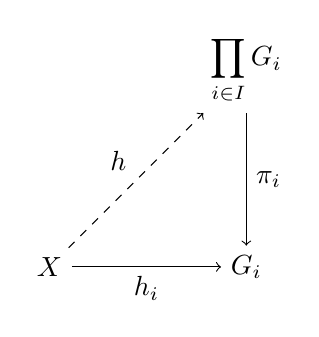
\begin{tikzpicture}[node distance=2.5cm, auto]
	\node (P) {$\displaystyle\prod_{i \in I} \bm{G_i}$};
	\node (Ci) [below of=P] {$\bm{G_i}$};
	\node (X) [left of=Ci] {$\bm{X}$};
	\draw[->] (X) to node [swap] {$h_i$} (Ci);
	\draw[->, dashed] (X) to node {$h$} (P);
	\draw[->] (P) to node {$\pi_i$} (Ci);
\end{tikzpicture}
\end{figure}
\end{prop}
\begin{proof}
Defina a função
	\begin{align*}
	h: X &\to \prod_{i \in I} G_i \\
		x &\mapsto (h_i(x))_{i \in I}.
	\end{align*}
Da propriedade universal para o produto de conjuntos, $h$ é a única função tal que, para todo $i \in I$, $\pi_i \circ h = h_i$. Basta mostrar que $h$ é homomorfismo de grupos. Por simplicidade, apenas a operação $\opb$ em $G$ será explicitada. Sejam $x_1,x_2 \in X$. Então, como $h_i$ são homomorfismos de grupo,
	\begin{equation*}
	h(x_1 \star x_2) = (h_i(x_1 \star x_2))_{i \in I} = (h_i(x_1) \opb_i h_i(x_2))_{i \in I} = h(x_1) \opb h(x_2).
	\end{equation*}
\end{proof}

\subsection{Grupo Livre}

\begin{defi}
Seja $C$ um conjunto. O \emph{conjunto de inversos formais} de $C$ é o conjunto
	\begin{equation*}
	C\inv \coloneqq \set{(c,-1)}{c \in G}.
	\end{equation*}
Os elementos de $C\inv$ são denotados $c\inv \coloneqq (c,-1)$.

Uma \emph{palavra} em $C$ é uma sequência finita $(c_1,\ldots,c_n) \in C^n$. Denota-se $c_1 \cdots c_n$.
\end{defi}

Seja $p=c_1 \cdots c_n$ uma palavra em $C$. A \emph{palavra inversa} de $p$ é a palavra $p\inv \coloneqq c_n\inv \cdots c_1\inv$.

\begin{defi}
Seja $C$ um conjunto e $p_1,p_2 $ palavras em $C \cup C\inv$. A relação de equivalência entre as palavras $p_1$ e $p_2$ é definida por
	\begin{equation*}
	p_1 \sim p_2 \sse p_1p_2\inv \leadsto e.
	\end{equation*}	
\end{defi}

	\begin{equation*}
	C^* \coloneqq \bigcup_{n \in \N} (C \cup C\inv)^n
	\end{equation*}
 Define-se $C^0 = \{e\coloneqq \emptyset\}$.

	\begin{equation*}
	\ger{C} \coloneqq C^*/\sim
	\end{equation*}
	
	A inclusão é definida.
	\begin{align*}
	\func{\iota}{C}{\ger{C}}{c}{[c]}.
	\end{align*}

\begin{prop}[Propriedade Universal]
Seja $C$ um conjunto, $\bm X = (X,\star)$ um grupo e $f: C \to X$ uma função. Então existe um único homomorfismo de grupos $h: \bm{\ger{C}} \to \bm X$ tal que $h \circ \iota = f$ (o diagrama comuta).
\begin{figure}
\centering
\begin{tikzpicture}[node distance=2.5cm, auto]
	\node (C) {$C$};
	\node (G) [above of=C] {$\displaystyle\bm{\ger{C}}$};
	\node (X) [right of=C] {$\bm X$};
	\draw[->] (C) to node [swap] {$f$} (X);
	\draw[->, dashed] (G) to node {$h$} (X);
	\draw[->] (C) to node {$\iota$} (G);
\end{tikzpicture}
\end{figure}
\end{prop}
\begin{proof}
Defina a função
	\begin{align*}
	\func{h}{\ger{C}}{X}{\left[c_1 \cdots c_n\right] }{f(c_1) \star \cdots \star f(c_n)},
	\end{align*}
de modo que $h([e])=e_X$. Então, para todo $c \in C$,
	\begin{equation*}
	h \circ \iota(c) = h (\iota(c)) = h([c])=f(c).
	\end{equation*}
Logo $h \circ \iota = f$. Para mostrar que é um homomorfismo de grupos, sejam $[c_1 \cdots c_n],$ $[d_1 \cdots d_m] \in \ger{C}$. Então
	\begin{align*}
	h([c_1 \cdots c_n][d_1 \cdots d_m]) &= h([c_1 \cdots c_nd_1 \cdots d_m]) \\
		&= f(c_1) \star \cdots \star f(c_n) \star f(d_1) \star \cdots  \star f(d_m) \\
		&= h([c_1 \cdots c_n]) \star h([d_1 \cdots d_m]).
	\end{align*}
Isso mostra a existência. Para mostrar a unicidade, seja $\overline h: \bm{\ger{C}} \to \bm X$ um homomorfismo de grupos tal que $\overline h \circ \iota = f$. Seja $[c_1 \cdots c_n] \in \ger{C}$. Como $[c_1 \cdots c_n] = [c_1] \cdots [c_n] = \iota(c_1) \cdots \iota(c_n)$, segue que
	\begin{align*}
	\overline h ([c_1 \cdots c_n]) &= \overline h(\iota(c_1) \cdots \iota(c_n)) \\
		&= \overline h(\iota(c_1)) \star \cdots \star \overline h(\iota(c_n)) \\
		&= f(c_1) \star \cdots \star f(c_n) \\
		&= h([c_1 \cdots c_n]),
	\end{align*}
o que implica que $\overline h = h$.
\end{proof}

\subsection{Coproduto de Grupos}

\begin{defi}
Seja $(\bm{G_i})_{i \in I}$ uma família de grupos. O \emph{coproduto} da família $(\bm{G_i})_{i \in I}$ é o par
	\begin{equation*}
	\coprod_{i \in I} \bm{G_i} \coloneqq \left(G,\opb \right),
	\end{equation*}
em que $G \coloneqq \ger{\coprod_{i \in I} G_i}$ é o grupo livre sobre o coproduto de conjuntos $\coprod_{i \in I} G_i$ e
	\begin{align*}
	\func{\opb}{G \times G}{G}{([p_1],[p_2])}{[p_1p_2]}.
	\end{align*}
\end{defi}

\begin{prop}[Propriedade Universal]
Sejam $(\bm{G_i})_{i \in I}$ uma família de grupos, $\bm X = (X,\star)$ um grupo e, para todo $i \in I$, $h_i: \bm{G_i} \to \bm X$ um homomorfismo de grupos. Então existe um único homomorfismo de grupos $h: \coprod_{i \in I} \bm{G_i} \to \bm X$ tal que, para todo $i \in I$, $h \circ \iota_i = h_i$ (o diagrama comuta).
\begin{figure}
\centering
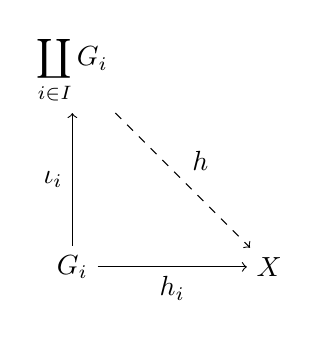
\begin{tikzpicture}[node distance=2.5cm, auto]
	\node (Ci) {$\bm{G_i}$};
	\node (S) [above of=Ci] {$\displaystyle\coprod_{i \in I} \bm{G_i}$};
	\node (X) [right of=Ci] {$\bm X$};
	\draw[->] (Ci) to node [swap] {$h_i$} (X);
	\draw[->, dashed] (S) to node {$h$} (X);
	\draw[->] (Ci) to node {$\iota_i$} (S);
\end{tikzpicture}
\end{figure}
\end{prop}
\begin{proof}
Defina a função
	\begin{align*}
	\func{h}{\ger{\coprod_{i \in I} G_i}}{X}{\left[(g_1,i_1) \cdots (g_n,i_n)\right]}{h_{i_1}(g_1) \star \cdots \star h_{i_n}(g_n)}.
	\end{align*}

Por simplicidade, seja $G \coloneqq \ger{\coprod_{i \in I} G_i}$. Para mostrar que $h$ é homomorfismo, sejam $[(g_1,i_1) \cdots (g_n,i_n)]$ e $[(g'_1,i'_1) \cdots (g'_m,i'_m)] \in G$. Então
	\begin{align*}
	&h([(g_1,i_1) \cdots (g_n,i_n)][(g'_1,i'_1) \cdots (g'_m,i'_m)]) \\
		&= h([(g_1,i_1) \cdots (g_n,i_n)(g'_1,i'_1) \cdots (g'_m,i'_m)]) \\
		&= h_{i_1}(g_1) \star \cdots \star h_{i_n}(g_n) \star h_{i'_1}(g'_1) \star \cdots \star h_{i'_n}(g'_n) \\
		&= h([(g_1,i_1) \cdots (g_n,i_n)]) \star h([(g'_1,i'_1) \cdots (g'_m,i'_m)]).
	\end{align*}
\end{proof}








































\cleardoublepage
\section{Construções Específicas}

\subsection{Grupo Simples e Subgrupo Normal Maximal}

\begin{defi}
Um \emph{grupo simples} é um grupo não-trivial $\bm G$ cujos únicos subgrupos normais são $\bm{\{e\}}$ e $\bm G$.
\end{defi}

\begin{defi}
Seja $\bm G$ um grupo. Um subgrupo normal \emph{maximal} de $\bm G$ é um subgrupo normal próprio $\bm M \idepro \bm G$ que satisfaz
	\begin{enumerate}
	\item (Maximalidade) Para todo $\bm N \ide \bm G$,
		\begin{equation*}
		M \subseteq N \Rightarrow N = M \ou N = G.
		\end{equation*}
	\end{enumerate}
\end{defi}

\begin{prop}
Sejam $\bm G$ um grupo e $\bm M \ide \bm G$ um subgrupo normal. Então $\bm M$ é maximal se, e somente se, $\bm{G/M}$ é simples.
\end{prop}
\begin{proof} Consideremos a projeção canônica
	\begin{align*}
	\pi: G &\to G/M \\
		 g &\mapsto gM.
	\end{align*}
($\Rightarrow$) Suponhamos que $\bm M$ é maximal. Então $\bm M$ é um subgrupo próprio, o implica que $\bm{G/M}$ é não-trivial. Seja $\bm N \ide \bm{G/M}$. Sabemos que $\bm{\pi^{-1}(N)} \ide \bm G$ (\ref{alge:prop.gru.hominv}). Como $[e] \in N$, então $\pi^{-1}(e) \subseteq \pi^{-1}(N)$. Notando que $\pi^{-1}([e])=\nuc(\pi) = M$, segue que $M \subseteq \pi^{-1}(N)$. Como $\bm M$ é maximal, segue que $\pi^{-1}(N) = N$ ou $\pi^{-1}(N) = G$. Notemos que $N=\pi(\pi^{-1}(N))$, pois $\pi$ é sobrejetiva. No primeiro caso, $N = \pi(\pi^{-1}(N)) = \pi(M) = \{[e]\}$. No segundo caso, $N = \pi(\pi^{-1}(N)) = \pi(G) = G/M$. Portanto $\bm{G/M}$ é simples.

\noindent
($\Leftarrow$) Suponhamos que $\bm{G/M}$ é simples. Seja $\bm N \ide \bm G$ tal que $M \subseteq N$. Como $\pi$ é homomorfismo de grupos sobrejetivo, ssegue que $\pi(N) \ide \bm{G/M}$ (\ref{alge:prop.gru.hom}). Como $\bm{G/M}$ é simples, então $\pi(N) = \{[e]\}$ ou $\pi(N) = G/M$. No primeiro caso, $N = \nuc(\pi) = M$. No segundo caso, $N = \pi^{-1}(\pi(N)) = \pi^{-1}(N) = G$. Logo $\bm M$ é maximal.
\end{proof}

\begin{conj}
Sejam $\bm G$ um grupo e $\bm N \idepro \bm G$ um subgrupo normal próprio. Então $\bm G$ tem subgrupo normal maximal.
\end{conj}
\begin{proof}
Usaremos o lema de Zorn. Seja $P \subseteq \p(G)$ o conjunto de todos os subconjuntos $S \subset G$ tais que $\bm S \idepro \bm G$. Então $(P,\subseteq)$ é um conjunto parcialmente ordenado com a contenção de conjuntos usual. Agora, seja $(C)_{i \in I}$ uma cadeia de $(P,\subseteq)$. Consideremos o conjunto $C \coloneqq \bigcup_{i \in I} C_i$. Como 

Notemos que $P$ não é vazio, pois $N \in P$. Seja 



Então $P$ tem elemento maximal.
\end{proof}






\subsection{Sequência subnormal}

\begin{defi}
Seja $\bm G$ um grupo. Uma \emph{sequência subnormal} de $\bm G$ é uma sequência finita $(\bm{N_i})_{i \in \inte_n}$ de subgrupos de $\bm G$ que satisfaz
	\begin{equation*}
	\bm{\{e\}} = \bm{N_0} \ide \cdots \ide \bm{N_n} = \bm G.
	\end{equation*}
O grupo $\bm{N_{i+1}/N_i}$ é o $i$-ésimo \emph{grupo fator} da sequência.
Uma \emph{sequência normal} é uma sequência subnormal em que, para todo $i \in \inte_n$, $\bm{N_i} \ide \bm G$.

Uma sequência subnormal \emph{estrita} de $\bm G$ é uma sequência subnormal $(\bm{N_i})_{i \in \inte_n}$ de $\bm G$ que satisfaz
	\begin{equation*}
	\bm{\{e\}} = \bm{N_0} \idepro \cdots \idepro \bm{N_n} = \bm G.
	\end{equation*}
	
O comprimento
\end{defi}



\subsection{Conjunto gerador}

\begin{defi}
Seja $\bm G$ um grupo e $S \subseteq G$ um conjunto. O grupo \emph{gerado} por $S$ é o grupo $\bm{\langle S \rangle} \leq \bm G$ em que
	\begin{equation*}
	\langle S \rangle \coloneqq \{s_1 \cdots s_n : n \in \N,\ s_i \in S \ou s_i\inv \in S\}.
	\end{equation*}
	\begin{equation*}
	\langle S \rangle \coloneqq \left\{\bigopb_{i \in \inte_n} s_i : n \in \N,\ s_i \in S \ou s_i\inv \in S\right\}.
	\end{equation*}
\noindent
Um \emph{conjunto gerador} de $\bm G$ é um conjunto $S \subseteq G$ tal que $\langle S \rangle = G$.
\end{defi}










\subsection{Grupos Simétricos e Alternados}

\begin{defi}
Seja $C$ um conjunto. O \emph{grupo simétrico} de $C$ é o par $\bm{\simm{C}} = (\simm{C},\circ)$, em que	
	\begin{equation*}
	\simm{C} \coloneqq \set{p: C \to C}{\exists p\inv: C \to C}
	\end{equation*}
é o conjunto de todas as bijeções entre $C$ e $C$, e $\circ$ é a composição de funções. Seja $\alpha$ um número cardinal. Para $C = \alpha$, usa-se a notação $\sime_{\alpha} \coloneqq \simm{\alpha}$.
\end{defi}

\begin{prop}
	Seja $C$ um conjunto. O grupo simétrico $\bm{\simm{C}}$ é um grupo.
\end{prop}
\begin{proof}
	Se $C=\emptyset$, então $\simm{C}=\{\emptyset\}$. Assim, como $\emptyset \circ \emptyset = \emptyset$, segue que $\circ$ é operação binária em $\{\emptyset\}$. Ainda, segue que $\circ$ é associativa, pois $(\emptyset \circ \emptyset) \circ \emptyset = \emptyset \circ (\emptyset \circ \emptyset)$; tem elemeno neutro $\emptyset$, pois $\emptyset \circ \emptyset = \emptyset$, e que todo elemento tem inverso, pois $\emptyset\inv = \emptyset$.

	Suponhamos, então, que $C \neq \emptyset$ e sejam $p_1,p_2 \in \simm{C}$. Como $p_1$ e $p_2$ são bijeções, a função $p_2 \circ p_1: C \to C$ é uma bijeção entre $C$ e $C$ (\ref{prop:comp.func.inj} e \ref{prop:comp.func.sobr}) e, portanto, $p_2 \circ p_1 \in \simm{C}$. Isso mostra que $\circ$ é uma operação binária em $\simm{C}$. A composição de funções é associativa, pois, para todos $p_1,p_2,p_3 \in \simm{C}$, $p_3 \circ (p_2 \circ p_1) = (p_3 \circ p_2) \circ p_1$ (\ref{prop:comp.func.asso}). Ainda, notemos que $\id_C$ é o elemento neutro de $\bm{\simm{C}}$, pois, para todo $p \in \simm{C}$, vale $p \circ \id_C = \id_C \circ p = p$ (\ref{prop:id.comp.func}). Por fim, como $p$ é uma bijeção, existe função inversa $p\inv: C \to C$ que é bijeção entre $C$ e $C$ (\ref{prop:func.inv.esq} e \ref{prop:func.inv.dir}); logo existe $p\inv \in \simm{C}$ tal que $p \circ p\inv = p\inv \circ p = \id_C$. Portanto concluímos que $\bm{\simm{C}}$ é um grupo.
\end{proof}

\begin{prop}
	Sejam $A$ e $B$ conjuntos tais que $\card{A} = \card{B}$. Então
	\begin{equation*}
	\bm{\simm{A}} \simeq \bm{\simm{B}}.
	\end{equation*}
\end{prop}
\begin{proof}
	Seja $\phi: A \to B$ uma bijeção e considere a função
	\begin{align*}
	h : \simm{A} &\to \simm{B} \\
			p &\mapsto \phi \circ p \circ \phi\inv.
	\end{align*}
Primeiro notemos que $h$ é homomorfismo de grupos. Sejam $p_1,p_2 \in \simm{A}$. Então
	\begin{align*}
	h(p_2 \circ p_1)(c) &= \phi \circ (p_2 \circ p_1) \circ \phi^{-1} \\
			&= \phi \circ (p_2 \circ \phi\inv \circ \phi \circ p_1) \circ \phi^{-1} \\
			&= (\phi \circ p_2 \circ \phi\inv) \circ (\phi \circ p_1 \circ \phi\inv) \\
			&= h(p_2) \circ h(p_1).
	\end{align*}
Portanto $h$ é um homomorfismo de grupos entre $\bm{\simm{A}}$ e $\bm{\simm{B}}$.

Agora notemos que $h$ é uma bijeção. A inversa de $h$ é a função
	\begin{align*}
	h\inv : \simm{B} &\to \simm{A} \\
			p &\mapsto \phi\inv \circ p \circ \phi,
	\end{align*}
pois, para todo $p \in \simm{B}$,
	\begin{align*}
	(h \circ h\inv) (p) &= h (h\inv(p)) \\
			&= \phi \circ h\inv(p) \circ \phi\inv \\
			&= \phi \circ (\phi\inv \circ p \circ \phi) \circ \phi\inv \\
			&= p \\
			&= \id_{\simm{B}}(p),
	\end{align*}
o que mostra que $h \circ h\inv = \id_{\simm{B}}$, e, para todo $p \in \simm{A}$,
	\begin{align*}
	(h\inv \circ h) (p) &= h\inv (h(p)) \\
			&= \phi\inv \circ h(p) \circ \phi \\
			&= \phi\inv \circ (\phi \circ p \circ \phi\inv) \circ \phi \\
			&= p \\
			&= \id_{\simm{A}}(p),
	\end{align*}
o que mostra que $h\inv \circ h = \id_{\simm{A}}$. Assim, está provado que $h$ é isomorfismo entre $\bm{\simm{A}}$ e $\bm{\simm{B}}$.
\end{proof}

	Essa proposição mostra que podemos estudar somente os grupos simétricos dos números cardinais, pois isso será equivalente a estudar qualquer grupo simétrico. Em particular, para todo conjunto finito, podemos estudar seu grupo simétrico considerando somente o grupo simétrico $\bm\sime_n$, em que $n$ é o número de elementos do conjunto. A partir de agora, as proposições serão considerando esses grupos $\bm\sime_n$.

\begin{prop}
	Seja $n \in \N$. Então $|\sime_n|=n!$.
\end{prop}

\begin{teo}
	Seja $\bm G$ um grupo. Então
	\begin{equation*}
	\bm G \lesssim \bm{\simm{G}}.
	\end{equation*}
\end{teo}
\begin{proof}
	Consideremos a função
	\begin{align*}
	h: G \to \simm{G} & \\
		g \mapsto h(g): & G \to G \\
									&\ x \mapsto g \opb x \\
	\end{align*}
Primeiro, devemos mostrar que $h(g) \in \simm{G}$, para que $h$ esteja bem definida. Para isso, notemos que $h(g)$ está bem definida, já que, para todo $x \in G$, $g \opb x \in G$. Ainda, $h(g)$ é uma bijeção, pois $h(g)\inv = h(g\inv)$, já que, para todo $x \in G$,
	\begin{equation*}
	(h(g) \circ h(g)\inv)(x) = h(g)((h(g)\inv)(x)) = h(g)(g\inv \opb x) = g \opb g\inv \opb x = x = \id_G,
	\end{equation*}
o que mostra que $h(g) \circ h(g)\inv = \id_G$, e
	\begin{equation*}
	(h(g)\inv \circ h(g))(x) = h(g)\inv((h(g)(x)) = h(g)\inv(g \opb x) = g\inv \opb g \opb x = x = \id_G,
	\end{equation*}
o que mostra que $h(g)\inv \circ h(g) = \id_G$. Isso mostra que $h(g)$ é uma bijeção e, portanto, $h(g) \in \simm{G}$.

	Agora, notemos que $h$ é um homomorfismo de grupos, pois, para todos $g_1,g_2 \in G$, segue que, para todo $x \in G$,
	\begin{align*}
	h(g_1 \opb g_2)(x) &= (g_1 \opb g_2) \opb x \\
	&= g_1 \opb (g_2 \opb x) \\
	&= h(g_1)(g_2 \opb x) \\
	&= h(g_1)(h(g_2)(x)) \\
	&= (h(g_1) \circ h(g_2))(x),
	\end{align*}
o que mostra que $h(g_1 \opb g_2) = h(g_1) \circ h(g_2)$. Por fim, notemos que $h$ é injetiva, já que, se $g \in G$ é tal que $h(g)=id_G$, então, para todo $x \in G$,
	\begin{equation*}
	g \opb x = h(g)(x) = \id_G(x) = x,
	\end{equation*}
o que mostra que $g=e_G$ e, portanto, que $\nuc(h)=\{e_G\}$.
\end{proof}

	Esse teorema é um teorema muito importante, pois ele mostra que, de certa forma, todo grupo é um subconjunto de permutações. Por causa disso que grupos são pensados como os objetos algébricos que modelam a simetria.

\subsubsection{Permutações e Órbitas}

\begin{defi} Seja $n \in \N$. Uma \emph{permutação} de $n$ objetos é um elemento $p \in \sime_n$, denotado por
	\begin{equation*}
	p = \begin{pmatrix}
				1 & 2 & \cdots & n-1 & n \\
				p(1) & p(2) & \cdots &  p(n-1)  & p(n)
			\end{pmatrix}.
	\end{equation*}
\end{defi}

\begin{nota}
	Seja $n \in \N$. A composição de duas permutações $p_1,p_2 \in \sime_n$, quando representadas na notação acima, é denotada
	\begin{equation*}
	p_2 \circ p_1 = \bigl(\begin{smallmatrix}
				1 & 2 & \cdots & n-1 & n \\
				p_2(1) & p_2(2) & \cdots &  p_2(n-1)  & p_2(n)
			\end{smallmatrix}\bigr)
			\bigl(\begin{smallmatrix}
				1 & 2 & \cdots & n-1 & n \\
				p_1(1) & p_1(2) & \cdots &  p_1(n-1)  & p_1(n)
			\end{smallmatrix}\bigr).
	\end{equation*}
\end{nota}

\begin{defi}
	Sejam $n \in \N$ e $p \in \sime_n$. A \emph{matriz de permutação} de $p$ é a matriz $[p] \in \mathbb M_n (\Z)$ cujas entradas são dadas por
	\begin{equation*}
		[p]_{i,j} = \delta_{i,p(j)} = \begin{cases}
												1 & i=p(j) \\
												0 & i \neq p(j).
												\end{cases}
	\end{equation*}
	O \emph{conjunto das matrizes de permutação} de $\sime_n$ é o conjunto
	\begin{equation*}
		[\sime_n] \coloneqq \{[p] : p \in \sime_n\}.
	\end{equation*}
\end{defi}

\begin{prop}
	Seja $n \in \N$. Então o par $\bm{[\sime_n]}=([\sime_n],\cdot)$, em que $\cdot$ é o produto de matrizes, é um grupo, e
	\begin{equation*}
	\bm{\sime_n} \simeq \bm{[\sime_n]}.
	\end{equation*}
\end{prop}
\begin{proof}
	Primeiro, notemos que, para todos $p,q \in \sime_n$,
	\begin{equation*}
	[p][q]_{i,j} = \bigplus_{k=1}^n [p]_{i,k}[q]_{k,j} = \bigplus_{k=1}^n \delta_{i,p(k)}\delta_{k,p(j)}.
	\end{equation*}
	Mas o produto $\delta_{i,p(k)}\delta_{k,p(j)}$ é igual a 1 se, e somente se, $i=p(k)$ e $k=q(j)$. Como $p$ é bijeção, a segunda consição é equivalente a $p(k)=pq(j)$, e isso mostra que as duas consições são equivalentes a $i=p(k)=pq(j)$. Como $p$ é bijeção, para cada $i \in \inte_n$, $k=p\inv(i)$ é o único $k \in \inte_n$ tal que a condição é satisfeita, e segue que
	\begin{equation*}
	[p][q]_{i,j} = \bigplus_{k=1}^n \delta_{i,p(k)}\delta_{k,p(j)} = \bigplus_{k=1}^n \delta_{i,pq(j)} = [pq]_{i,j}.
	\end{equation*}
e, como $pq \in \sime_n$, então $[p][q]=[pq] \in [\sime_n]$. Isso mostra que o produto de matrizes é uma operação binária em $[\sime_n]$. Agora, disso segue que $[p][p\inv]=[pp\inv]=[id]$

MOATRAR QUE O INVERSO DE P ESTA NO GRUPO




Disso, segue que $\bm{[\sime_n]}$ é um grupo, pois é subgrupo de $\mathbb M_n(\Z)$. Por fim, consideremos a função
	\begin{align*}
	h: \sime_n &\to [\sime_n] \\
			p &\mapsto [p].
	\end{align*}
Note que que $h$ é homomorfismo, pois, para todos $p,q \in \sime_n$,
	\begin{equation*}
	h(pq) = [pq]= [p][q] = h(p)h(q).
	\end{equation*}
Ainda, $h$
\end{proof}

\begin{defi}
	Sejam $n \in \N$, $p \in \sime_n$ e $m \in \inte_n$. A \emph{órbita de $m$ sob $p$} é o conjunto
	\begin{equation*}
	\orb_p(m) \coloneqq \{p^k(m) : k \in \Z\}.
	\end{equation*}
O \emph{período} da órbita $\orb_p(m)$ é o número $\card{\orb_p(m)}$. Uma \emph{órbita trivial} é uma órbita de período $1$. Uma órbita de $p$ é a órbita de um elemento $m \in \inte_n$ sob $p$.

	O \emph{conjunto de órbitas} de $p$ é o conjunto
	\begin{equation*}
	\orb_p \coloneqq \{\orb_p(m) : m \in \inte_n\}.
	\end{equation*}
\end{defi}

\begin{prop}
	Sejam $n \in \N$ e $p \in \sime_n$. O conjunto $\orb_p$ é uma partição de $\inte_n$.
\end{prop}
\begin{proof}
	Primeiro, notemos que $m \in \orb_p(m)$ e, portanto, $\emptyset \nsubseteq \orb_p$. Ainda, $\bigcup_{m \in \inte_n} \orb_p(m) = \inte_n$, já que, para todo $m \in inte_n$, $m \in \orb_p(m)$, o que mostra que $\inte_n \subseteq \bigcup_{m \in \inte_n}$ e, para todo $l \in \bigcup_{m \in \inte_n} \orb_p(m)$, existe $m \in \inte_n$ tal que $l \in \orb_p(m)$ e, portanto, existe $k \in \N$ tal que $l=p^k(m) \in \inte_n$, o que mostra que $\bigcup_{m \in \inte_n} \subseteq \inte_n$. Por fim, sejam $o_1,o_2 \in \orb_p$. Então existem $m_1,m_2 \in \inte_n$ tais que $o_1=\orb_p(m_1)$ e $o_2=\orb_p(m_2)$. Se existe $l \in \orb_p(m_1) \cap \orb_p(m_2)$, então existem $k_1,k_2 \in \Z$ tais que $l=p^{k_1}(m_1)=p^{k_2}(m_2)$. Assim, segue que $m_1=p^{k_2-k_1}(m_2)$ e, portanto, $m_1 \in \orb_p(m_2)$. Mas isso implica que $\orb_p(m_1) \subseteq \orb_p(m_2)$; a inclusão contrária é análoga e concluímos que $\orb_p(m_1) = \orb_p(m_2)$. Logo $\orb_p$ é uma partição de $\inte_n$.
\end{proof}

\subsubsection{Permutações, Ciclos e Transposições}

\begin{defi}
	Sejam $n,k \in \N$. Um \emph{ciclo} de $\sime_n$ é um elemento $c \in \sime_n$ para o qual existe $m \in \inte_n$ tal que, para todo $m' \in \inte_n$, $c(m')=m'$ ou existe $d \in \inte_n$ tal que $m'=c^d(m)$. O \emph{comprimento} de um ciclo é a ordem desse ciclo. Um ciclo $c$ cujo comprimento é $k$ é denotado
	\begin{equation*}
	c = \bigl(m \ c(m) \ c^2(m) \ \cdots \  c^{k-2}(m) \ c^{k-1}(m)\bigr).
	\end{equation*}
\end{defi}


\begin{prop}
	Sejam $n \in \N$.
	\begin{enumerate}
	\item Se $c_1,c_2 \in \sime_n$ são ciclos disjuntos, então $c_2 \circ c_1 = c_1 \circ c_2$.
	\end{enumerate}
\end{prop}

\begin{prop}[Fatoração de Permutação]
	Seja $n \in \N$ e $p \in \sime_n$. Então existem únicos ciclos $c_1,\ldots,c_k \in \sime_n$ disjuntos dois a dois tais que $p=c_1 \circ \cdots \circ c_k$.
\end{prop}
\begin{proof}
	Seja $k \coloneqq \card{\orb_p}$. O cojunto $\orb_p$ particiona $\inte_n$. Sejam $(o_k)_{i \in \inte_k}$ uma indexação de $\orb_p$ e $m_1,\cdot,m_k \in \inte_n$ tais que $o_i=\orb_p(m_i)$ para todo $i \in \inte_k$, e seja $k_i \coloneqq \card{\orb_p(m_i)}$. Definamos $c_i \coloneqq  \bigl( m_i \ \cdots \  p^{k_i-1}(m_i)\bigr)$. Então segue que
	\begin{equation*}
	p = \bigtimes_{i=1}^k \bigl( m_i \ \cdots \  p^{k_i-1}(m_i)\bigr) = \bigtimes_{i=1}^k c_i.
	\end{equation*}
\end{proof}



\subsection{Grupos Cíclicos}

\subsection{Grupos Diedrais}


\cleardoublepage
\subsection{Ações de Grupos}

A noção de uma ação de grupo, de certa forma, generaliza uma estratégia usada na demonstração do teorema de que todo grupo é isomorfo a um subgrupo de seu grupo simétrico.

\begin{defi}
Sejam $X$ um conjunto e $\bm G$ um grupo. Uma \emph{ação (à esquerda)} de $\bm G$ em $X$ é uma função
	\begin{align*}
	\func{\age}{G \times X}{X}{(g,x)}{g\age x}
	\end{align*}
que satisfaz
\begin{enumerate}
\item (Identidade) Para todo $x \in X$,
	\begin{equation*}
	e \age x = x;
	\end{equation*}
\item (Compatibilidade) Para todos $g_0,g_1 \in G$ e $x \in X$,
	\begin{equation*}
	(g_1g_0) \age x = g_1 \age (g_0 \age x).
	\end{equation*}
\end{enumerate}
Um grupo $\bm G$ \emph{age} em o conjunto $X$ se, e somente se, existe uma ação de $\bm G$ em $X$.
\end{defi}

Analogamente, uma ação à direita pode ser definida, mas toda ação à direita pode ser traduzida em uma ação à esquerda, de modo que é suficiente estudar somente ações à esquerda.

\begin{prop}
Sejam $X$ um conjunto, $\bm G$ um grupo, $A$ uma ação de $\bm G$ em $X$ e $g \in G$. Então a função
	\begin{align*}
	\func{g\age}{X}{X}{x}{g\age x}
	\end{align*}
é uma bijeção. Equivalentemente, $g\age \in \simm{X}$.
\end{prop}

\begin{prop}
Sejam $X$ um conjunto, $\bm G$ um grupo e $\age$ uma ação de $\bm G$ em $X$. Então a função
%	\begin{align*}
%	\func{\phi}{G}{\simm{X}}{g}{g\age}
%	\end{align*}
	\begin{align*}
	h: G &\to \simm{X} \\
			g &\mapsto g\age: X \to X\\
				&\qquad\qquad\; x \mapsto g\age x.
	\end{align*}
é um homomorfismo de grupos de $\bm G$ para $\bm{\simm{X}}$.
\end{prop}
\begin{proof}
Sejam $g_1,g_0 \in G$ e $x \in X$. Então
	\begin{equation*}
	h(g_1g_0)(x) =(g_1g_0) \age x = g_1 \age (g_0 \age x) = h(g_1)(h(g_0)(x)) = h(g_1) \circ h(g_0)(x),
	\end{equation*}
logo $h(g_1g_0)=h(g_1) \circ h(g_0)$.
\end{proof}

Sob a ótica desse teorema, as propriedades de uma ação de grupos podem ser escritas
	\begin{enumerate}
	\item $e\age = \id$;
	\item Para todos $g_0,g_1 \in G$,
		\begin{equation*}
		(g_1g_0)\age = g_1\age \circ g_0\age.
		\end{equation*}
	\end{enumerate}

\begin{defi}
Sejam $X$ um conjunto, $\bm G$ um grupo que age em $X$ e $x \in X$. A \emph{órbita} de $x$ sob $\bm G$ é o conjunto
	\begin{equation*}
	G \age x \coloneqq \set{g\age x}{g \in G}.
	\end{equation*}
\end{defi}



\begin{equation*}
G_x = \set{g \in G}{g\age x = x} = h\inv(\{\id\}) = \nuc(h).
\end{equation*}















\newpage

\chapter{Anéis}

\section{Anel}

\begin{defi}
	Um \emph{anel} é uma tripla $\bm A=(A,+,\cdot)$ em que
	\begin{enumerate}
	\item $(A,+)$ é um grupo comutativo com elemento neutro chamado de \emph{zero} ou \emph{nulidade} e representado por $0$ (ou $0_A$, caso exista ambiguidade).
	\item $(A,\cdot)$ é um monoide comutativo com elemento neutro chamado de \emph{um} ou \emph{unidade} e representado por $1$ (ou $1_A$, caso exista ambiguidade).
	\item A operação $\cdot$ é distributiva sobre $+$.
	\end{enumerate}
As operações $+$ e $\cdot$ são chamadas, respectivamente, de \emph{adição} e \emph{multiplicação}. A imagem de dois elementos $a_1,a_2 \in A$ pela adição é chamada de \emph{soma} de $a_1$ e $a_2$ e denotada por $a_1+a_2$. A imagem de $a_1,a_2$ pela multiplicação é chamada de \emph{produto} de $a_1$ e $a_2$ e denotada por $a_1 \cdot a_1$ ou $a_1a_2$.
\end{defi}

	Um comentário sobre os elementos neutros $0$ e $1$. Se $0=1$, o anel será trivial, mas garantimos esse anel na definição pois, mais para frente, quando virmos anéis quocientes, vai ser proveitoso que qualquer anel quociente seja um anel, e se quocientarmos um anel por ele mesmo, temos o anel trivial.

\begin{nota}
	Como $(A,+)$ é um grupo, denotaremos o inverso de um elemento $a \in A$ sob $+$ por $-a$, e escreveremos $a_1 - a_2$ para $a_1 + (-a_2)$. Ainda, a multiplicação tem preferência na notação; ou seja, $a_1a_2+a_3 = (a_1 \cdot a_2)+a_3$ e $-a_1a_2 = -(a_1 \cdot a_2)$. Denotaremos o inverso de um elemento $a \in A$ sob $\cdot$ por $a^{-1}$, se ele existir, pois sabemos que é único (\ref{prop:unic.inv}). Os símbolos operatórios relativos à adição e à multiplicação serão, respectivamente, $\bigplus$ e $\bigtimes$. Caso não haja ambiguidade, denotaremos um anel pelo símbolo que denota seu conjunto escrito em negrito, como em $\bm A=(A,+,\cdot)$.
\end{nota}

\begin{prop}
	Seja $\bm A$ um anel. Então, para todo $a,b \in A$,
	\begin{enumerate}
	\item $0 \cdot a = 0$;
	\item $-(a \cdot b) = (-a) \cdot b$.
	\end{enumerate}
\end{prop}
\begin{proof}
	\begin{enumerate}
	\item
		\begin{align*}
		0 \cdot a &= 0 \cdot a + 0 \\
			&= 0 \cdot a + (0 \cdot a - 0 \cdot a) \\
			&= (0 \cdot a + 0 \cdot a) - 0 \cdot a \\
			&= (0+0) \cdot a - 0 \cdot a \\
			&= 0 \cdot a - 0 \cdot a \\
			&= 0.
		\end{align*}
	\item
		\begin{align*}
		-(a \cdot b) &= -(a \cdot b) + 0 \\
			&= -(a \cdot b) + 0 \cdot b \\
			&= -(a \cdot b) + (a - a) \cdot b \\
			&= -(a \cdot b) + (a \cdot b + (-a) \cdot b) \\
			&= (-(a \cdot b) + a \cdot b) + (-a) \cdot b \\
			&= 0 + (-a) \cdot b \\
			&= (-a) \cdot b.
		\end{align*}
	\end{enumerate}
\end{proof}

\begin{defi}
	Seja $\bm A$ um anel. O conjunto dos elementos invertíveis sob multiplicação de $\bm A$ é denotado por $A^*$.
\end{defi}

\begin{prop}
	Seja $\bm A$ um anel. O par $(A^*,\cdot|_{A^* \times A^*})$ é um grupo comutativo.
\end{prop}
\begin{proof}
	O par $(A,\cdot)$ é um monoide comutativo com elemento neutro $1$. Portanto segue que o par $(A^*,\cdot|_{A^* \times A^*})$ é um grupo. Como $(A,\cdot)$ é comutativo, então $(A^*,\cdot|_{A^* \times A^*})$ também o é.
\end{proof}

\begin{defi}
	Um \emph{domínio de integridade} (ou \emph{domínio}) é um anel $\bm A$ em que
	\begin{equation*}
	\forall a_1, a_2 \in A \qquad a_1 \cdot a_2 = 0 \Rightarrow a_1=0 \text{\ \ ou\ \ } a_2=0.
	\end{equation*}
\end{defi}

\begin{defi}
	Um \emph{corpo} é um anel $\bm A$ em que $(A \setminus \{0\},\cdot)$ é um grupo.
\end{defi}

\begin{prop}
\label{prop:corp.dom}
	Seja $\bm A$ um corpo. Então $\bm A$ é um domínio.
\end{prop}
\begin{proof}
	Sejam $a_1,a_2 \in A$ tais que $a_1 \cdot a_2=0$. Suponhamos que $a_2 \neq 0$. Então existe $a_2^{-1} \in A$ e temos
	\begin{equation*}
	\begin{split}
	a_1 &= a_1 \cdot 1 \\
		&= a_1 \cdot (a_2 \cdot a_2^{-1}) \\
		&= (a_1 \cdot a_2) \cdot a_2^{-1}\\
		&= 0 \cdot a_2^{-1} \\
		&= 0.
	\end{split}
	\end{equation*}
	Logo, se $a_1 \cdot a_2=0$, $a_1=0$ ou $a_2=0$.
\end{proof}

\begin{prop}[Lei do corte em domínios]
	Seja $\bm A$ um domínio e $a,a_1,a_2 \in A$, $a \neq 0$. Então
	\begin{equation*}
	aa_1 = aa_2 \Rightarrow a_1=a_2
	\end{equation*}
\end{prop}
\begin{proof}
	Se $aa_1 = aa_2$, então $-aa_1 = -aa_2$. Portanto
	\begin{equation*}
	a(a_1-a_2) = aa_1 -aa_2 = aa_1 -aa_1 = 0.
	\end{equation*}
Logo, como $\textbf{A}$ é um domínio e $a \neq 0$, temos que $a_1-a_2=0$, o que implica $a_1=a_2$.
\end{proof}

	Essa proposição é interessante pois, mesmo sem exigir que $(A \setminus \{0\},\cdot)$ seja um grupo, como no caso de $\textbf{A}$ ser um corpo, se $\textbf{A}$ for um domínio, vale a lei do corte da multiplicação para elementos de $A \setminus \{0\}$.

\section{Subanel}

\begin{defi}
Seja $\bm A=(A,+,\times)$ um anel. Um \emph{subanel} de $\bm A$ é um anel $\bm S=(S,+_S,\times_S)$ em que $S \subseteq A$, $+_S = +|_{S \times S}$ e $\times_S = \times|_{S \times S}$. Denota-se $\bm S \leq \bm A$. Um subanel \emph{próprio} de $\bm A$ é um subanel $\bm S \leq \bm A$ em que $S$ é um conjunto próprio de $A$ ($S \subset A$). Denota-se $\bm S < \bm A$.
\end{defi}

\begin{prop}
Sejam $\bm A=(A,+,\times)$ um anel e $S \subseteq A$. Então
	\begin{equation*}
	\bm S=(S,+|_{S \times S},\times|_{S \times S})
	\end{equation*}
é um anel com $1 \in S$ se, e somente se,
	\begin{enumerate}
	\item $(S,+|_{S \times S})$ é um subgrupo comutativo de $(A,+)$:
			\begin{enumerate}
			\item (Não-vacuidade) $S \neq \emptyset$;
			\item (Fechamento) $\forall s_1,s_2 \in S \qquad s_1 + s_2 \in S$;
			\item (Invertibilidade) $\forall s \in S \qquad -s \in S$;
			\end{enumerate}
	\item $(S,\times|_{S \times S})$ é um submonoide comutativo de $(A,\times)$ com $1 \in S$:
			\begin{enumerate}
			\item (Identidade) $1 \in S$;
			\item (Fechamento) $\forall s_1,s_2 \in S \qquad s_1 \times s_2 \in S$.
			\end{enumerate}
	\end{enumerate}
\end{prop}
\begin{proof}
($\Rightarrow$) Suponhamos que $\bm S$ é um anel com $1 \in S$.
(Subgrupo) Como $S \subseteq A$ e $(S,+|_{S \times S})$ um grupo comutativo, então é um subgrupo de $(A,+)$ por definição de subgrupo (o que é equivalente às propriedades listadas) e é comutativo (\ref{alge:prop.subgru})).
(Subanel)  Como $S \subseteq A$ e $(S,\times|_{S \times S})$ um monoide comutativo com $1 \in S$, então é um submonoide de $(A,\times)$ por definição de submonoide (o que é equivalente às propriedades listadas) e é comutativo (\ref{alge:prop.submon}).

($\Leftarrow$) Suponhamos, agora, que $(S,+|_{S \times S})$ é subgrupo comutativo de $(A,+)$ e $(S,\times_{S \times S})$ é submonoide comutativo de $(A,\times)$.
(Grupo comutativo) Como $(S,+|_{S \times S})$ é subgrupo comutativo, então é um grupo comutativo por definição de subgrupo. (Monoide comutativo) Como $(S,\times|_{S \times S})$ é submonoide comutativo, então é um monoide comutativo por definição de monoide. (Distributividade) Sejam $s_1,s_2,s_3 \in S$. Então
	\begin{align*}
	s_1 \times|_{S \times S} (s_2 +|_{S \times S} s_3) &= s_1 \times (s_2 + s_3) \\
		&= (s_1 \times s_2) + (s_1 \times s_3) \\
		&= (s_1 \times| _{S \times S} s_2) +|_{S \times S} (s_1 \times|_{S \times S} s_3).
	\end{align*}
Logo $\times_{S \times S}$ é distributiva sobre $+ \times_{S \times S}$.

\end{proof}

\section{Anel de Polinômios}

\begin{defi}
	Seja $\bm A$ um anel. O \emph{conjunto dos polinômios em $A$} é o conjunto
	\begin{equation*}
	A[x] \coloneqq \set{\bigplus_{i=0}^m a_ix^i}{a_i \in A, m \geq 0},
	\end{equation*}
em que $a_0x^0 \coloneqq a_0$. Os números $a_i$ são chamados de coeficientes do polinômio. Dizemos que dois polinômios são iguais se todos seus coeficientes não nulos são iguais.
\end{defi}

\begin{defi}
	 Seja $\bm A$ um anel e $f,g \in A[x]$ tais que $f \coloneqq \bigplus_{i=0}^m a_ix^i$ e $g \coloneqq \bigplus_{i=0}^n b_ix^i$. Então definimos as operações binárias $\oplus$ e $\odot$ em $A[x]$ por
	\begin{equation*}
	f \oplus g \coloneqq \bigplus_{i=0}^{\max\{m,n\}} (a_i+b_i)x^i
	\qquad \qquad f \odot g \coloneqq \bigplus_{i=0}^{m+n} \left(\bigplus_{j=0}^i a_jb_{i-j}\right)x^i.
	\end{equation*}
tal que $a_i=0$ para $m < i \leq \max\{m,n\}$ e $b_i=0$ para $n < i \leq \max\{m,n\}$. Denotaremos $\oplus$ e $\odot$ por $+$ e $\cdot$ quando não existir ambiguidade.
\end{defi}

\begin{prop}
	Seja $\bm A=(A,+,\cdot)$ um anel. Então $\bm{A[x]} \coloneqq (A[x],\oplus,\odot)$ é um anel.
\end{prop}
\begin{proof}
	Sejam $f,g,h \in A[x]$ tais que $f \coloneqq \bigplus_{i=0}^m a_ix^i$, $g \coloneqq \bigplus_{i=0}^n b_ix^i$ e $h \coloneqq \bigplus_{i=0}^l c_ix^i$. Notemos que $\max\{\max\{m,n\},l\}=\max\{m,\max\{n,l\}\}$. Denotamos essa quantidade como $\max\{m,n,l\}$. Definamos $a_i=0$ para $m < i \leq \max\{m,n,l\}$, $b_i=0$ para $n < i \leq \max\{m,n,l\}$ e $c_i=0$ para $l < i \leq \max\{m,n,l\}$.

	Primeiro vamos mostrar que $(A[x],\oplus)$ é um grupo comutativo. Todas as propriedades de grupo comutativo decorrem do fato de que $(A,+)$ é um grupo comutativo com elemento neutro $0$. A operação $\oplus$ é associativa, pois
	\begin{equation*}
	\begin{split}
	(f \oplus g) \oplus h &= \left( \bigplus_{i=0}^{\max\{m,n\}} (a_i+b_i)x^i \right) \oplus h \\
		&= \left( \bigplus_{i=0}^{\max\{m,n,l\}} ((a_i+b_i)+c_i)x^i \right) \\
		&= \left( \bigplus_{i=0}^{\max\{m,n,l\}} (a_i+(b_i+c_i))x^i \right) \\
		&= f \oplus \left( \bigplus_{i=0}^{\max\{n,l\}} (b_i+c_i)x^i \right) \\
		&= f \oplus (g \oplus h),
	 \end{split}
	 \end{equation*}
e comutativa, pois
	 \begin{equation*}
	f \oplus g = \bigplus_{i=0}^{\max\{m,n\}} (a_i+b_i)x^i = \bigplus_{i=0}^{\max\{m,n\}} (b_i+a_i)x^i = g \oplus f.
	 \end{equation*}
Ainda, o polinômio $0_{A[x]} \coloneqq 0$ é elemento neutro, pois
	\begin{equation*}
	f \oplus 0_{A[x]} = \bigplus_{i=0}^{\max\{m,0\}} (a_i+0)x^i = \bigplus_{i=0}^m a_ix^i = f.
	 \end{equation*}
Por fim, existe $-a_i \in A$ para todo $i \in \{0, \ldots, m\}$. Assim, $-f \coloneq \bigplus_{i=0}^m (-a_i)x^i$ é o polinômio inverso de $f$, pois
	\begin{equation*}
	f+(-f) = \bigplus_{i=0}^{\max\{m,m\}} (a_i+(-a_i))x^i = \bigplus_{i=0}^m 0x^i = 0
	\end{equation*}

	Agora, devemos mostrar que $(A[x],\odot)$ é um monoide comutativo. Novamente, as propriedades decorrem do fato de que $(A,\cdot)$ é um monoide comutativo com elemento neutro $1$. A operação $\odot$ é associativa, pois
	\begin{equation*}
	\begin{split}
	(f \odot g) \odot h &= \left( \bigplus_{i=0}^{m+n} \left(\bigplus_{j=0}^i a_jb_{i-j}\right)x^i \right) \odot h \\
		&= \bigplus_{i=0}^{m+n+l} \left( \bigplus_{j=0}^{i}\left(\bigplus_{k=0}^j a_kb_{j-k}\right)c_{i-j}\right)x^i \\
		&= \bigplus_{i=0}^{m+n+l} \left( \bigplus_{j=0}^{i}\left(\bigplus_{k=0}^j a_kb_{j-k}\right)c_{i-j}\right)x^i \\
		&= \\
		&= \bigplus_{i=0}^{m+n+l} \left( \right) \\
		&= f \odot \left( \bigplus_{i=0}^{n+l} \left(\bigplus_{j=0}^i b_jc_{i-j}\right)x^i \right) \\
		&= f \odot (g \odot h).
	 \end{split}
	 \end{equation*}
e comutativa, pois
	\begin{equation*}
	f \odot g = \bigplus_{i=0}^{m+n} \left(\bigplus_{j=0}^i a_jb_{i-j}\right)x^i = \bigplus_{i=0}^{n+m} \left(\bigplus_{j=0}^i b_ja_{i-j}\right)x^i = g \odot f.
	 \end{equation*}
Ainda, o polinômio $1_{A[x]} \coloneqq 1$ é elemento neutro, pois
	\begin{equation*}
	f \odot 1_{A[x]} = \bigplus_{i=0}^{m+0} \left(\left(\bigplus_{j=0}^{i-1} a_j \cdot 0 \right) + a_i \cdot 1\right)x^i = \bigplus_{i=0}^m a_ix^i = f.
	 \end{equation*}

	 Por fim, distributividade...
\end{proof}

\begin{defi}
	Definimos o \emph{grau} de um polinômio $f \in A[x] \subseteq \{0\}$ como o maior índice de um coeficiente não nulo de $f$; ou seja, se $f=\bigplus_{i=0}^m a_ix^i$ com $a_m \neq 0$, então $\g(f)=m$.
\end{defi}

\begin{prop}
	Seja $\bm A=(A,+,\cdot)$ um domínio e $f,g \in A[x]\setminus\{0\}$. Então
	\begin{equation*}
	\g(fg)=\g(f)+\g(g).
	\end{equation*}
\end{prop}
\begin{proof}
	Sejam $\g(f)=m$ e $\g(g)=n$, e sejam $f = \bigplus_{i=0}^m a_ix^i$ e $g = \bigplus_{i=0}^n b_ix^i$. O produto $fg$ terá coeficientes $\bigplus_{j=0}^i a_jb_{i-j}$, com $i \in \{0,\ldots,m+n\}$. Notemos que, para $i = m+n$, $\bigplus_{j=0}^i a_jb_{i-j} = a_mb_n$. Isso ocorre porque todos os termos desse somatório se anulam, menos quando $j=m$. Se $j>m$, temos $a_j=0$; se $j<m$, então $i-j > m+n-m = n$, e temos $b_{i-j}=0$. Em ambos os casos, $a_jb_{i-j}=0$. Portanto $\bigplus_{j=0}^{m+n} a_jb_{i-j}c= a_mb_n$. Como $m$ e $n$ são os graus de $f$ e $g$, respectivamente, sabemos que $a_m \neq 0$ e $b_n \neq 0$ e, como $\bm A$ é um domínio, isso implica que $a_mb_n \neq 0$ Logo $fg \neq 0$ e $\g(fg)=m+n$.
\end{proof}

\begin{prop}
	Seja $\bm A=(A,+,\cdot)$ um anel. Então $\bm A$ é um domínio se, e somente se, $\bm{A[x]}=(A[x],+,\cdot)$ é um domínio.
\end{prop}
\begin{proof}
	Suponha que $\bm A$ é um domínio e sejam $f,g \in A[x]\setminus\{0\}$. Então $\g(fg)=\g(f)+\g(g)$, o que mostra que $fg \neq 0$. Logo $\bm{A[x]}$ é um domínio. Por outro lado, suponha que $\bm{A[x]}$ é um domínio e sejam $a_1,a_2 \in A\setminus\{0\}$. Então $a_1,a_2 \in A[x]\setminus\{0\}$ e, portanto, $a_1a_2 \neq 0$. Logo $\bm A$ é um domínio.
\end{proof}

Podemos ver que $\bm{A[x]}$ nunca é um corpo, pois $x$ não tem inverso.

\section{Produto de Anéis}

\begin{defi}
Seja $(\bm{A_i})_{i \in I}=(A_i,+_i,\times_i)_{i \in I}$ uma família de anéis. O \emph{produto} da família $(\bm{A_i})_{i \in I}$ é a tripla
	\begin{equation*}
	\prod_{i \in I} \bm{A_i} \coloneqq (A,+,\times)
	\end{equation*}
em que $A = \prod_{i \in I} A_i$ é o produto de conjuntos,
	\begin{align*}
	\func{+}{A \times A}{A}{(a,b)}{(a_i +_i b_i)_{i \in I}}
	\end{align*}
e
	\begin{align*}
	\func{\times}{A \times A}{A}{(a,b)}{(a_i \times_i b_i)_{i \in I}}.
	\end{align*}
Denotaremos as operações $+_i$ todas por $+$ e as operações $\times_i$ todas por $\times$ quando não existir ambiguidade.
\end{defi}

\begin{prop}
Seja $(\bm{A_i})_{i \in I}=(A_i,+_i,\times_i)_{i \in I}$ uma família de anéis. Então o produto $\prod_{i \in I}\bm{A_i}$ é um anel.
\end{prop}
\begin{proof}
Como,  para todo $i \in I$, o par $(A_i,+_i)$ é um grupo comutativo, segue que o par $\left(\prod_{i \in I} A_i,+ \right)$ é um grupo comutativo.

Agora, devemos mostrar que $\left( \prod_{i=1}^n A_i,\times \right)$ é um monoide comutativo. Novamente, as popriedades de monoide comutativo decorrem do fato de que $(A_i,\times_i)$, $i \in I$, são todos monoides comutativos com elementos neutros $1_i$, respectivamente. Sejam $a=(a_i)_{i \in I}, b=(b_i)_{i \in I}, c=(c_i)_{i \in I} \in \prod_{i \in I} A_i$. A operação $\times$ é associativa, pois
	\begin{align*}
	(a \times b) \times c &= (a_i \times_i b_i)_{i \in I} \times c \\
		&= ((a_i \times_i b_i) \times_i c_i)_{i \in I} \\
		&= (a_i \times_i (b_i \times_i c_i))_{i \in I} \\
		&= a \times (b_i \times_i c_i)_{i \in I} \\
		&= a \times (b \times c),
	\end{align*}
e comutativa, pois
	\begin{equation*}
	a \times b = (a_i \times_i b_i)_{i \in I} = (b_i \times_i a_i)_{i \in I} = b \times a.
	\end{equation*}
Ainda, $1 \coloneqq (1_i)_{i \in I}$ é elemento neutro, pois
	\begin{equation*}
	a \times 1 = (a_i \times 1_i)_{i \in I} = (a_i)_{i \in I} = a.
	\end{equation*}

	Por fim, como $\times_i$ são ditributivas sobre $+_i$, temos que
	\begin{align*}
	a \times (b + c) &= a \times (b_i +_i c_i)_{i \in I} \\
		&= (a_i \times_i (b_i +_i c_i))_{i \in I} \\
		&= ((a_i \times_i b_i) +_i (a_i \times_i c_i))_{i \in I} \\
		&= (a_i \times_i b_i)_{i \in I} + (a_i \times_i c_i)_{i \in I} \\
		&= (a \times b) + (a \times c).
	\end{align*}
\end{proof}

\section{Ideais e Anéis Quocientes}

\begin{defi}
	Seja $\bm A$ um anel. Um \emph{ideal} de $\bm A$ é um conjunto não vazio $I \subseteq A$ tal que
	\begin{enumerate}
	\item $\forall i_1,i_2 \in I \qquad i_1 - i_2 \in I$
	\item $\forall a \in A, i \in I \qquad ai \in I$
	\end{enumerate}
Denotamos que $I$ é ideal de $\bm A$ por $I \ide A$. Ainda, $I \idepro A$ significa que $I \neq A$ e $I \ide A$.
\end{defi}

	É interessante observar que $I$ é subgrupo de $(A,+)$. A definição de ideal difere da definição de subanel na propriedade 2.

\begin{prop}
	Sejam $\bm A$ um anel e $I \ide A$. Então
	\begin{enumerate}
	\item $0 \in I$;
	\item $\forall i_1,i_2 \in I \qquad i_1 + i_2 \in I$;
	\item $1 \in I \Rightarrow I=A$;
	\item $\{0\}$ e $A$ são ideais de $A$.
	\end{enumerate}
\end{prop}
\begin{proof}
	\begin{enumerate}
	\item Seja $i \in I$. Então $0 = i-i \in I$.
	\item Sejam $i_1,i_2 \in I$. Pelo item anterior, sabemos que $0 \in I$, o que implica $-i_2 = 0 - i_2 \in I$. Logo $i_1 + i_2 = i_1 - (-i_2) \in I$.
	\item Se $1 \in I \ide A$, então, para todo $a \in A$, temos $a=a\cdot1 \in A$. Logo $I=A$.
	\item Consideremos $\{0\}$. Se $i \in \{0\}$, então $i=0$. Portanto, para todo $a \in A$ e $i \in \{0\}$, temos $i-i=0 \in \{0\}$ e $ai=0 \in \{0\}$. Logo $\{0\} \ide A$. Agora, consideremos $A$. Para todo $a_1,a_2 \in A$, temos $a_1-a_2 \in A$ e $a_1a_2 \in A$. Logo $A \ide A$.
	\end{enumerate}
\end{proof}

\begin{prop}
	Sejam $\bm A$ um anel e $(I_j)_{j \in J}$ uma família de ideais de $\bm A$. Então
	\begin{equation*}
	I \coloneqq \bigcap_{j \in J} I_j
	\end{equation*}
é um ideal de $\bm A$.
\end{prop}
\begin{proof}
	Sejam $i_1,i_2 \in I$ e $a \in A$. Então, para todo $j \in J$, $i_1,i_2 \in I_j$ e, como $I_j$ é ideal de $\bm A$, segue que $i_1-i_2 \in I_j$ e que $ai_1 \in W_i$. Logo $i_1-i_2 \in I$ e $ai_1 \in I$, o que mostra que $I$ é ideal de $\bm A$.
\end{proof}

\begin{prop}
	Sejam $\bm A$ um anel e $(I_j)_{n \in \N}$ uma sequência crescente de ideais de $\bm A$; ou seja, $I_1 \subseteq I_2 \subseteq \cdots \subseteq I_n \subseteq \cdots$. Então
	\begin{equation*}
	I \coloneqq \bigcup_{n \in \N} W_n
	\end{equation*}
é um ideal de $\bm A$.
\end{prop}
\begin{proof}
	Sejam $i_1,i_2 \in I$. Então existem $n,m \in \N$ tais que $i_1 \in I_n$ e $i_2 \in I_m$. Nesse caso, $I_n \subseteq I_m$ ou $I_m \subseteq I_n$. Sem perda de generalidade, suponhamos o primeiro caso. Então segue que $i_1 \in I_m$ e, portanto, $i_1-i_2 \in I_m$, o que mostra que $i_1-i_2 \in I$. Agora, seja $a \in A$ e notemos que, como $I_n$ é ideal de $\bm A$, segue qque $ai_1 \in I_n$. Logo $ai_1 \in I$, o que mostra que $I$ é ideal de $\bm A$.
\end{proof}


\begin{defi}
	Sejam $\bm A$ um anel e $a_1,\ldots,a_n \in A$. Definimos o conjunto
	\begin{equation*}
	\bigplus_{i=1}^n a_iA = a_1A + \ldots + a_nA \coloneqq \set{\bigplus_{i=1}^n a_ib_i}{b_i \in A}.
	\end{equation*}
\end{defi}

\begin{prop}
	Sejam $\bm A$ um anel e $a_1,\ldots,a_n \in A$. Então
	\begin{equation*}
	I \coloneqq \bigplus_{k=1}^n a_kA \ide A.
	\end{equation*}
\end{prop}
\begin{proof}
	Sejam $a \in A$ e $i_1,i_2 \in I$ tais que $i_1=\bigplus_{k=1}^n a_ib_i$ e $i_2=\bigplus_{k=1}^n a_ic_i$. Então
	\begin{equation*}
	i_1-i_2=\bigplus_{k=1}^n a_kb_k - \bigplus_{k=1}^n a_kc_k = \bigplus_{k=1}^n a_k(b_k-c_k) \in I,
	\end{equation*}
pois $(b_k-c_k) \in A$ para todo $k \in \{1,\ldots,n\}$. Ainda,
	\begin{equation*}
	ak_1=a\bigplus_{k=1}^n a_kb_k= \bigplus_{k=1}^n a_k(ab_k) \in I,
	\end{equation*}
pois $ab_k \in A$ para todo $k \in \{1,\ldots,n\}$. Logo $I \ide A$.
\end{proof}

	Esse ideal é chamado de ideal de $A$ gerado por $a_1,\ldots,a_n$.

\begin{defi}
	Seja $\bm A$ um anel. Um \emph{ideal principal} de $\bm A$ é um ideal $I \ide A$ tal que
	\begin{enumerate}
	\item $\exists a \in A \qquad I=aA$.
	\end{enumerate}
\end{defi}

\begin{prop}
\label{pro:corp.sse.ide}
	Seja $\bm A$ um anel. Então $\bm A$ é um corpo se, e somente se, $\bm A$ é um anel não-trivial cujos únicos ideais de $\bm A$ são $\{0\}$ e $A$.
\end{prop}
\begin{proof}
	Suponha que $\bm A$ é um corpo. Então $(A\setminus\{0\},\cdot)$ é um grupo e, portanto, $A \neq \emptyset$. Seja $I \ide A$ e suponha que $I \neq \{0\}$. Então existe $i \in I\setminus\{0\}$. Como $\bm A$ é corpo, existe $i^{-1} \in A$. Portanto $1=i^{-1}i \in I$. Logo $I=A$.

	Por outro lado, suponha que os únicos ideais de $A$ são $\{0\}$ e $A$. Como $\bm A$ é não-trivial, seja $a \in A\setminus\{0\}$ e consideremos o ideal $I=aA$. Notemos que $a=a \cdot 1 \in aA$, o que implica $I \neq \{0\}$. Portanto $I=A$. Mas então $1 \in aA$, o que significa que deve existir $b \in A$ tal que $1=ab$; ou seja, todo $a \in A\setminus\{0\}$ tem inverso em $A$. Logo $\bm A$ é corpo.
\end{proof}

\begin{prop}
	Sejam $\bm A$ um anel e $I \ide A$. A relação binária $\sim_I$ em $A$, definida por
	\begin{equation*}
	a \sim_I b \Leftrightarrow a-b \in I,
	\end{equation*}
é uma relação de equivalência.
\end{prop}
\begin{proof} Vamos demonstrar as três propriedades de uma relação de equivalência.
	\begin{enumerate}
	\item (Reflexividade) Seja $a \in A$. Então $a-a=0 \in I$. Logo $a \sim_I a$.
	\item (Simetria) Sejam $a_1,a_2 \in A$ tais que $a_1 \sim_I a_2$. Então $(a_1-a_2) \in I$. Mas $0 \in I$, o que implica $a_2-a_1 = 0-(a_1-a_2) \in I$. Logo $a_2 \sim_I a_1$.
	\item (Transitividade) Sejam $a_1,a_2,a_3 \in A$ tais que $a_1 \sim_I a_2$ e $a_2 \sim_I a_3$. Então $(a_1-a_2),(a_2-a_3) \in I$, o que implica $a_1-a_3=(a_1-a_2)+(a_2-a_3) \in I$. Logo $a_1 \sim_I a_3$.
	\end{enumerate}
\end{proof}

\begin{defi}
	Sejam $\bm A$ um anel e $I \ide A$. O conjunto $a+I \coloneqq \{a+i : i \in I\}$ é a \emph{classe lateral} de $I$ com representante $a$. O conjunto das classes laterais de $A$ é denotado por $A/I \coloneqq \{a+I : a \in A\}$.
\end{defi}

\begin{prop}
	Sejam $(A,+,\cdot)$ um anel, $I \ide A$ e $\sim_I$ a relação de equivalência definida na proposição anterior e $a \in A$. Então a classe de equivalência $[a]=\{b \in A : b \sim_I a\}$ é igual à classe lateral $a+I$ e, por consequência, o conjunto quociente $A/\sim_I$ é igual ao conjunto $A/I$.
\end{prop}
\begin{proof}
	Seja $b \in [a]$. Então $b-a \in I$; ou seja, existe $i \in I$ tal que $b-a=i$. Mas isso implica $b=a+i$, que implica, por sua vez, que $b \in a+I$. Por outro lado, seja $b \in a+I$. Então existe $i \in I$ tal que $b=a+i$; ou seja, $b-a=i$, que implica $b-a \in I$ e, assim, $b \in [a]$. Disso, vem que $A/\sim_I = A/I$.
\end{proof}

	Uma consequência disso é que o conjunto $A$ é particionado em classes laterais de $I$. Outra consequência é que duas classes laterais são iguais se, e somente se, a diferença entre seus representantes está em $I$.

\begin{defi}
	Sejam $\bm A$ um anel, $I \ide A$ e $a_1,a_2 \in A$. Então definimos as operações binárias $\oplus$ e $\odot$ em $A/I$ por
	\begin{equation*}
	(a_1+I) \oplus (a_2+I) \coloneqq (a_1+a_2)+I \qquad \qquad (a_1+I) \odot (a_2+I) \coloneqq (a_1 \cdot a_2)+I
	\end{equation*}
Denotaremos $\oplus$ e $\odot$ por $+$ e $\cdot$ quando não existir ambiguidade.
\end{defi}

\begin{prop}
	As operações $\oplus$ e $\odot$ da definição anterior estão bem definidas.
\end{prop}
\begin{proof}
	Sejam $a_1,a_2,b_1,b_2 \in A$ tais que $a_1+I=a_2+I$ e $b_1+I=b_2+I$. Primeiro, vamos mostrar que $\oplus$ está bem definida. Devemos mostrar que $(a_1+b_1)+I=(a_2+b_2)+I$. De $a_1+I=a_2+I$, sabemos que $a_1-a_2 \in I$. Da mesma forma, $b_1-b_2 \in I$. Mas então $(a_1+b_1)-(a_2+b_2) = (a_1-a_2)+(b_1-b_2) \in I$, o que implica $(a_1+b_1)+I=(a_2+b_2)+I$.

	Agora, vamos mostrar que $\odot$ está bem definida. Devemos mostrar que $(a_1b_1)+I=(a_2b_2)+I$. Sejam $c=a_1-a_2$ e $d=b_1-b_2$. Notemos que
	\begin{equation*}
	a_1b_1 = (a_2+c)(b_2+d) = a_2b_2 + a_2d + cb_2 + cd.
	\end{equation*}
Como $c,d \in I$, $(a_2d + cb_2 + cd) \in I$. Logo $a_1b_1-a_2b_2 \in I$, o que implica $(a_1b_1)+I=(a_2b_2)+I$.
\end{proof}

\begin{prop}
	Sejam $\bm A=(A,+,\cdot)$ um anel e $I \ide A$. Então $\bm{A/I} \coloneqq (A/I,\oplus,\odot)$ é um anel, chamado \emph{anel quociente} de $A$ por $I$.
\end{prop}
\begin{proof}
	Sejam $a_1,a_2,a_3 \in A$. Primeiro, vamos mostrar que $(A/I,\oplus)$ é um grupo comutativo. As propriedades de grupo comutativo decorrem do fato de que $(A,+)$ é grupo comutativo com elemento neutro $0$. A operação $\oplus$ é associativa, pois
	\begin{align*}
	((a_1+I) \oplus (a_2+I)) \oplus (a_3+I) &= ((a_1+a_2)+I) \oplus (a_3+I) \\
		&= ((a_1+a_2)+a_3)+I \\
		&= (a_1+(a_2+a_3))+I \\
		&= (a_1+I) \oplus ((a_2+a_3)+I) \\
		&= (a_1+I) \oplus ((a_2+I) \oplus (a_3+I)),
	\end{align*}
e comutativa, pois
	\begin{equation*}
	(a_1+I) \oplus (a_2+I) = (a_1+a_2)+I = (a_2+a_1)+I = (a_2+I) \oplus (a_1+I).
	\end{equation*}
Ainda, $0+I$ é elemento neutro, pois
	\begin{equation*}
	(a_1+I) \oplus (0+I) = (a_1+0)+I = a_1+I.
	\end{equation*}
Por fim, existe $-a_1 \in A$. Assim, $(-a_1)+I$ é inverso de $a_1+I$, pois
	\begin{equation*}
	(a_1+I) \oplus ((-a_1)+I) = (a_1+(-a_1))+I = 0+I.
	\end{equation*}

	Agora, devemos mostrar que $(A/I,\odot)$ é um monoide comutativo. Novamente, as propriedades de monoide comutativo decorrem do fato de que $(A,\cdot)$ é um monoide comutativo com elemento neutro $1$. A operação $\odot$ é associativa, pois
	\begin{align*}
	((a_1+I) \odot (a_2+I)) \odot (a_3+I) &= ((a_1 \cdot a_2)+I) \odot (a_3+I) \\
		&= ((a_1 \cdot a_2) \cdot a_3)+I \\
		&= (a_1 \cdot (a_2 \cdot a_3))+I \\
		&= (a_1+I) \odot ((a_2 \cdot a_3)+I) \\
		&= (a_1+I) \odot ((a_2+I) \odot (a_3+I)),
	\end{align*}
e comutativa, pois
	\begin{equation*}
	(a_1+I) \odot (a_2+I) = (a_1 \cdot a_2)+I = (a_2 \cdot a_1)+I = (a_2+I) \odot (a_1+I).
	\end{equation*}
Ainda, $1+I$ é elemento neutro, pois
	\begin{equation*}
	(a_1+I) \odot (1+I) = (a_1 \cdot 1)+I = a_1+I.
	\end{equation*}

	Por fim, como $\cdot$ é distributiva sobre $+$, temos que
	\begin{align*}
	(a+1+I)\odot((a_2+I)\oplus(a_3+I)) &= (a+1+I)\odot((a_2+a_3)+I) \\
		&= (a_1 \cdot (a_2+a_3))+I \\
		&= ((a_1 \cdot a_2) + (a_1 \cdot a_3))+I \\
		&= ((a_1 \cdot a_2)+I) \oplus ((a_1 \cdot a_3)+I) \\
		&= ((a_1+I)\odot(a_2+I))\oplus((a_1+I)\odot(a_3+I)).
	\end{align*}
\end{proof}

\section{Homomorfismos de Anéis}

\begin{defi}
	Sejam $\bm A=(A,+,\cdot)$ e $\bm B=(B,\oplus,\odot)$ dois anéis. Um \emph{homomorfismo de anéis} entre $\bm A$ e $\bm B$ é uma função $\phi: A \to B$ que é
	\begin{enumerate}
	\item um homomorfismo de grupos entres $(A,+)$ e $(B,\oplus)$
		\begin{enumerate}
		\item $\forall a_1,a_2 \in A \qquad \phi(a_1 + a_2) = \phi(a_1) \oplus \phi(a_2)$;
		\end{enumerate}
	\item um homomorfismo de monoides entre $(A,\cdot)$ e $(B,\odot)$
		\begin{enumerate}
		\item $\forall a_1,a_2 \in A \qquad \phi(a_1 \cdot a_2) = \phi(a_1) \odot \phi(a_2)$;
		\item $\phi(1_A)=1_B$.
		\end{enumerate}
	\end{enumerate}

	O conjunto de todos os homomorfismos de anéis entre $\bm A$ e $\bm B$ é denotado por $\homo(\bm A,\bm B)$.
\end{defi}

\begin{ex}
	Seja $(A,+,\cdot)$ um anel e consideremos o anel dos números inteiros $(\Z,+,\cdot)$. Então
	\begin{align*}
	\phi: \Z &\to A \\
		z &\mapsto \begin{cases}
					\displaystyle \bigplus_{i=1}^z 1_A & z>0 \\
					0_A & z=0 \\
					-\phi(-z) & z>0
					\end{cases}
	\end{align*}
é um homomorfismo de anéis.
\end{ex}
\begin{proof}
	Sejam $z_1,z_2 \in \Z$. Para ver que $\phi$ é um homomorfismo de anéis, provemos primeiro que $\phi(z_1+z_2)=\phi(z_1)+\phi(z_2)$. Vamos separar a demonstração em vários casos. Primeiro, notemos que, se $z_1=0$ ou $z_2=0$, a igualdade é trivial; sem perda de generalidade, suponha que $z_2=0$. Então
	\begin{equation*}
	\phi(z_1+z_2) = \phi(z_1) = \phi(z_1) + 0_A = \phi(z_1) + \phi(z_2).
	\end{equation*}
Então, suponhamos $z_1z_2 \neq 0$. Se $z_1>0$ e $z_1>0$, então $z_1+z_2>0$. Logo
	\begin{equation*}
	\phi(z_1+z_2) = \bigplus_{i=1}^{z_1+z_2} 1_A = \bigplus_{i=1}^{z_1} 1_A + \bigplus_{i=z_1+1}^{z_1+z_2} 1_A = \bigplus_{i=1}^{z_1} 1_A + \bigplus_{i=1}^{z_2} 1_A = \phi(z_1)+\phi(z_2).
	\end{equation*}
Se $z_1<0$ e $z_1<0$, então $z_1+z_2<0$. Logo $-z_1$, $-z_2$ e $-(z_1+z_2)$ são positivos e segue da equação anterior que
	\begin{align*}
	\phi(z_1+z_2) &= -\phi(-(z_1+z_2)) \\
		&= -\phi((-z_1)+(-z_2)) \\
		&= -(\phi(-z_1)+\phi(-z_2)) \\
		&= -(-\phi(z_1)-\phi(z_2)) \\
		&= \phi(z_1)+\phi(z_2).
	\end{align*}
No caso que resta, $z_1$ e $z_2$ são um positivo e um negativo; sem perda de generalidade, suponhamos que $z_1>0$ nesse caso $-z_2>0$. Se tivermos $z_1=-z_2$, então
	\begin{align*}
	\phi(z_1+z_2) &= \phi(0) \\
		&= 0_A \\
		&= \bigplus_{i=1}^{z_1} 1_A - \bigplus_{i=1}^{z_1} 1_A \\
		&= \phi(z_1)-\phi(-z_1) \\
		&= \phi(z_1)+\phi(z_2).
	\end{align*}
Se tivermos $z_1>-z_2$, então
	\begin{align*}
	\phi(z_1+z_2) &= \bigplus_{i=1}^{z_1+z_2} 1_A \\
		&= \bigplus_{i=1}^{z_1+z_2} 1_A + \bigplus_{i=1}^{-z_2} 1_A - \bigplus_{i=1}^{-z_2} 1_A \\
		&= \bigplus_{i=1}^{z_1+z_2} 1_A + \bigplus_{i=z_1+z_2+1}^{z_1} 1_A - \bigplus_{i=1}^{-z_2} 1_A \\
		&= \bigplus_{i=1}^{z_1} 1_A - \bigplus_{i=1}^{-z_2} 1_A \\
		&= \phi(z_1)+\phi(z_2).
	\end{align*}
Por fim, se $-z_2>z_1$, então $-z_1<0$ e $-z_2>$ e segue da equação anterior que
	\begin{align*}
	\phi(z_1+z_2) &= -\phi(-(z_1+z_2)) \\
		&= -\phi((-z_1)+(-z_2)) \\
		&= -(\phi(-z_1)+\phi(-z_2)) \\
		&= -(-\phi(z_1)-\phi(z_2)) \\
		&= \phi(z_1)+\phi(z_2).
	\end{align*}
\end{proof}

\begin{ex}
	Sejam $\bm A$ um anel e $I \ide A$. Então a \emph{projeção canônica} de $A$ em $A/I$, definida por
	\begin{align*}
	\pi: A &\to \quo{A}{I} \\
		a &\mapsto a+I,
	\end{align*}
é um homomorfismo de anéis.
\end{ex}
\begin{proof}
	Sejam $a_1,a_2 \in A$. Vemos que $\pi$ é um homomorfismo de grupos entre $(A,+)$ e $(A/I,+)$, pois
	\begin{equation*}
	\pi(a_1+a_2) = (a_1+a_2)+I = (a_1+I)+(a_2+I) = \pi(a_1)+\pi(a_2).
	\end{equation*}
Também, vemos que $\pi$ é um homomorfismo de monoides entre $(A,\cdot)$ e $(A/I,\cdot)$, pois
	\begin{equation*}
	\pi(a_1 \cdot a_2) = (a_1 \cdot a_2)+I = (a_1+I) \cdot (a_2+I) = \pi(a_1) \cdot \pi(a_2)
	\end{equation*}
e $\pi(1)=1+I=1_{A/I}$.
\end{proof}

\begin{coro}[Homomorfismos preservam a estrutura algébrica entre anéis]
	Sejam $\bm A=(A,+,\cdot)$ e $\bm B=(B,\oplus,\odot)$ dois anéis e $\phi: A \to B$ um homomorfismo de anéis. Então
	\begin{enumerate}
	\item $\phi(0_A)=0_B$;
	\item $-\phi(a)=\phi(-a)$.
	\end{enumerate}
\end{coro}
\begin{proof}
	Como $\phi$ é um homomorfismo de grupos entres $(A,+)$ e $(B,\oplus)$, sabemos que $\phi$ preserva a estrutura algébrica de grupo entre os grupos (\ref{prop.hom.gru}).
\end{proof}

\begin{coro}[Composição de homomorfismos é homomorfismo]
\label{prop:comp.hom.ane}
	Sejam $\bm{A_1}=(A_1,+_1,\cdot_1)$, $\bm{A_2}=(A_2,+_2,\cdot_2)$ e $\bm{A_3}=(A_3,+_3,\cdot_3)$ três anéis e $\phi \in \homo(\bm{A_1},\bm{A_2})$ e $\psi \in \homo(\bm{A_2},\bm{A_3})$. Então $(\psi \circ \phi) \in \homo(\bm{A_1},\bm{A_3})$.
\end{coro}
\begin{proof} As duas propriedades de homomorfismo de anéis para $(\psi \circ \phi)$ seguem de propriedades análogas na seção de grupos e monoides.
	\begin{enumerate}
	\item Como $\phi$ é um homomorfismo de grupos entre $(A_1,+_1)$ e $(A_2,+_2)$ e $\psi$ é homomorfismos de grupos entre $(A_2,+_2)$ e $(A_3,+_3)$, segue da proposição de composição de homomorfismos da seção de grupos (\ref{comp.hom.gru}) que $(\psi \circ \phi)$ é homomorfismo de grupos entre $(A_1,+_1)$ e $(A_3,+_3)$.
	\item Como $\phi$ é um homomorfismo de monoides entre $(A_1,\cdot_1)$ e $(A_2,\cdot_2)$ e $\psi$ é homomorfismos de monoides entre $(A_2,\cdot_2)$ e $(A_3,\cdot_3)$, segue da proposição de composição de homomorfismos da seção de monoides (\ref{comp.hom.mon}) que $(\psi \circ \phi)$ é homomorfismo de monoides entre $(A_1,\cdot_1)$ e $(A_3,\cdot_3)$.
	\end{enumerate}
\end{proof}

\begin{prop}
\label{prop:ide.im.inv}
	Sejam $\bm A$ e $\bm B$ anéis, $\phi \in \homo(\bm A,\bm B)$ e $I \ide B$. Então $\phi^{-1}(I) \ide A$.
\end{prop}
\begin{proof}
	Sejam $i_1,i_2 \in \phi^{-1}(I)$ e $a \in A$. Então, como $\phi(i_1),\phi(i_2) \in I$, temos $\phi(i_1-i_1)=\phi(i_1)-\phi(i_2) \in I$, o que implica que $i_1-i_2 \in \phi^{-1}(I)$. Ainda, como $\phi(a) \in A$, temos que $\phi(ai_1)=\phi(a)\phi(i_1) \in I$, o que implica $ai_1 \in \phi^{-1}(I)$. Logo $\phi^{-1}(I) \ide A$.
\end{proof}

\begin{prop}
\label{prop:ide.im.ide}
	Sejam $\bm A$ e $\bm B$ anéis, $\phi \in \homo(\bm A,\bm B)$ sobrejetivo e $I \ide A$. Então $\phi(I) \ide B$.
\end{prop}
\begin{proof}
	Sejam $j_1,j_2 \in \phi(I)$ e $b \in B$. Então existem $i_1,i_2 \in I$ tais que $\phi(i_1)=j_1$ e $\phi(i_2)=j_2$ e, como $\phi$ é sobrejetiva, existe $a \in A$ tal que $\phi(a)=b$. Então, como $I \ide A$, temos que $i_1-i_2 \in I$ e $ai_1 \in I$, o que implica $j_1-j_2 = \phi(i_1)-\phi(i_2) =\phi(i_1-i_2) \in \phi(I)$ e $bj_1=\phi(a)\phi(i_1)=\phi(ai_1) \in \phi(I)$. Logo $\phi(I) \ide B$.
\end{proof}

\begin{defi}
	Sejam $\bm A$ e $\bm B$ dois anéis e $\phi \in \homo(\bm A,\bm B)$. O \emph{núcleo} de $\phi$ é o conjunto
	\begin{equation*}
	\nuc(\phi) \coloneqq \{a \in A : \phi(a) = 0_B\}
	\end{equation*}
e a \emph{imagem} de $\phi$ é o conjunto
	\begin{equation*}
	\im(\phi) \coloneqq \{b \in B : \exists a \in A, \phi(a) = b\}.
	\end{equation*}
\end{defi}

\begin{prop}
	Sejam $\bm A=(A,+,\cdot)$ e $\bm B=(B,\oplus,\odot)$ dois anéis e seja $\phi \in \homo(\bm A,\bm B)$. Então
	\begin{enumerate}
	\item $\nuc(\phi) \ide A$;
	\item $\im(\phi)$ é subanel de $\textbf{B}$.
	\end{enumerate}
\end{prop}
\begin{proof}Demonstramos as afirmações separadamente.
	\begin{enumerate}
	\item Primeiro notamos que $\nuc(\phi) \subseteq A$ e que $\nuc(\phi)$ não é vazio, pois, como $\phi(0_A)=0_B$, então $0_A \in \nuc(\phi)$. Vamos mostrar as duas propriedades de um ideal. Sejam $a \in A$ e $n_1,n_2 \in \nuc(\phi)$. Então $n_1-n_2 \in \nuc(\phi)$, pois
	\begin{equation*}
	\phi(n_1-n_2) = \phi(n_1)-\phi(n_2) = 0_B - 0_B = 0_B.
	\end{equation*}
Ainda, $a \cdot n_1 \in \nuc(\phi)$, pois
	\begin{equation*}
	\phi(a \cdot n_1) = \phi(a) \odot \phi(n_1) = \phi(a) \odot 0_B = 0_B.
	\end{equation*}
Portanto $\nuc(\phi)$ é ideal de $A$.
	\item Claramente, $\im(\phi) \subseteq B$ e $\im(\phi)$ não é vazio. Sejam $i_1,i_2 \in \im(\phi)$. Então existem $a_1,a_2 \in A$ tais que $\phi(a_1)=i_1$ e $\phi(a_2)=i_2$. Portanto $i_1 \ominus i_2 \in \im(\phi)$, já que
	\begin{equation*}
	\phi(a_1-a_2)= \phi(a_1)-\phi(a_2)=i_1-i_2.
	\end{equation*}
Ainda, $i_1 \odot i_2 \in \im(\phi)$, pois
	\begin{equation*}
	\phi(a_1 \cdot a_2)= \phi(a_1) \odot \phi(a_2) = i_1 \odot i_2.
	\end{equation*}
Por fim, $1_B \in \im(\phi)$, pois $\phi(1_A)=1_B$. Logo $\im(\phi)$ é subanel de $\bm B$.
	\end{enumerate}
\end{proof}

\begin{prop}
\label{pro:ane.nuc.inj}
	Sejam $\bm A=(A,+,\cdot)$ e $\bm B=(B,\oplus,\odot)$ dois anéis e seja $\phi \in \homo(\bm A,\bm B)$. Então $\phi$ é injetiva se, e somente se, $\nuc(\phi)=\{0_A\}$.
\end{prop}
\begin{proof}
	Como $\phi$ é um homomorfismo de anéis, ele é um homomorfismo de grupos entre $(A,+)$ e $(B,\oplus)$. Então, pela proposição análoga da seção de grupos (\ref{pro:gru.nuc.inj}), esta proposição está provada.
\end{proof}

\begin{defi}
	Sejam $\bm A=(A,+,\cdot)$ e $\bm B=(B,\oplus,\odot)$ dois anéis. Um isomorfismo de anéis é um homomorfismo de anéis $\phi \in \homo(\bm A,\bm B)$ que é bijetivo. O conjunto de todos os homomorfismos de anéis entre $\bm A$ e $\bm B$ é denotado por $\iso(\bm A,\bm B)$.
\end{defi}

\begin{prop}
\label{prop:iso.inv}
	Sejam $\bm A=(A,+,\cdot)$ e $\bm B=(B,\oplus,\odot)$ anéis e $\phi \in \iso(\bm A,\bm B)$. Então $\phi^{-1} \in \iso(\bm B,\bm A)$.
\end{prop}
\begin{proof}
	Como $\phi$ é bijetiva, sua inversa $\phi^{-1}$ também é bijetiva. Devemos provar que $\phi^{-1}$ é um homomorfismo de anéis. Sejam $b_1,b_1 \in B$. Primeiro, vamos provar que $\phi^{-1}$ é um homomorfismo de grupos entre $\bm B$ e $\bm A$. Como $\phi$ é isomorfismo, existem $a_1,a_2 \in A$ tais que $\phi(a_1)=b_1$ e $\phi(a_2)=b_2$. Então
	\begin{align*}
	\phi^{-1}(b_1 \oplus b_2) &= \phi^{-1}(\phi(a_1) \oplus \phi(a_2)) \\
		&= \phi^{-1}(\phi(a_1+a_2)) \\
		&= a_1+a_2 \\
		&= \phi^{-1}(b_1) \oplus \phi^{-1}(b_2)
	\end{align*}
e
	\begin{equation*}
	\phi^{-1}(\ominus b_1) = \phi^{-1}(\phi(-a_1)) = -a_1 = \ominus \phi(b_1).
	\end{equation*}

	Agora, mostramos que $\phi^{-1}$ é homomorfismo de monoides entre $(B,\odot)$ e $(A,\cdot)$.
	\begin{align*}
	\phi^{-1}(b_1 \odot b_2) &= \phi^{-1}(\phi(a_1) \odot \phi(a_2)) \\
		&= \phi^{-1}(\phi(a_1 \cdot a_2)) \\
		&= a_1 \cdot a_2 \\
		&= \phi^{-1}(b_1) \odot \phi^{-1}(b_2)
	\end{align*}
e, como $\phi(1_A)=1_B$, temos $\phi^{-1}(1_B)=1_A$.
\end{proof}

\begin{defi}
	Sejam $\bm A$ e $\bm B$ dois anéis. Dizemos que $\bm A$ é \emph{isomorfo} a $\bm B$, e denotamos isso por $\bm A \simeq \bm B$, sse existe $\phi \in \iso(\bm A,\bm B)$.
\end{defi}	

\begin{prop}
	Sejam $\bm{A_1}$, $\bm{A_2}$ e $\bm{A_3}$ três anéis. Então
	\begin{enumerate}
	\item (Reflexividade) $\bm{A_1} \simeq \bm{A_1}$;
	\item (Antissimetria) $\bm{A_1} \simeq \bm{A_2} \Rightarrow \bm{A_2} \simeq \bm{A_1}$;
	\item (Transitividade) $\bm{A_1} \simeq \bm{A_2} \text{\ e\ } \bm{A_2} \simeq \bm{A_3} \Rightarrow \bm{A_1} \simeq \bm{A_3}$.
	\end{enumerate}
\textbf{OBS:} Não dizemos que $\simeq$ é uma relação de equivalência porque ela não está propriamente definida em um conjunto, já que não existe o conjunto de todos os anéis por não existir o conjunto de todos os conjuntos. No entanto, é claro que o que a proposição afirma é que ela satisfaz as propriedades de uma relação de equivalência.
\end{prop}
\begin{proof}
	Vamos demonstrar as três propriedades separadamente.
	\begin{enumerate}
	\item Claramente, a função $\phi=Id_A: A \to A$ é um isomorfismo de anéis. Logo $\bm{A_1} \simeq \bm{A_1}$
	\item Se $\textbf{A}_1 \simeq \bm{A_2}$, existe $\phi \in \iso(\bm{A_1},\bm{A_2})$. Pela proposição (\ref{prop:iso.inv}), $\phi^{-1}$ é um isomorfismo de anéis entre $\bm{A_2}$ e $\bm{A_1}$. Logo $\bm{A_2} \simeq \bm{A_1}$.
	\item $\bm{A_1} \simeq \bm{A_2}$, existe $\phi \in \iso(\bm{A_1},\bm{A_2})$ e, como $\bm{A_2} \simeq \bm{A_3}$, existe $\psi \in \iso(\bm{A_2},\bm{A_3})$. Assim, pela proposição (\ref{prop:comp.hom.ane}), sabemos que $(\psi \circ \phi) \in \homo(\bm{A_1},\bm{A_3})$. Ainda, como $\phi$ e $\psi$ são bijeções, sua composição é uma bijeção. Portanto $(\psi \circ \phi) \in \iso(\bm{A_1},\bm{A_3})$, o que implica $\bm{A_1} \simeq \bm{A_3}$.
	\end{enumerate}
\end{proof}

\section{Teoremas de Isomorfismo}

\begin{teo}[Primeiro Teorema de Isomorfismo]
\label{teo:iso1}
	Sejam $\bm A=(A,+,\cdot)$ e $\bm B=(B,\oplus,\odot)$ dois anéis e $\phi \in \homo(\bm A,\bm B)$. Então
	\begin{equation*}
	\bm{\quo{A}{\nuc(\varphi)}} \simeq \bm{\im(\varphi)}.
	\end{equation*}
\end{teo}
\begin{proof}
	Primeiro, vale notar que, como $\im(\phi) \ide A$, o $\bm{A/\nuc(\phi)}$ é um anel. Agora, consideremos a função
	\begin{align*}
	\psi: \quo{A}{\nuc(\phi)} &\to \im(\phi) \\
		a+\nuc(\phi) &\mapsto \phi(a).
	\end{align*}
Notemos que a função $\psi$ é bem definida. Para isso, sejam $a_1,a_2 \in A$ tais que $a_1+\nuc(\phi)=a_2+\nuc(\phi)$. Então $(a_1-a_2) \in \nuc(\phi)$, o que implica $\phi(a_1-a_2)=0$. Como $\phi$ é homomorfismo de anéis, segue que $\phi(a_1)=\phi(a_2)$. Então $\psi(a_1+\nuc(\phi)) = \psi(a_2+\nuc(\phi))$.

	Vamos mostrar que essa função é um isomorfismo de anéis. Primeiro, vamos mostrar que $\psi$ é homomorfismo de anéis. Para isso, vamos denotar $a+\nuc(\phi) \in A/\nuc(\phi)$ por $[a]$ para facilitar a demonstração. Sejam $[a_1],[a_2] \in A/\nuc(\phi)$. Vemos que $\psi$ é homomosfismo de grupos entre $(A/\nuc(\phi),+)$ e $(\im(\phi),\oplus)$, pois
	\begin{equation*}
	\psi([a_1]+[a_2]) = \psi([a_1+a_2]) = \phi(a_1+a_2) = \phi(a_1) \oplus \phi(a_2) = \psi([a_1]) \oplus \psi([a_2]).
	\end{equation*}
Agora, vemos que $\psi$ é homomosfismo de monoides entre $(A/\nuc(\phi),\cdot)$ e $(\im(\phi),\odot)$, pois
	\begin{equation*}
	\psi([a_1] \cdot [a_2]) = \psi([a_1 \cdot a_2]) = \phi(a_1 \cdot a_2) = \phi(a_1) \odot \phi(a_2) = \psi([a_1]) \odot \psi([a_2])
	\end{equation*}
e $\psi([1_A]) = \phi(1_A) = 1_B$.

	Por fim, devemos mostrar que $\psi$ é bijetiva. Primeiro, mostramos que $\psi$ é injetiva. Seja $[a] \in \nuc(\psi)$. Então $\psi([a])=0_B$, o que implica $\phi(a)=0_B$. Mas isso implica $a \in \nuc(\phi)$; ou seja, $[a]=[0_A]$. Logo $\nuc(\psi)=\{[0_A]\}$, que quer dizer que $\psi$ é injetiva (\ref{pro:ane.nuc.inj}). Agora, notamos que $\psi$ é sobrejetiva por construção, pois tem como contradomínio $\im(\phi)$.
\end{proof}

\begin{prop}[Teorema Chinês do Resto]
	Sejam $m_1,\ldots,m_n \in \N\setminus\{0,1\}$ dois a dois coprimos entre si. Então
	\begin{equation*}
	\quo{\Z}{m_1m_2\ldots m_n\Z} \simeq \quo{\Z}{m_1\Z} \bigtimes \quo{\Z}{m_2\Z} \bigtimes \cdots \bigtimes \quo{\Z}{m_n\Z}.
	\end{equation*}
\end{prop}
\begin{proof}

\end{proof}

\begin{defi}
	\begin{equation*}
	B+I \coloneqq \{b+i : b \in B, i \in I\}
	\end{equation*}
\end{defi}

\begin{teo}[Segundo Teorema de Isomorfismo]
	Sejam $\bm A$ um anel, $B$ um subanel de $\bm A$ e $I \ide A$. Então
	\begin{enumerate}
	\item $B+I$ é subanel de $\bm A$;
	\item $B \cap I \ide B$;
	\item
	\begin{equation*}
	\bm{\quo{B}{B \cap I}} \simeq \bm{\quo{B+I}{I}}.
	\end{equation*}
	\end{enumerate}
\end{teo}
\begin{proof}
	\begin{enumerate}
	\item Para mostrar que $B+I$ é subanel de $\bm A$, primeiro notamos que $B+I$ não é vazio, pois $B$ não é vazio e $I$ não é vazio. Ainda, notamos que $B+I \subseteq A$, pois $B \subseteq A$ e $I \subseteq A$. Agora, mostramos as pripriedades de subanel. Sejam $b_1,b_2 \in B$ e $i_1,i_2 \in I$. Primeiro, mostraremos que $B+I$ é subgrupo de $(A,+)$. Note que $(b_1+i_1)-(b_2+i_2) \in B+I$, pois, como $B$ é subgrupo de $(A,+)$, $b_1-b_2 \in B$ e, como $I \ide A$, $i_1-i_2 \in A$, o que implica $(b_1+i_1)-(b_2+i_2) = (b_1-b_2)+(i_1-i_2) \in B+I$. Mostremos agora que $B+I$ é submonoide de $(A,\cdot)$. Note que
	\begin{equation*}
	(b_1+i_1)(b_2+i_2)=b_1b_2+b_1i_2+i_1b_2+i_1i_2.
	\end{equation*}
Como $B$ é submonoide de $(A,\cdot)$, $b_1b_2 \in B$ e, como $i \ide A$, $b_1i_2,i_1b_2,i_1i_2 \in I$, o que implica $b_1i_2+i_1b_2+i_1i_2 \in I$. Logo $(b_1+i_1)(b_2+i_2)=(b_1b_2)+(b_1i_2+i_1b_2+i_1i_2) \in B+I$. Ainda, $1 \in B$ e $0 \in I$. Logo $1=1+0 \in B+I$.
	\item Para mostrar que $B \cap I \ide B$, notemos primeiro que $B \cap I$ não é vazio. De fato, como $B$ é subanel de $\bm A$, segue que $0 \in B$ e, como $I \ide A$, também segue que $0 \in I$, o que implica $0 \in B \cap I$. Claramente, $B \cap I \subseteq A$. Então basta provar as propriedades de ideal. Sejam $b_1,b_2 \in B \cap I$. Como $B$ é subanel de $\bm A$, temos $b_1-b_2 \in B$ e, como $I \ide A$, temos $b_1-b_2 \in I$. Logo $b_1-b_2 \in B \cap I$. Seja $b \in B$. Como $B$ é subanel de $\bm A$, temos $bb_1 \in B$ e, como $I \ide A$, temos $bb_1 \in I$. Logo $bb_1 \in B \cap I$.
	\item O isomorfismo só faz sentido se os dois quocientes fazem sentido. O primeiro faz sentido pelo item anterior. O segundo faz sentido pois, pela definição de ideal, segue direto que $I \ide B+I$, pois $I \subseteq B+I \subseteq A$.
	%Preciso mostrar\definir o que é o anel $B+I$.
	Então devemos exibir um isomorfismo de anéis entre os dois anéis. Considere a função
	\begin{align*}
	\phi: B &\to \quo{B+I}{I} \\
		b &\mapsto b+I.
	\end{align*}
Essa função é um homomorfismo de anéis. Sejam $b_1,b_2 \in B$. Então $\phi(b_1+b_2)=(b_1+b_2)+I=(b_1+I)+(b_1+I)=\phi(b_1)+\phi(b_2)$. Ainda, vale $\phi(b_1b_2)=(b_1b_2)+I=(b_1+I)(b_1+I)=\phi(b_1)\phi(b_2)$. Por fim, $\phi(1)=1+I$.

	Agora, notemos que $\nuc(\phi)=B \cap I$. Seja $b \in B$. Então
	\begin{equation*}
	b \in \nuc(\phi) \Leftrightarrow \phi(b)=0 \Leftrightarrow b+I = I \Leftrightarrow b \in I.
	\end{equation*}
	Por fim, notemos que $\im(\phi)=\quo{B+I}{I}$, pois um elemento de $\quo{B+I}{I}$ é da forma $b=i+I$, com $b \in B$ e $i \in I$. Mas então $b+i+I=b+I$. Logo segue do primeiro teorema de isomorfismo (\ref{teo:iso1}) que
	\begin{equation*}
	\bm{\quo{B}{B \cap I}} = \bm{\quo{B}{\nuc(\phi)}} \simeq \bm{\im(\phi)} =\bm{\quo{B+I}{I}}.
	\end{equation*}
	\end{enumerate}
\end{proof}

\begin{lema}
	Sejam $\bm A$ um anel e $I \ide A$. Então
	\begin{enumerate}
	\item Se $B$ é subanel de $\bm A$ tal que $I \subseteq B$, então $\quo{B}{I}$ é subanel de $\bm{\quo{A}{I}}$. Por outro lado, todo subanel de $\bm{\quo{A}{I}}$ é da forma $\quo{B}{I}$ para algum $B$ subanel de $\bm A$ tal que $I \subseteq B$.
	\item Se $J \ide A$ tal que $I \subseteq J$, então $\quo{J}{I} \ide \quo{A}{I}$. Por outro lado, todo ideal de $\quo{A}{I}$ é da forma $\quo{J}{I}$ para algum $J \ide A$, tal que $I \subseteq J$.
	\end{enumerate}
\end{lema}
\begin{proof}
	\begin{enumerate}
	\item Seja $B$ um subanel de $\bm A$ tal que $I \subseteq B$. Para mostrar que o conjunto $\quo{B}{I}$ é subanel de $\bm{\quo{A}{I}}$, sejam $b_1+I,b_2+I \in \quo{B}{I}$. Então, como $b_1,b_2 \in B$, vale $b_1-b_2 \in B$ e $b_1b_2 \in B$ e segue que $(b_1+I)-(b_2+I)=(b_1-b_2)+I \in \quo{B}{I}$ e $(b_1+I)(b_2+I)=(b_1b_2)+I \in \quo{B}{I}$. Ainda, como $1 \in B$, $1+I \in \quo{B}{I}$. Logo $\quo{B}{I}$ é subanel de $\bm{\quo{A}{I}}$.

	Seja agora $C$ um subanel de $\bm{\quo{A}{I}}$. Como $C$ é subconjunto não vazio de $\bm{\quo{A}{I}}$, é da forma $C=\{b + I : b \in B\}$, com $I \subseteq B \subseteq A$; ou seja, $C=\quo{B}{I}$. Vamos mostrar que $B$ é subanel de $\bm A$. Sejam $b_1,b_2 \in B$. Como $\quo{B}{I}$ é subanel de $\bm{\quo{A}{I}}$, temos que $(b_1+I)-(b_2+I)=(b_1-b_2)+I \in \quo{B}{I}$ e $(b_1+I)(b_2+I)=(b_1b_2)+I \in \quo{B}{I}$. Então $b_1-b_2 \in B$ e $b_1b_2 \in B$. Ainda, como $1+I \in \quo{B}{I}$, temos que $1 \in B$, e a demonstração está completa.

	\item Seja $J \ide A$ tal que $I \subseteq J$. Para mostrar que $\quo{J}{I} \ide \quo{A}{I}$, sejam $j_1+I,j_2+I \in \quo{J}{I}$ e $a+I \in \quo{A}{I}$. Como $J \ide A$, vale $j_1-j_2 \in J$ e $aj_1 \in J$. Então $(j_1+I)-(j_2+I)=(j_1-j_2)+I \in \quo{J}{I}$ e $(a+I)(j_1+I)=(aj_1)+I \in \quo{J}{I}$.

	Seja $C \ide \quo{A}{I}$. Como $C$ é subconjunto de $\quo{A}{I}$, é da forma $C=\{j+I : j \in J\}$, com $I \subseteq J \subseteq A$; ou seja, $C=\quo{J}{I}$. Vamos mostrar que $J \ide A$. Sejam $j_1,j_2 \in J$ e $a \in A$. Como $\quo{J}{I} \ide \quo{A}{I}$, temos que $(j_1+I)-(j_2+I)=(j_1-j_2)+I \in \quo{J}{I}$ e $(a+I)(j_1+I)=(aj_1)+I \in \quo{J}{I}$. Então $j_1-j_2 \in J$ e $aj_1 \in J$, e a demonstração está completa.
	\end{enumerate}
\end{proof}

\begin{teo}[Terceiro Teorema de Isomorfismo]
	Sejam $\bm A$ um anel, $I \ide A$ e $J \ide A$ tais que $I \subseteq J$. Então
	\begin{equation*}
	\bm{\quo{\left(\quo{A}{I}\right)}{\left(\quo{J}{I}\right)}} \simeq \bm{\quo{A}{J}}.
	\end{equation*}
\end{teo}
\begin{proof}
	Consideremos a função
	\begin{align*}
	\phi: \quo{A}{I} &\to \quo{A}{J} \\
		a+I &\mapsto a+J.
	\end{align*}

	Primeiro, notemos que $\phi$ é bem definida, pois, se $a_1+I=a_2+I$, então $a_1-a_2 \in I \subseteq J$, o que implica $a_1+J=a_2+J$. Agora, provemos que $\phi$ é homomorfismo de anéis. Sejam $a_1+I,a_2+I \in A/I$. Então
	\begin{align*}
	\phi((a_1+I)+(a_2+I))&=\phi((a_1+a_2)+I) \\
		&=(a_1+a_2)+J \\
		&=(a_1+J)+(a_2+J) \\
		&=\phi(a_1)+\phi(a_2).
	\end{align*}
Também, vale que
	\begin{align*}
	\phi((a_1+I)(a_2+I))&=\phi((a_1a_2)+I) \\
		&=(a_1a_2)+J \\
		&=(a_1+J)(a_2+J) \\
		&=\phi(a_1)\phi(a_2).
	\end{align*}
Por fim, notamos que $\phi(1+I)=1+J$. Assim, provamos que $\phi$ é homomorfismo de anéis.

	Agora, notemos que
	\begin{equation*}
	\nuc(\phi)=\{a+I:\phi(a+I)=0+J\}=\{a+I:a \in J\}=\quo{J}{I},
	\end{equation*}
o que prova que $\quo{J}{I} \ide \quo{A}{I}$ e que, portanto, o quociente $\quo{\left(\quo{A}{I}\right)}{\left(\quo{J}{I}\right)}$ pode formar um anel quociente. Notemos também que $\phi$ é sobrejetiva por construção; ou seja, $\im(\phi)=\quo{A}{J}$. Logo, pelo primeiro teorema de isomorfismo (\ref{teo:iso1}), temos que
	\begin{equation*}
	\bm{\quo{\left(\quo{A}{I}\right)}{\left(\quo{J}{I}\right)}}=\bm{\quo{\left(\quo{A}{I}\right)}{\nuc(\phi)}} \simeq \bm{\im(\phi)}=\bm{\quo{A}{J}}.
	\end{equation*}
\end{proof}

\section{Ideais Primos e Ideais Maximais}

\begin{defi}
	Seja $\bm A$ um anel. Um \emph{ideal primo} de $\bm A$ é um ideal $I \ide A$ tal que
	\begin{enumerate}
	\item $\forall a,b \in A \qquad ab \in I \Rightarrow a \in I \text{\ \ ou\ \ } b \in I$.
	\end{enumerate}
\end{defi}

\begin{teo}
\label{teo:ide.prim.dom}
	Seja $\bm A$ um anel e $I \ide A$. Então $I$ é um ideal primo de $\bm A$ se, e somente se, $\bm{\quo{A}{I}}$ é um domínio.
\end{teo}
\begin{proof}
	Vamos demonstrar as duas implicações ao mesmo tempo. Sejam $a,b \in A$ e $\alpha,\beta \in \quo{A}{I}$ tais que $\alpha=a+I$ e $\beta=b+I$. Note que $\bm{\quo{A}{I}}$ é um domínio se, e somente se,
	\begin{equation*}
	\forall \alpha,\beta \in \quo{A}{I} \qquad \alpha\beta=0_{A/I} \Rightarrow \alpha=0_{A/I} \text{\ \ ou\ \ } \beta=0_{A/I}.
	\end{equation*}
Mas $\alpha\beta=(a+I)(b+I)=ab+I$ e $0_{A/I}=0+I$. Ainda, para qualquer $a' \in A$, $a'+I=0+I$ se, e somente se, $a' \in I$. Logo segue que a implicação acima é equivalente a
	\begin{equation*}
	\forall a,b \in A \qquad ab=0 \Rightarrow a=0 \text{\ \ ou\ \ } b=0,
	\end{equation*}
que é a definição de ideal primo.
\end{proof}

\begin{defi}
	Seja $\bm A$ um anel. Um \emph{ideal maximal} de $\bm A$ é um ideal $I \idepro A$ tal que
%	\begin{enumerate}
%	\item $\nexists J \subset A \qquad I \subset J \idepro A$.
%	\end{enumerate}
	\begin{equation*}
	\forall J \in \p(A) \qquad I \subseteq J \e J \ide A \Rightarrow J = I \ou J = A.
	\end{equation*}
\end{defi}

\begin{teo}
\label{teo:ide.max.cor}
	Seja $\bm A$ um anel e $I \idepro A$. Então $I$ é um ideal maximal de $\bm A$ se, e somente se, $\bm{\quo{A}{I}}$ é um corpo.
\end{teo}
\begin{proof} Em ambas implicações, usaremos o fato que um anel é um corpo se, e somente se, seus únicos ideais são o anel trivial e o anel todo (\ref{pro:corp.sse.ide}).
	\begin{enumerate}
	\item[$\Leftarrow$] Suponha que $I$ é um ideal maximal de $\bm A$.  Vamos mostrar que os únicos ideais de $\bm{\quo{A}{I}}$ são $\{0+I\}$ e $\quo{A}{I}$. Seja $L \ide \quo{A}{I}$ e consideremos a projeção canônica
	\begin{align*}
	\pi: A &\to \quo{A}{I} \\
		a &\mapsto a+I.
	\end{align*}
Sabemos que $\pi^{-1}(L)=\{a \in A : \pi(a) \in L\} \ide A$ (\ref{prop:ide.im.inv}). Como $0+I=0_{A/I} \in L$, isso implica que $\pi^{-1}(0+I) \subseteq \pi^{-1}(L)$. Notando que $\pi^{-1}(0+I)=\nuc(\phi)=I$, temos que $I \subseteq \pi^{-1}(L) \subseteq A$. Como $I$ é ideal maximal, então $\pi^{-1}(L)=I$ ou $\pi^{-1}(L)=A$. Vamos então avaliar os dois casos. Para isso, ressaltamos antes que $L=\pi(\pi^{-1}(L))$. No primeiro caso, $L=\pi(\pi^{-1}(L))=\pi(I)=0+I=0_{A/I}$. No segundo caso, $L=\pi(\pi^{-1}(L))=\pi(A)=\quo{A}{I}$. Logo $\quo{A}{I}$ é um corpo.
	\item[$\Rightarrow$] Suponha que $\bm{\quo{A}{I}}$ é um corpo. Consideremos $J \ide A$ tal que $I \subseteq J$ e a projeção canônica $\pi: A \to \quo{A}{I}$. Como $\pi$ é um homomorfismo de anéis bijetivo, temos que $\pi(J) \ide \quo{A}{I}$ (\ref{prop:ide.im.ide}). Como $\bm{\quo{A}{I}}$ é corpo, $\pi(J)={0_{A/I}}$ ou $\pi(J)=\quo{A}{I}$. No primeiro caso, $J=\nuc(\pi)=I$. No segundo caso, $J=\pi^{-1}(\pi(J))=\pi^{-1}(\quo{A}{I})=A$. Logo $I$ é ideal maximal de $A$.
	\end{enumerate}
\end{proof}

\begin{prop}
	Seja $\bm A$ um anel e $I \idepro A$ um ideal maximal. Então $I$ é ideal primo.
\end{prop}
\begin{proof}
	A demonstração é simples. Sabemos que, se $I$ é ideal maximal, então $\quo{A}{I}$ é um corpo (\ref{teo:ide.max.cor}). Mas isso implica que $\quo{A}{I}$ é um domínio (\ref{prop:corp.dom}). Concluímos, portanto, que $I$ é um ideal primo (\ref{teo:ide.prim.dom}).
\end{proof}

\section{Domínios Euclidianos}

\begin{defi}
	Seja $\bm D$ um domínio. Uma \emph{função euclidiana} em $\bm D$ é uma função $\phi: D \setminus \{0\} \to \N$ que satisfaz
	\begin{enumerate}
	\item $\forall a \in D,\ b \in D \setminus \{0\} \quad \exists q,r \in D \qquad a=qb+r \quad \text{\ \ e\ \ }\quad r=0 \text{\ \ ou\ \ } \phi(r)<\phi(b)$;
	\item $\forall a,b \in D \setminus \{0\} \qquad \phi(a) \leq \phi(ab)$.
	\end{enumerate}
	Nesse caso, $q$ é chamado \emph{quociente} e $r$ é chamado de \emph{resto} da divisão de $a$ por $b$.
\end{defi}

	É possível mostrar que a segunda propriedade é desnecessária no seguinte sentido.

\begin{prop}
	Seja $\bm D$ um domínio e $\phi: D \setminus \{0\} \to \N$ uma função que satisfaz
	\begin{enumerate}
	\item $\forall a \in D,\ b \in D \setminus \{0\} \quad \exists q,r \in D \qquad a=qb+r \quad \text{\ \ e\ \ }\quad r=0 \text{\ \ ou\ \ } \phi(r)<\phi(b)$.
	\end{enumerate}
	Então existe uma função euclidiana em $\bm D$.
\end{prop}
\begin{proof}
	Seja $\psi: D \setminus \{0\} \to \N$ uma função definida por
	\begin{equation*}
	\psi(d)=\min\{\phi(dx) : x \in D \setminus \{0\}\}.
	\end{equation*}
Mostraremos que $\psi$ é uma função euclidiana em $\bm D$. Sejam $a \in D,b \in D \setminus \{0\}$. Então existem $q,r \in D$ tais que $a=qb+r$. Se $r \neq 0$, então $\phi(r) < \phi(b)$. Ainda, seja $d \in D \setminus \{0\}$.  Como $\bm D$ é domínio, então $db \in D \setminus \{0\}$. Logo existem $q_d,r_d \in D$ tais que $a=q_ddb+r_d$. Em particular, $r=r_1$ e $q=q_1$.

	Tentar mostrar que, se $r_d = 0$, então $\psi(r) \neq \min\{\phi(rx) : x \in D \setminus \{0\}\}$...

	$\psi(r) < \psi(b)$

	$\psi(d) \leq \phi(d)$

	$\psi(r_d) < \phi(r_d) < \phi(bd)$

	$\min\{\phi(rx) : x \in D \setminus \{0\}\} < \min\{\phi(bx) : x \in D \setminus \{0\}\}$

	Se $r \neq 0$, então $rd \neq 0$. Isso implica que

	Agora, mostremos que $\psi$ satisfaz a segunda propriedade de função euclidiana. Sejam $a,b \in D \setminus \{0\}$ e $d \in D \setminus \{0\}$ tal que $\psi(ab)=\phi(abd)$. Como $\bm D$ é domínio, $bd \in D \setminus \{0\}$, e segue que
	\begin{equation*}
	\psi(a) =  \min\{\phi(ax) : x \in D \setminus \{0\}\} \leq \phi(abd).
	\end{equation*}
Logo $\psi(a) \leq \psi(ab)$.

\end{proof}

\begin{prop}
	Sejam $\bm D$ um domínio, $\phi$ uma função euclidiana em $\bm D$ e $a,b \in D$.
\end{prop}
\begin{proof}

\end{proof}

\begin{defi}
	Um \emph{domínio euclidiano} é um domínio em que existe uma função euclidiana.
\end{defi}

\begin{prop}
	Os anéis $\Z$ e $\Z[i]$ são domínios euclidianos.
\end{prop}
\begin{proof}

\end{proof}

\begin{prop}
	Seja $\bm C$ um corpo. Então $\bm{C[x]}$ é um domínio euclidiano.
\end{prop}
\begin{proof}

\end{proof}

\begin{defi}
	Um \emph{domínio principal} é um domínio em que todo ideal é principal.
\end{defi}

\begin{prop}
 Seja $\bm D$ um domínio euclidiano. Então $\bm D$ é um domínio principal.
\end{prop}
\begin{proof}
	Seja $\phi$ uma função euclidiana em $\bm D$ e $I \ide D$. Se $I = \{0\}$, então $I = 0I$. Se $I \neq 0$, seja $a \in I \setminus \{0\}$ tal que $\phi(a) = \min\{\phi(i) : a \in I \setminus \{0\}\}$. Tome $b \in I$. Então existem $q,r \in D$ tais que $b=aq+r$. Então $r = aq-b \in I$, pois $a,b \in I$. Se $r \neq 0$, então $\phi(r) < \phi(a)$. Mas isso é absurdo, pois $\phi(a) = \min\{\phi(i) : a \in I \setminus \{0\}\}$. Logo $r=0$, o que implica $b=aq$; ou seja, $I \subseteq aD$. Como a inclusão inversa sempre vale, então $I=aD$.
\end{proof}

\begin{prop}
	Sejam $\bm D$ um domínio eucidiano, $\phi$ uma função euclidiana em $\bm D$ e $d_1,d_2 \in D \setminus \{0\}$. Então $d_1 \in D^*$ se, e somente se, $\phi(d_2) = \phi(d_1d_2)$.
\end{prop}
\begin{proof}
	Se $d_1 \in D^*$, então existe $d_1^{-1} \in D$. Assim, temos que $\phi(d_1d_2) \leq \phi(d_1d_2d_1^{-1})=\phi(d_2)$. Por outro lado, sempre vale $\phi(d_2) \leq \phi(d_1d_2)$. Logo $\phi(d_1d_2)=\phi(d_2)$. Por outro lado, suponha $\phi(d_1d_1)=\phi(d_2)$. Existem $q,r \in D$ tais que $d_2 = d_1d_2q+r$. Se $r \neq 0$, então, como $r = d_2-d_1d_2q = d_2(1-d_1q)$ e $\bm D$ é domínio, segue que $1-qa \neq 0$. Logo $\phi(r)=\phi(d_2(1-d_1q)) \geq \phi(d_2) = \phi(d_1d_2)$, contradição. Logo $r=0$ e temos $d_2=d_1d_2q$. Como $d_2 \neq 0$ e $\bm D$ é domínio, então $d_1q = 1$, o que implica $d_1 \in D^*$.
\end{proof}

\begin{prop}
	Seja $\bm D$ um domínio euclidiano e $\phi$ uma função eucliana em $\bm D$. Então
	\begin{equation*}
	D^* = \{d \in D : \phi(d)=\phi(1)\}.
	\end{equation*}
\end{prop}
\begin{proof}
	Tome $d_2=1$ na proposição anterior.
\end{proof}




\section{Divisão e Associação em Anéis}

\subsection{Divisão}

\begin{defi}
Seja $\bm A$ um anel. A \emph{divisão} em $\bm A$ é a relação binária $\div$ em $A$ definida por
	\begin{equation*}
	\forall a,b \in A \qquad a \div b \quad \Leftrightarrow \quad \exists q \in A \quad aq=b.
	\end{equation*}
Se $a \div b$, diz-se que $a$ é um \emph{divisor} de $b$ em $\bm A$ (ou que $a$ \emph{divide} $b$ em $\bm A$) e que $b$ é um \emph{múltiplo} de $a$ em $A$. Caso contrário, $a$ não é um divisor de $b$ em $A$ e $b$ não é um múltiplo de $a$ em $A$, e denota-se $a \ndiv b$.
\end{defi}

\begin{prop}
	Seja $\bm A$ um anel. A divisão $\div$ em $A$ é uma relação reflexiva e transitiva.
\end{prop}
\begin{proof}
	\emph{Reflexividade:} Seja $a \in A$. Então $a \div a$, pois $a \cdot 1 = a$.

	\emph{Transitividade:} Sejam $a,b,c \in A$ tais que $a \div b$ e $b \div c$. Então existem $q,q' \in A$ tais que $aq=b$ e $bq'=c$. Logo $aqq'=c$. Como $qq' \in A$, segue que $a \div c$.
\end{proof}

\begin{prop}
	Seja $\bm A$ um anel. Então
	\begin{enumerate}
	\item $\forall a \in A,\forall u \in A^* \qquad u \div a \div 0$ em $\bm A$;
	\item $\forall a \in A,\forall u \in A^* \qquad a \div u \text{\ \ em $\bm A$\ \ } \Leftrightarrow a \in A^*$;
	\item $\forall a \in A \qquad 0 \div a \text{\ \ em $\bm A$\ \ } \Leftrightarrow a=0$.
	\end{enumerate}
\end{prop}
\begin{proof} Seja $a \in A$, $u \in A^*$.
	\begin{enumerate}
	\item Como $u \in A^*$, existe $u^{-1} \in A^*$. Então $u\cdot(u^{-1}a) = a$ e segue que $u \div a$; como $a \cdot 0 = 0$, segue que $a \div 0$;
	\item Se $a \div u$, existe $q \in A$ tal que $aq=u$. Como $u \in A^*$, segue que $aqu^{-1}=uu^{-1}=1$. Logo $a \in A^*$. Reciprocamente, se $a \in A^*$, existe $a^{-1}$ tal que $aa^{-1}=1$. Então $aa^{-1}u=u$ Logo $a \div u$;
	\item Se $0 \div a$, existe $q \in A$ tal que $0q=a$. Mas então $a=0$. A recíproca segue da reflexividade de $\div$.
	\end{enumerate}
\end{proof}

\begin{prop}
	Seja $\bm A$ um anel e $a_1,a_2 \in A$. Então $a_1A \subseteq a_2A$ se, e somente se, $a_2 \div a_1$.
\end{prop}
\begin{proof}
	Se $a_1A \subseteq a_2A$, então $a_1 \in a_2A$. Mas isso significa que existe $q \in A$ tal que $a_1=a_2q$, o que mostra que $a_2 \div a_1$. A implicação contrária segue a mesma demonstração com as implicação invertidas.
\end{proof}

\begin{defi}
	Sejam $\bm A$ um anel e $Q \subseteq A$. Um \emph{divisor comum} de $Q$ em $\bm A$ é um elemento $d \in A$ que satisfaz
	\begin{equation*}
	\forall q \in Q \qquad d \div q \ \ \text{em $\bm A$}.
	\end{equation*}
O conjunto dos divisores comuns de $Q$ em $\bm A$ é $\divv_{\bm A}(Q)$. O índice $\bm A$ pode ser omitido caso não haja ambiguidade.

Dualmente, um \emph{múltiplo comum} de $Q$ em $\bm A$ é um elemento $m \in A$ que satisfaz
	\begin{equation*}
	\forall q \in Q \qquad q \div m \ \ \text{em $\bm A$}.
	\end{equation*}
O conjunto dos múltiplos comuns de $Q$ em $\bm A$ é $\mul_{\bm A}(Q)$. O índice $\bm A$ pode ser omitido caso não haja ambiguidade.
\end{defi}

\begin{prop}
	Sejam $\bm A$ um anel e $Q \subseteq A$. Então
	\begin{enumerate}
	\item $\divv_{\bm A}(A) = \divv_{\bm A}(A^*) = A^*$ e $\divv_{\bm A}(\emptyset) = \divv_{\bm A}(\{0\}) = A$;
	\item $A^* \subseteq \divv_{\bm A}(Q) \subseteq A$;
	\item $\{0\} \cap \divv_{\bm A}(Q) \neq \emptyset \Leftrightarrow Q \subseteq \{0\} \Leftrightarrow \divv_{\bm A}(Q)=A$.
	\end{enumerate}

	Dualmente,
	\begin{enumerate}
	\item $\mul_{\bm A}(A) = \mul_{\bm A}(\{0\}) = \{0\}$ e $\mul_{\bm A}(\emptyset) = \mul_{\bm A}(A^*) = A$;
	\item $\{0\} \subseteq \mul_{\bm A}(Q) \subseteq A$;
	\item $A^* \cap \mul_{\bm A}(Q) \neq \emptyset \Leftrightarrow Q \subseteq A^* \Leftrightarrow \mul_{\bm A}(Q) = A$.
	\end{enumerate}
\end{prop}
\begin{proof}
	\begin{enumerate}
	\item Seja $u \in A^*$. Então $u \div a$ para todo $a \in A$. Logo $u \in \divv_{\bm A}(A)$. Por outro lado, seja $d \in \divv_{\bm A}(A)$. Então $d \div a$ para todo $a \in A$. Em particular, $d \div 1$. Como $1 \in A^*$, então $d \in A^*$.

	Seja $u \in A^*$. Então $u \div v$ para todo $v \in A^*$. Logo $u \in \divv_{\bm A}(A^*)$. Por outro lado, seja $d \in \divv_{\bm A}(A^*)$. Então $d \div u$ para todo $u \in A^*$. Logo $d \in A^*$.

	Seja $a \in A$. Se $a \notin \divv_{\bm A}(\emptyset)$, existe $q \in \emptyset$ tal que $a \ndiv q$, o que é absurdo. Logo $a \in \divv_{\bm A}(\emptyset)$.

	Seja $a \in A$. Então $a \div 0$, o que implica $a \in \divv_{\bm A}(\{0\})$. A inclusão contrária é óbvia pela definição do conjunto dos divisores comuns.

	\item Se $Q = \emptyset$, então $\divv_{\bm A}(Q) = A$. Se $Q \neq \emptyset$, sejam $q \in Q$ e $u \in A^*$. Então $u \div q$. Logo $u \in \divv_{\bm A}(Q)$. A inclusão $\divv_{\bm A}(Q) \subseteq A$ é óbvia pela definição do conjunto de divisores comuns;

	\item Suponhamos que $\{0\} \cap \divv_{\bm A}(Q) \neq \emptyset$. Então $0 \in \divv_{\bm A}(Q)$. Se $Q = \emptyset$, então $Q \subseteq \{0\}$. Caso contrário, seja $q \in Q$. Como $0 \div q$, segue que $q=0$. Em ambos os casos, $Q \subseteq \{0\}$.

	Suponhamos que $Q \subseteq \{0\}$. Então $Q=\emptyset$ ou $Q=\{0\}$. Pelo item 1, segue que $\divv_{\bm A}(Q)=A$.

	Suponhamos que $\divv_{\bm A}(Q)=A$. Então $\{0\} \cap \divv_{\bm A}(Q) = \{0\} \neq \emptyset$.
	\end{enumerate}

	Dualmente,
	\begin{enumerate}
	\item Note que $a \div 0$ para todo $a \in A$. Logo $0 \in \mul_{\bm A}(A)$. Por outro  lado, seja $m \in \mul_{\bm A}(A)$. Então $a \div m$ para todo $a \in A$. Em particular, $0 \div m$, o que implica $m=0$.

	Note que $0 \div 0$, o que implica $0 \in \mul{\bm A}(\{0\})$. Por outro lado, seja $m \in \mul_{\bm A}(\{0\})$. Então $0 \div m$, o que implica $m=0$.

	Seja $a \in A$. Se $a \notin \mul_{\bm A}(\emptyset)$, existe $q \in \emptyset$ tal que $q \ndiv a$, o que é absurdo. Logo $a \in \mul_{\bm A}(\emptyset)$.

	Sejam $a \in A$ e $u \in A^*$. Então $u \div a$, o que implica $a \in \mul_{\\bm A}(A^*)$. A inclusão contrária é óbvia pela definição do conjunto dos múltiplos comuns.

	\item Se $Q = \emptyset$, então $\mul_{\bm A}(Q) = A$. Se $Q \neq \emptyset$, seja $q \in Q$. Então $q \div 0$, o que implica $\{0\} \in \mul_{\bm A}(Q)$. A inclusão $\mul_{\bm A}(Q) \subseteq A$ é óbvia pela definição do conjunto dos múltiplos comuns;

	\item Suponhamos que $A^* \cap \mul_{\bm A}(Q) \neq \emptyset$. Seja $m \in A^* \cap \mul{\bm A}(Q)$. Se $Q = \emptyset$, então $Q \subseteq A^*$. Caso contrário, seja $q \in Q$. Como $q \div m$, pois $m \in \mul_{\bm A}(Q)$, então $q \in A^*$, pois $m \in A^*$. Logo $Q \subseteq A^*$.

	Suponhamos que $Q \subseteq A^*$. Se $Q = \emptyset$, do item 1 segue que $\mul_{\bm A}(Q)=A$. Caso contrário, sejam $q \in Q$ e $a \in A$. Então $q \in A^*$ e segue que $q \div a$. Logo $a \in \mul_{\bm A}(Q)$. Por outro lado, a  inclusão $\mul_{\bm A}(Q) \subseteq A$ é óbvia pela definição do conjunto de múltiplos comuns;

	Suponhamos que $\mul_{\bm A}(Q) = A$. Então $A^* \cap \mul_{\bm A}(Q) = A^*$. Como $1 \in A^*$, segue que $A^* \cap \mul_{\bm A}(Q) \neq \emptyset$.
	\end{enumerate}
\end{proof}

%\begin{defi}
%	Seja $\bm A$ um anel. A relação binária $\preceq$ em $\p(A)$ é definida por
%	\begin{equation*}
%	\forall Q,R \in \p(A) \qquad Q \preceq R \text{\ \ em $\bm A$\ \ } \quad \Leftrightarrow \quad \divv_{\bm A}(Q) \subseteq \divv_{\bm A}(R).
%	\end{equation*}
%\end{defi}

%\begin{prop}
%	Seja $\bm A$ um anel. A relação $\preceq$ em $A$ é uma ordem parcial.
%\end{prop}
%\begin{proof}
%	\emph{Reflexividade:} Seja $Q \in \p(A)$. Claramente $\divv_{\bm A}(Q) \subseteq \divv_{\bm A}(Q)$, o que implica $Q \preceq Q$.

%	\emph{Antissimetria:} Sejam $Q,R \in \p(A)$ tais que $Q \preceq R$ e $R \preceq Q$. Então $\divv_{\bm A}(Q) \subseteq \divv_{\bm A}(R)$ e $\divv_{\bm A}(R) \subseteq \divv_{\bm A}(Q)$. Mas isso implica que $\divv_{\bm A}(R) = \divv_{\bm A}(Q)$. Queremos mostrar que $Q=R$.

%	\emph{Transitividade:} Sejam $Q,R,S \in \p(A)$ tais que $Q \preceq R$ e $R \preceq S$. Então $\divv_{\bm A}(Q) \subseteq \divv_{\bm A}(R) \subseteq \divv_{\bm A}(S)$, o que implica $\divv_{\bm A}(Q) \subseteq \divv_{\bm A}(S)$ e, portanto, $Q \preceq S$.

%\end{proof}

\begin{defi}
	Sejam $\bm A$ um anel e $Q \subseteq A$. Um \emph{máximo divisor comum} de $Q$ em $\bm A$ é um elemento $d \in A$ que satisfaz
	\begin{enumerate}
	\item $d \in \divv_{\bm A}(Q)$;
	\item $d' \in \divv_{\bm A}(Q) \Rightarrow d' \div d$ em $\bm A$.
	\end{enumerate}
	O conjunto dos máximos divisores comuns de $Q$ em $\bm A$ é $\mdc_{\bm A}(Q)$. Se $Q$ é um conjunto finito $Q=\{a_1,\ldots,a_n\}$, denota-se $\mdc_{\bm A}(Q)=\mdc_{\bm A}(a_1,\ldots,a_n)$ ou $\mdc_{\bm A}(Q)=(a_1,\ldots,a_n)$. O índice $\bm A$ pode ser omitido caso não haja ambiguidade.

	Dualmente, um \emph{mínimo múltiplo comum} de $Q$ em $\bm A$ é um elemento $m \in A$ que satisfaz
	\begin{enumerate}
	\item $m \in \mul_{\bm A}(Q)$;
	\item $m' \in \mul_{\bm A}(Q) \Rightarrow m \div m'$ em $\bm A$.
	\end{enumerate}
	O conjunto dos mínimos múltiplos comuns de $Q$ em $\bm A$ é $\mmc_{\bm A}(Q)$. Se $Q$ é um conjunto finito $Q=\{a_1, \ldots, a_n\}$, denota-se $\mmc_{\bm A} = \mmc_{\bm A}(Q)(a_1, \ldots, a_n)$. ou $\mmc_{\bm A}(Q) = [a_1, \ldots, a_n]$ O índice $\bm A$ pode ser omitido caso não haja ambiguidade.
\end{defi}

\begin{prop}
	Seja $\bm A$ um anel e $Q \subseteq A$. Então
	\begin{enumerate}
	\item $Q \subseteq \{0\} \Leftrightarrow \mdc_{\bm A}(Q) = \{0\}$;
	\item $A^* \cap Q \neq \emptyset \Rightarrow \mdc_{\bm A}(Q) = A^*$.
	\end{enumerate}

	Dualmente,
	\begin{enumerate}
	\item $Q \subseteq A^* \Leftrightarrow \mmc_{\bm A}(Q) = A^*$;
	\item $\{0\} \cap Q \neq \emptyset \Rightarrow \mmc_{\bm A}(Q) = \{0\}$.
	\end{enumerate}
\end{prop}
\begin{proof}
	\begin{enumerate}
	\item Suponha que $Q \subseteq \{0\}$. Então $A = \divv_{\bm A}(Q)$. Em particular, $0 \in \divv_{\bm A}(Q)$. Ainda, para todo $d \in \divv_{\bm A}(Q)$, vale que $d \div 0$, pois $d \in A$. Logo $0 \in \mdc_{\bm A}(Q)$. Ainda, se $d \in \mdc_{\bm A}(Q)$, então $0 \div d$, pois $0 \in \divv_{\bm A}(Q)$ e $d \in \mdc_{\bm A}(Q)$. Portanto $d=0$. Reciprocamente, se $\mdc_{\bm A}(Q)=\{0\}$, então $0 \in \divv_{\bm A}(Q)$; ou seja, $\{0\} \cap \divv_{\bm A}(Q) \neq \emptyset$, o que implica que $Q \subseteq \{0\}$.

	\item Como $A^* \cap Q \neq \emptyset$, seja $a \in A^* \cap Q$. Se $u \in A^*$, então $u \in \divv_{\bm A}(Q)$. Ainda, se $d \in \divv_{\bm A}(Q)$, então, em particular, $d \div a$. Mas como $a \in A^*$, segue que $d \in A^*$. Logo $d \div u$, o que mostra que $u \in \mdc_{\bm A}(Q)$. Por outro lado, se $d \in \mdc_{\bm A}(Q)$, então $d \div a$. Como $a \in A^*$, então $d \in A^*$, e concluímos que $A^*=\mdc_{\bm A}(Q)$.
	\end{enumerate}

	Dualmente,
	\begin{enumerate}
	\item Suponha que $Q \subseteq A^*$. Então $A = \mul_{\bm A}(Q)$. Seja $u \in A^*$. Então $u \in \mul_{\bm A}(Q)$. Ainda, para todo $m \in \mul_{\bm A}(Q)$, vale que $u \div m$, pois $m \in A$. Logo $u \in \mmc_{\bm A}(Q)$. Ainda, se $m \in \mmc_{\bm A}(Q)$, então $m \div u$, pois $u \in \mul_{\bm A}(Q)$ e $m \in \mmc_{\bm A}(Q)$. Portanto $m \in A^*$. Reciprocamente, se $\mmc_{\bm A}(Q)=A^*$, então $1 \in \mul_{\bm A}(Q)$; ou seja, $A^* \cap \mul_{\bm A}(Q) \neq \emptyset$, o que implica $Q \subseteq A^*$.

	\item Como $\{0\} \cap Q \neq \emptyset$, então $0 \in Q$. Note que $0 \in \mul_{\bm A}(Q)$. Ainda, se $m \in \mul_{\bm A}(Q)$, então $0 \div m$. Então segue que $0 \in \mmc_{\bm A}(Q)$. Por outro lado, se $m \in \mmc_{\bm A}(Q)$, então $0 \div m$, o que implica $m=0$, e concluímos que $\mmc_{\bm A}(Q) = \{0\}$.
	\end{enumerate}
\end{proof}



\begin{prop}
	Sejam $\bm A$ um anel e $B$ e $C$ conjuntos tais que $C \subseteq B \subseteq A$. Então, $\mdc_{\bm A}(B) \neq \emptyset$ e $\mdc_{\bm A}(C) \neq \emptyset$,
	\begin{equation*}
	\mdc_{\bm A}(B) = \mdc_{\bm A}(\mdc_{\bm A}(C) \cup (B \setminus C)).
	\end{equation*}
\end{prop}
\begin{proof}
	Seja $d \in \mdc_{\bm A}(B)$. Então $d \in \div_{\bm A}(B)$. Seja $x \in \mdc_{\bm A}(C) \cup (B \setminus C)$. Se $x \in B \setminus C$, então $x \in B$, o que implica $d \div x$. Se $x \in \mdc_{\bm A}(C)$

	...

	...

	...




	Então, como $C \subseteq B$, para todo $c \in C$, segue que $c \in B$ e, portanto, $d \div c$. Ainda, para todo $b \in B \setminus C$, segue que $b \in B$ e, portanto, $d \div b$.



\end{proof}









\subsection{Relação de Associação}

\begin{defi}
	Seja $\bm A$ um anel. A relação binária $\sim$ (é associado a) em $A$ é definida por
	\begin{equation*}
	\forall a,b \in A \qquad a \sim b \quad \Leftrightarrow \quad \exists u \in A^* \quad au=b.
	\end{equation*}
	Se $a \sim b$, diz-se que $a$ é \emph{associado} a $b$ em $A$ (ou que $a$ e $b$ são \emph{associados} em $\bm A$). Caso contrário, $a$ não é associado a $b$.
\end{defi}

\begin{prop}
	Seja $\bm A$ um anel. A relação binária $\sim$ em $A$ é uma relação de equivalência.
\end{prop}
\begin{proof}
	\emph{Reflexividade:} Seja $a \in A$. Como $1 \in A^*$, segue que $a\cdot 1=a$ e, portanto, $a \sim a$.

	\emph{Simetria:} Seja $a,b \in A$ tais que $a \sim b$. Então existe $u \in A^*$ tal que $au = b$. Como $u \in A^*$, então $bu^{-1} = a$, o que implica $b \sim a$.

	\emph{Transitividade:} Sejam $a,b,c \in A$ tais que $a \sim b$ e $b \sim c$. Então existem $u,v \in A^*$ tai que $au=b$ e $bv=c$. Assim segue que $auv=c$. Como $uv \in A^*$, conclui-se que $a \sim c$.
\end{proof}

\begin{prop}
	Seja $\bm A$ um anel. Então
	\begin{enumerate}
	\item $\forall a,b \in A \qquad a \sim b \Rightarrow a \div b$;
	\item $\forall a_1,\ldots,a_n,b_1,\ldots,b_n \in A \qquad \forall i \in \inte_n \quad a_i \sim b_i \Rightarrow \displaystyle\bigtimes_{i=1}^n a_i \sim \displaystyle\bigtimes_{i=1}^n b_i$.
	\end{enumerate}
\end{prop}
\begin{proof}
	\begin{enumerate}
	\item Sejam $a,b \in A$. Se $a \sim b$, então existe $u \in A^*$ tal que $au=b$. Mas isso significa que $a \div b$.
	\item Sejam $a_1,\ldots,a_n,b_1,\ldots,b_n \in A$ e $i \in \inte_n$. Se $a_i \sim b_i$, então existe $u_i \in A^*$ tal que $a_iu_i = b_i$. Logo $a_1 \cdots a_n \cdot u_1 \cdots u_n = b_1 \cdots b_n$. Como $u_1 \cdots u_n \in A^*$, segue que $\displaystyle\bigtimes_{i=1}^n a_i \sim \displaystyle\bigtimes_{i=1}^n b_i$.
	\end{enumerate}
\end{proof}

\begin{prop}
	Sejam $\bm D$ um domínio e $d_1, \ldots, d_n \in D$ não todos nulos. Se $d,d'$ são máximos divisores comuns de $d_1,\ldots,d_n$, então $d$ e $d'$ são associados, $d \sim d'$.
\end{prop}
\begin{proof}
	Como $d$ é máximo divisor comum de $d_1,\ldots,d_n$ e $d'$ é divisor comum de $d_1,\ldots,d_n$, então $d' \div d$. Analogamente, $d \div d'$. Então existem $u,v \in D$ tais que $d=d'u$ e $d'=dv$. Então $d=dvu$. Como $d \neq 0$ e $\bm D$ é domínio, segue que e $vu=1$. Portanto $u,v \in D^*$, o que implica $d \sim d'$.
\end{proof}

\section{Domínios de Fatoração Única}

\begin{defi}
	Seja $\bm D$ um domínio. Um elemento \emph{irredutível} em $\bm D$ é um elemento $i \in D$ que satisfaz
	\begin{enumerate}
	\item  $i \notin (D^* \cup \{0\})$;
	\item $\exists d_1,d_2 \in D \quad i = d_1d_2  \quad \Rightarrow \quad d_1 \in D^* \text{\ \ ou\ \ } d_2 \in D^*$.
	\end{enumerate}
\end{defi}

\begin{prop}
	Sejam $\bm D$ um domínio e $u_1,u_2 \in D^*$. Se existe $d \in D$ tal que $u_1d=u_2$, então $d \in D^*$.
\end{prop}
\begin{proof}
	Como $u_1 \in D^*$, existe $u_1^{-1}$. Assim, segue que $d=u_1^{-1}u_2$ e, portanto,
	\begin{equation*}
	du_2^{-1}u_1=u_1^{-1}u_2u_2^{-1}u_1=u_1^{-1}u_1=1.
	\end{equation*}
Logo $d \in D^*$.
\end{proof}

\begin{prop}
	Sejam $\bm D$ um domínio, $u \in D^*$ e $i \in D$ um elemento irredutível em $\bm D$. Então $iu$ é irredutível em $\bm D$.
\end{prop}
\begin{proof}
	Primeiro, devemos mostrar que $iu \notin (D^* \cup \{0\})$. Como $u \neq 0$ e $i \neq 0$ e $\bm D$ é domínio, então $iu \neq 0$. Supondo que $iu \in D^*$, então existe $v \in D^*$ tal que $(iu)v=1$. Mas então $uv=i^{-1}$, o que é absurdo, pois $i \notin D^*$. Logo $iu \notin D^*$. Suponha, agora, que existem $d_1,d_2 \in D$ tais que $iu=d_1d_2$. Se $d_1 \notin D^*$ e $d_2 \notin D^*$, então $u^{-1}d_1 \notin D^*$ e $u^{-1}d_1 \neq 0$. Logo segue que $i=(u^{-1}d_1)d_2$, o que é absurdo, pois $i$ é irredutível.
\end{proof}

\begin{defi}
	Seja $\bm D$ um domínio. Um elemento \emph{primo} em $\bm D$ é um elemento $p \in D$ que satisfaz
	\begin{enumerate}
	\item  $p \notin (D^* \cup \{0\})$;
	\item $\forall d_1,d_2 \in D \qquad p \div d_1d_2 \Rightarrow p \div d_1 \text{\ \ ou\ \ } p \div d_2.$
	\end{enumerate}
\end{defi}

\begin{prop}
	Sejam $\bm D$ um domínio e $p$ um primo em $\bm D$. Se existem $d_1,\ldots,d_n$ tais que $p \div d_1 \cdots d_n$, então existe $i \in \{1,\ldots,n\}$ tal que $p \div d_i$.
\end{prop}
\begin{proof}
	Vamos mostrar por indução em $n$. Para o caso base, se $n=1$, então $i=1$ satisfaz o procurado. Para demonstrar o passo indutivo, suponhamos que a propridade vale para um natural $n$. Então, se $p=d_1 \cdots d_{n+1}$, como $p$ é primo, $p \div d_1 \cdots d_n$ ou $p \div d_{n+1}$. Se $p \div d_1 \cdots d_n$, pela hipótese de indução, existe $i \in \{1,\ldots,n\}$ tal que $p \div d_i$; caso contrário, $p \div d_{n+1}$, Logo, existe $i \in \{1,\ldots,n+1\}$ tal que $p \div d_i$.
\end{proof}

\begin{prop}
	Seja $\bm D$ um domínio. Se $p$ é primo em $\bm D$, então $p$ é irredutível em $\bm D$.
\end{prop}
\begin{proof}
	Seja $p$ primo em $\bm D$. Se existem $d_1,d_2 \in D$ tais que $p=d_1d_2$, então $p \div d_1d_2$. Como $p$ é primo, então $p \div d_1$ ou $p \div d_2$. Se $p \div d_1$, então existe $q \in D$ tal que $pq=d_1$. Assim, segue que $p=d_1d_2=pqd_2$ e, como $\bm D$ é domínio, $1=qd_2$. Logo $d_2 \in D^*$. Analogamente, se $p \div d_2$, segue que $d_1 \in D^*$. Portanto $p$ é irredutível.
\end{proof}

\begin{prop}
	Seja $\bm D$ um domínio euclidiano que não é um corpo e $\phi$ uma função euclidiana em $\bm D$. Então $d_0 \in D$ tal que
	\begin{equation*}
	\phi(d_0) = \min\{\phi(d) : d \in D \setminus (D^* \cup \{0\}) \}
	\end{equation*}
é um elemento irredutível em $\bm D$.
\end{prop}
\begin{proof}
	Primeiro, definamos $m \coloneqq \min\{\phi(d) : d \in D \setminus (D^* \cup \{0\}) \}$ e notemos que existe tal mínimo porque o conjunto dos naturais é bem ordenado. Notemos que $d_0 \notin D^* \cup \{0\}$ por definição. Suponha que $d_0 = d_1d_2$, com $d_1,d_2 \in D$. Como $D$ é um domínio, então $d_1 \neq 0$ e $d_2 \neq 0$. Suponha que $d_1,d_2 \notin D^*$. Então $\phi(d_1) \geq m = \phi(d_1d_2) \geq \phi(d_1)$ e $\phi(d_2) \geq m = \phi(d_1d_2) \geq \phi(d_2)$. Logo $\phi(d_1)=\phi(d_1d_2)$ e $\phi(d_2)=\phi(d_1d_2)$, o que implica $d_1,d_2 \in D^*$, que é absurdo.
\end{proof}

NOTA: Tentar mostrar a recíproca.

\begin{defi}
	Um \emph{domínio de fatoração única} é um domínio $\bm D$ que satisfaz
	\begin{enumerate}
	\item (Existência de Fatoração) Para todo $d \in D \setminus (D^* \cup \{0\})$, existem $p_1, \ldots, p_n$ irredutíveis em $\bm D$ tais que
	\begin{equation*}
	d = \bigtimes_{i=1}^n p_i;
	\end{equation*}
	\item (Unicidade de Fatoração) Para todo $d \in D \setminus (D^* \cup \{0\})$, se existem $p_1, \ldots, p_n$ e $q_1, \ldots, q_m$ irredutíveis em $\bm D$ tais que
	\begin{equation*}
	d = \bigtimes_{i=1}^n p_i = \bigtimes_{i=1}^m q_i,
	\end{equation*}
então $m=n$ e existe uma permutação $\phi$ de $\inte_n$ tal que, para todo $i \in \inte_n$, $p_i \sim q_{\phi(i)}$ em $\bm D$.
	\end{enumerate}
\end{defi}

	Domínios de fatoração única também são chamados de domínios fatoriais.

\begin{prop}
	A função $\phi_k : \inte_{m-1} \to \inte_m$, definida por
	\begin{equation*}
	\phi_k(i) \coloneqq
		\begin{cases}
		i & 1 \leq i \leq k-1 \\
		i+1 & k \leq i \leq m-1,
		\end{cases}
	\end{equation*}
é uma função injetiva e $k \notin \im(\phi_k)$.

\end{prop}
\begin{proof}
	Para mostrar que $\phi_k$ é , sejam $i,j \in \inte_m$, tais que $i=j$. Se $\phi(i)=i$ e $\phi(j)=j$, então $\phi(i)=\phi(j)$. Se $\phi(i)=i+1$ e $\phi(j)=j+1$, então $\phi(i)=\phi(j)$. Se $\phi(i)=i$ e $\phi(j)=j+1$, então $1 \leq i \leq k-1$ e $k \leq j \leq m-1$, absurdo. Se $\phi(i)=i+1$ e $\phi(j)=j$, então $1 \leq j \leq k-1$ e $k \leq i \leq m-1$, absurdo. Ainda, é fácil notar que $k \notin \im(\phi_k)$, pois, se $1 \leq i \leq k-1$, então $1 \leq \phi(i) \leq k-1$ e, se $k \leq i \leq m-1$, então $k+1 \leq \phi(i) \leq m$.
\end{proof}

\begin{teo}
	Seja $\bm D$ um domínio. Então $\bm D$ é um domínio de fatoração única se, e somente se, satisfaz
	\begin{enumerate}
	\item Para todo $d \in D \setminus (D^* \cup \{0\})$, existem $p_1, \ldots, p_n \in D$ irredutíveis em $\bm D$ tais que
	\begin{equation*}
	d = \bigtimes_{i=1}^n p_i;
	\end{equation*}
	\item Se $p$ é irredutível em $\bm D$, então $p$ é primo em $\bm D$.
	\end{enumerate}
\end{teo}
\begin{proof}
	Nota-se que a primeira propriedade do enunciado é a mesma da definição de domínio de fatoração única. Basta, portanto, que assumamos essa propriedade e mostremos que as segundas propriedades são equivalentes.

	Suponhamos, primeiro, que $\bm D$ é domínio de fatoração única. Sejam $p$ irredutível em $\bm D$ e $d_1,d_2 \in D$ tais que $p \div d_1d_2$. Então existe $q \in D$ tal que $pq=d_1d_2$. Se $d_1 \in D^*$, então $pqd_1^{-1}=d_2$, o que implica $p \div d_2$. Analogamente, se $d_2 \in D^*$, então $p \div d_1$. Se $d_1 = 0$, então $p \div d_1$. Se $d_2 = 0$, então $p \div d_2$. Caso $d_1,d_2 \notin (D^* \cup \{0\})$, então, como $\bm D$ é domínio de fatoração única, existem $p_1,\ldots,p_n$ e $q_1,\ldots,q_m$ irredutíveis em $\bm D$ tais que
	\begin{equation*}
	d_1 = \bigtimes_{i=1}^n p_i \e d_2 = \bigtimes_{i=1}^m q_i.
	\end{equation*}
Então
	\begin{equation*}
	pq = \left(\bigtimes_{i=1}^n p_i\right) \left(\bigtimes_{i=1}^m q_i\right).
	\end{equation*}
 	Se $q \in D^*$, então $pq$ é irredutível, pois $p$ é irredutível. Então $pq$ pode ser escrito como produto de $1$ irredutível e como produto de $n+m$ irredutíveis, o que é absurdo, pois $n+m \geq 2$. Logo $q \notin D^*$. Se $q = 0$, então $0=pq=d_1d_2$. Mas $d_1 \neq 0$ e $d_2 \neq 0$, o que é absurdo, pois $\bm D$ é domínio. Portanto $q \in D \setminus (D^* \cup \{0\})$. Como $\bm D$ é domínio de fatoração única, existem $r_1,\ldots,r_l$ irredutíveis em $\bm D$ tais que
	\begin{equation*}
	q = \bigtimes_{i=1}^l r_i.
	\end{equation*}
Então
	\begin{equation*}
	p \left(\bigtimes_{i=1}^l r_i \right) = \left(\bigtimes_{i=1}^n p_i\right) \left(\bigtimes_{i=1}^m q_i\right).
	\end{equation*}
	Como $\bm D$ é domínio de fatoração única, então existe $i \in \inte_n$ tal que $p \sim p_i$ em $\bm D$ ou existe $j \in \inte_m$ tal que $p \sim q_j$ em $\bm D$. Então $p \div p_i$ ou $p \div q_j$. No primeiro caso, como $p_i \div d_1$, da transitividade de $\div$ segue que $p \div d_1$. No segundo caso, como $q_j \div d_2$, da transitividade de $\div$ segue que $p \div d_2$.

	Suponhamos agora que $\bm D$ satisfaz a segunda propriedade do enunciado. Sejam $d \in D \setminus (D^* \cup \{0\})$ e $p_1,\ldots,p_n$ e $q_1,\ldots,q_m$ irredutíveis em $\bm D$ tais que
	\begin{equation*}
	d = \bigtimes_{i=1}^n p_i = \bigtimes_{i=1}^m q_i.
	\end{equation*}
Pela segunda propriedade do enunciado, $p_1,\ldots,p_n$ e $q_1,\ldots,q_m$ são primos em $\bm D$. Demonstraremos a segunda propriedade de domínios de fatoração única por indução em $l \coloneqq \min\{n,m\}$. Para o caso base, se $l=1$, então $n=1$ ou $m=1$; sem perda de generalidade, tomemos $n=1$. Nesse caso, $d=p_1=q_1 \cdots q_m$. Como $p_1 \div d$, então existe $k \in \inte_m$ tal que $p_1 \div q_k$, pois $p_1$ é primo. Portanto existe $r \in D$ tal que $p_1 r = q_k$. Então
	\begin{equation*}
	p_1 = \left(\bigtimes_{i=1}^{k-1} q_i\right) p_1 r \left(\bigtimes_{i=k+1}^m q_i\right).
	\end{equation*}
Como $\bm D$ é domínio e $p_1 \neq 0$, então
	\begin{equation*}
	1 = \left(\bigtimes_{i=1}^{k-1} q_i\right) r \left(\bigtimes_{i=k+1}^m q_i\right).
	\end{equation*}
Como $p_n$ e $q_k$ são irredutíveis, então $r \in D^*$. Suponhamos $m>1$. Então existe $q_2$. Se $k=1$, $r q_2$ é irredutível, pois $q_2$ é irredutível e $r \in D^*$; caso contrário, se $k>1$, então $q_{k-1}r$ é irredutível pelo mesmo motivo. Em ambos os casos, $1$ é um produto de irredutíveis, o que é absurdo, pois $1$ é invertível. Logo $m=1$, o que demonstra o caso base da indução.

	Agora, seja $l > 1$ e suponhamos que a propriedade vale para todo natural $k<l$. Como $p_n \div d$, então existe $k \in \inte_m$ tal que $p_n \div q_k$, pois $p_n$ é primo. Portanto existe $r \in D$ tal que $p_n r = q_k$. Então
\begin{equation*}
	\left(\bigtimes_{i=1}^{n-1} p_i\right) p_n = \left(\bigtimes_{i=1}^{k-1} q_i\right) p_n r \left(\bigtimes_{i=k+1}^m q_i\right).
	\end{equation*}
Como $\bm D$ é domínio e $p_n \neq 0$, então
	\begin{equation*}
	\bigtimes_{i=1}^{n-1} p_i = \left(\bigtimes_{i=1}^{k-1} q_i\right) r \left(\bigtimes_{i=k+1}^m q_i\right) = r \left(\bigtimes_{i=1}^{k-1} q_i\right)\left(\bigtimes_{i=k+1}^m q_i\right).
	\end{equation*}
Como $p_n$ e $q_k$ são irredutíveis, então $r \in D^*$. Como $l > 1$, segue que $n > 1$ e $m > 1$. Então existe $q_2$. Consideremos a função $\phi_k : \inte_{m-1} \to \inte_m$, definida por
	\begin{equation*}
	\phi_k(i) \coloneqq
		\begin{cases}
		i & 1 \leq i \leq k-1 \\
		i+1 & k \leq i \leq m-1.
		\end{cases}
	\end{equation*}
Os casos especiais são $\phi_1(i)=i+1$ e $\phi_m(i)=i$. Notemos que $\phi_k$ é injetiva para todo $k \in \inte_m$ e que $k \notin \im(\phi_k)$.

	Notemos que $r q_2$ é irredutível, pois $q_2$ é irredutível e $r \in D^*$. Definamos
	\begin{equation*}
	q'_i \coloneqq
		\begin{cases}
		r q_{\phi_1(i)} 	& i=1 \\
		q_{\phi_1(i)} 	& 2 \leq i \leq m-1.
		\end{cases}
	\end{equation*}
Caso contrário, se $k>1$, $q_{k-1}r$ é irredutível pelo mesmo motivo, e definamos
	\begin{equation*}
	q'_i \coloneqq
		\begin{cases}
		q_{\phi_k(i)} 			& 1 \leq i \leq k-2 \ou k \leq i \leq m-1 \\
		q_{_{\phi_k(i)}}r 	& i = k-1
		\end{cases}
	\end{equation*}
Em ambos os casos, o lado direito da equação acima é um produto de $m-1$ termos irredutíveis e o lado esquerdo é um produto de $n-1$
	\begin{equation*}
	\bigtimes_{i=1}^{n-1} p_i = \bigtimes_{i=1}^{m-1} q'_i.
	\end{equation*}
Logo, como $\min\{n-1,m-1\}=l-1 < l$, vale a hipótese de indução e então, $n-1=m-1$ e existe permutação $\phi'$ de $\inte_{n-1}$ tal que, para todo $i \in \inte_{n-1}$, $p_i \sim q'_{\phi'(i)}$ em $\bm D$. Então segue que $n=m$. Portanto, podemos criar a permutação $\phi$ de $\inte_n$, definida por
	\begin{equation*}
	\phi(i) \coloneqq
		\begin{cases}
		(\phi_k \circ \phi')(i) 	& 1 \leq i < n-1 \\
		k 								& i = n.
		\end{cases}
	\end{equation*}

	Por fim, mostremos que $\phi$ é uma permutação de $\inte_n$ e que, para todo $i \in \inte_n$, $p_i \sim q_{\phi(i)}$ em $\bm D$. Primeiro, mostremos que $\phi$ é injetiva. Para isso, notemos que, como $\phi'$ é injetiva, $\phi_k$ é injetiva e $k \notin\im(\phi_k)$, então $(\phi_k \circ \phi')|_{\inte_{n-1}}$ é injetiva e, então, segue que $\phi$ é injetiva, pois $\phi(n)=k$. Agora, para mostrar que $\phi$ é sobrejetiva, seja $j \in \inte_n$ e notemos que, como $\phi_k$ é injetiva e $k \notin \im(\phi_k)$, então, se $1 \leq j \leq k-1$ ou $k+1 \leq j \leq m$, existe $i \in \inte_{n-1}$ tal que $\phi(i)=j$; e, se $j=k$, então $\phi(n)=k$. Logo $\phi$ é sobrejetiva e concluímos que $\phi$ é uma permutação de $\inte_n$.

	Agora, seja $i \in \inte_n$. Se $i=n$, então $\phi(i)=k$. Por construção, $p_n \sim q_k = q_{\phi(n)}$. Se $1 \leq i \leq n-1$, então $p_i \sim q'_{\phi'(i)}$. Se $k=1$, separamos em dois casos. Primeiro, se $\phi'(i)=1$, então $p_i \sim q'_{\phi'(i)}$. Mas $q'_{\phi'(i)}=q'_1$ e, como $r \in D^*$, temos que $q'_1 = rq_2$ implica $q'_1 \sim q_2$. Pela transitividade de $\sim$, segue que $p_i \sim q_2$ e, notando que $\phi_1(\phi'(i))=\phi_1(1)=2$, segue que $p_i \sim q_{\phi(i)}$. No segundo caso, se $2 \leq \phi'(i) \leq n-1$, então $p_i \sim q'_{\phi'(i)} \sim q_{\phi_1(\phi'(i))}$, pois $\sim$ é transitiva, e segue que $p_i \sim q_{\phi(i)}$. Agora, consideremos $k>1$. Se paramos em dois casos, novamente. Se $\phi'(i) = k-1$, então $q'_{\phi'(i)} = q_{\phi_k(\phi'(i))}r$ e, como $r \in D^*$, segue que $q'_{\phi'(i)} \sim q_{\phi_k(\phi'(i))}=q_{\phi(i)}$. Mas $p_i \sim q'_{\phi'(i)}$ e segue, da transitividade de $\sim$, que $p_i \sim q_{\phi(i)}$. No outro caso, se $1 \leq \phi'(i) \leq k-2 \ou k \leq \phi'(i) \leq m-1$, então $q'_{\phi'(i)} = q_{\phi_k(\phi'(i))}=q_{\phi(i)}$ e segue, da transitividade de $\sim$, que $p_i \sim q_{\phi(i)}$, e está provado o teorema.
\end{proof}

\begin{prop}
	Seja $\bm D$ um domínio de fatoração única. Então
	\begin{enumerate}
	\item (Existência de Fatoração Reduzida) Para todo $d \in D \setminus (D^* \cup \{0\})$, existem $p_1,\ldots,p_n$ irredutíveis em $\bm D$, $u \in D^*$ e $\alpha_1,\ldots,\alpha_n \in \N^*$ tais que
	\begin{equation*}
	d=u \bigtimes_{k=1}^n p_k^{\alpha_k}
	\end{equation*}
e, para todos $i,j \in \inte_n$, $i \neq j$ implica que $p_i \not\sim p_j$ em $\bm D$.
	\item (Unicidade de Fatoração Reduzida) Para todo $d \in D \setminus (D^* \cup \{0\})$, se existem $p_1,\ldots,p_n$ e $q_1,\ldots,q_m$ irredutíveis em $\bm D$, $u,v \in D^*$ e $\alpha_1,\ldots,\alpha_n \in \N^*$ e $\beta_1,\ldots,\beta_m \in \N^*$ tais que
	\begin{equation*}
	d = u \bigtimes_{k=1}^n p_k^{\alpha_k} = v \bigtimes_{k=1}^m q_k^{\beta_k},
	\end{equation*}
e, para todos $i,j \in \inte_n$, $i \neq j$ implica que $p_i \not\sim p_j$ em $\bm D$ e que $q_i \not \sim q_j$ em $\bm D$, então $m=n$ e existe permutação $\phi$ de $\inte_n$ tal que, para todo $i \in \inte_n$, $q_{\phi(i)}$ e $p_i$ são associados em $\bm D$ e $\alpha_i=\beta_{\phi(i)}$.
	\end{enumerate}
\end{prop}
\begin{proof}
	Seja $d \in D \setminus (D^* \cup \{0\})$. Então existem $p'_1,\cdots,p'_m$ irredutíveis em $\bm D$ tais que
	\begin{equation*}
	d=\bigtimes_{i=1}^m p'_i.
	\end{equation*}
Vamos considerar os conjuntos $I_i \coloneqq \{j \in \inte_m : p'_j \sim p'_i\}$ dos índices de elementos da fatoração de $d$ que são associados. Esses conjuntos são uma partição de $\inte_m$; ou seja, $P \coloneqq \{I_i : i \in \inte_m\}$ é uma partição de $\mathcal I_m$. Para mostrar isso, seja $n \coloneqq |P|$ e sejam $P_1,\ldots,P_n$ os elementos de $P$. Primeiro, notemos que $\emptyset \notin P$ por definição. Segundo, notemos que
	\begin{equation*}
	\bigcup_{j \in \inte_n} P_j = \inte_m
	\end{equation*}
pois, para todo $j \in \inte_m$, existe $k \in \inte_n$ tal que $I_j = P_k$ e, como $j \in I_j$, isso implica que $j \in \bigcup_{i \in \inte_n} P_i$. Terceiro, sejam $j,k \in \inte_n$; se $P_j \cap P_k \neq \emptyset$, então seja $i \in P_j \cap P_k$; logo, para todos $i_j \in P_j,i_k \in P_k$, segue que $i_j \sim i \sim i_k$, o que implica $P_j=P_k$. Portanto podemos escrever
	\begin{equation*}
	d = \bigtimes_{i=1}^m p'_i = \bigtimes_{k=1}^n \bigtimes_{i \in P_k} p'_i.
	\end{equation*}

	Sendo assim, seja $k \in \inte_n$ e definamos $p_k \coloneqq p'_{\min(P_k)}$ e $\alpha_k \coloneqq |P_k|$. Segue claramente que $p_k$ é irredutível em $\bm D$ e que $\alpha_k \in \N^*$. Como, para todo $i \in P_k$, vale $p'_i \sim p_k$, então existe $u'_i \in A^*$ tal que $p'_i = u'_ip_k$. Assim, definindo $u_k \coloneqq \displaystyle\bigtimes_{i \in P_k} u'_i$, temos que $u_k \in A^*$ e
	\begin{equation*}
	\bigtimes_{i \in P_k} p'_i = \bigtimes_{i \in P_k} u'_ip_k = \left( \bigtimes_{i \in P_k}u'_i \right) p_k^{\alpha_k} = u_kp_k^{\alpha_k}.
	\end{equation*}
	Assim, segue que
	\begin{equation*}
	d = \bigtimes_{k=1}^n \bigtimes_{i \in P_k} p'_i = \bigtimes_{k=1}^n u_kp_k^{\alpha_k}.
	\end{equation*}
Definindo $u \coloneqq \displaystyle\bigtimes_{k=1}^n u_k$, temos que $u \in A^*$ e segue a existência da fatoração reduzida
	\begin{equation*}
	d = \left( \bigtimes_{k=1}^n u_k \right) \left(\bigtimes_{k=1}^n p_k^{\alpha_k} \right) = u \bigtimes_{k=1}^n p_k^{\alpha_k}.
	\end{equation*}

	Devemos, então, mostrar a UNICIDADE...
\end{proof}


	NOTA: O teorema seguinte vale para um número finito de valores.
\begin{teo}
	Seja $\bm D$ um domínio de fatoração única. Então, para todo $a,b \in D \setminus \{0\}$, existe $d \in \mdc_{\bm D}(a,b)$.
\end{teo}
\begin{proof}
	Se $\{a,b\} \cap D^* \neq \emptyset$, então $\mdc_{\bm D}(a,b) = D^*$. Suponhamos, então, que $\{a,b\} \notin D \setminus (D^* \cup \{0\})$. Como $\bm D$ é domínio de fatoração única, existem $p_1,\ldots,p_n$ e $q_1,\ldots,q_m$ irredutíveis em $\bm D$ tais que $a = p_1 \cdots p_n$ e $b = q_1 \cdots q_m$. Seja $k$ o número de fatores $p_i$ e $q_j$ associados, e suponhamos, sem perda de generalidade, que, para todo $i \leq k$, $p_i \sim q_i$ e, para todo $i \geq k+1$ e $j\geq k+1$, $p_i \not\sim q_j$.

	Se $k=0$, mostraremos que $\mdc_{\bm D}(a,b) = D^*$. Para isso, mostraremos que $1 \in \mdc_{\bm D}(a,b)$. Notamos que $1 \in D^* \subseteq \divv_{\bm D}(a,b)$. Agora, seja $d \in \divv_{\bm A}(a,b)$. Como $\{a,b\} \cap \{0\} = \emptyset$, então $\{0\} \cap \divv_{\bm D}(a,b) = \emptyset$. Se $d \in D^*$, então $d \div 1$, logo $1 \in \mdc_{\bm D}(a,b)$. Se $d \in D \setminus (D^* \cup \{0\})$, então existe $p$ irredutível em $\bm D$ tal que $p \div d$. Pela transitividade de $\div$, $p \div a$ e $p \div b$. Como $\bm D$ é domínio de fatoração única, $p$ é primo em $\bm D$. Então segue que existe $i$ e $j$ tais que $p \div p_i$ e $p \div q_j$. Como esses elementoss são irredutíveis, $p \sim p_i$ e $p \sim q_j$. Da transitividade e reflexividade de $\sim$, segue que $p_i \sim q_j$, o que é absurdo. Logo $1 \in \mdc_{\bm D}(a,b)$. Como todos os máximos divisores comuns são associados, então $D^* = \mdc_{\bm D}(a,b)$.

	Se $k \geq 1$, mostraremos que $p_1 \cdots p_k \in \mdc_{\bm D}(a,b)$. Primeiro, notamos que $p_1 \cdots p_k \div a$ e $q_1 \cdots q_k \div b$. Como $p_i \sim q_i$ para todo $i \leq k$, então $p_1 \cdots p_k \sim q_1 \cdots q_k$. Logo $p_1 \cdots p_k \div q_1 \cdots q_k$ e, da trasitividade de $\div$, segue que $p_1 \cdots p_k \div b$. Logo $p_1 \cdots p_k \in \divv_{\bm D}(a,b)$. Então, seja $d \in \divv_{\bm D}(a,b)$. Se $d \in D^*$, então $d \div p_1 \cdots p_k$. Logo $p_1 \cdots p_k \in \mdc_{\bm D}(a,b)$. Se $d \in D \setminus (D^* \cup \{0\})$, então existem $r_1,\ldots,r_l$ irredutíveis em $\bm D$ tais que $d = r_1 \cdots r_l$. Por $\bm D$ ser domínio, $r_1,\ldots,r_l$ são primos em $\bm D$. Como $d \div a$, então $r_1 \div p_1 \cdots p_k$. Como $r_1$ é primo, existe $i_1 \in \{1,\ldots,k\}$ tal que $r_1 \div p_{i_1}$. Seja $s_1 \in D$ tal que $r_1s_1 = p_{i_1}$. Como $r_1$ e $p_{i_1}$ são irredutíveis, então $r_1 \sim p_{i_1}$, o que implica $s_1 \in D^*$. Então $r_2 \cdots r_l \div p_1 \cdots p_{i_1-1} \cdot s_1 \cdot p_{i_1+1} \cdots p_k$, pois $\bm D$ é domínio. Repetindo o processo indutivamente, conclui-se que existem $i_1, \ldots,i_m$ tais que $r_j \sim p_{i_j}$ para todo $j \in \{1,\ldots,l\}$ (MELHORAR ARUMENTAÇÃO DA INDUÇÃO). Da mesma forma, cocnlui-se que que existem $i'_1, \ldots,i'_m$ tais que $r_j \sim q_{i'_j}$ para todo $j \in \{1,\ldots,l\}$. Portanto, da reflexividade e transitividade de $\sim$, segue que $p_{i_j} \sim q_{i'_j}$ para todo $i,j$. Então $d \sim p_{i_1} \cdots p_{i_m} \sim q_{i'_1} \cdots q_{i'_m}$. Como $p_{i_1} \cdots p_{i_m} \div p_1 \cdots p_k$ e $q_{i'_1} \cdots q_{i'_m} \div q_1 \cdots q_k$, então $d \div p_1 \cdots p_k$(MELHORAR ARGUMENTAÇÃO FINAL).
\end{proof}

\begin{lema}
	Seja $\bm D$ um domínio.
\end{lema}

\section{Raízes de Polinômios}

\begin{prop}
Seja $\bm A$ um anel e $f,g \in A[x]$. Se $g$ é mônico, então existem $q,r \in A[x]$ tais que $f=qg+r$ e $r=0$ ou $\g(r) < \g(g)$.
\end{prop}
\begin{proof}
Sejam $n \coloneqq \g(f)$, $m \coloneqq \g(g)$,
	\begin{equation*}
	f = \bigplus_{i=0}^n a_ix^i \e g = \bigplus_{i=0}^{m-1} b_ix^i + x^m
	\end{equation*}
Se $m \leq n$, definimos $q(x) \coloneqq a_nx^{n-m}$ e $r \coloneqq f-qg$ e temos
	\begin{align*}
	r(x) &= f(x) - q(x)g(x) \\
	&= \bigplus_{i=0}^n a_ix^i - a_nx^{n-m}\left(\bigplus_{i=0}^{m-1} b_ix^i + x^m\right) \\
	&= \bigplus_{i=0}^n a_ix^i - \left(\bigplus_{i=0}^{m-1} a_nb_ix^{n-m+i} + a_nx^n\right) \\
	&= \bigplus_{i=0}^{n-1} a_ix^i - \bigplus_{i=n-m}^{n-1} a_nb_{i-n+m}x^i \\
	&= \bigplus_{i=0}^{n-m-1} a_ix^i + \bigplus_{i=n-m}^{n-1} (a_i - a_nb_{i-n+m})x^i.
	\end{align*}
Daí, segue que, se $r \neq 0$, $\g(r) \leq n-1 < m  \leq \g(g)$.

... TERMINAR, USEI ISSO NUMA DEMONSTRAÇÃOMAIS A FRENTE, TENHO QUE DEMMONSTRAR.
\end{proof}

\begin{defi}
	Sejam $\bm A$ um anel, $p = \bigplus_{i=0}^n a_ix^i \in A[x]$ e $a \in A$. O \emph{valor} de $p$ em $a$ é o elemento
	\begin{equation*}
	p(a) \coloneqq \bigplus_{i=0}^n a_ia^i \in A.
	\end{equation*}
\end{defi}

\begin{defi}
	Sejam $\bm A$ um anel e $p \in A[x]^* = A[x] \setminus A$. Uma \emph{raiz} de $p$ é um elemento $r \in A$ tal que $p(r)=0$.
\end{defi}

\begin{prop}
	Sejam $\bm A$ um anel, $p \in A[x]^*$ e $r \in A$. Então $r$ é raiz de $p$ se, e somente se, existe $q \in A[x]$ tal que $p(x)=(x-r)q(x)$.
\end{prop}
\begin{proof}
	Primeiro, notemos que, se existe $q \in A[x]$ tal que $p(x)=(x-r)q(x)$, então $p(r)=(r-r)q(r)=0q(r)=0$. Reciprocamente, suponhamos que $r$ é raiz de $p$.

	...
\end{proof}

\newpage

\chapter{Corpos}

\section{Extensões de Corpos}

\begin{defi}
	Seja $\bm C$ um corpo. Uma \emph{extensão} de $\bm C$ é um corpo $\bm E$ tal que $\bm C$ é um subcorpo de $\bm E$.
\end{defi}

\begin{prop}
	Sejam $\bm C$ um corpo e $\bm E = (E,+,\cdot)$ uma extensão de $\bm C$. Então $(E,\oplus,\odot)$ é um espaço vetorial sobre $\bm C$, em que $\oplus \coloneqq +$ e $\odot \coloneqq \cdot|_{C \times E}$.
\end{prop}
\begin{proof}
	Como $\bm E$ é um anel, então $(E,\oplus)=(E,+)$ é um grupo comutativo com elemento neutro $0$ do corpo. Agora, como $\odot$ é a restrição de $\cdot$ a $C \times E$, então, para todo $e \in E$, $1 \odot e = 1e = e$ e, para todos $c_1,c_2 \in C$, $(c_1 \cdot c_2) \odot e = c_1c_2e = c_1 \odot (c_2 \odot e)$. Por fim, como $\cdot$ é distributiva sobre $+$, segue que, para todos $c \in C$ e $e_1,e_2 \in E$, $c \odot (e_1 \oplus e_2) = c(e_1+e_2) = ce_1+ce_2 = c \odot e_1 \oplus c \odot e_2$ e, para todos $c_1,c_2 \in C$ e $e \in E$, $(c_1+c_2) \odot e = (c_1+c_2)e = c_1e+c_2e = c_1 odot e \oplus c_2 \odot e$. Por tanto, concluímos que $(E,\oplus,\odot)$ é um espaço vetorial sobre $\bm C$.
\end{proof}

\begin{nota}
	Nesse caso, quando não houver ambiguidade, denotaremos $\oplus$ como $+$ e $\odot$ como $\cdot$, bem como todas outras notações relacionadas às operações do espaço veorial.
\end{nota}

\begin{defi}
	Sejam $\bm C$ um corpo e $\bm E$ uma extensão de $\bm C$. Então a \emph{dimensão} da extensão $\bm E$ com respeito a $\bm C$ é a dimensão do espaço vetorial $\bm E$ sobre $\bm C$. A extensão $\bm E$ é \emph{finita} de sua dimensão é finita e \emph{infitina} se sua dimensão é infinita.
\end{defi}

\begin{defi}
	Sejam $\bm C$ um corpo e $\bm E$ uma extensão de $\bm C$. Um \emph{elemento algébrico} sobre $\bm C$ é um elemento $\alpha \in E$ que é raiz de um polinômio em $C[x]^*$.
\end{defi}

\begin{prop}
	Sejam $\bm C$ um corpo e $\bm E$ uma extensão de $\bm C$. Então
	\begin{enumerate}
	\item Todo elemento de $C$ é algébrico sobre $\bm C$;
	\item Se $\alpha \in E \setminus \{0\}$ é um elemento algébrico sobre $\bm C$, então existem $c_0,\ldots,c_n \in C$ tais que $c_0 \neq 0$ e
	\begin{equation*}
	\bigplus_{i=0}^n c_i\alpha^i = 0.
	\end{equation*}
	\end{enumerate}
\end{prop}
\begin{proof}
	\begin{enumerate}
	\item Seja $\alpha \in C$. Então $\alpha \in E$, pois $C \subseteq E$. Tomando $p(x)=x-\alpha$, temos que $p(\alpha)=\alpha-\alpha=0$.
	\item Sejam $\alpha \in E$ um elemento algébrico sobre $\bm C$ e $c'_0,\ldots,c'_m \in C$ tais que
	\begin{equation*}
	\bigplus_{i=0}^m c'_i\alpha^i = 0.
	\end{equation*}
Como $c'_0, \ldots,c'_m$ não são todos nulos, seja $k \coloneqq \min\{i \in \{0,\ldots,m\} : c'_i \neq 0\}$. Então, para todo $i < k$, $c'_i = 0$, e segue que
	\begin{equation*}
	0 = \bigplus_{i=0}^m c'_i\alpha^i = \bigplus_{i=k}^m c'_i\alpha^i = \alpha^k \bigplus_{i=k}^m c'_i\alpha^{i-k}
	\end{equation*}
e, como $E$ é corpo e $\alpha \neq 0$, podemos dividir por $\alpha^k$ em ambos lados e temos
	\begin{equation*}
	\bigplus_{i=k}^m c'_i\alpha^{i-k} = 0.
	\end{equation*}
Fazendo, $n \coloneqq m-k$ e, para todo $i \in \{0,\ldots,n\}$, $c_i \coloneqq c'_{k+i}$, temos que $c_0,\ldots,c_n \in E$ — com $c_0 = c'_k \neq 0$ e, portanto, não todos nulos — tais que
	\begin{equation*}
	\bigplus_{i=0}^n c_i\alpha^i = \bigplus_{i=0}^n c'_{k+i}\alpha^i = \bigplus_{i=k}^m c'_i\alpha^{i-k} = 0.
	\end{equation*}
	\end{enumerate}
\end{proof}

\begin{defi}
	Sejam $\bm C$ um corpo, $\bm E$ uma extensão de $\bm C$ e $\alpha \in E$ um elemento algébrico sobre $\bm C$. Um \emph{polinômio minimal} de $\alpha$ sobre $\bm C$ é um polinômio $p \in C[x]$ que satisfaz
	\begin{enumerate}
	\item $p(\alpha) = 0$;
	\item $p$ é mônico;
	\item $\g(p) = \min\{\g(f) : f \in C[x]^*, f(\alpha)=0 \e f \text{\ é mônico}\}$.
	\end{enumerate}
\end{defi}

\begin{prop}
	Sejam $\bm C$ um corpo, $\bm E$ uma extensão de $\bm C$ e $\alpha \in E$ um elemento algébrico sobre $\bm C$. Então existe um único polinômio minimal de $\alpha$ sobre $\bm C$.
\end{prop}
\begin{proof}
	Pela definição de elemento algébrico, existe $p \in C[x]^*$ tal que $p'(\alpha)=0$. Seja $n \coloneqq \g(p')$ e $p'(x) = \bigplus_{i=0}^n a'_ix^i$. Como $\bm C$ é corpo e $a'_n \neq 0$, existe $(a'_n)^{-1} \in C$. Definindo
	\begin{equation*}
	p \coloneqq (a'_n)^{-1}p = \bigplus_{i=0}^{n-1} (a'_n)^{-1}a_ix^i + x^n,
	\end{equation*}
segue que $p \in C[x]^*$, $\g(p)=n$, $p(\alpha) = (a'_n)^{-1}p'(\alpha)=0$ e $p$ é mônico. Portanto $\{\g(f) : f \in C[x]^*, f(\alpha)=0 \e f \text{\ é mônico}\}$ não é vazio, e, como é subconjunto de $\N$, admite mínimo, o que mostra que existe polinômio minimal de $\alpha$ sobre $\bm C$.

	Para mostrar a unicidade, suponhamos que $p_1$ e $p_2$ são polinômios minimais de $\alpha$ sobre $\bm C$. Pela primeira propriedade de polinômio minimal, $(p_1-p_2)(\alpha)=p_1(\alpha)-p_2(\alpha)=0$. Pela terceira propriedade de polinômio minimal, $\g(p_1)=\g(p_2)$. Seja $n \coloneqq \g(p_1)$ e sejam $p_1 = \bigplus_{i=0}^n a_ix^i$ e $p_2 = \bigplus_{i=0}^n b_ix^i$. Pela segunda propriedade de polinômio minimal, $a_n=b_n=1$. Então $a_n-b_n=0$ e
	\begin{equation*}
	(p_1-p_2)(x) = \bigplus_{i=0}^{n-1} (a_i-b_i)x^i,
	\end{equation*}
e conclui-se que $\g(p_1-p_2) < n$. Se $p_1 \neq p_2$, existe $i \in \{0,\ldots,n-1\}$ tal que $a_i \neq b_i$. Então seja $k \coloneqq \max\{i \in \{0,\ldots,n-1\} : a_i \neq b_i\}$. Assim, para todo $i > k$, $a_i = b_i$, o que implica $a_i-b_i=0$, e temos que $\g(p_1-p_2)=k$ e
	\begin{equation*}
	(p_1-p_2)(x) = \bigplus_{i=0}^{k} (a_i-b_i)x^i.
	\end{equation*}
Como $\bm C$ é corpo e $a_k-b_k \neq 0$, existe $(a_k-b_k)^{-1} \in C$. Definindo
	\begin{equation*}
	p \coloneqq (a_k-b_k)^{-1}(p_1-p_2) = \bigplus_{i=0}^{k-1} (a_k-b_k)^{-1}(a_i-b_i)x^i + x^k,
	\end{equation*}
 segue que $p \in C[x]^*$, $\g(p)=k$, $p(\alpha)=(a_k-b_k)^{-1}(p_1-p_2)(\alpha)=(a_k-b_k)^{-1}(p_1(\alpha)-p_2(\alpha))=0$ e $p$ é mônico. Mas $\g(p) = k < n = \g(p_1) = \g(p_2)$, o que contradiz a minimalidade do grau de $p_1$ e $p_2$. Portanto $p_1=p_2$ e está provada a unicidade.
\end{proof}

\begin{prop}
	Seja $\bm C$ um corpo e $p \in C[x]^*$. Se $p$ é mônico e redutível, então existem $p_1,p_2 \in C[x]^*$ tais que $p=p_1p_2$ e $p_1$ e $p_2$ são mônicos.
\end{prop}
\begin{proof}
	Como $p$ é redutível, existem $p'_1,p'_2 \in C[x]^*$ tais que $p=p'_1p'_2$. Sejam $n \coloneqq \g(p_1)$, $p_1 = \bigplus_{i=0}^n a_ix^i$, e $m \coloneqq \g(p_2)$, $p_2 = \bigplus_{i=0}^m b_ix^i$. Pela definição de produto, sabemos que $a_nb_m=1$, pois $p$ é mônico. Como $\bm C$ é um corpo, existem $(a_n)^{-1},(b_m)^{-1} \in C$. Definindo
	\begin{equation*}
	p_1 \coloneqq (a_n)^{-1}p'_1 = \bigplus_{i=0}^{n-1} (a_n)^{-1}a_ix^i+ x^n \e p_2 \coloneqq (b_m)^{-1}p'_2 = \bigplus_{i=0}^{m-1} (b_m)^{-1}b_ix^i + x^m,
	\end{equation*}
segue que $p_1,p_2 \in C[x]^*$ são mônicos e que
	\begin{equation*}
	 p = p'_1p'_2 = (a_n)p_1(b_m)p_2 = (a_nb_m)p_1p_2 = p_1p_2.
	\end{equation*}
\end{proof}

\begin{prop}
	Sejam $\bm C$ um corpo, $\bm E$ uma extensão de $\bm C$, $\alpha \in E$ um elemento algébrico sobre $\bm C$ e $p \in C[x]^*$ um polinômio mônico tal que $p(\alpha)$. Então $p$ é o polinômio minimal de $\alpha$ sobre $\bm C$ se, e somente se, $p$ é irredutível em $\bm C[x]$.
\end{prop}
\begin{proof}
	Suponhamos que $p$ é polinômio minimal de $\alpha$ sobre $\bm C$. Se $p$ não é irredutível em $C[x]$, como $p$ é mônico, então existem $p_1,p_2 \in C[x]^*$ mônicos tais que $0 < \g(p_i) < \g(p)$ para todo $i \in \{1,2\}$. Como $p(\alpha)=p_1(\alpha)p_2(\alpha)=0$ e $\bm C$ é corpo, segue que $p_1(\alpha)=0$ ou $p_2(\alpha)=0$. No primeiro caso, $p_1 \in C[x]^*$ é um polinômio mônico, $p_1(\alpha)=0$ e $\g(p_1) < \g(p)$, o que contradiz a minimalidade de $p$. No segundo caso, $p_2 \in C[x]^*$ é um polinômio mônico, $p_2(\alpha)=0$ e $\g(p_2) < \g(p)$, o que também contradiz a minimalidade de $p$, e temos um absurdo. Portanto $p$ é irredutível em $\bm C[x]$.

	Reciprocamente, suponhamos que $p$ é irredutível em $\bm C[x]$. Por hipótese, $p(\alpha)=0$ e $p$ é mônico. Seja $p_\alpha \in C[x]^*$ o polinômio minimal de $\alpha$ sobre $\bm C$. Então $\g(p_\alpha) \leq \g(p)$. Como $p_\alpha$ é mônico, exitem $q,r \in C[x]$ tais que $p = qp_\alpha+r$. Como $p(\alpha) = p_\alpha(\alpha) = 0$, então $r(\alpha) = p(\alpha) - q(\alpha)p_\alpha(\alpha) = 0$. Se $r \neq 0$, então $\g(r) < \g(p_\alpha)$. Seja $n \coloneqq \g(r)$. Como $r(\alpha)=0$, segue que $\g(r)>0$. Então seja $r(x) = \bigplus_{i=0}^n a_ix^i$. Como $\bm C$ é corpo, existe $(a_n)^{-1} \in C$. Assim, definindo
	\begin{equation*}
	p' \coloneqq (a_n)^{-1}r = \bigplus_{i=0}^{n-1} (a_n)^{-1}a_ix^i + x^n,
	\end{equation*}
e segue que $p' \in C[x]^*$, $p'(\alpha)=(a_n)^{-1}p'(\alpha)=0$ e $p'$ é mônico. Mas $\g(p') = n = \g(r) < \g(p_\alpha)$, o que contradiz a minimalidade do grau de $p_\alpha$. Então $r \neq 0$. Se $r=0$, então $p=qp_\alpha$. Mas $p$ é irredutível, e $p_\alpha \in C[x]^*$, o que implica $q \in C$. Como $p$ e $p_\alpha$ são mônicos, segue que $q=1$ e, portanto, $p=p_\alpha$.
\end{proof}



\section{COISAS DA PROVA 3}

\begin{teo}
	Seja $k \subseteq K$ uma estensão de corpos, $\overline{k}$ fecho algébrico de $k$. Então as seguintes condições são equivalentes:
	\begin{enumerate}
	\item DIAGRAMA COMUTATIVO
	\begin{figure}[!ht]
	\centering

	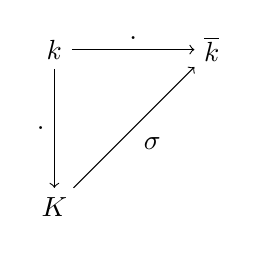
\begin{tikzpicture}[node distance=2cm, auto]
		\node (k) {$k$};
		\node (kk) [right of=k] {$\overline{k}$};
		\node (K) [below of=k] {$K$};

		\draw[->] (k) to node {$.$} (kk);
		\draw[->] (k) to node[swap] {$.$} (K);
		\draw[->] (K) to node[swap] {$\sigma$} (kk);

	\end{tikzpicture}
	\end{figure}

	\item $K$ é corpo de raízes sobre $k$ de uma família $(f_i)_{i \in I}$ de polinômios em $k[x] \setminus k$;
	\item Se $f \in k[x] \setminus k$ é irredutível em $k[x]$ com raiz $\alpha$, então $f(x)=c(x-\alpha_1)\cdots(x-\alpha_n)$ em $k[x]$, com $\alpha_1=\alpha$ e $c \in k \setminus \{0\}$.
	\end{enumerate}
\end{teo}
\begin{proof}
PULEI, tem nas notas mas não tudo.
\end{proof}

\begin{defi}
	Uma extensão de corpos $k \subseteq K$ é uma \emph{extensão normal} se ela satisfaz uma das três condições do teorema acima.
\end{defi}

OBS: Se $k \subseteq \overline{k}$ é uma extensão algébrica, então todo $\beta \in \overline{k}$ é algébrico sobre $k$ vale para $\beta \in K$, então $k \subseteq K$ é extensão algébrica.

	Se $k \subseteq K$ é extensão algébrica, então $k \subseteq K \subseteq \overline{K}$ são extensões algébricas, então $k \subseteq \overline{K}$ é extensão algébrica. Então $\overline{k} \sim \overline{K}$ é fecho algébrico de $k$.

(?????)

\begin{prop}
	Seja $k \subseteq K$ um extensão algébrica e $\sigma: K \to K$ um homomorfismo de cropos que satisfaz $\sigma|_k=id|_k$. Então $\sigma$ é um isomorfismo de corpos.
\end{prop}
\begin{proof}
...
\end{proof}

\begin{defi}
	Seja $E \subseteq F$ uma extensão algébrica e $\sigma:E \to L$ um homomorfismo de corpos tal que $L$ é algebricamente fechaado, $\sigma(E) \subseteq L$ é uma extensão algébrica ($L$ é fecho algébrico de $\sigma(E)$)
	\begin{equation*}
	S_\sigma \coloneqq \{\mu : \mu: F \to L \text{\ homomorfismo de corpos}, \mu|_E=\sigma\}.
	\end{equation*}
\end{defi}

\begin{lema}
	$|S_\sigma|$ depende de $E \subseteq F$, mas não depende de $\sigma$ nem de $L$.
\end{lema}
\begin{proof}
... vários diagramas
\end{proof}

\begin{defi}
	Seja $E \subseteq F$ uma extensão algébrica. O \emph{grau de separabilidade} da extensão é $[F:E]_S \coloneqq |S_\sigma|$. (Pode escolher $l=\overline{E}$ e $\sigma$ inclusão.)
\end{defi}

\begin{teo}
	\begin{enumerate}
	\item $E \subseteq F \subseteq K$ extensões algébricas, então
		\begin{equation*}
		[K:E]_S = [K:F]_S[F:E]_S
		\end{equation*}
	\item $E \subseteq F$ extensão finita (logo algébrica), então
		\begin{equation*}
		[F:E]_S \leq [F:E]
		\end{equation*}
	\end{enumerate}
\end{teo}
\begin{proof}
...
\end{proof}

\begin{defi}
	Seja $E \subseteq K$ uma extensão finita. Ela é \emph{separável} se $[K:E]_S=[K:E]$.
\end{defi}

\begin{coro}
	Sejam $E \subseteq F \subseteq K$ extensões de corpos, $[K:E] < \infty$, $E \subseteq K$ separável. Então $E \subseteq F$ e $F subseteq K$ são separáveis.
\end{coro}
\begin{proof}
	\begin{equation*}
	[K:F]_S [F:E]_S = [K:E]_S = [K:E] = [K:F][F:E].
	\end{equation*}
	Como $[F:E]_S \leq [F:E]$ e $[K:F]_S \leq [K:F]$, segue o corolário.
\end{proof}

























\newpage

\chapter{Matrizes}

\begin{defi}
	Seja $\bm A$ um anel e $l,c \in \N$. Uma \emph{matriz} de dimensão $l \times c$ sobre $\bm A$ é uma função $M: \inte_l \times \inte_c \to A$. Representa-se isso por
	\begin{equation*}
	M =
	\begin{bmatrix}
	m_{1,1} & \cdots & m_{1,c} \\
	\vdots & \ddots & \vdots \\
	m_{l,1} & \cdots & m_{l,c}
	\end{bmatrix},
	\end{equation*}
em que $m_{i,j} \coloneqq M(i,j) \in A$. O conjunto $\inte_l$ é o conjunto dos \emph{índices das linhas} e $\inte_c$ é o conjunto dos \emph{índices das colunas} da matriz $M$. A imagem de $M$ é o conjunto das \emph{entradas} da matriz $M$ e o elemento $m_{i,j}$ é a entrada da linha $i$ e coluna $j$.

	O conjunto de todas as matrizes de dimensão $l \times c$ sobre $\bm A$ é denotado por $\mathbb M_{l \times c}(\bm A)$.
\end{defi}

\begin{defi}
	Seja $\bm A$ um anel e $d \in \N$. Uma \emph{matriz quadrada} de dimensão $d$ sobre $\bm A$ é uma matriz $M \in \mathbb M_{d \times d}(\bm A)$. O conjunto de todas as matrizes quadradas de dimensão $d$ sobre $\bm A$ é denotado por $\mathbb M_d(\bm A)$.
\end{defi}

\begin{defi}
	Sejam $\bm A$ um anel e $M \in \mathbb M_{l \times c}(\bm A)$. A \emph{matriz transposta} de $M$ é a matriz $M^\intercal \in \mathbb M_{c \times l}(\bm A)$ definida por
	\begin{equation*}
	(M^\intercal)(i,j) \coloneqq m_{j,i}.
	\end{equation*}
\end{defi}

\section{Soma de Matrizes}

\begin{defi}
	Sejam $\bm A$ um anel e $M,N \in \mathbb M_{l \times c}(\bm A)$. A \emph{matriz soma} das matrizes $M$ e $N$ é a matriz $(M+N) \in \mathbb M_{l \times c}(\bm A)$ definida por
	\begin{equation*}
	(M+N)(i,j) \coloneqq m_{i,j}+n_{i,j}.
	\end{equation*}
\end{defi}

\begin{defi}
	Sejam $\bm A$ um anel e $0$ o elemento neutro da soma de $\bm A$.
	\begin{enumerate}
	\item A \emph{matriz nula} de dimensão $l \times c$ sobre $\bm A$ é a matriz $\zero_{l \times c} \in \mathbb M_{l \times c}(\bm A)$, definida por
		\begin{equation*}
		\zero_{l \times c}(i,j) \coloneqq 0.
		\end{equation*}
	\item Se $M \in \mathbb M_{l \times c}$, a \emph{matriz negativa} de $M$ é a matriz $-M \in \mathbb M_{l \times c}(\bm A)$, definida por
		\begin{equation*}
		(-M)(i,j) \coloneqq -m_{i,j}.
		\end{equation*}
	\end{enumerate}
\end{defi}

\begin{prop}
	Seja $\bm A$ um anel e $+$ a operação binária em $\mathbb M_{l \times c}(\bm A)$ definida por
	\begin{align*}
	+: \mathbb M_{l \times c}(\bm A) \times \mathbb M_{l \times c}(\bm A) &\to \mathbb M_{l \times c}(\bm A) \\
	(M,N) &\mapsto M+N.
	\end{align*}
Então $(\mathbb M_{l \times c}(\bm A),+)$ é um grupo com elemento neutro $\zero_{l \times c}$. Se $\bm A$ é comutativo, então $(\mathbb M_{l \times c}(\bm A),+)$ é comutativo.
\end{prop}
\begin{proof}
	Sejam $M,N,P \in \mathbb M_{l \times c}(\bm A)$. Primeiro, notemos que $+$ é associativa, pois, como a soma no anel é associativa, segue que
	\begin{equation*}
	(m_{i,j}+n_{i,j})+p_{i,j} = m_{i,j}+(n_{i,j}+p_{i,j})
	\end{equation*}
e, portanto, $(M+N)+P=M+(N+P)$. Então, notemos que $\zero$ é elemento neutro de $+$. Como $0$ é elemento neutro da soma da anel, segue que
	\begin{equation*}
	m_{i,j}+0 = 0+m_{i,j} = m_{i,j}
	\end{equation*}
e, portanto, $M+\zero=\zero+M=M$. Ainda, notemos que, como $-m_{i,j}$ é o inverso aditivo de $m_{i,j}$ no anel, segue que
	\begin{equation*}
	m_{i,j}+(-m_{i,j}) = (-m_{i,j})+m_{i,j} = 0
	\end{equation*}
e, portanto, $M+(-M)=(-M)+M=\zero$.	Assim, concluímos que $(\mathbb M_{l \times c}(\bm A),+)$ é um anel. Por fim, notemos que, se $\bm A$ é comutativo, então $+$ é comutativa, pois, como a soma no anel é comutativa, segue que
	\begin{equation*}
	m_{i,j}+n_{i,j} = n_{i,j}+m_{i,j}
	\end{equation*}
e, portanto, $M+N=N+M$. Assim, concluímos que, se $\bm A$ é comutativo, então $(\mathbb M_{l \times c}(\bm A),+)$ é comutativo.
\end{proof}

\section{Produto de Matrizes e Produto Por Escalar}

\begin{defi}
	Sejam $\bm A$ um anel e $M \in \mathbb M_{l \times d}(\bm A)$ e $N \in \mathbb M_{d \times c}(\bm A)$. A \emph{matriz produto} das matrizes $M$ e $N$ é a matriz $(MN) \in \mathbb M_{l \times c}(\bm A)$ definida por
	\begin{equation*}
	(MN)(i,j) \coloneqq \bigplus_{k=1}^d m_{i,k}n_{k,j}.
	\end{equation*}
\end{defi}

\begin{prop}
	Sejam $\bm A$ um anel e $M \in \mathbb M_{l \times d_1}(\bm A)$, $N \in \mathbb M_{d_1 \times d_2}(\bm A)$ e $P \in \mathbb M_{d_2 \times c}(\bm A)$. Então
	\begin{equation*}
	(MN)P = M(NP).
	\end{equation*}
\end{prop}
\begin{proof} Um elemento de $MN$ é dado por
	\begin{equation*}
	(mn)_{i,j} = \bigplus_{k_1=1}^{d_1} m_{i,k_1}n_{k_1,j}.
	\end{equation*}
Logo, um elemento de $(MN)P$ é dado por
	\begin{equation*}
	((mn)p)_{i,j} = \bigplus_{k_2=1}^{d_2} (mn)_{i,k_2}p_{k_2,j} = \bigplus_{k_2=1}^{d_2} \left(\bigplus_{k_1=1}^{d_1} m_{i,k_1}n_{k_1,k_2}\right)p_{k_2,j}.
	\end{equation*}
Analogamente, um elemento de $M(NP)$ é dado por
	\begin{equation*}
	(m(np))_{i,j} = \bigplus_{k_1=1}^{d_1} m_{i,k_1}(np)_{k_1,j} = \bigplus_{k_1=1}^{d_1} m_{i,k_1}\left(\bigplus_{k_2=1}^{d_2} n_{k_1,k_2}p_{k_2,j}\right).
	\end{equation*}
Mas então, como $\bm A$ é um anel, segue que
	\begin{align*}
	((mn)p)_{i,j}
	&= \bigplus_{k_2=1}^{d_2} \left(\bigplus_{k_1=1}^{d_1} m_{i,k_1}n_{k_1,k_2}\right)p_{k_2,j} \\
	&= \bigplus_{k_2=1}^{d_2} \left(\bigplus_{k_1=1}^{d_1} m_{i,k_1}n_{k_1,k_2}p_{k_2,j}\right) \\
	&= \bigplus_{k_1=1}^{d_1} \left(\bigplus_{k_2=1}^{d_2} m_{i,k_1}n_{k_1,k_2}p_{k_2,j}\right) \\
	&= \bigplus_{k_1=1}^{d_1} m_{i,k_1}\left(\bigplus_{k_2=1}^{d_2} n_{k_1,k_2}p_{k_2,j}\right) \\
	&= (m(np))_{i,j}.
	\end{align*}
\end{proof}

\begin{defi}
	Sejam $\bm A$ um anel e $0$ e $1$ os elementos neutros da soma e da multiplicação de $\bm A$ respectivamente. A \emph{matriz identidade} de dimensão $d$ sobre $\bm A$ é a matriz $\id_d \in \mathbb M_d(\bm A)$ definida por
	\begin{equation*}
	\id_d(i,j) \coloneqq \delta_{i,j} =
		\begin{cases}
			1 & i = j \\
			0 & i \neq j,
		\end{cases}
	\end{equation*}
\end{defi}

Essa função $\delta$ é conhecida como delta de Kronecker.

\begin{prop}
	Seja $\bm A$ um anel e $\cdot$ a operação binária em $\mathbb M_d(\bm A)$ definida por
	\begin{align*}
	\cdot: \mathbb M_d(\bm A) \times \mathbb M_d(\bm A) &\to \mathbb M_d(\bm A) \\
	(M,N) &\mapsto MN.
	\end{align*}
Então $(\mathbb M_d(\bm A),\cdot)$ é um monoide com elemento neutro $\id_d$.
\end{prop}
\begin{proof}
	Sejam $M,N,P \in \mathbb M_d(\bm A)$. Pela proposição anterior, sabemos que vale $(MN)P=M(NP)$ e que, portanto, $\cdot$ é associativa. Agora, notemos que um elemento de $M\id_d$ é da forma
	\begin{equation*}
	\bigplus_{k=1}^d m_{i,k}\delta_{k,j}.
	\end{equation*}
Mas, para $k \in \inte_d$, se $k \neq j$, então $\delta_{k,j}=0$ e, se $k=j$, então $\delta_{k,j}=1$ e, portanto, segue que
	\begin{equation*}
	\bigplus_{k=1}^d m_{i,k}\delta_{k,j} = m_{i,j}.
	\end{equation*}
Assim, concluímos que $M\id_d=M$. Analogamente, mostra-se que $\id_dM=M$, e concluímos que $\id_d$ é elemento neutro de $\cdot$. Isso mostra que $(\mathbb M_d(\bm A),\cdot)$ é um monoide.
\end{proof}

\begin{defi}
	Seja $\bm A$ um anel. Uma \emph{matriz invertível} é uma matriz $M \in \mathbb M_d(\bm A)$ que é invertível com respeito ao produto do monoide $(\mathbb M_d(\bm A),\cdot)$. A matriz inversa de $M$ é denotada $M^{-1}$.
\end{defi}

\begin{defi}
	Seja $\bm A$ um anel, $a \in A$ e $M \in \mathbb M_{l \times c}(\bm A)$. O \emph{produto por escalar} de $a$ e $M$ é a matriz $aM \in \mathbb M_{l \times c}$ definida por
	\begin{equation*}
	(aM)(i,j) \coloneqq am_{i,j}.
	\end{equation*}
\end{defi}

\section{Matrizes Quadradas}

\begin{defi}
	Seja $\bm A$ um anel.
	\begin{enumerate}
	\item Uma \emph{matriz triangular superior} é uma matriz quadrada $M \in \mathbb M_d(\bm A)$ que satisfaz
		\begin{equation*}
		\forall i,j \in \inte_d \qquad i > j \Rightarrow m_{i,j}=0.
		\end{equation*}
	\item Uma \emph{matriz triangular inferior} é uma matriz quadrada $M \in \mathbb M_d(\bm A)$ sobre $\bm A$ que satisfaz
		\begin{equation*}
		\forall i,j \in \inte_d \qquad i < j \Rightarrow m_{i,j}=0.
		\end{equation*}
	\item Uma \emph{matriz triangular superior} é uma matriz quadrada $M \in \mathbb M_d(\bm A)$ que satisfaz
		\begin{equation*}
		\forall i,j \in \inte_d \qquad i > j \Rightarrow m_{i,j}=0.
		\end{equation*}
	\item Uma \emph{matriz triangular} é uma matriz quadrada $M \in \mathbb M_d(\bm A)$ que é triangular superior ou triangular inferior.
	\item Uma \emph{matriz diagonal} é uma matriz quadrada $M \in \mathbb M_d(\bm A)$ que é triangular superior e triangular inferior; ou seja, que satisfaz
		\begin{equation*}
		\forall i,j \in \inte_d \qquad i \neq j \Rightarrow m_{i,j}=0.
		\end{equation*}
	\item Uma \emph{matriz simétrica}  uma matriz quadrada $M \in \mathbb M_d(\bm A)$ que é igual a sua transposta
		\begin{equation*}
		M = M^\intercal.
		\end{equation*}
	\item Uma \emph{matriz antissimétrica} é uma matriz quadrada $M \in \mathbb M_d(\bm A)$ que é igual à negativa da sua transposta
		\begin{equation*}
		M = -M^\intercal.
		\end{equation*}
	\item Uma \emph{matriz ortogonal} é uma matriz quadrada $M \in \mathbb M_d(\bm A)$ cuja transposta é igual à sua inversa
		\begin{equation*}
		M^\intercal = M^{-1}.
		\end{equation*}
	\end{enumerate}
\end{defi}

\section{Traço e Determinante}

\begin{defi}
	Sejam $\bm A$ um anel e $M \in \mathbb M_d(\bm A)$. O \emph{traço} de $M$ é o elemento $\tr(M) \in A$ definido por
	\begin{equation*}
	\tr(M) \coloneqq \bigplus_{i=1}^d m_{i,i}.
	\end{equation*}
\end{defi}

\begin{prop}
	Sejam $\bm A$ um anel, $a \in A$ e $M,N \in \mathbb M_d(\bm A)$. Então
	\begin{enumerate}
	\item $\tr(M^\intercal)=\tr(M)$;
	\item $\tr(MN)=\tr(NM)$;
	\item $\tr(M+N)=\tr(M)+\tr(N)$;
	\item $\tr(aM)=a\tr(M)$.
	\end{enumerate}
\end{prop}
\begin{proof}
	\begin{enumerate}
	\item
		\begin{equation*}
		\tr(M) = \bigplus_{i=1}^d m_{i,i} = \tr(M^\intercal).
		\end{equation*}
	\item
		\begin{align*}
		\tr(MN) &= \bigplus_{i=1}^d \left(\bigplus_{k=1}^d m_{i,k}n_{k,i}\right) \\
		&= \bigplus_{i=1}^d \left(\bigplus_{k=1}^d n_{k,i}m_{i,k}\right) \\
		&= \bigplus_{k=1}^d \left(\bigplus_{i=1}^d n_{k,i}m_{i,k}\right) \\
		&= \tr(NM).
		\end{align*}
	\item
		\begin{align*}
		\tr(M+N) &= \bigplus_{i=1}^d (m_{i,i} + n_{i,i}) \\
		&= \bigplus_{i=1}^d m_{i,i} + \bigplus_{i=1}^d n_{i,i} \\
		&= \tr(M) + \tr(N).
		\end{align*}
	\item
		\begin{equation*}
		\tr(aM) = \bigplus_{i=1}^d am_{i,i} = a\bigplus_{i=1}^d m_{i,i} = a\tr(M).
		\end{equation*}
\qedhere
	\end{enumerate}
\end{proof}














\chapter{Espaços Vetoriais}

\section{Espaço e Subespaço Vetoriais}

\begin{defi}
	Um \emph{espaço vetorial} (ou \emph{espaço linear}) sobre um corpo $\bm C=(C,+,\cdot)$ é uma tripla $\bm V = (V, \bm +, \bm \cdot)$ em que
	\begin{enumerate}
	\item $(V,\bm +)$ é um grupo comutativo com elemento neutro $\bm 0$;
	\item $\bm \cdot: C \times V \to V$ é uma função que satisfaz
		\begin{enumerate}
		\item $\forall \bm v \in V \qquad 1\bm\cdot \bm v=\bm v$;
		\item $\forall c_1,c_2 \in C \ \forall \bm v \in V \qquad (c_1 \cdot c_2) \bm\cdot \bm v = c_1 \bm\cdot(c_2 \bm\cdot \bm v)$;
		\end{enumerate}
	\item (Distributividades)
		\begin{enumerate}
		\item $\forall c \in C \ \forall \bm v_1,\bm v_2 \in V \qquad c \bm\cdot (\bm v_1 \bm + \bm v_2) = c \bm\cdot \bm v_1 \bm + c\bm\cdot \bm v_2$;
		\item $\forall c_1,c_2 \in C \ \forall \bm v \in V \qquad (c_1+c_2) \bm\cdot \bm v = c_1 \bm{\cdot v} \bm + c_2\bm{\cdot v}$.
		\end{enumerate}
	\end{enumerate}
Os elementos de $V$ são chamados de \emph{vetores} e denotados em negrito e os elementos de $C$ são chamados de \emph{escalares}. As operações $\bm +$ e $\bm \cdot$ são denotadas por $+$ e $\cdot$, o inverso de $\bm v \in V$ é denotado $- \bm v$ e a imagem de $(c,v) \in C \times V$, chamada de \emph{produto} de $c$ e $\bm v$, é denotada por $c\bm v$. Quando o corpo é $\R$, dizemos \emph{espaço vetorial real}, quando o corpo é $\C$, dizemos \emph{espaço vetorial complexo}.
\end{defi}

\begin{prop}
	Seja $\bm V$ um espaço vetorial sobre um corpo $\bm C$. Então, para todos $\bm v \in V$ e $c \in C$,
	\begin{enumerate}
	\item $c\bm v = \bm 0 \Leftrightarrow c=0 \ou \bm v = \bm 0$;
	\item $-(c\bm v) = (-c)\bm v = c(- \bm v)$;
	\item $c\bm v = (-c)(- \bm v)$.
	\end{enumerate}
\end{prop}
\begin{proof} Sejam $\bm v \in V$ e $c \in C$.
	\begin{enumerate}
	\item Primeiro, notemos que
		\begin{align*}
		0 \bm v &= 0 \bm v + \bm 0 \\
			&= 0 \bm v + (0 \bm v - 0 \bm v) \\
			&= (0 \bm v + 0 \bm v) - 0 \bm v \\
			&= (0+0) \bm v - 0 \bm v \\
			&= 0 \bm v - 0 \bm v \\
			&= \bm 0.
		  \end{align*}
Agora, notemos que
		\begin{align*}
		c \bm 0 &= c \bm 0 + \bm 0 \\
			&= c \bm 0 + (c \bm 0 - c \bm 0) \\
			&= (c \bm 0 + c \bm 0) - c \bm 0 \\
			&= c  (\bm 0 + \bm 0) - c \bm 0 \\
			&= c \bm 0 - c \bm 0 \\
			&= \bm 0.
		\end{align*}
Portanto, se $c=0$ ou $\bm v = \bm 0$, então $c\bm v = \bm 0$. Agora, suponhamos que $c\bm v =\bm 0$. Se $c \neq 0$, como $\bm C$ é corpo, segue da demonstração anterior que
		\begin{equation*}
		\bm v = c^{-1}c\bm v = c^{-1} \bm 0 = \bm 0.
		\end{equation*}
	\item Basta notar que
		\begin{align*}
		\bm -(c\bm{v}) &= \bm -(c\bm{v}) + \bm 0 \\
			&= \bm -(c\bm{v}) + (0 \bm v) \\
			&= \bm -(c\bm{v}) + (c-c) \bm v \\
			&= \bm -(c\bm{v}) + (c\bm v + (-c) \bm v) \\
			&= (\bm -(c\bm{v}) + c\bm v) + (-c) \bm v \\
			&= \bm 0 + (-c) \bm v \\
			&= (-c) \bm v
		\end{align*}
e que
		\begin{align*}
		-(c\bm{v}) &= -(c\bm{v}) + \bm 0 \\
			&= -(c\bm v) + (c \bm 0) \\
			&= -(c\bm v) + c(\bm v - \bm v) \\
			&= -(c\bm v) + (c\bm v + c(- \bm v)) \\
			&= (-(c\bm v + c\bm v) + c(- \bm v) \\
			&= \bm 0 + c(- \bm v) \\
			&= c(- \bm v).
		\end{align*}
	\item Do item anterior, segue que
		\begin{equation*}
		c\bm v = (-(-c))\bm v = (-c)(- \bm v).  \qedhere
		\end{equation*}
	\end{enumerate}
\end{proof}

\begin{prop}
	Seja $\bm C$ um corpo e $n$ um natural positivo. Então $(C^n,+,\bm\cdot)$, em que
	\begin{align*}
	\bm\cdot : C \times C^n &\to C^n \\
		(c,(c_1,\ldots,c_n)) &\mapsto (c \cdot c_1,\ldots,c \cdot c_n),
	\end{align*}
é um espaço vetorial sobre $\bm C$.
\end{prop}
\begin{proof}
	Claramente $(C^n,+)$ é um grupo comutativo com elemento neutro $(0,\ldots,0)$. Note que, para todos $(c_1,\ldots,c_n) \in C^n$ e $c,c' \in C$,
	\begin{equation*}
	1 \bm\cdot (c_1,\ldots,c_n) = (1 \cdot c_1,\ldots,1 \cdot c_n) = (c_1,\ldots,c_n)
	\end{equation*}
e
	\begin{align*}
	(c \cdot c') \bm\cdot (c_1,\ldots,c_n) &= ((c \cdot c') \cdot c_1, \ldots, (c \cdot c') \cdot c_n) \\
	&= ((c \cdot (c' \cdot c_1), \ldots, (c \cdot (c' \cdot c_n)) \\
	&= c \bm\cdot (c' \cdot c_1,\ldots,c' \cdot c_n) \\
	&= c \bm\cdot (c' \bm\cdot (c_1,\ldots,c_n)).
	\end{align*}
	Ainda, note que, para todos $(c_1,\ldots,c_n), (c'_1,\ldots,c'_n) \in C^n$ e $c,c' \in C$,
	\begin{align*}
	c \bm\cdot ((c_1,\ldots,c_n) + (c'_1,\ldots,c'_n)) &= c \bm\cdot (c_1+c'_1,\ldots,c_n+c'_n) \\
	&= (c \cdot (c_1+c'_1),\ldots,c \cdot (c_n+c'_n)) \\
	&= (c \cdot c_1 + c \cdot c'_1,\ldots,c \cdot c_n + c \cdot c'_n) \\
	&= (c \cdot c_1,\ldots,c \cdot c_n) + (c \cdot c'_1,\ldots,c \cdot c'_n) \\
	&= c \bm\cdot (c_1,\ldots,c_n) + c \bm\cdot (c'_1,\ldots,c'_n)
	\end{align*}
e
	\begin{align*}
	(c+c') \bm\cdot (c_1,\ldots,c_n) &= ((c+c')c_1,\ldots,(c+c')c_n) \\
	&= (c \cdot c_1 + c' \cdot c_1,\ldots,c \cdot c_n + c' \cdot c_n)_{i \in I} \\
	&= (c \cdot c_1,\ldots,c \cdot c_n) + (c' \cdot c_1,\ldots,c' \cdot c_n) \\
	&= c \bm\cdot (c_1,\ldots,c_n) + c' \bm\cdot (c_1,\ldots,c_n).  \qedhere
	\end{align*}
\end{proof}

Para generalizar esse resultado, lembremos que o produto de uma família $(C_i)_{i \in I}$ de conjuntos é $\bigtimes_{i \in I} C_i$ e, quando $C_i=C$, temos que $\bigtimes_{i \in I} C_i = C^I$ e os elementos de $C^I$ são funções $c=(c_i)_{i \in I}$ de $I$ em $C$.

\begin{prop}[EXERCÍCIO]
	Sejam $\bm C$ um corpo e $I$ um conjunto não vazio. Então $\bm {C^I}=(C^I,\bm +,\bm\cdot)$, em que
	\begin{align*}
	\bm + : C^I \times C^I &\to C^I \\
		(\bm c,\bm c') &\mapsto (c_i+c'_i)_{i \in I}
	\end{align*}
e
	\begin{align*}
	\bm\cdot : C \times C^I &\to C^I \\
		(a,\bm c) &\mapsto (a \cdot c_i)_{i \in I},
	\end{align*}
é um espaço vetorial sobre $\bm C$.
\end{prop}

\begin{prop}[Espaço de Funções]
	Sejam $\bm V$ e $\bm W$ espaços vetoriais sobre um corpo $\bm C$. Então $\bm{W^V}=(W^V,+,\cdot)$, em que
	\begin{align*}
	+: W^V \times W^V &\to W^V \\
		(\bm f_1,\bm f_2) &\mapsto \bm f_1+\bm f_2 : V \to W \\
										& \qquad \qquad \ \ \  \bm v \mapsto \bm f_1(\bm v)+\bm f_2(\bm v).
	\end{align*}
e
\begin{align*}
	\cdot: C \times W^V &\to W^V \\
		(c,\bm f) &\mapsto c\bm f : V \to W \\
										& \qquad \ \ \ \ \ \bm v \mapsto c\bm f(\bm v),
	\end{align*}
é um espaço vetorial sobre $\bm C$.
\end{prop}
\begin{proof}
	Primeiro, sabemos que $(W^V,+)$ é um grupo comutativo com elemento neutro $0: W^V \times W^V \to W^V$ definido por $0(\bm v)=0$. Devemos então mostrar que $\cdot: C \times W^V \to W^V$ satisfaz os itens da definição de espaço vetorial. Primeiro, seja $\bm f \in W^V$. Então, para todo $\bm v \in V$, $(1\bm f)(\bm v)=1\bm f(\bm v)=\bm f(\bm v)$, o que mostra que $1\bm f=\bm f$. Agora, sejam $c_1,c_2 \in C$ e $\bm f \in W^V$. Então, para todo $\bm v \in V$,
	\begin{equation*}
	((c_1c_2)\bm f)(\bm v) = (c_1c_2)\bm f(\bm v) = c_1(c_2\bm f(\bm v)) = c_1(c_2\bm f)(\bm v) = (c_1(c_2\bm f))(\bm v),
	\end{equation*}
o que mostra que $(c_1c_2)\bm f=c_1(c_2\bm f)$.

Por fim, devemos mostrar as propriedades distributivas. Sejam $c \in C$ e $\bm f_1,\bm f_2 \in W^V$. Então, para todo $\bm v \in V$,
	\begin{align*}
	(c(\bm f_1+\bm f_2))(\bm v)&=c(\bm f_1+\bm f_2)(\bm v) \\
	&=c(\bm f_1(\bm v)+\bm f_2(\bm v)) \\
	&= c\bm f_1(\bm v)+c \bm f_2(\bm v) \\
	&= (c\bm f_1)(\bm v)+(c \bm f_2)(\bm v) \\
	&=(c\bm f_1+c \bm f_2)(\bm v),
	\end{align*}
o que mostra que $c(\bm f_1+\bm f_2)=c\bm f_1+c \bm f_2$. Agora, sejam $c_1,c_2 \in C$ e $\bm f \in W^V$. Então, para todo $\bm v \in V$,
	\begin{align*}
	((c_1+c_2)\bm f)(\bm v) &= (c_1+c_2) \bm f(\bm v) \\
	&=c_1\bm f(\bm v)+c_2\bm f(\bm v) \\
	&=(c_1\bm f)(\bm v)+(c_2\bm f)(\bm v) \\
	&=(c_1\bm f+c_2\bm f)(\bm v),
	\end{align*}
o que mostra que $(c_1+c_2)\bm f=c_1\bm f+c_2\bm f$. Assim, concluímos que $(W^V,+,\cdot)$ é um espaço vetorial sobre $\bm C$.
\end{proof}

\begin{defi}
	Seja $\bm V$ um espaço vetorial sobre um corpo $\bm C$. Um \emph{subespaço vetorial} de $\bm V$ é um conjunto não vazio $W \subseteq V$ tal que
	\begin{enumerate}
	\item $\forall \bm w_1,\bm w_2 \in W \qquad \bm w_1 + \bm w_2 \in W$;
	\item $\forall c \in C \ \forall \bm w \in W \qquad c \bm w \in W$.
	\end{enumerate}
\end{defi}

\begin{prop}
	Seja $\bm V=(V,+,\cdot)$ um espaço vetorial sobre um corpo $\bm C$. Então um conjunto não vazio $W \subseteq V$ é um subespaço vetorial de $\bm V$ se, e somente se, $\bm W=(W,+|_{W \times W},\cdot|_{C \times W})$ é um espaço vetorial sobre $\bm C$.
\end{prop}
\begin{proof}
...
\end{proof}

\begin{prop}
	Seja $\bm V$ um espaço vetorial sobre um corpo $\bm C$ e $W$ um subespaço vetorial de $\bm V$. Então
	\begin{enumerate}
	\item $\bm 0 \in W$;
	\item $\{\bm 0\}$ e $V$ são subespaços vetoriais de $\bm V$.
	\end{enumerate}
\end{prop}
\begin{proof}
	\begin{enumerate}
	\item Como $W$ não é vazio, seja $\bm w \in W$. Então $0 \bm w = \bm 0 \in W$.
	\item Seja $W=\{\bm 0\}$. Se $\bm w_1,\bm w_2 \in W$, $\bm w_1 = \bm 0$ e $\bm w_2 =\bm 0$, e segue que $\bm w_1 + \bm w_2 = \bm 0 + \bm 0 = \bm 0$. Ainda, para todo $c \in C$, segue que $c\bm w_1 = c\bm 0=\bm 0 \in W$.
	Seja $W=V$. Como $\bm V$ é espaço vetorial, então $V$ é subespaço vetorial de $\bm V$ pala proposição anterior. \qedhere
	\end{enumerate}
\end{proof}

\begin{prop}
	Sejam $\bm V$ um espaço vetorial sobre um corpo $\bm C$ e $(W_i)_{i \in I}$ uma família de subespaços vetoriais de $\bm V$. Então
	\begin{equation*}
	W \coloneqq \bigcap_{i \in I} W_i
	\end{equation*}
é um subespaço vetorial de $\bm V$.
\end{prop}
\begin{proof}
	Como, para todo $i \in I$, $\bm 0 \in W_i$, segue que $\bm 0 \in W$ e, portanto, $W$ não é vazio. Agora, sejam $\bm w_1,\bm w_2 \in W$ e $c \in C$. Então, para todo $i \in I$, $\bm w_1,\bm w_2 \in W_i$ e, como $W_i$ é subespaço vetorial de $\bm V$, segue que $\bm w_1+\bm w_2 \in W_i$ e que $c\bm w_1 \in W_i$. Logo $\bm w_1+\bm w_2 \in W$ e $c\bm w_1 \in W$, o que mostra que $W$ é subespaço vetorial de $\bm V$.
\end{proof}

\begin{prop}
	Sejam $\bm V$ um espaço vetorial sobre um corpo $\bm C$ e $\{W_i\}_{i \in I}$ uma cadeia de subespaços vetoriais de $\bm V$ (ou seja, para todos $I,j \in I$, $W_I \subseteq W_j$ ou $W_j \subseteq W_i$). Então
	\begin{equation*}
	W \coloneqq \bigcup_{i \in I} W_i
	\end{equation*}
é um subespaço vetorial de $\bm V$.
\end{prop}
\begin{proof}
	Como, para todo $i \in I$, $\bm 0 \in W_i$, pois $W_i$ é subespaço vetoriasl de $\bm V$, segue que $\bm 0 \in W$ e, portanto, $W$ não é vazio. Agora, sejam $\bm w_1,\bm w_2 \in W$. Então existem $i,j \in I$ tais que $\bm w_1 \in W_i$ e $\bm w_2 \in W_j$. Nesse caso, $W_i \subseteq W_j$ ou $W_j \subseteq W_i$. Sem perda de generalidade, suponhamos o primeiro caso. Então segue que $\bm w_1 \in W_j$ e, portanto, $\bm w_1+\bm w_2 \in W_j$, o que mostra que $\bm w_1+\bm w_2 \in W$. Agora, seja $c \in C$ e notemos que, como $W_i$ é subespaço vetorial de $\bm V$, segue que $c\bm w_1 \in W_i$. Logo $c\bm w_1 \in W$, o que mostra que $W$ é subespaço vetorial de $\bm V$.
\end{proof}

\begin{defi}
	Sejam $\bm V$ um espaço vetorial sobre um corpo $\bm C$, $W \subseteq V$ e $(W_i)_{i \in I}$ uma indexação do conjunto de todos subespaços vetoriais de $\bm V$ dos quais $W$ é subconjunto. O \emph{subespaço vetorial gerado por $W$} em $\bm V$ é o subespaço vetorial
	\begin{equation*}
	\langle W \rangle \coloneqq \bigcap_{i \in I} W_i.
	\end{equation*}
Nesse caso, dizemos que $W$ é um \emph{conjunto gerador} de $\langle W \rangle$ ou que $W$ gera $\langle W \rangle$.

% Caso $W$ seja finito, $W = \{\bm w_1, \ldots, \bm w_n \}$, escrevemos $\langle W \rangle = \langle \bm w_1, \ldots, \bm w_n \rangle$.

\end{defi}

\begin{prop}
	Sejam $\bm V$ um espaço vetorial sobre um corpo $\bm C$. Então $\langle \emptyset \rangle = \{\bm 0\}$.
\end{prop}
\begin{proof}
	Como $\{\bm  0\}$ é um subespaço vetorial de $V$ e $\emptyset \subseteq \{\bm 0\}$, segue que, se $\bm v \in \langle \emptyset \rangle$, então $\bm v \in \{\bm 0\}$, o que implica $\bm v = \bm 0$ e, portanto, que $\langle \emptyset \rangle = \{\bm 0\}$.
\end{proof}

\section{Combinação Linear de Vetores}

\begin{defi}
	Sejam $\bm V$ um espaço vetorial sobre um corpo $\bm C$ e $W \subseteq V$ um conjunto finito tal que $W=\{\bm w_1,\ldots,\bm w_n\}$. Uma \emph{combinação linear} de $W$ em $\bm V$ é um vetor $\bm v \in V$ tal que existem $c_1,\ldots,c_n \in C$ satisfazendo
	\begin{equation*}
	\bm v = \bigplus_{i=1}^n c_i\bm w_i.
	\end{equation*}
Se $W$ é um conjunto infinito, uma \emph{combinação linear} de $W$ é uma combinação linear de um subconjunto finito de $W$.


\end{defi}

 O vetor $\bm 0$ é combinação linear de qualquer conjunto, pois é a soma vazia.

\begin{teo}
	Sejam $\bm V$ um espaço vetorial sobre um corpo $\bm C$ e $W \subseteq V$ não vazio. Então $\langle W \rangle$ é o conjunto de todas as combinações lineares de $W$ em $\bm V$.
\end{teo}
\begin{proof}
	Consideremos, primeiro, o caso em que $W=\emptyset$. Nesse caso, $\langle W \rangle = \{\bm 0\}$, e a única combinação linear de $W$ é a soma vazia $\bm 0$, o que mostra a igualdade dos conjuntos.

	Agora, assumamos que $W \neq \emptyset$ e seja $(W_j)_{j \in J}$ uma indexação do conjunto de todos subespaços de $\bm V$ que contêm $W$. Primeiro, mostraremos que uma combinação linear de $W$ em $\bm V$ está em $\langle W \rangle$. Seja $\bm v \coloneqq \bigplus_{i=1}^n c_i\bm w_i$ uma combinação linear de $W$ em $\bm V$. Para todo $j \in J$, $W_j$ é um subespaço vetorial de $\bm V$. Portanto, para todo $i \in \inte_n$, segue que $c_i \bm{w_i} \in W_j$ e, então, que $\bm v \in W_j$. Logo $\bm v \in \langle W \rangle$.

	Reciprocamente, mostraremos que o conjunto de todas combinações lineares de $W$ em $\bm V$ é um subespaço vetorial de $\bm V$. Primeiro, notemos que $\bm 0$ é uma combinação linear de $W$, pois, para todo $\bm w \in W$, vale $\bm 0 = 0\bm w$. Agora, sejam $\bm v_1 = \bigplus_{i=1}^n c_i\bm w_i$ e $\bm v_2 = \bigplus_{i=1}^m c'_i\bm w'_i$ combinações lineares de $W$ em $\bm V$ e $c \in C$. Então, se definirmos, para todo $i \in \inte_m$, $\bm w_{n+i} \coloneqq \bm w'_i$ e $c_{n+i} \coloneqq c'_i$ e, para todo $i \in \inte_n$, $\overline c_i \coloneqq cc_i$, segue que
	\begin{equation*}
	\bm v_1 + \bm v_2 = \bigplus_{i=1}^n c_i\bm w_i + \bigplus_{i=1}^m c'_i\bm w'_i = \bigplus_{i=1}^{n+m} c_i\bm w_i
	\end{equation*}
e
	\begin{equation*}
	c\bm v_1 = \bigplus_{i=1}^n (cc_i)\bm w_i = \bigplus_{i=1}^n \overline c_i \bm w_i
	\end{equation*}
são combinações lineares de $W$ em $\bm V$, o que implica que o conjunto de todas combinações lineares de $W$ em $\bm V$ é um subespaço de $\bm V$. Assim, como $\langle W \rangle$ é subconjunto de todo conjunto que é subespaço vetorial de $\bm V$ contendo $W$, segue que o conjunto de todas combinações lineares de $W$ em $\bm V$ é igual ao subespaço gerado por $W$.
\end{proof}

\begin{prop}
	Sejam $\bm V$ um espaço vetorial sobre um corpo $\bm C$, $W \subseteq V$ e $\bm v \in \langle W \rangle$. Então existem $\bm w_1, \ldots, \bm w_n \in W$ distintos e $c_1, \ldots, c_n \in C$ tais que
	\begin{equation*}
	\bm v = \bigplus_{i=1}^n c_i \bm w_i.
	\end{equation*}
\end{prop}
\begin{proof}
	Como $\bm v \in \langle W \rangle$, existem $\bm w'_1, \ldots, \bm w'_m \in W$ e $c'_1, \ldots, c'_m \in C$ tais que $\bm v = \bigplus_{i=1}^m c'_i \bm w'_i$. Vamos particionar o conjunto dos índices $\inte_m$ com a seguinte relação de equivalência: para todo $i,j \in \inte_m$, $i \sim j$ se, e somente se, $\bm w'_i = \bm w'_j$. Essa relação é de equivalência pois a igualddade de vetores é uma relação de equivalência. Agora, seja $n$ o número de classes de equivalências dessa relação. Para cada $i \in \inte_n$, seja $j \in P_i$ e definimos os vetores $\bm w_i \coloneqq \bm w'_j$. Notemos que os vetores $\bm w_i$ estão bem definidos, não dependem do $j$, pois, se $k \in P_i$, então $\bm w_i = \bm w'_j = \bm w'_k$. Ainda, definimos os coeficientes $c_i \coloneqq \bigplus _{j \in P_i} c'_j$. Desse modo, segue que
	\begin{equation*}
	\bm v = \bigplus_{i=1}^m c'_i \bm w'_i = \bigplus_{i=1}^n \bigplus_{j \in P_i} c'_j \bm w'_j = \bigplus_{i=1}^n \bigplus_{j \in P_i} c'_j \bm w_i =  \bigplus_{i=1}^n c_i \bm w_i.
	\end{equation*}
	Por fim, notemos que os $\bm w_1, \ldots, \bm w_n$ são distintos por definição, já que, se $\bm w_i = \bm w_j$ para $i,j \in \inte_n$, então existem $k,l \in \inte_m$ tais que $k \in P_i$, $l \in P_j$ e $\bm w_i = \bm w'_k$, $\bm w_j = \bm w'_l$. Mas isso implica $\bm w'_k=\bm w'_l$, o que implica $P_i = P_j$ e, portanto, $i = j$.
\end{proof}

\begin{defi}[Dependência Linear]
	Sejam $\bm V$ um espaço vetorial sobre um corpo $\bm C$ e $W \subseteq V$. Dizemos que $W$ é \emph{linarmente dependente} em $\bm V$ se existem $\bm w_1, \ldots,\bm w_n \in W$ distintos e $c_1,\ldots,c_n \in C$ não nulos tais que
	\begin{equation*}
	\bm 0 = \bigplus_{i=1}^n c_i \bm w_i.
	\end{equation*}
Caso contrário, dizemos que $W$ é \emph{linearmente independente} em $\bm V$.
\end{defi}

\begin{prop}
	Sejam $\bm V$ um espaço vetorial sobre um corpo $\bm C$ e $W \subseteq V$. Então $W$ é linearmente dependente se, e somente se, existe $\bm w \in W$ que é combinação linear de $W \setminus \{\bm w\}$ em $\bm V$.
\end{prop}
\begin{proof}
	Suponhamos que $W$ é linearmente dependente. Então existem vetores $\bm w'_1,\ldots,\bm w'_n \in W$ distintos e $c'_1,\ldots,c'_n \in C$ não nulos tais que
	\begin{equation*}
	\bm 0 = \bigplus_{i=1}^n c'_i \bm w'_i.
	\end{equation*}
Como $c'_1,\ldots,c'_n$ são não nulos, então existe $j \in \inte_n$ tal que $c'_j \neq 0$. Definindo $\bm w_i \coloneqq \bm w'_i$ se $1 \leq i < j$ e $\bm w_i \coloneqq \bm w'_{i-1}$ se $j < i \leq n$, e $c_i \coloneqq (c'_j)^{-1}(-c'_i)$ para todo $1 \leq i < j$ ou $j < i \leq n$, segue que
	\begin{equation*}
	\bm w'_j = \bigplus_{i=1}^{j-1} (c'_j)^{-1}(-c'_i) \bm w'_i + \bigplus_{i=j+1}^n (c'_j)^{-1}(-c'_i) \bm w'_i = \bigplus_{i=1}^{n-1} c_i \bm w_i.
	\end{equation*}
Por tanto, como $\bm w_i \in W \setminus \{\bm w'_j\}$ e $c_i \in C$ para todo $i \in \inte_{n-1}$, $\bm w'_j$ é combinação linear de $W \setminus \{\bm w'_j\}$ em $\bm V$.

	Reciprocamente, suponhamos que existe $\bm w \in W$ que é combinação linear de $W \setminus \{\bm w\}$ em $\bm V$. Então existem $\bm w_1, \ldots, \bm w_n \in W \setminus \{\bm w\}$ distintos e $c_1, \ldots, c_n \in C$ tais que
	\begin{equation*}
	\bm w = \bigplus_{i=1}^n c_i \bm w_i.
	\end{equation*}
Definindo $\bm w_{n+1} \coloneqq \bm w$ e $c_{n+1} \coloneqq -1$, segue que
	\begin{equation*}
	\bm 0 = \bigplus_{i=1}^n c_i \bm w_i - \bm w = \bigplus_{i=1}^{n+1} c_i \bm w_i.
	\end{equation*}
Então, como $\bm w_1, \ldots, \bm w_{n+1}$ são distintos e $c_{n+1} = -1 \neq 0$, segue que $W$ é linearmente dependente.
\end{proof}

\begin{prop}
	Sejam $\bm V$ um espaço vetorial sobre um corpo $\bm C$ e $W \subseteq V$. Então
	\begin{enumerate}
	\item $\emptyset$ é linearmente independente em $\bm V$;
	\item Se $\bm 0 \in W$, então $W$ é linearmente dependente em $\bm V$;
	\item Se $W=\{\bm v\}\neq\{\bm 0\}$, então $W$ é linearmente independente em $\bm V$.
	\end{enumerate}
\end{prop}
\begin{proof}
	\begin{enumerate}
	\item Suponha, por absurdo, que $\emptyset$ não é linearmente independente. Então existem $\bm{w_1},\ldots,\bm{w_n} \in \emptyset$ distintos e $c_1,\ldots,c_n \in C$ não nulos tais que
	\begin{equation*}
	\bm 0 = \bigplus_{i=1}^n c_i\bm{w_i}.
	\end{equation*}
Mas $\bm{w_1},\ldots,\bm{w_n} \in \emptyset$ é um absurdo.
	\item Seja $c \in C \setminus \{0\}$. Então, como $\bm 0 = c \bm 0$, segue que $W$ é linearmente dependente em $\bm V$.
	\item Se $\bm 0 = c\bm v$, como $\bm v \neq \bm 0$, segue que $c=0$, o que mostra que $W$ é linearmente independente em $\bm V$.
	\qedhere
	\end{enumerate}
\end{proof}

\begin{prop}
	Sejam $\bm V$ um espaço vetorial sobre um corpo $\bm C$ e $W \subseteq V$. Então $W$ é linearmente independente em $\bm V$ se, e somente se, para toda combinação linear $\bm v = \bigplus_{i=1}^n c_i\bm w_i \neq \bm 0$ de $W$ em $\bm V$ tal que $\bm w_1,\ldots,\bm w_n$ são distintos e não nulos, então $c_1,\ldots,c_n$ são únicos.
\end{prop}
\begin{proof}
	Primeiro, suponhamos que $W$ é linearmente dependente em $\bm V$. Então existem $\bm w'_1, \ldots,\bm w'_{n'} \in W$ distintos e $c'_1,\ldots,c'_{n'} \in C$ não nulos tais que
	\begin{equation*}
	\bm 0 = \bigplus_{i=1}^{n'} c'_i\bm w'_i.
	\end{equation*}
Nesse caso, seja $\bm v \in \langle W \rangle$. Se $\bm v = \bm 0$, então segue que









 .......................................... . Se $\bm v \neq \bm 0$










\end{proof}

\begin{prop}
	Sejam $\bm V$ um espaço vetorial sobre um corpo $\bm C$ e $\{W_i\}_{i \in I}$ uma cadeia de conjuntos linearmente independentes em $\bm V$ (ou seja, para todos $i,j \in I$, $W_i \subseteq W_j$ ou $W_j \subseteq W_i$). Então
	\begin{equation*}
	W \coloneqq \bigcup_{i \in I} W_i
	\end{equation*}
é um conjunto linearmente independente em $\bm V$.
\end{prop}
\begin{proof}
	Como, para todo $i \in I$, $\bm 0 \in W_i$, segue que $\bm 0 \in W$ e, portanto, $W$ não é vazio. Agora, sejam $\bm w_1,\bm w_2 \in W$. Então existem $i,j \in I$ tais que $\bm w_1 \in W_i$ e $\bm w_2 \in W_j$. Nesse caso, $W_i \subseteq W_j$ ou $W_j \subseteq W_i$. Sem perda de generalidade, suponhamos o primeiro caso. Então segue que $\bm w_1 \in W_j$ e, portanto, $\bm w_1+\bm w_2 \in W_j$, o que mostra que $\bm w_1+\bm w_2 \in W$. Agora, seja $c \in C$ e notemos que, como $W_i$ é subespaço vetorial de $\bm V$, segue que $c\bm w_1 \in W_i$. Logo $c\bm w_1 \in W$, o que mostra que $W$ é subespaço vetorial de $\bm V$.
\end{proof}


\section{Soma de Subespaços Vetoriais}

\begin{defi}
	Sejam $\bm V$ um espaço vetorial sobre um corpo $\bm C$ e $(W_i)_{i \in I}$ uma família de subespaços vetoriais de $\bm V$. A \emph{soma} de $(W_i)_{i \in I}$ é o subespaço vetorial gerado pela união de $W_i$. Denotamos
	\begin{equation*}
	\bigplus_{i \in I} W_i \coloneqq \left\langle \bigcup_{i \in I} W_i \right\rangle.
	\end{equation*}
Caso $(W_i)_{i \in I}$ seja uma família finita, escrevemos $W_1 + \cdots + W_n$.
\end{defi}

\begin{defi}
	Seja $\bm V$ um espaço vetorial sobre um corpo $\bm C$. Uma \emph{soma direta} é a soma de uma família $(W_i)_{i \in I}$ de subespaços vetoriais de $\bm V$ tal que $W_i \cap W_j = \{\bm 0\}$ para todo $i,j \in I$, $i \neq j$. Nesse caso, denotamos
	\begin{equation*}
	\bigoplus_{i \in I} W_i \coloneqq \left\langle \bigcup_{i \in I} W_i\right\rangle.
	\end{equation*}
Caso $(W_i)_{i \in I}$ seja uma família finita, escrevemos $W_1 \oplus \cdots \oplus W_n$.
\end{defi}

\begin{prop}
	Seja $\bm V$ um espaço vetorial sobre um corpo $\bm C$ e $W_1,\ldots,W_n$ subespaços vetoriais de $\bm V$ tais que $V = \bigplus_{i=1}^n W_i$. Então
	\begin{equation*}
	V=\bigoplus_{i=1}^n W_i
	\end{equation*}
se, e somente se, para todo $\bm v \in V$, existem únicos $\bm w_1 \in W_1,\ldots,\bm w_n \in W_n$ tais que
	\begin{equation*}
	\bm v = \bigplus_{i=1}^n \bm w_i.
	\end{equation*}
\end{prop}
\begin{proof}
	Mostraremos, primeiro, que se $V$ é soma direta de $W_1,\ldots,W_n$, então todo vetor de $V$ é soma única de vetores de $W_1,\ldots,W_n$. A demontração será por indução em $n$. O caso base é trivial, pois, se $V=W_1$, então, para todo $\bm v \in V$, $\bm v \in W_1$. Agora, suponhamos que a proposição vale para todo natural menor ou igual a $n$. Sejam $W_1,\ldots,W_{n+1}$ subespaços vetoriais de $V$ tais que $V = \bigplus_{i=1}^{n+1} W_i$. Então existem $\bm w_1 \in W_1,\ldots,\bm w_{n+1} \in W_{n+1}$ tais que
	\begin{equation*}
	\bm v = \bigplus_{i=1}^{n+1} \bm w_i.
	\end{equation*}
Suponhamos que existam $\bm w_1 \in W_1,\ldots,\bm w_{n+1} \in W_{n+1}$ tais que
	\begin{equation*}
	\bm v = \bigplus_{i=1}^{n+1} \bm w'_i.
	\end{equation*}
Então
	\begin{equation*}
	\bm v = \bigplus_{i=1}^{n+1} \bm w_i = \bigplus_{i=1}^{n+1} \bm w'_i,
	\end{equation*}
o que implica
	\begin{equation*}
	\bigplus_{i=1}^n (\bm w_i - \bm w'_i) = \bm w'_{n+1} - \bm w_{n+1}.
	\end{equation*}
Como, para todo $i \in \inte_{n+1}$, $w_i,w'_i \in W_i$, segue que $\bm w_i - \bm w'_i \in W_i$. Definamos $W \coloneqq \bigcup_{i=1}^n W_i$. Assim, segue que
	\begin{equation*}
	\bigplus_{i=1}^n (\bm w_i - \bm w'_i) \in \langle W \rangle
	\end{equation*}
e
	\begin{equation*}
	\bm w'_{n+1} - \bm w_{n+1} \in W_{n+1}.
	\end{equation*}
Ainda, como $V$ é soma direta de $W_1,\ldots,W_{n+1}$, então segue que $W \cap W_{n+1} = \{\bm 0\}$. Portanto concluímos que
	\begin{equation*}
	\bigplus_{i=1}^n (\bm w_i - \bm w'_i) = \bm w'_{n+1} - \bm w_{n+1} = \bm 0.
	\end{equation*}
Assim, concluímos que $\bm w'_{n+1}=\bm w_{n+1}$ e que
	\begin{equation*}
	\bigplus_{i=1}^n \bm w_i = \bigplus_{i=1}^n \bm w'_i.
	\end{equation*}
Mas notemos que
	\begin{equation*}
	\bm{\langle W \rangle}=(\langle W \rangle,+|_{\langle W \rangle \times \langle W \rangle},\cdot|_{\langle W \rangle \times \langle W \rangle})
	\end{equation*}
é um espaço vetorial e $W_1,\ldots,W_n$ são subespaços vetoriais de $\bm{\langle W \rangle}$ tais que $\langle W \rangle=\displaystyle\bigplus_{i=1}^n W_i$. Portanto, pela hipótese de indução, segue que, para todo $i \in \inte_n$, $\bm w_i = \bm w'_i$ e, portanto, concluímos que existem únicos $\bm w_1 \in W_1,\ldots,\bm w_{n+1} \in W_{n+1}$ tais que
	\begin{equation*}
	\bm v = \bigplus_{i=1}^{n+1} \bm w_i.
	\end{equation*}

	Suponhamos, então, que todo vetor de $V$ é soma de únicos vetores de $W_1$, $\ldots$, $W_n$. Sejam $i,j \in \inte_n$, $i \neq j$, e $\bm v \in W_i \cap W_j$. Como $\bm v \in V$, segue que existem únicos $\bm w_1 \in W_1, \ldots, \bm w_n \in W_n$ tais que
	\begin{equation*}
	\bm v = \bigplus_{k=1}^n \bm w_k.
	\end{equation*}
Sem perda de generalidade, suponhamos $i<j$. Notemos que
	\begin{equation*}
	\bm v = \bigplus_{i=1}^n \bm w_i = \bigplus_{k=1}^{i-1} \bm w_k + (\bm w_i+\bm v) +  \bigplus_{k=i+1}^{j-1} \bm w_k + (\bm w_j - \bm v) + \bigplus_{k=j+1}^n \bm w_k.
	\end{equation*}
Como $\bm v \in W_i \cap W_j$, segue que $(\bm w_i+\bm v) \in W_i$ e $(\bm w_j - \bm v) \in W_j$ e, portanto, como $\bm w_1 \in W_1, \ldots, \bm w_n \in W_n$ são únicos, segue que $(\bm w_i+\bm v) = \bm w_i$ e $(\bm w_j - \bm v) = \bm w_j$; ou seja, $\bm v = \bm 0$. Logo $V$ é soma direta de $W_1,\ldots,W_n$.
\end{proof}


\section{Bases de Espaços Vetoriais}

\begin{defi}
	Seja $\bm V$ um espaço vetorial sobre um corpo $\bm C$. Uma \emph{base} de $\bm V$ é um conjunto $B \subseteq V$ linearmente independente em $\bm V$ que gera $V$; ou seja, $V=\langle B \rangle$. Uma base de um subespaço vetorial $W$ de $\bm V$ é uma base do espaço vetorial $\bm W=(W,+|_{W \times W},\cdot|_{W \times W})$.
\end{defi}

\begin{teo}
	Sejam $\bm V$ um espaço vetorial sobre um corpo $\bm C$. Então existe base $B$ de $\bm V$ e, se $L$  é um conjunto linearmente independente em $\bm V$, existe uma base $B$ de $\bm V$ tal que $L \subseteq B$.
\end{teo}
\begin{proof}
	A afirmação de que todo espaço vetorial tem uma base é consequência da segunda afirmação porque, tomando $L=\emptyset$, sabemos que $L$ é linearmente independente e, portanto, existe base $B$ de $\bm V$ que contém $\emptyset$. Demonstraremos a segunda afirmação.

	Sejam $L$ um conjunto linearmente independente em $\bm V$ e $P$ o conjunto dos subconjuntos $S \subseteq V$ tais que $L \subseteq S$ e $S$ é linearmente independente em $\bm V$. Então $(P,\subseteq)$ é um conjunto parcialmente ordenado com a contenção de conjuntos usual. Agora, seja $(S_i)_{i \in I}$ uma cadeia de $(P,\subseteq)$. Consideremos o conjunto $S \coloneqq \bigcup_{i \in I} S_i$. Como $L \subseteq S_i$ para todo $i \in I$, então $L \subseteq S$. Devemos mostrar que $S$ é um conjunto linearmente independente em $\bm V$. Para isso, seja $M \subseteq S$ subconjunto finito de $S$. Como $(S_i)_{i \in I}$ é uma cadeia, existe $i \in I$ tal que $M \subseteq S_i$. Mas, como $S_i$ é linearmente independente, então $M$ também o é e, portanto, $S$ é linearmente independente. Logo $S$ é um limitante superior da cadeia. Concluímos, portanto, que existe um elemento maximal $B$ de $(P,\subseteq)$ que, por definição de $P$, é linearmente independente e $L \subseteq B$.

	Vamos mostrar que $B$ é base de $\bm V$. Devemos mostrar que $B$ gera $V$, ou seja, que $V=\langle B \rangle$.
Seja $\bm v \in V$ e suponhamos, por absurdo, que $\bm v \notin \langle B \rangle$. Então, em particular, $\bm v \notin B$; logo $B \subset B \cup \{\bm v\}$. Concluiremos que $B \cup \{\bm v\}$ é linearmente independente, o que constradiz a maximalidade de $B$. Seja $S$ um subconjunto finito de $B \cup \{\bm v\}$. Se $\bm v \notin S$, então $S \subseteq B$ e, portanto, é linearmente independente, pois $B$ o é; se $\bm v \in S$, sejam $\{\bm v_1,\ldots,\bm v_n\} \coloneqq S \setminus \{\bm v\} \subseteq B$ e $c,c_1,\ldots,c_n \in C$ tais que
	\begin{equation*}
	c_1\bm v_1 + \cdots + c_n\bm v_n -c\bm v=\bm 0.
	\end{equation*}
Como $\bm v \notin \langle B \rangle$, então $c=0$, pois, caso contrário, teríamos
	\begin{equation*}
	\bm v=\frac{c_1}{c}\bm v_1 + \cdots + \frac{c_n}{c}\bm v_n.
	\end{equation*}
Assim, segue que $c_1\bm v_1 + \cdots + c_n\bm v_n=\bm 0$. Mas $S \setminus \{\bm v\} \subseteq B$ é linearmente independente, pois $B$ o é, o que implica que $c_1=\cdots=c_n=0$ e, portanto, $S$ é linearmente independente. Com isso, concluímos que $B \cup \{\bm v\}$ é linearmente independente, pois todo subconjunto finito é, e isso contradiz a maximalidade de $B$. Por esse absurdo, segue que $\bm v \in \langle B \rangle$ e, portanto, que $V=\langle B \rangle$. Concluímos que $B$ é uma base de $\bm V$ que contém $L$.
\end{proof}

\begin{prop}
	Sejam $\bm V$ um espaço vetorial sobre um corpo $\bm C$ e $W,W' \subseteq V$ conjuntos finitos. Se $W$ é linearmente independente em $\bm V$ e $W'$ gera $V$, então $\card{W} \leq \card{W'}$.
\end{prop}
\begin{proof}
	Se $W=\emptyset$, então $0 = \card{W'} \leq \card{W}$. Caso contrário, seja $\card{W} = n$ e $(\bm w_i)_{i \in \inte_n}$ uma indexação de $W$. Suponhamos, por absurdo, que $W' = \emptyset$. Então, como $W'$ gera $V$ e $\langle W' \rangle = \{\bm 0\}$, segue que $V=\{\bm 0\}$, o que é absurdo, pois isso implica que $W=\{\bm 0\}$, que é um conjunto linearmente dependente. Então $W' \neq \emptyset$.  Seja $\card{W'} = m$ e $(\bm w'_i)_{i \in \inte_m}$ uma indexação de $W'$. Queremos mostrar que $n \leq m$. Suponhamos, por absurdo, que $m < n$. Como $W$ é linearmente independente, então, para todo $i \in \inte_n$, $\bm w_i \neq \bm 0$. Como $W'$ gera $V$, existem $c_1,\ldots,c_m \in C$ tais que
	\begin{equation*}
	\bm w_1 = \bigplus_{i=1}^m c_i \bm w'_i,
	\end{equation*}
e os $c_1,\ldots,c_m \in C$  não são todos nulos pois, caso contrário, teríamos $\bm w_1=\bm 0$. Assim, suponhamos,  sem perda de generalidade, que $c_1 \neq 0$. Então
	\begin{equation*}
	\bm w'_1 = c_1^{-1}\bm w_1 - \bigplus_{i=2}^m c_1^{-1}c_i \bm w'_i.
	\end{equation*}
Seja $W_1 \coloneqq \{\bm w_1,\bm w'_2,\ldots,\bm w'_m\}$. Como $W'$ gera $V$ e todo elemento de $W'$ pode ser escrito como combinação linear de $W_1$, $W_1$ gera $V$. Assim, analogamente, podemos escrever $\bm w_2$ como combinação linear de $W_1$, como $\bm w_2 \neq \bm 0$, segue que nem todo os coeficientes da combinação linear são nulos. Mais ainda, se somente o coeficiente de $\bm w_1$ é não nulo, então $\bm w_2$ é múltiplo de $\bm w_1$, o que contradiz a independência linear de $W$. Portanto, deve existir um coeficiente dos $\bm w'_2,\ldots,\bm w'_m$ não nulo. Assim, sem perda de generalidade, suponhamos que o coeficiente de $\bm w'_2$ é não nulo. Então, como no caso anterior, $\bm w'_2$ pode ser escrito como combinação linear de $\bm w_1, \bm w_2, \bm w'_3,\ldots, \bm w'_m$ e segue que o conjunto $W_2 \coloneqq \{\bm w_1, \bm w_2, \bm w'_3,\ldots, \bm w'_m\}$ gera $V$. Repetindo o processo, que termina porque $m<n$ são finitos, achamos o conjunto $W_m \coloneqq \{\bm w_1, \ldots, \bm w_m\}$, que gera $V$ e é um subconjunto próprio de $W$, pois $m < n$. Mas isso implica que $\bm w_{m+1} \in W$ é uma combinação linear de $W_m$ em $\bm V$, o que implica que $W$ é linearmente dependente, uma contradição. Logo $m \leq n$.
\end{proof}

\begin{teo}
	Sejam $\bm V$ um espaço vetorial sobre um corpo $\bm C$. Se $B,B' \subseteq V$ são bases de $\bm V$, então $\card{B} = \card{B'}$.
\end{teo}
\begin{proof}
	Primeiro, vamos mostrar que não ocorre o caso de uma base ser um conjunto finito e outra ser um conjunto infinito. Suponhamos, sem perda de generalidade, que $B$ é um conjunto finito com $\card{B}=n$, $\{\bm b_1,\ldots,\bm b_n\} \coloneqq B$, e $B'$ é um conjunto infinito. Seja $i \in \inte_n$. Como $\bm b_i \in V$ e $B'$ gera $V$, segue que existem $\bm b_{i,1}, \ldots, \bm b_{i,n_i} \in B'$ e $c_{i,1}, \ldots, c_{i,n_i} \in C$ tais que
	\begin{equation*}
	\bm b_i = \bigplus_{j=1}^{n_i} c_{i,j} \bm b_{i,j}.
	\end{equation*}
Notemos que o conjunto de todos esses $\bm b_{i,j}$ é $B'' \coloneqq \bigcup_{i=1}^n \{\bm b_{i,j} : j \in \inte_{n_i}\}$, que é um subconjunto finito de $B'$ e, portanto, um subconjunto próprio. Assim, como $B'' \subset B'$, existe $\bm b \in B' \setminus B''$. Como $\bm b \in V$ e $B$ é base, segue que existem $c_1, \ldots, c_n \in C$ tais que $\bm b = \bigplus_{i=1}^n c_i \bm b_i$. Mas então
	\begin{equation*}
	\bm b = \bigplus_{i=1}^n c_i \bm b_i = \bigplus _{i=1}^n c_i \bigplus_{j=1}^{n_i} c_{i,j} \bm b_{i,j} = \bigplus _{i=1}^n \bigplus_{j=1}^{n_i} c_ic_{i,j} \bm b_{i,j},
	\end{equation*}
o que mostra que $\bm b \in B'$ pode ser escrito como uma combinação linear de $B' \setminus \{\bm b\}$ em $\bm V$; ou seja, $B'$ não é linearmente independente, o que é um absurdo. Assim, existem dois casos a serem considereados; o primeiro em que ambas as bases são conjuntos finitos e o outro em que ambas são conjuntos infinitos.

	Suponhamos, no primeiro caso, que $B$ e $B'$ são conjuntos finitos com $\card{B}=n$ e $\card{B'}=m$. Como $B$ é linearmente independente e $B'$ gera $V$, segue que $\card{B} \leq \card{B'}$. Reciprocamente, como $B'$ é linearmente independente e $B$ gera $V$, segue que $\card{B'} \leq \card{B}$. Assim, segue que $\card{B} = \card{B'}$. Agora, suponhamos que $B$ e $B'$ são conjuntos infinitos.

TERMINAR
\end{proof}

\begin{defi}
	Sejam $\bm V$ um espaço vetorial sobre um corpo $\bm C$ e $B \subseteq V$ uma base $\bm V$. A \emph{dimensão} de $\bm V$ é o número ordinal
	$\dim \bm V \coloneqq \card{B}$.
\end{defi}

\section{Transformações Lineares}

\begin{defi}
	Sejam $\bm V$ e $\bm W$ espaços vetoriais sobre um corpo $\bm C$. Uma \emph{transformação linear} de $\bm V$ em $\bm W$ é uma função $T: V \to W$ que satisfaz
	\begin{enumerate}
	\item (Aditividade) $\forall \bm v_1,\bm v_2 \in V \qquad T(\bm v_1 + \bm v_2) = T(\bm v_1)+T(\bm v_2)$;
	\item (Homogeneidade) $\forall c \in C, \forall \bm v \in V \qquad T(c\bm v)=cT(\bm v)$.
	\end{enumerate}
O conjunto das transformações lineares de $\bm V$ em $\bm W$ é o conjunto $\lin(\bm V;\bm W)$ e o conjunto das tranformações lineares de $\bm V$ em $\bm V$ é o conjunto $\lin(\bm V) \coloneqq \lin(\bm V;\bm V)$.
\end{defi}

	É imediato da definição que as duas propriedades são equivalentes à seguinte propriedade
	\begin{equation*}
	\text{(Linearidade)}\ \forall c \in C, \forall \bm v_1,\bm v_2 \in V \qquad T(\bm v_1 + c\bm v_2) = T(\bm v_1)+cT(\bm v_2).
	\end{equation*}

\begin{prop}
	Sejam $\bm V$ e $\bm W$ espaços vetoriais sobre um corpo $\bm C$ e $T \in \lin(\bm V;\bm W)$. Então
	\begin{enumerate}
	\item (Linearidade generalizada) Para todos $\bm v_1,\ldots,\bm v_n \in V$ e $c_1,\ldots,c_n \in C$,
	\begin{equation*}
	T\left(\bigplus_{i=1}^n c_i \bm v_i \right) = \bigplus_{i=1}^n c_i T(\bm v_i).
	\end{equation*}

	\item $T(\bm 0) = \bm 0$;

	\item $T(-\bm v)=-T(\bm v)$.
\end{enumerate}
\end{prop}

\begin{prop}
	Sejam $\bm V$ e $\bm W$ espaços vetoriais sobre um corpo $\bm C$ e $T \in \lin(\bm V;\bm W)$. Então
\end{prop}

\begin{prop}
	Sejam $\bm V$ e $\bm W$ espaços vetoriais sobre um corpo $\bm C$. Então $\lin(\bm V;\bm W)$ é um subespaço vetorial de $\bm {W^V}$.
\end{prop}
\begin{proof}
	Primeiro, sejam $T_1,T_2 \in \lin(\bm V;\bm W)$. Então, para todos $c \in C$ e $\bm v_1,\bm v_2 \in V$,
	\begin{align*}
	(T_1+T_2)(\bm v_1+c\bm v_2)&=T_1(\bm v_1+c\bm v_2)+T_2(\bm v_1+c\bm v_2) \\
	&=T_1(\bm v_1)+cT_1(\bm v_2)+T_2(\bm v_1)+cT_2(\bm v_2) \\
	&=T_1(\bm v_1)+T_2(\bm v_1)+cT_1(\bm v_2)+cT_2(\bm v_2) \\
	&=(T_1+T_2)(\bm v_1)+c(T_1+T_2)(\bm v_2).
	\end{align*}
	Agora, sejam $c' \in C$ e $T \in \lin(\bm V;\bm W)$. Então
	\begin{align*}
	(c'T)(\bm v_1+c\bm v_2)&=c'T(\bm v_1+c\bm v_2) \\
	&=c'(T(\bm v_1)+cT(\bm v_2)) \\
	&= c'T(\bm v_1)+c'cT(\bm v_2) \\
	&= (c'T)(\bm v_1)+c(c'T)(\bm v_2).
	\end{align*}
Portanto concluímos que $\lin(\bm V;\bm W)$ é um subespaço vetorial de $\bm {W^V}$.
\end{proof}

\begin{prop}
	Sejam $\bm V_1$, $\bm V_2$ e $\bm V_3$ espaços vetoriais sobre um corpo $\bm C$. Se $T_1 \in \lin(\bm V_1;\bm V_2)$, $T_2 \in \lin(\bm V_2;\bm V_3)$, então $T_2 \circ T_1 \in \lin(\bm V_1; \bm V_3)$.
\end{prop}
\begin{proof}
	Sejam $c \in C$ e $\bm v_1,\bm v_2 \in V$. Então
	\begin{align*}
	(T_2 \circ T_1)(\bm v_1+c\bm v_2) &= T_2(T_1(\bm v_1+c\bm v_2)) \\
	&=T_2(T_1(\bm v_1)+cT_1(\bm v_2)) \\
	&=T_2(T_1(\bm v_1))+cT_2(T_1(\bm v_2)) \\
	&= (T_2 \circ T_1)(\bm v_1)+c(T_2 \circ T_1)(\bm v_2),
	\end{align*}
o que mostra que $T_2 \circ T_1$ é linear.
\end{proof}

\begin{prop}
	Sejam $\bm V$ e $\bm W$ espaços vetoriais sobre um corpo $\bm C$ e $T \in \lin(\bm V;\bm W)$. Se $T$ é invertível, então $T^{-1} \in \lin(\bm W;\bm V)$.
\end{prop}
\begin{proof}
	Seja $T \in \lin(\bm V;\bm W)$. Se $T$ é invertível, $T^{-1} \in V^W$ e, para todos $c \in C$ e $\bm w_1,\bm w_2 \in W$, existem $\bm v_1,\bm v_2 \in V$ tais que $T(\bm v_1)=\bm w_1$ e $T(\bm v_2)=\bm w_2$ e segue que
	\begin{align*}
	T^{-1}(\bm w_1+c\bm w_2)&=T^{-1}(T(\bm v_1)+cT(\bm v_2)) \\
	&= T^{-1}(T(\bm v_1+c\bm v_2)) \\
	&= \bm v_1+c\bm v_2 \\
	&= T^{-1}(\bm w_1)+cT^{-1}(\bm w_2),
	\end{align*}
o que mostra que $T^{-1}$ é linear.
\end{proof}

\begin{prop}
	Sejam $\bm V$ e $\bm W$ espaços vetoriais sobre um corpo $\bm C$, $B_V=\{\bm v_1,\ldots,\bm v_n\}$ base de $\bm V$, $B_W=\{\bm w_1,\ldots,\bm w_m\}$ base de $\bm W$ e $T \in \lin(\bm V;\bm W)$. Então, para todo $\bm v \in V$, existem únicos $c_1,\ldots,c_m \in C$ tais que
	\begin{equation*}
	T(\bm v) = \bigplus_{i=1}^m c_j \bm w_j.
	\end{equation*}
\end{prop}
\begin{proof}
	Primeiro demonstraremos a existência. Sabemos que, como $B_V$ é base de $V$, então existem únicos $a_1,\ldots,a_n \in C$ tais que $\bm v = \bigplus_{i=1}^n a_i\bm v_i$. Mas, como $T$ é linear, então
	\begin{equation*}
	T(\bm v) = T\left( \bigplus_{i=1}^n a_i \bm v_i \right) = \bigplus_{i=1}^n a_i T(\bm v_i).
	\end{equation*}
	Agora, como $B_W$ é base de $\bm W$, para cada $i \in \{1,\ldots,n\}$ existem únicos
	\begin{equation*}
	b_{i1},\ldots,b_{im} \in C
	\end{equation*}
tais que  $T(\bm v_i)=\bigplus_{j=1}^m b_{ij} \bm w_j$. Assim, definindo $c_j \coloneqq \bigplus_{i=1}^n a_i b_{ij}$, segue que
	\begin{equation*}
	T(\bm v)=\bigplus_{i=1}^n a_i \left(\bigplus_{j=1}^m b_{ij} \bm w_j \right) = \bigplus_{j=1}^m \left(\bigplus_{i=1}^n a_i b_{ij}\right) \bm w_j = \bigplus_{j=1}^m c_j \bm w_j.
	\end{equation*}

\end{proof}

\section{Espaços Vetoriais Normados}

\begin{defi}
	Seja $\bm V$ um espaço vetorial real. Uma \emph{norma em $\bm V$} é uma função $\nor{\cdot}: V \to \R$ tal que
	\begin{enumerate}
	\item $\forall \bm v \in V, \forall c \in \R \qquad \nor{c \bm v} = |c|\nor{\bm v}$;
	\item $\forall \bm v_1, \bm v_2 \in V \qquad \nor{\bm v_1 + \bm v_2} \leq \nor{\bm v_1} + \nor{\bm v_2}$;
	\item $\nor{\bm v} = 0 \Rightarrow \bm v = \bm 0$.
	\end{enumerate}
\end{defi}

\begin{prop}
	Sejam $\bm V$ um espaço vetorial real e $\nor{\cdot}$ uma norma em $\bm V$. Então
	\begin{enumerate}
	\item $\nor{\bm 0} = 0$
	\item $\nor{- \bm v} = \nor{\bm v}$
	\item $\forall \bm v \in V \qquad 0 \leq \nor{\bm v}$.
	\end{enumerate}
\end{prop}

\cleardoublepage
\section{Produto e Coproduto de Espaços Vetoriais}

\subsection{Produto}

\begin{defi}
Seja $(\bm{V_i})_{i \in I} = ((V_i,+_i,\cdot_i))_{i \in I}$ uma família de espaços vetoriais sobre um corpo $\bm C$. O \emph{produto categórico} de $(\bm{V_i})_{i \in I}$ é a tripla
	\begin{equation*}
	\prod_{i \in I} \bm{V_i} = (V,+,\cdot),
	\end{equation*}
em que $V = \prod_{i \in I} V_i$,
	\begin{align*}
	+: V \times V &\to V \\
			(v_1,v_2) &\mapsto ((v_1)_i +_i (v_2)_i)_{i \in I}
	\end{align*}
e
	\begin{align*}
	\cdot: C \times V &\to V \\
			(c,v) &\mapsto (c \cdot_i v_i)_{i \in I}.
	\end{align*}
\end{defi}

\begin{prop}
Seja $(\bm{V_i})_{i \in I} = ((V_i,+_i,\cdot_i))_{i \in I}$ uma família de espaços vetoriais sobre um corpo $\bm C$. Então $\prod_{i \in I} \bm{V_i} = (V,+,\cdot)$ é um espaço vetorial sobre $\bm C$.
\end{prop}
\begin{proof}
	\begin{enumerate}
	\item $(V,+)$ é um grupo pois tem a mesma operação do produto de grupos (\ref{alge:prop.gru.prod}).
	
	\item Seja $v \in V$. Então
	\begin{equation*}
	1v = (1v_i)_{i \in I} = (v_i)_{i \in I} = v.
	\end{equation*}
	Sejam $c_1,c_2 \in C$ e $v \in V$. Então
	\begin{align*}
	(c_1c_2)v &= ((c_1c_2)v_i)_{i \in I} \\
		&= (c_1(c_2v_i))_{i \in I} \\
		&= c_1(c_2v_i)_{i \in I} \\
		&= c_1(c_2v).
	\end{align*}
	
	\item (Distributividades) Sejam $c \in C$ e $v,v' \in V$. Então
	\begin{align*}
	c(v+v') &= c(v_i+v'_i)_{i \in I} \\
		&= (c(v_i+v'_i))_{i \in I} \\
		&= (cv_i + cv'_i)_{i \in I} \\
		&= (cv_i)_{i \in I} + (cv'_i)_{i \in I} \\
		&= cv+cv'.
	\end{align*}
	Sejam $c_1,c_2 \in C$ e $v \in V$. Então
	\begin{align*}
	(c_1+c_2)v &= ((c_1+c_2)v_i)_{i \in I} \\
		&= (c_1v_i+c_2v_i)_{i \in I} \\
		&= (c_1v_i)_{i \in I} + (c_2v_i)_{i \in I} \\
		&= c_1v+c_2v. \qedhere
	\end{align*}
	\end{enumerate}
\end{proof}

\begin{prop}
Seja $(\bm{V_i})_{i \in I} = ((V_i,+_i,\cdot_i))_{i \in I}$ uma família de espaços vetoriais sobre um corpo $\bm C$. Para todo $i \in I$, a projeção canônica $\pi_i: \prod_{i \in I} \bm{V_i} \to \bm{V_i}$ é uma transformação linear.
\end{prop}
\begin{proof} Sejam $c \in C$ e $v,v' \in \prod_{i \in I} V_i$. Então
	\begin{equation*}
	\pi_i(v+cv') = \pi_i ((v_i+cv'_i)_{i \in I}) = v_i+cv'_i = \pi_i(v) + c\pi_i(v'). \qedhere
	\end{equation*}
\end{proof}

\begin{prop}[Propriedade Universal]
Sejam $(\bm{V_i})_{i \in I}$ uma família de espaços vetoriais sobre um corpo $\bm C$, $\bm X$ um espaço vetorial sobre $\bm C$ e, para todo $i \in I$, $L_i: \bm X \to \bm{V_i}$ uma transformação linear. Então existe única transformação linear $L: \bm X \to \prod_{i \in I} \bm{V_i}$ tal que, para todo $i \in I$, $\pi_i \circ L = L_i$ (o diagrama comuta).
\begin{figure}
\centering
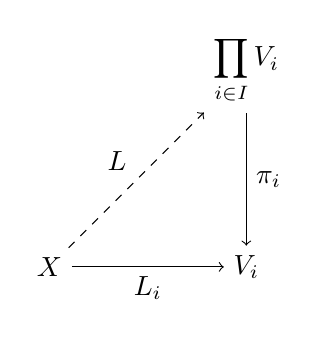
\begin{tikzpicture}[node distance=2.5cm, auto]
	\node (P) {$\displaystyle\prod_{i \in I} \bm{V_i}$};
	\node (Ci) [below of=P] {$\bm{V_i}$};
	\node (X) [left of=Ci] {$\bm X$};
	\draw[->] (X) to node [swap] {$L_i$} (Ci);
	\draw[->, dashed] (X) to node {$L$} (P);
	\draw[->] (P) to node {$\pi_i$} (Ci);
\end{tikzpicture}
\end{figure}
\end{prop}
\begin{proof}
Defina a função
	\begin{align*}
	\func{L}{X}{\prod_{i \in I} V_i}{x}{(L_i(x))_{i \in I}}.
	\end{align*}
Da propriedade universal para conjuntos, $L$ é a única função de $X$ para $\bigtimes_{i \in I} \bm{V_i}$ tal que, para todo $i \in I$, $\pi_i \circ L = L_i$. Falta mostrar que $L$ é transformação linear. Sejam $c \in C$ e $x_1,x_2 \in V$. Então
	\begin{align*}
	L(x_1+cx_2) &= (L_i(x_1+cx_2))_{i \in I} \\
		&= (L_i(x_1)+cL_i(x_2))_{i \in I} \\
		&= (L_i(x_1))_{i \in I}+c(L_i(x_2))_{i \in I} \\
		&= L(x_1)+cL(x_2). \qedhere
	\end{align*}
\end{proof}

\subsection{Coproduto (Soma)}

\begin{defi}
Seja $(\bm{V_i})_{i \in I} = ((V_i,+_i,\cdot_i))_{i \in I}$ uma família de espaços vetoriais. A \emph{soma categórica} de $(\bm{V_i})_{i \in I}$ é
	\begin{equation*}
	\coprod_{i \in I} \bm{V_i} = (V,+,\cdot),
	\end{equation*}
em que $V = \set{(v_i)_{i \in I} \in \prod_{i \in I} V_i}{\exists J \subseteq I \qquad \card{J} < \card{\N} \e v_i \neq 0}$,
	\begin{align*}
	+: V \times V &\to V \\
			(v_1,v_2) &\mapsto ((v_1)_i +_i (v_2)_i)_{i \in I}
	\end{align*}
e
	\begin{align*}
	\cdot: C \times V &\to V \\
			(c,v) &\mapsto (c(v)_i)_{i \in I}.
	\end{align*}
\end{defi}

Observe que, se $\card{I} < \card{\N}$, então $\prod_{i \in I} \bm{V_i} = \coprod_{i \in I} \bm{V_i}$.

\begin{prop}[Propriedade Universal]
Sejam $(\bm{V_i})_{i \in I}$ uma família de espaços vetoriais sobre um corpo $\bm C$, $\bm X$ um espaço vetorial sobre $\bm C$ e, para todo $i \in I$, $L_i: \bm{V_i} \to \bm X$ uma transformação linear. Então existe única transformação linear $L: \bm X \to \coprod_{i \in I} \bm{V_i}$ tal que, para todo $i \in I$, $L \circ \iota_i = L_i$ (o diagrama comuta).
\begin{figure}
\centering
\begin{tikzpicture}[node distance=2.5cm, auto]
	\node (Ci) {$\bm{V_i}$};
	\node (S) [below of=Ci] {$\displaystyle\coprod_{i \in I} \bm{V_i}$};
	\node (X) [right of=Ci] {$\bm X$};
	\draw[->] (Ci) to node {$L_i$} (X);
	\draw[->, dashed] (S) to node [swap] {$L$} (X);
	\draw[->] (Ci) to node [swap] {$\iota_i$} (S);
\end{tikzpicture}
\end{figure}
\end{prop}

O coproduto de espaços vetoriais é também chamado de \emph{soma} ou \emph{soma direta} e denotado
	\begin{equation*}
	\bigoplus_{i \in I} \bm{V_i}.
	\end{equation*}


























\chapter{Álgebra Multilinear}

\section{Transformações Multilineares}

\begin{defi}
Sejam $\bm{V_0},\cdots,\bm{V_{n-1}}$ e $\bm W$ espaços lineares sobre um corpo $\bm C$. Uma \emph{transformação $n$-linear} de $(\bm{V_0},\ldots,\bm{V_{n-1}})$ para $\bm W$ é uma função
	\begin{equation*}
	T: \bm V_0 \times \cdots \times \bm V_{n-1} \to \bm W
	\end{equation*}
tal que, para todo $0 \leq i < n$ e $(\bm v_0,\ldots,\bm v_{i-1},\bm v_{i+1},\ldots,\bm v_{n-1}) \in \bm{V_0} \times \cdots \times \bm{V_{i-1}} \times \bm{V_{i+1}} \times \cdots \times \bm V_{n-1}$, a função
	\begin{align*}
	\func{T(\bm v_0,\ldots,\bm v_{i-1},\var,\bm v_{i+1},\ldots,\bm v_{n-1})}{\bm{V_i}}{\bm W}{\bm v}{T(\bm v_0,\ldots,\bm v_{i-1},\bm v,\bm v_{i+1},\ldots,\bm v_{n-1})}
	\end{align*}
%	\begin{align*}
%	\func{T(\bm v_0,\ldots,\underbrace{\var}_i,\ldots,\bm v_{n-1})}{\bm{V_i}}{\bm W}{\bm v}{T(\bm v_0,\ldots,\underbrace{\bm v}_i,\ldots,\bm v_{n-1})}
%	\end{align*}
é uma transformação linear. O conjunto dessas transformações é denotado
	\begin{equation*}
	\lin(\bm{V_0},\ldots,\bm{V_{n-1}};\bm W)
	\end{equation*}
e, quando todos os espaços $\bm{V_i}$ são iguais, denota-se
	\begin{equation*}
	\lin^n(\bm V;\bm W) \coloneqq \lin(\underbrace{\bm V,\ldots,\bm V}_n;\bm W)
	\end{equation*}
\end{defi}

\begin{prop}
Sejam $\bm{V_0},\cdots,\bm{V_{n-1}}$ e $\bm W$ espaços lineares de dimensão finita sobre um corpo $\bm C$ cujas dimensões são $d_0,\ldots,d_{n-1}$ e $d$, respectivamente, e, para cada $i \in n$, seja $(\bm b_{ij})_{j \in d_i}$ uma base ordenada de $\bm{V_i}$. Então toda transformação $n$-linear $T \in \lin(\bm{V_0},\ldots,\bm{V_{n-1}};\bm W)$ está determinada pelos seus valores em $(\bm b_{0j_0},\ldots,\bm b_{(n-1)j_{n-1}})$.
\end{prop}
\begin{proof}
Como consequência da propriedade de linearidade generalizada para transformações lineares, para todos $\bm v_0,\ldots,\bm v_{m-1} \in \bm{V_k}$ e $c_0,\ldots,c_{m-1} \in C$, vale que
	\begin{equation*}
	T\left(\bm v_0,\ldots,\bigplus_{i \in m} c_i\bm v_i,\ldots,\bm v_{n-1} \right) = \bigplus_{i \in m} c_iT\left(\bm v_0,\ldots,\bm v_i,\ldots,\bm v_{n-1} \right).
	\end{equation*}
Sendo assim, para cada $i \in n$, sejam $\bm v_i \in \bm{V_i}$ e $v_{i0},\ldots,v_{id_i} \in C$ os coeficientes de $\bm v_i$ na base $\bm b_i$, de modo que
	\begin{equation*}
	\bm v_i = \bigplus_{j \in d_i} v_{ij} \bm b_{ij}.
	\end{equation*}
Pela linearidade em cada entrada, temos que
	\begin{align*}
	T(\bm v_0,\ldots,\bm v_{n-1}) &= T\left(\bigplus_{j_0 \in d_0} v_{0j} \bm b_{0j_0},\ldots,\bigplus_{j_{n-1} \in d_{n-1}} v_{(n-1)j_{n-1}} \bm b_{(n-1)j_{n-1}} \right) \\
		&= \bigplus_{j_0 \in d_0} \cdots \bigplus_{j_{n-1} \in d_{n-1}} v_{0j_0} \cdots v_{(n-1)j_{n-1}} T\left(\bm b_{0j_0},\ldots,\bm b_{(n-1)j_{n-1}} \right) \\
		&= \bigplus_{(j_0,\ldots,j_{n-1}) \in d_0 \times \cdots \times d_{n-1}} v_{0j_0} \cdots v_{(n-1)j_{n-1}} T\left(\bm b_{0j_0},\ldots,\bm b_{(n-1)j_{n-1}} \right). 
	\end{align*}
Portanto a função $T$ está determinada pelos valores que tem nos elementos
	\begin{equation*}
	(\bm b_{0j_0},\ldots,\bm b_{(n-1)j_{n-1}}).
	\end{equation*}
Como há $d_0 \cdots d_{n-1}$ desses elementos, há essa quantidade de escolhas a serem determinadas para se determinar os valores de $T$.
\end{proof}

\begin{prop}
Sejam $\bm{V_1},\cdots,\bm{V_n}$ e $\bm W$ espaços lineares sobre um corpo $\bm C$. Então
	\begin{equation*}
	\bm{\lin(\bm{V_1},\ldots,\bm{V_n};\bm W)} \coloneqq (\lin(\bm{V_1},\ldots,\bm{V_n};\bm W),+,\cdot),
	\end{equation*}	
em que $+$ e $\cdot$ são a soma e o produto escalar pontuais induzidos por $\bm W$, é um espaço linear sobre $\bm C$ (de dimensão ...).
\end{prop}

\section{Formas Multilineares}

\begin{defi}
Seja $\bm V$ um espaço linear sobre um corpo $\bm C$. Uma \emph{forma $k$-linear} em $\bm V$ é uma função $f \in \lin^k(\bm V;\bm C)$, ou seja, um funcional $k$-linear em $(\bm V,\ldots,\bm V)$.
\end{defi}

\begin{defi}
Seja $\bm V$ um espaço linear sobre um corpo $\bm C$. Uma forma $k$-linear $f$ em $\bm V$ é:
\begin{enumerate}
\item \emph{simétrica} se, e somente se, para toda permutação $p \in \sime_k$ e todos $\bm v_0$, $\ldots$, $\bm v_{k-1} \in V$,
	\begin{equation*}
	f(\bm v_{p(0)},\ldots,\bm v_{p(k-1)}) = f(\bm v_0,\ldots,\bm v_{k-1});
	\end{equation*}
\item \emph{antissimétrica} se, e somente se, para toda permutação $p \in \sime_k$ e todos $\bm v_0,\ldots,\bm v_{k-1} \in V$,
	\begin{equation*}
	f(\bm v_{p(0)},\ldots,\bm v_{p(k-1)}) = \prd(p) f(\bm v_0,\ldots,\bm v_{k-1});
	\end{equation*}
\item \emph{alternada} se, e somente se, para todos $\bm v_0,\ldots,\bm v_{k-1} \in V$ linearmente dependentes,
	\begin{equation*}
	f(\bm v_0,\ldots,\bm v_{k-1}) = 0.
	\end{equation*}
\end{enumerate}
O conjunto das formas $k$-lineares alternadas é denotado $\mathcal A^k(\bm V)$.
\end{defi}

\begin{prop}
Sejam $\bm V$ um espaço linear sobre um corpo $\bm C$ e $f \in \lin^k(\bm V;\bm C)$.
\end{prop}

\begin{prop}
Seja $\bm V$ um espaço linear sobre um corpo $\bm C$. Então
\begin{enumerate}
\item Uma forma $k$-linear em $\bm V$ é alternada se, e somente se, para todos $\bm v_0$, $\ldots$, $\bm v_{k-1} \in V$ tais que $\bm v_i = \bm v_j$ para dois $i,j \in k$ distintos,
	\begin{equation*}
	f(\bm v_0,\ldots,\bm v_{k-1})=0.
	\end{equation*} 
\item Uma forma alternada $k$-linear em $\bm V$ é antissimétrica. Se a característica de $\bm C$ é diferente de $2$, então uma forma antissimétrica $k$-linear em $\bm V$  é alternada.
\item Se a característica de $\bm C$ é igual a $2$, então uma forma $k$-linear em $\bm V$ é antissimétrica se, e somente se, é simétrica.
\end{enumerate}
\end{prop}
\begin{proof}
\begin{enumerate}
\item Se $f$ é alternada, então, para todos $\bm v_0,\ldots,\bm v_{k-1} \in V$ tais que $\bm v_i = \bm v_j$ para dois $i,j \in k$ distintos, o conjunto $\{\bm v_0,\ldots,\bm v_{k-1}\}$ é linearmente dependente, portanto $f(\bm v_0,\ldots,\bm v_{k-1})=0$. Reciprocamente, suponha que $f$ satisfaz a propriedade e sejam $\bm v_0,\ldots,\bm v_{k-1} \in V$ linearmente dependentes. Então existe $i \in k$ tal que $\bm v_i$ é combinação linear dos outros $\bm v_j$: existem $c_j \in C$, $j \in k\setminus\{i\}$, tais que
	\begin{equation*}
	\bm v_i = \bigplus_{j \in k\setminus\{i\}} c_j \bm v_j.
	\end{equation*}
Assim, segue da $k$-linearidade e da propriedade que
	\begin{align*}
	f(\bm v_0,\ldots,\bm v_{k-1}) &= f\left(\bm v_0,\ldots, \bigplus_{j \in k\setminus\{i\}} c_j \bm v_j,\ldots,\bm v_{k-1}\right) \\
		&= \bigplus_{j \in k\setminus\{i\}} c_j f(\bm v_0,\ldots, \bm v_j,\ldots,\bm v_{k-1}) \\
		&=\bigplus_{j \in k\setminus\{i\}} c_j 0 = 0.
	\end{align*}

\item Suponha $f$ alternada e sejam $\bm v_0,\ldots,\bm v_{k-1} \in V$. Então segue da $k$-linearidade e da alternância de $f$ que
	\begin{align*}
	0 =&f(\bm v_0,\ldots,\bm v_i+\bm v_j,\ldots,\bm v_i+\bm v_j,\ldots,\bm v_{k-1}) \\
		=& f(\bm v_0,\ldots,\bm v_i,\ldots,\bm v_i,\ldots,\bm v_{k-1}) + f(\bm v_0,\ldots,\bm v_i,\ldots,\bm v_j,\ldots,\bm v_{k-1}) \\
		&+f(\bm v_0,\ldots,\bm v_j,\ldots,\bm v_i,\ldots,\bm v_{k-1}) + f(\bm v_0,\ldots,\bm v_j,\ldots,\bm v_j,\ldots,\bm v_{k-1}) \\
		=& f(\bm v_0,\ldots,\bm v_i,\ldots,\bm v_j,\ldots,\bm v_{k-1}) +f(\bm v_0,\ldots,\bm v_j,\ldots,\bm v_i,\ldots,\bm v_{k-1}),
	\end{align*}
portanto
	\begin{equation*}
	f(\bm v_0,\ldots,\bm v_i,\ldots,\bm v_j,\ldots,\bm v_{k-1}) = - f(\bm v_0,\ldots,\bm v_j,\ldots,\bm v_i,\ldots,\bm v_{k-1}).
	\end{equation*}
Como toda permutação $p \in \sime_k$ é um produto de $N \in \N$ inversões, e como $\prd(p)=(-1)^N$, segue por indução que, para toda permutação $p \in \sime_k$,
	\begin{equation*}
	f(\bm v_{p(0)},\ldots,\bm v_{p(k-1)}) =(-1)^N f(\bm v_0,\ldots,\bm v_{k-1}) = \prd(p) f(\bm v_0,\ldots,\bm v_{k-1}).
	\end{equation*}

Suponha que a característica de $\bm C$ é diferente de $2$. Sejam $f$ uma forma antissimétrica $k$-linear em $\bm V$ e sejam $\bm v_0,\ldots,\bm v_{k-1} \in V$ tais que $\bm v_i = \bm v_j$ para dois $i,j \in k$ distintos. Considerando a permutação $(i \quad j) \in \sime_k$, segue da antissimetria de $f$ e de $\prd((i \quad j))=-1$ que
	\begin{align*}
	f(\bm v_0,\ldots,\bm v_i,\ldots,\bm v_j,\ldots,\bm v_{k-1}) &= f(\bm v_0,\ldots,\bm v_j,\ldots,\bm v_i,\ldots,\bm v_{k-1}) \\
		&= - f(\bm v_0,\ldots,\bm v_i,\ldots,\bm v_j,\ldots,\bm v_{k-1}),
	\end{align*}
portanto
	\begin{equation*}
	2 f(\bm v_0,\ldots,\bm v_{k-1})=0.
	\end{equation*}
Como a característica de $\bm C$ é diferente de $2$, segue que $f(\bm v_0,\ldots,\bm v_{k-1})=0$. Do item 1 segue que $f$ é alternada.

\item Se a característica de $\bm C$ é igual de $2$, então $-1=1$. Isso implica que, para qualquer permutação $p$, $\prd(p)=1$.
\end{enumerate}
\end{proof}

\section{Produto Exterior}

\begin{defi}
Sejam $\bm V$ um espaço linear sobre um corpo $\bm C$, $f \in \mathcal{A}^k(\bm V)$, $g \in \mathcal{A}^l(\bm V)$ e $\bm v_0,\ldots,\bm v_{k+l-1} \in \bm V$. O \emph{produto exterior} entre $f$ e $g$ em $(\bm v_0,\ldots,\bm v_{k+l-1})$ é
	\begin{equation*}
	(f \wedge g)(\bm v_0,\ldots,\bm v_{k+l-1}) \coloneqq \frac{1}{k!l!} \bigplus_{p \in \sime_{k+l}} \prd(p) f(\bm v_0,\ldots,\bm v_{k-1})g(\bm v_k,\ldots,\bm v_{k+l-1})
	\end{equation*}
\end{defi}

\begin{prop}
Sejam $\bm V$ um espaço linear de dimensão finita $d$ sobre um corpo $\bm C$, $(\bm b_i)_{i \in d}$ um base ordenada de $\bm V$ e $(\bm b^*_i)_{i \in d}$ sua base dual de $\bm{V^*}$. Então $\mathcal{A}^k(\bm V)$ é um espaço linear sobre $\bm C$ de dimensão $\binom{d}{k}$ e o conjunto
	\begin{equation*}
	\set{\bm b^*_{i_0} \wedge \cdots \wedge \bm b^*_{i_{k-1}}}{i_0 < \cdots < i_{k-1} \in d}
	\end{equation*}
de formas alternadas $k$-lineares em $\bm V$ é uma base para $\mathcal{A}^k(\bm V)$
\end{prop}

Em particular, isso mostra que formas $d$-lineares num espaço de dimensão $d$ são todas múltiplos umas das outras, pois $\binom{d}{d}=1$. Podemos fixar o valor de uma das formas como 1 e chamá-la de \emph{determinante}.

















\chapter{Reticulados}

\section{Reticulados}

\begin{defi}
Um \emph{reticulado} é uma tripla $(R,\vee,\wedge)$ em que
	\begin{enumerate}
	\item $(R,\vee)$ e $(R,\wedge)$ são semigrupos comutativos;
	\item Valem as propriedades de \emph{absorção}: para todos $a,b \in R$, 
		\begin{enumerate}
		\item $a \vee (a \wedge b) = a$;
		\item $a \wedge (a \vee b) = a$.
		\end{enumerate}
	\end{enumerate}
\end{defi}

\begin{prop}
Seja $(R,\vee,\wedge)$ um reticulado. Valem as propriedades de \emph{idempotência}: para todo $a \in R$,
	\begin{enumerate}
	\item $a \vee a = a$;
	\item $a \wedge a = a$.
	\end{enumerate}
\end{prop}

\begin{defi}
Um \emph{reticulado limitado} é uma $5$-sequência $(R,\vee,\wedge,0,1)$ em que $(R,\vee,\wedge)$ é um reticulado, $0$ é elemento neutro de $(R,\vee)$ e $1$ é elemento neutro de $(R,\wedge)$.
\end{defi}

$\vee$ e $\wedge$ estão definidos para todo subconjunto não-vazio finito por indução, já que são operações associativas.

\begin{prop}
Todo reticulado finito é limitado.
\end{prop}

\section{Álgebras Booleanas}
\begin{defi}
Uma \emph{álgebra booleana} é uma tripla $(A, \vee ,\wedge)$, em que $A$ é um conjunto não vazio, que satisfaz
	\begin{enumerate}
	\item $(A,\vee)$ e $(A,\wedge)$ são magmas comutativos com elementos neutros $0$ e $1$, respectivamente;
	\item As operações $ \vee $ e $\wedge$ são distributivas uma sobre a outra;
	\item Pa é uma ora todo $a \in A$ existe um elemento \emph{complementar} $a' \in A$, que satisfaz $a \vee a'=1$ e $a \wedge a' = 0$.
	\end{enumerate}
\end{defi}

\begin{prop}
\label{prop:algeb.subconj}
	Seja $A$ um conjunto e $\mathcal A \subseteq \p(A)$ um conjunto de partes de $A$ que satisfaz
	\begin{enumerate}
	\item $\emptyset \in \mathcal A$;
	\item $X \in \mathcal A \Rightarrow X^\complement \in \mathcal A$.
	\end{enumerate}
Então $(\mathcal A,\cup,\cap)$ é uma álgebra booleana.
\end{prop}
\begin{proof}
	Primeiramente, é necessário notar, embora os símbolos $\cup$ e $\cap$ não sejam funções propriamente ditas, ao fixarmos um conjunto $A$, podemos definir $\cup$ e $\cap$ como operações binárias em $\p(A)$, dadas por $(X,Y) \mapsto X \cup Y$ e $(X,Y) \mapsto X \cap Y$, respectivamente. Para $X,Y \in \mathcal A$, temos que $X \cup Y,X \cap Y \in \mathcal A$, o que mostra que as operações estão bem definidas.

	Sendo assim, podemos prosseguir com a demonstração. Se $\mathcal A$ satisfaz as propriedades do enunciado, então $A = \emptyset^\complement \in \mathcal A$. O par $(\mathcal A,\cup)$ é um magma comutativo com elemento neutro $\emptyset$, pois a união de dois cojuntos é comutativa por definição e a união de um conjunto qualquer com o conjunto vazio dá o próprio conjunto. Da mesma forma, o par $(\mathcal A,\wedge)$ é um magma comutativo com elemento neutro $A$, pois a interseção de dois conjuntos é comutativa por definição e a interseção de qualquer conjunto com o conjunto $A$ é o próprio conjunto. Ainda, vale que, para todo $X,Y,Z \in \mathcal A$, $X \cup (Y \cap Z) = (X \cup Y) \cap (X \cup Z)$ e $X \cap (Y \cup Z) = (X \cap Y) \cup (X \cap Z)$; ou seja, as operações binárias $\cup$ e $\cap$ são distributivas uma sobre a outra. Por fim, nota-se que, dado $X \in \mathcal A$, $X^\complement \in \mathcal A$ e vale $X \cup X^\complement = A$ e $X \cap X^\complement = \emptyset$. Logo $(\mathcal A,\cup,\cap)$ é uma álgebra booleana.
\end{proof}

\begin{prop}[Princípio da Dualidade]
	Toda afirmação dudutível somente a partir da definição de álgebra booleana continua válida se são trocados entre si os símbolos $ \vee $ e $\wedge$ e os símbolos $0$ e $1$ que aparecem na expressão.
\end{prop}
\begin{proof}
	Todas as propriedades de uma álgebra booleana são definidas simetricaente e continuam iguais se trocamos entre si os símbolos $ \vee $ e $\wedge$ e os símbolos $0$ e $1$. Logo isso também vale para qualquer afirmação dedutível dessas propriedades.
\end{proof}

	Como consequência do princípio da dualidade, qualquer afirmação dedutível das pripriedades de álbegra booleana tem uma afirmação associadad a ela ao trocarmos entre si os símbolos $ \vee $ e $\wedge$ e os símbolos $0$ e $1$, que chamaremos que sua afirmação \emph{dual}. Claramente, a afirmação dual da dual é a própria afirmação. Portanto só será necessário demonstrar a afirmação para demonstrar sua afirmação dual. Toda proposição, lema e teorema dessa seção exibirá sua proposição, lema e teorema dual, mas a afirmação dual não será demonstrada.

\begin{teo}[Identidades]
	Seja $(A, \vee ,\wedge)$ uma álgebra booleana. Então
	\begin{equation*}
	\forall a \in A \qquad a \vee 1=1
	\end{equation*}
	\begin{equation*}
	\forall a \in A \qquad a \wedge 0 = 0
	\end{equation*}
\end{teo}

\begin{teo}[Absorção]
	Seja $(A, \vee ,\wedge)$ uma álgebra booleana. Então
	\begin{equation*}
	\forall a,b \in A \qquad a \vee (a \wedge b)=a
	\end{equation*}
	\begin{equation*}
	\forall a,b \in A \qquad a \wedge (a  \vee  b) = a
	\end{equation*}
\end{teo}

\begin{coro}[Idempotência]
	Seja $(A, \vee ,\wedge)$ uma álgebra booleana. Então
	\begin{equation*}
	\forall a \in A \qquad a \vee a=a
	\end{equation*}
	\begin{equation*}
	\forall a \in A \qquad a \wedge a = a
	\end{equation*}
\end{coro}
\begin{proof}
	Basta tomar $b=1$ e $b=0$ nas proposições anteriores.
\end{proof}

\begin{teo}[Associatividade]
	Seja $(A, \vee ,\wedge)$ uma álgebra booleana. Então
	\begin{equation*}
	(A, \vee ) \text{ é associativo.}
	\end{equation*}
	\begin{equation*}
	(A,\wedge) \text{ é associativo.}
	\end{equation*}
\end{teo}

\begin{teo}[Unicidade do Complementar]
	Seja $(A, \vee ,\wedge)$ uma álgebra booleana e $a \in A$. Então o complementar de $a$ é único.
\end{teo}

	Note que esse teorema é seu próprio dual.

\begin{teo}[Dupla Complementação]
	Seja $(A, \vee ,\wedge)$ uma álgebra booleana e $a \in A$. Então o complementar de $a'$ é $a$.
\end{teo}

\begin{teo}[Identidades Complementares]
	Seja $(A, \vee ,\wedge)$ uma álgebra booleana. Então
	\begin{equation*}
	0'=1
	\end{equation*}
	\begin{equation*}
	1'=0
	\end{equation*}
\end{teo}

\begin{teo}[Leis de De Morgan]
\label{prop:de.morgan}
	Seja $(A, \vee ,\wedge)$ uma álgebra booleana. Então
	\begin{equation*}
	\forall a,b \in A \qquad (a \wedge b)'=a' \vee b'
	\end{equation*}
	\begin{equation*}
	\forall a,b \in A \qquad (a  \vee  b)'=a' \wedge b'
	\end{equation*}
\end{teo}
\chapter{Topologia}

\section{Espaços topológicos}

\subsection{Topologia, abertos e fechados}

A noção de topologia que será abordada nesta parte do livro é a topologia baseada em teoria dos conjuntos.

\begin{definition}
	Seja $X$ um conjunto. Uma \emph{topologia} de $X$ é um conjunto $\topo \subseteq \p(X)$ que satisfaz
	\begin{enumerate}
	\item Vazio e conjunto todo são abertos.
	\begin{equation*}
	\emptyset, X \in \topo
	\end{equation*}

	\item União de abertos é aberto.
	\begin{equation*}
	(A_i)_{i \in I} \subseteq \topo \Rightarrow \displaystyle\bigcup_{i \in I} A_i \in \topo
	\end{equation*}

	\item Interseção finita de abertos é aberto.
	\begin{equation*}
	(A_i)_{i \in [n]} \subseteq \mathcal T \Rightarrow \displaystyle\bigcap_{i=0}^{n-1} A_i \in \topo
	\end{equation*}
	\end{enumerate}
\end{definition}

\begin{proposition}
	Seja $X$ um conjunto.
	\begin{enumerate}
	\item (Topologia trivial) $\{\emptyset,X\}$ é uma topologia de $X$;
	\item (Topologia discreta) $\p(X)$ é uma topologia de $X$.
	\end{enumerate}
\end{proposition}
\begin{proof}
	\begin{enumerate}
	\item Primeiramente, $\emptyset$ e $X$ pertencem a $\{\emptyset,X\}$. Agora, consideremos uma família $(A_i)_{i \in I} \subseteq \{\emptyset,X\}$ de abertos. Caso $A_i = \emptyset$ para todo $i \in I$, então $\bigcup_{i \in I} A_i = \emptyset \in \topo$. Caso contrário, existe $j \in I$ tal que $A_j = X$, o que implica $\bigcup_{i \in I} A_i = X \in \topo$. Assim, concluímos que vale a segunda propriedade. Para mostrar a terceira propriedade, seja $(A_i)_{i \in [n]} \subseteq \topo$ uma família finita de abertos. Caso $A_i=X$ para todo $i \in I$, o que implica $\bigcap_{i=0}^{n-1} A_i = X \in \topo$, Caso contrário, existe $j \in I$ tal que $A_j = \emptyset$, o que implica $\bigcap_{i=0}^{n-1} A_i = \emptyset \in \topo$.

	\item Todas propriedades valem pois $\topo = \p(X)$.
\qedhere
	\end{enumerate}
\end{proof}

%\begin{proposition}
%	$A_1,A_2 \in \topo \Rightarrow A_1 \cap A_2 \in \topo$ se, e somente se, $(A_i)_{i \in [n]} \subseteq \topo \Rightarrow \displaystyle\bigcap_{i=1}^n A_i \in \topo$.
%\end{proposition}
%\begin{proof}
%	Primeiro, consideremos que toda interseção de dois abertos é um aberto. Vamos mostrar que a interseção dessa família é um aberto por indução em $n$. Para o caso base com $n=1$, temos $\bigcap_{i=1}^1 A_i = A_1 \in \topo$. Agora, suponhamos que a propriedade ale para $n$ e vamos provar que vale para $n+1$. Seja $(A_i)_{i \in [n+1]}$ um família finita de abertos. Pela hipótese de indução, $A := \bigcup_{i=1}^n A_i \in \topo$. Então segue que
%	\begin{equation*}
%	\bigcup_{i=1}^{n+1} A_i = \left(\bigcup_{i=1}^n A_i \right) \cap A_{n+1} = A \cap A_{n+1}.
%	\end{equation*}
%	Como supomos que a interseção de dois abertos é um aberto, segue que $\bigcup_{i=1}^{n+1} A_i \in \topo$. Reciprocamente, supomos que, para toda família finita de abertos, sua interseção é um aberto. DIsso segue que, para uma família de dois abertos $A_1, A_2 \in \topo$, sua interseção $A_1 \cap A_2$ é um aberto.
%\end{proof}

\begin{definition}
	Um \emph{espaço topológico} é um par $(X,\topo)$ em que $X$ é um conjunto não vazio e $\topo$ é uma topologia de $X$. Um \emph{aberto} de $(X,\topo)$ é um conjunto de $\topo$. Um \emph{fechado} de $(X,\topo)$ é um conjunto cujo complementar em $X$ é um aberto de $(X,\topo)$. O conjunto dos fechados de $(X,\topo)$ é denotado $\complement (\topo)$.
\end{definition}

\begin{proposition}[Dualidade de abertos e fechados]
	Seja $X$ um conjunto. Então
	\begin{enumerate}
	\item Vazio e conjunto todo são fechados.
	\begin{equation*}
	\emptyset, X \in \complement (\topo)
	\end{equation*}

	\item Interseção de fechados é fechado.
	\begin{equation*}
	(F_i)_{i \in I} \subseteq \complement (\topo) \Rightarrow \bigcap_{i \in I} F_i  \in \complement (\topo)
	\end{equation*}
	
	\item União finita de fechados é fechado.
	\begin{equation*}
	(F_i)_{i \in [n]} \subseteq \complement (\topo) \Rightarrow \bigcup_{i=0}^{n-1} F_i \in \complement (\topo)
	\end{equation*}
	

%	\item $F_1,F_2 \in \complement (\topo) \Rightarrow F_1 \cup F_2 \in \complement (\topo)$ se, e somente se, $(F_i)_{i \in [n]} \subseteq \complement (\topo) \Rightarrow \displaystyle\bigcup_{i=1}^n F_i \in \complement (\topo)$.
	\end{enumerate}
\end{proposition}
\begin{proof} Todas as demonstrações dependem de propriedades básicas de teoria de conjuntos.
	\begin{enumerate}
	\item Como $\emptyset,X \in \topo$, $\emptyset^\complement = X$ e $X^\complement = \emptyset$, segue que $\emptyset,X \in \complement (\topo)$.
	
	\item  Seja $(F_i)_{i \in I} \subseteq \complement (\topo)$. Então $((F_i)^\complement)_{i \in I} \subseteq \topo$, o que implica que $\bigcup_{i \in I} (F_i)^\complement \in \topo$. Para concluir a demonstração, basta notar que
	\begin{equation*}
	\left( \bigcup_{i \in I} (F_i)^\complement \right)^\complement = \bigcap_{i \in I} F_i.
	\end{equation*}
	
	\item Seja $(F_i)_{i \in [n]} \subseteq \complement (\topo)$. Então $((F_i)^\complement)_{i \in [n]} \subseteq \topo$, o que implica que $\bigcap_{i=0}^{n-1} (F_i)^\complement \in \topo$. Para concluir a demonstração, basta notar que
	\begin{equation*}
	\left( \bigcap_{i=0}^{n-1} (F_i)^\complement \right)^\complement = \bigcup_{i=0}^{n-1} F_i.
	\end{equation*}
\qedhere
	\end{enumerate}
\end{proof}

\subsubsection{Interior e fecho}

	Intuitivamente, sabemos dizer quais pontos de um subconjunto da reta, do plano ou do espaço estão dentro do conjunto, quais estão fora e quais formam uma espécie de fronteira entre a parte de dentro e a de fora. Para uma bola aberta de raio unitário e centro na origem, é claro que os pontos de norma menor que 1 são os pontos do interior da bola, os pontos de norma igual a 1 são os pontos de fronteira e os pontos com norma maior que 1 são os pontos do exterior. Para conjuntos mais complicados, no entanto, parece ser mais difícil dizer o que está dentro e o que está fora. Se analisamos o conjunto dos racionais na reta, não é óbvio o que está dentro, o que está fora, o que é fronteira.
	
	Além disso, a nossa intuição usa a ideia de norma ou distância no caso da bola e em espaços topológicos gerais isso não é possível. Para continuar a generalização dos conceitos topológicos existentes na reta, plano e espaço, devemos tentar formular a ideia de ponto interior usando os conceitos topológicos gerais, e fazemos isso notando que, no caso da bola e de conjuntos simples dos espaços tradicionais, um ponto está dentro do conjunto se existe um aberto em torno do ponto que está inteiramente contido no conjunto. Esse conceito não é o conceito que usaremos para definir o interior de um conjunto, mas é equivalente.
	
	No começo dessa seção, o foco será o conceito de interior de um conjunto. A definição de interior que usaremos é a de que o interior de um conjunto é o maior conjunto aberto contido no conjunto. Maior, nesse caso, significa maior em relação à ordem parcial de contenção de conjuntos abertos. Como união de abertos é aberto, sabemos que a união de todos abertos contidos em um conjunto é aberto e, portanto, é o maior aberto contido no conjunto. Podemos perceber, ainda, que essa definição é equivalente à comentada acima pois, se um ponto está em um aberto do conjunto, ele está na união de todos eles e, se ele está na união, está, em particular, em algum aberto. Seguem abaixo a definição formal de interior de um conjunto e, em seguida, algumas propriedades básicas.

\begin{definition}
	Sejam $\bm X$ um espaço topológico, $C \subseteq X$ e $(A_i)_{i \in I}$ uma indexação do conjunto de todos conjuntos abertos de $X$ que são subconjunto de $C$. O \emph{interior de $C$} é o conjunto aberto
	\begin{equation*}
	\Int{C} \coloneqq \bigcup_{i \in I} A_i.
	\end{equation*}
\end{definition}

	De acordo com essa definição, o interior de um conjunto é o maior aberto contido no conjunto, no sentido de que qualquer aberto contido no conjunto está também contido no seu interior. Ainda, podemos ver o interior como um operador topológico \---- uma função $\mathcal I: \p(X) \to \p(X)$ que leva $C \mapsto \Int{C}$. Nesse sentido, podemos pensar em propriedades que esse operador satisfaz. Algumas dessas propriedades estão na proposição abaixo. Além disso, se temos um operador qualquer em $\p(X)$ que satisfaça algumas das propriedades abaixo, então esse operador é o operador interior de alguma topologia de $X$. Isso está demonstrado na proposição que segue a proposição abaixo.

\begin{proposition}
	Sejam $\bm X$ um espaço topológico e $A,B \subseteq X$. Então
	\begin{enumerate}
	\item $\Int{A} \subseteq A$
	\item $A \in \topo \Leftrightarrow \Int{A}=A$
	\item $\Int{(A \cap B)} = \Int{A} \cap \Int{B}$
	\item $\Int{(\Int{A})} = \Int{A}$
	\item $A \subseteq B \Rightarrow \Int{A} \subseteq \Int{B}$
	\end{enumerate}
\end{proposition}
\begin{proof} Sejam $(A_i)_{i \in I}$, $(B_j)_{j \in J}$ e $(C_k)_{k \in K}$ indexações dos subconjuntos abertos de $A$, $B$ e $A \cap B$, respectivamente.
	\begin{enumerate}
	\item Seja $a \in \Int{A}$. Então existe $j \in I$ tal que $a \in A_j$. Como $A_i \subseteq A$ para todo $i \in I$, então $a \in A$, o que mostra que $\Int{A} \subseteq A$.
	
	\item Suponha que $A$ um aberto. Como $\Int{A} \subseteq A$ para todo $A \subseteq X$, basta mostrar que $A \subseteq \Int{A}$. Seja $a \in A$.	Se $A$ é aberto, então existe $i \in I$ tal que $A_i = A$, o que implica $a \in A_i$ e, portanto, que $a \in \Int{A}$, o que mostra que $A \subseteq \Int{A}$. Assim, concluímos que $\Int{A}=A$. Reciprocamente, suponha que $\Int{A}=A$. Como $\Int{A}$ é união de abertos, é um conjunto aberto e isso implica que $A$ é aberto.
	
	\item Vamos mostrar a inclusão $\Int{(A \cap B)} \subseteq \Int{A} \cap \Int{B}$. Seja $a \in \Int{(A \cap B)}$. Então existe $k \in K$ tal que $a \in C_k$. Como $C_k$ é subconjunto aberto de $A \cap B$, então $C_k$ é subconjunto aberto de $A$ e de $B$, o que implica que $a \in \Int{A}$ e $a \in \Int{B}$. Assim, concluímos que $a \in \Int{A} \cap \Int{B}$. Reciprocamente, vamos mostrar a inclusão $\Int{A} \cap \Int{B} \subseteq \Int{(A \cap B)}$. Seja $a \in \Int{A} \cap \Int{B}$. Então $a \in \Int{A}$ e $a \in \Int{B}$, o que implica que existem $i \in I$ e $j \in J$ tais que $a \in A_i$ e $a \in B_j$; ou seja, $a \in A_i \cap B_j$. Como $A_i$ e $B_j$ são abertos, sua interseção é aberto e, como $A_i \subseteq A$ e $B_j \subseteq B$, segue que $A_i \cap B_j \subseteq A \cap B$, e isso implica que $a \in \Int{(A \cap B)}$.
	
	\item Como $\Int{A}$ é um conjunto aberto, pelo item 2 segue que $\Int{(\Int{A})} = \Int{A}$.
\qedhere	
	\end{enumerate}
\end{proof}

\begin{proposition}
	Sejam $X$ um conjunto e $\mathcal I: \p(X) \to \p(X)$ uma função que satisfaz, para todos $A,B \subseteq X$,
	\begin{enumerate}
	\item $\mathcal I(X) = X$;
	\item $\mathcal I(A) \subseteq A$;
	\item $\mathcal I(A \cap B) = \mathcal I(A) \cap \mathcal I(B)$;
	\item $\mathcal I(\mathcal I(A)) = \mathcal I(A)$.
	\end{enumerate}
	
Então o conjunto $\topo := \set{C \subseteq X}{C = \mathcal I(C)}$ é uma topologia de $X$ e $\mathcal I(C) = \Int{C}$ para cada $C \subseteq X$.
\end{proposition}
\begin{proof}
	Primeiro, notemos que, pela primeira propriedade, $X \in \topo$ e, pela segunda propriedade, como $\mathcal I(\emptyset) \subseteq \emptyset$, concluímos que $\mathcal I(\emptyset)=\emptyset$, o que significa que $\emptyset \in \topo$. 	
	
	Vamos mostrar a seguinte propriedade: para todos $A,B \subseteq X$,
	\begin{equation*}
	A \subseteq B \Rightarrow \mathcal I(A) \subseteq \mathcal I(B)
	\end{equation*}
Supondo que $A \subseteq B$, temos que $A = A \cap B$. Então, pela terceira propriedade, $\mathcal I(A) = \mathcal I(A) \cap \mathcal I(B)$. Assim, segue que $\mathcal I(A) \subseteq \mathcal I(B)$.	
	
Agora, seja $(A_i)_{i \in I}$ uma família de conjuntos em $\topo$. Então, para cada $j \in I$, $A_j \subseteq \bigcup_{i \in I} A_i$ e, portanto, $\mathcal I(A_j) \subseteq \mathcal I(\bigcup_{i \in I} A_i)$. Mas a família satisfaz $\mathcal I(A_i) = A_i$. Assim, concluímos que
	\begin{equation*}
	\bigcup_{i \in I} \mathcal I(A_i) = \bigcup_{i \in I} A_i \subseteq \mathcal I \left( \bigcup_{i \in I} A_i \right)
	\end{equation*}
Pela segunda propriedade, $\mathcal I(\bigcup_{i \in I} A_i) \subseteq \bigcup_{i \in I} A_i$. Portanto $\bigcup_{i \in I} A_i = \mathcal I(\bigcup_{i \in I} A_i )$, e concluímos que $\bigcup_{i \in I} A_i \in \topo$.
	
	Então, seja $(A_i)_{i \in [n]}$ uma família finita de conjuntos em $\topo$. Usando a terceira propriedade e indução, provaremos que $\bigcap_{i=0}^{n-1} A_i \in \topo$. Para $0$, a propriedade é trivialmente verdade. Suponhamos que vale para $k$. Então, pela terceira propriedade,
	\begin{align*}
	\mathcal I \left( \bigcap_{i=0}^{k} A_i \right)
	&= \mathcal I \left( \left( \bigcap_{i=0}^{k-1} A_i \right) \cap A_{k} \right) \\
	&= \mathcal I \left( \bigcap_{i=0}^{k-1} A_i \right) \cap \mathcal I \left( A_{k} \right) \\
	&= \bigcap_{i=0}^{k-1} A_i \cap A_{k} \\
	&= \bigcap_{i=0}^{k} A_i,
	\end{align*}
o que mostra que $\bigcap_{i=0}^{k} A_i \in \topo$ e que, para todo $n \in \N$, $\bigcap_{i=0}^{n-1} A_i \in \topo$. Logo concluímos que $\topo$ é uma topologia de $X$.

Devemos, por fim, mostrar que $\mathcal I(C)=\Int{C}$ para todo $C \subseteq X$. Seja $(C_I)_{i \in I}$ uma indexação dos subconjuntos abertos de $C$. Vamos mostrar primeiro que $\Int{C} \subseteq \mathcal I(C)$. Para todo $i \in I$, temos que $C_i \subseteq C$ implica $\mathcal I(C_i) \subseteq \mathcal I(C)$. Como $C_i = \mathcal I(C_i)$, segue que $C_i \subseteq \mathcal I(C)$ e, portanto,
	\begin{equation*}
	\Int{C} = \bigcup_{i \in I} C_i \subseteq \mathcal I(C).
	\end{equation*}
	Por outro lado, notemos que $\mathcal I(C)$ é um aberto, pois, pela quarta propriedade, $\mathcal I(\mathcal I(C))= \mathcal I(C)$. Pela segunda propriedade, $\mathcal I(C) \subseteq C$, e segue que $\mathcal I(C)$ é um dos subconjuntos abertos $C_i$ de $C$. Portanto	
	\begin{equation*}
	\mathcal I(C) \subseteq \bigcup_{i \in I} C_i = \Int{C}.
	\end{equation*}
\end{proof}

\begin{proposition}
	Sejam $(X, \topo)$ um espaço topológico e $C \subseteq X$. Então
	\begin{equation*}
	\Int{C} = \set{x \in X}{\exists A \in \topo \quad x \in A \subseteq C}
	\end{equation*}
\end{proposition}
\begin{proof}
	Se o único aberto contido em $C$ é $\emptyset$, então $\Int{C}=\emptyset$ e segue que, para todo $x \in X$, todo aberto $A \in \topo$ tal que $x \in A$ não está contido em $C$. Então os conjuntos são iguais.
	Se $\Int{C}=\emptyset$, então o único aberto contido em 
	
	
	Se $x \in \Int{C}$, então existe
\end{proof}

	Dualmente, consideraremos agora o conceito de fecho.

\begin{definition}
	Sejam $(X,\topo)$ um espaço topológico, $C \subseteq X$ e $(F_i)_{i \in I}$ uma indexação do conjunto de todos conjuntos fechados de $X$ dos quais $C$ é subconjunto. O \emph{fecho de $C$} é o conjunto fechado
	\begin{equation*}
	\Fec{C} := \bigcap_{i \in I} F_i.
	\end{equation*}
\end{definition}

\begin{proposition}
	Seja $\bm X$ um espaço topológico. Então
	\begin{enumerate}	
	\item Para todo $A \subseteq X$, $A \subseteq \Fec{A}$;
	\item Um conjunto $A$ é fechado se, e somente se, $\Fec{A}=A$;
	\item $\Fec{(A \cup B)} = \Fec{A} \cup \Fec{B}$;
	\item $\Fec{(\Fec{A})} = \Fec{A}$;
	\end{enumerate}
\end{proposition}
\begin{proof}
	\begin{enumerate}
	Demonstração análoga à de interior.
	\end{enumerate}
\end{proof}

\begin{proposition}
	Sejam $X$ um conjunto e $\mathcal F: \p(X) \to \p(X)$ uma função que satisfaz, para todos $A,B \subseteq X$,
	\begin{enumerate}
	\item $\mathcal F(\emptyset) = \emptyset$;
	\item $A \subseteq \mathcal F(A)$;
	\item $\mathcal F(A \cup B) = \mathcal F(A) \cup \mathcal F(B)$.
	\item $\mathcal F(\mathcal F(A)) = \mathcal F(A)$.
	\end{enumerate}
	
Então o conjunto $\complement(\topo) := \set{C \subseteq X}{C = \mathcal F(C)}$ é o conjunto de fechados de uma topologia $\topo$ de $X$ e $\mathcal F(C) = \Fec{C}$ para cada $C \subseteq X$.
\end{proposition}
\begin{proof}
	Demonstração análoga à de interior.
\end{proof}


\begin{proposition}
	Sejam $\bm X$ um espaço topológico e $A \subseteq X$. Então
	\begin{enumerate}
	\item $(\Fec{A})^\complement = \Int{(A^\complement)}$;
	\item $(\Int{A})^\complement = \Fec{(A^\complement)}$.
	\end{enumerate}
\end{proposition}
\begin{proof}
	\begin{enumerate}
	\item
	\item
	\end{enumerate}
\end{proof}


\subsubsection{Fronteira}

\begin{definition}
	Sejam $\bm X$ um espaço topológico e $C \subseteq X$. A \emph{fronteira} de $C$ é o conjunto
	\begin{equation*}
	\fro{C} := \Fec{C} \setminus \Int{C}.
	\end{equation*}
\end{definition}

\begin{proposition}
	Sejam $\bm X$ um espaço topológico e $C \subseteq X$. Então
	\begin{enumerate}
	\item O fecho é a união disjunta de interior e fronteira.
	\begin{equation*}
	\Fec{C} = \Int{C} \cup \fro{C} \text{\ \ e\ \ } \Int{C} \cap \fro{C} = \emptyset
	\end{equation*}
	\item A fronteira é a interseção dos fechos do conjunto e de seu complementar.
	\begin{equation*}
	\fro{C} = \Fec{C} \cap \Fec{C^\complement}
	\end{equation*}
	\item Um conjunto é aberto se, e somente se, não contém pontos da fronteira.
	\begin{equation*}
	C \in \topo \Leftrightarrow \fro{C} \cap C = \emptyset
	\end{equation*}
	\item Um conjunto é fechado se, e somente se, contém todos pontos da fronteira.
	\begin{equation*}
	C \in \complement(\topo) \Leftrightarrow \fro{C} \subseteq C
	\end{equation*}
	\item A fronteira de um conjunto é fechada.
	\begin{equation*}
	\fro{C} \in \complement(\topo)
	\end{equation*}
	\item $\fro{(\fro{(\fro{C})})} = \fro{(\fro{C})}$.
	\end{enumerate}
\end{proposition}
\begin{proof}
	\begin{enumerate}
	\item
	\begin{equation*}
	\fro{C} = \Fec{C} \setminus \Int{C} \Leftrightarrow \Fec{C} = \Int{C} \cup \fro{C}
	\end{equation*}
	\item
	\item 
	\begin{equation*}
	\fro{C} = \Fec{C} \setminus \Int{C} = \Fec{C} \cap (\Int{C})^\complement = \Fec{C} \cap \Fec{C^\complement}
	\end{equation*}
	\end{enumerate}
\end{proof}

\subsection{Topologias geradas, bases e sub-bases}

\subsubsection{Topologias finas e grossas e topologias geradas}

\begin{definition}
	Seja $X$ um conjunto e $\topo$ uma topologia de $X$. Uma \emph{topologia mais grossa} (ou \emph{fraca}) que a topologia $\topo$ é uma topologia $\topo'$ de $X$ tal que $\topo' \subseteq \topo$. Uma \emph{topologia mais fina} (ou \emph{forte}) que a topologia $\topo$ é uma topologia $\topo'$ de $X$ tal que $\topo \subseteq \topo'$.
\end{definition}

	A topologia mais fraca é a topologia trivial e a topologia mais forte é a topologia discreta.

\begin{proposition}
	Sejam $X$ um conjunto e $(\topo_i)_{i \in I}$ uma família de topologias de $X$. Então
	\begin{equation*}
	\topo := \bigcap_{i \in I} \topo_i
	\end{equation*}
é uma topologia de $X$.
\end{proposition}
\begin{proof}
	Primeiro, notemos que, para todo $i \in I$, $\emptyset,X \in \topo_i$, e segue que $\emptyset,X \in \topo$. Agora, seja $(A_j)_{j \in J} \subseteq \topo$.  Então, para todo $i \in I$, $(A_j)_{j \in J} \in \topo_i$, e segue que $\bigcup_{j \in J} A_j \in \topo_i$, o que implica que $\bigcup_{j \in J} A_j \in \topo$. Por fim, seja $(A_j)_{j \in [n]} \subseteq \topo$. Então, para todo $i \in I$, $(A_j)_{j \in [n]} \in \topo_i$, e segue que $\bigcap_{j=0}^{n-1} A_j \in \topo_i$, o que implica que $\bigcap_{j=0}^{n-1} A_j \subseteq \topo$.
\end{proof}


% A conjectura a seguir parece ser FALSA pois precisaríamos achar o máximo de uma sequência infinita de índices naturais.

%CONJECTURA
%	Sejam $X$ um conjunto e $(\topo_i)_{i \in \N}$ uma sequência crescente de topologias de $X$; ou seja, $\topo_1 \subseteq \topo_2 \subseteq \cdots \subseteq \topo_i \subseteq \cdots$. Então 
%	\begin{equation*}
%	\topo := \displaystyle\bigcup_{i \in \N} \topo_i
%	\end{equation*}
%é uma topologia de $X$.

\begin{definition}
Sejam $X$ um conjunto, $G \subseteq \p(X)$ e $(\topo_i)_{i \in I}$ uma indexação do conjunto de todas as topologias de $X$ das quais $G$ é subconjunto. A \emph{topologia gerada por $G$} é a topologia
	\begin{equation*}
	\ger{G} := \bigcap_{i \in I} \topo_i.
	\end{equation*}
Nesse caso, dizemos que $G$ é o \emph{conjunto gerador} de $\ger{G}$ ou que $G$ gera $\ger{G}$.
\end{definition}

\subsubsection{Bases e sub-bases}


\subsection{Funções contínuas}

\begin{definition}
Sejam $\bm X = (X,\topo_X)$ e $\bm Y = (Y,\topo_Y)$ espaços topológicos. Uma \emph{função contínua} de $\bm X$ para $\bm Y$ é uma função $f: X \to Y$ tal que, para todo $A \in \topo_Y$,
	\begin{equation*}
	f^{-1}(A) \in \topo_X.
	\end{equation*}
Denota-se $f: \bm X \to \bm Y$. O conjunto dessas funções é denotado por $\Cont(\bm X,\bm Y)$.
\end{definition}

\begin{proposition}\emph{(Propriedades categóricas).}
\begin{enumerate}
	\item (Identidade) Seja $\bm X$ um espaço topológico. A função $\Id_X: X \to X$ é uma função contínua.
	\item (Associatividade) Sejam $\bm{X_0}$, $\bm{X_1}$ e $\bm{X_2}$ espaços topológicos e $f_0: \bm{X_0} \to \bm{X_1}$ e $f_1: \bm{X_1} \to \bm{X_2}$ funções contínuas. Então $f_1 \circ f_0: \bm{X_0} \to \bm{X_2}$ é uma função contínua.
\begin{figure}
\centering
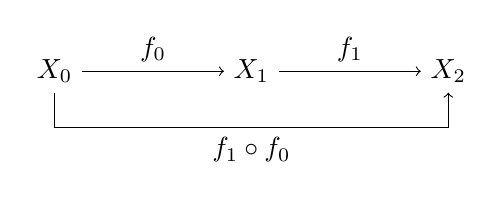
\begin{tikzpicture}[node distance=2.5cm, auto]
	\node (X) {$\bm{X_0}$};
	\node (Y) [right of=X] {$\bm{X_1}$};
	\node (n) [below of=Y,node distance=1cm] {$f_1 \circ f_0$};
	\node (Z) [right of=Y] {$\bm{X_2}$};
	\draw[->] (X) to node {$f_0$} (Y);
	\draw[->] (Y) to node {$f_1$} (Z);
%	\draw[->,bend right] (X) to node[swap] {$g \circ f$} (Z);
	\draw[->] (X) |- (n.90) -| (Z);\
\end{tikzpicture}
\end{figure}
	\end{enumerate}
\end{proposition}
\begin{proof}
\begin{enumerate}
	\item Seja $A \in \topo$. Então $\Id_X\inv(A)=A \in \topo$, logo $\Id_x$ é contínua.
	
	\item Seja $A \in \topo_2$. Como $f_1$ é contínua, $f_1\inv(A) \in \topo_1$. Como $f_0$ é contínua, $f_0\inv(f_1\inv(A)) \in \topo_0$. Portanto
		\begin{equation*}
		(f_1 \circ f_0)\inv(A) = f_1\inv \circ f_0\inv (A) = f_0\inv(f_1\inv(A)) \in \topo_0.
		\end{equation*}
	Logo $f_1 \circ f_0$ é contínua. \qedhere
\end{enumerate}
\end{proof}

\begin{definition}
Sejam $\bm{X_0}$ e $\bm{X_1}$ espaços topológicos. Um \emph{homeomorfismo} de $\bm{X_0}$ para $\bm{X_1}$ é uma função contínua $\fun{f}{\bm{X_0}}{\bm{X_1}}$ invertível cuja inversa é contínua. O conjunto de todos esses homeomorfismos é denotado por $\Iso{\Cont}(\bm{X_0},\bm{X_1})$.
Esses espaços topológicos são \emph{homeomorfos} e denota-se $\bm{X_0} \simeq \bm{X_1}$.
\end{definition}

\begin{exercise}
Sejam $\bm{X_0}$, $\bm{X_1}$ e $\bm{X_2}$ espaços topológicos.
		\begin{enumerate}
		\item (Reflexividade) $\bm{X_0} \simeq \bm{X_0}$;
		\item (Antissimetria) $\bm{X_0} \simeq \bm{X_1} \Rightarrow \bm{X_1} \simeq \bm{X_0}$;
		\item (Transitividade) $\bm{X_0} \simeq \bm{X_1} \text{\ \ e\ \ } \bm{X_1} \simeq \bm{X_2} \Rightarrow \bm{X_0} \simeq \bm{X_2}$.
		\end{enumerate}
\end{exercise}

\subsubsection{Suporte de funções vetoriais}

\begin{definition}
Sejam $\bm X$ um espaço topológico, $\bm L$ um espaço linear topológico e $f\colon X \to L$ uma função contínua. O \emph{suporte fechado} de $f$ é o conjunto
	\begin{equation*}
	\overline\supp(f) := \Fec{\supp(f)} = \Fec{f\inv(L \setminus \{0\})}.
	\end{equation*}
\end{definition}

\subsection{Topologias induzidas}

Nesta seção estudaremos como induzir topologias em conjuntos a partir de topologias que já temos. Isso será feito, em geral, de modo que uma ou mais funções sejam contínuas e a topologia induzida seja a menor ou a maior possível, dependendo do caso. Quando temos uma função de um conjunto em um espaço topológico, podemos induzir uma topologia nesse conjunto de modo que a topologia faça com  que a função seja contínua. Nesse caso, a maior topologia que faz a função ser contínua é a topologia discreta, e o nosso interesse será achar a menor topologia tal que a função é discreta. Quando temos uma função de um espaço topológico em um conjunto, o caso se inverte. A menor topologia tal que a função é contínua sempre é a topologia trivial, e o nosso interesse está na maior topologia que garante a continuidade. De maneira parecida, podemos induzir topologias garantindo a continuidade de várias funções e também considerando funções injetivas e sobrejetivas quado necessário. O estudo desta seção envolve a definição dessas noções e a investigação inicial como sobre esses objetos se comportam e por que são os menores ou maiores com determinadas características.

\subsubsection{Topologias puxada e inicial}

\begin{definition}
Sejam $X$ um conjunto, $\bm Y = (Y,\topo_Y)$ um espaço topológico e $f: X \to Y$ uma função. A \emph{topologia puxada} por $f$ de $\bm Y$ para $X$ é
	\begin{equation*}
	f^\star(\topo_Y) := \set{f^{-1}(A)}{A \in \topo_Y}.
	\end{equation*}
\end{definition}

\begin{proposition}
Sejam $X$ um conjunto, $\bm Y = (Y,\topo_Y)$ um espaço topológico e $f: X \to Y$ uma função. Então $f^\star(\topo_Y)$, a topologia puxada por $f$ de $\bm Y$ para $X$, é uma topologia de $X$.
\end{proposition}
\begin{proof}
(1) Notemos que, como $\emptyset \in \topo_Y$ e $\emptyset = f\inv(\emptyset)$, temos que $\emptyset \in f^\star(\topo_Y)$. (2) Seja $(A_i)_{i \in I}$ uma família de conjuntos em $f^\star(\topo_Y)$. Então, para cada $i \in I$, existe aberto $U_i \in \topo_Y$ tal que $A_i=f\inv(U_i)$. Como $\topo_Y$ é topologia, a união de abertos é aberto $\bigcup_{i \in I} U_i \in \topo_Y$. Portanto
	\begin{equation*}
	\bigcup_{i \in I} A_i = \bigcup_{i \in I} f\inv(U_i) = f\inv\left( \bigcup_{i \in I} U_i\right),
	\end{equation*}
logo $\bigcup_{i \in I} A_i \in f^\star(\topo_Y)$.
(3) Seja $(A_i)_{i=1}^n$ uma família de conjuntos em $f^\star(\topo_Y)$. Então, para cada $1 \leq i \leq n$, existe aberto $U_i \in \topo_Y$ tal que $A_i=f\inv(U_i)$. Como $\topo_Y$ é topologia, a interseção finita de abertos é aberto $\bigcap_{i=1}^n U_i \in \topo_Y$. Portanto
	\begin{equation*}
	\bigcap_{i=1}^n A_i = \bigcap_{i=1}^n f\inv(U_i) = f\inv\left( \bigcap_{i=1}^n U_i\right),
	\end{equation*}
logo $\bigcap_{i=1}^n A_i \in f^\star(\topo_Y)$.
\end{proof}

\begin{proposition}
\label{topo:prop.cont.topo.pux}
Sejam $\bm X = (X,\topo_ X)$ e $\bm Y = (Y,\topo_ Y)$ espaços topológicos. Uma função $f: X \to Y$ é função contínua de $\bm X$ para $\bm Y$ se, e somente se, a topologia $f^\star(\topo_Y)$ puxada por $f$ de $\bm Y$ para $X$ é uma subtopologia de $\topo_ X$.
	\begin{equation*}
	f \in \Cont(\bm X,\bm Y) \sse f^\star(\topo_Y) \subseteq \topo_X.
	\end{equation*}
\end{proposition}
\begin{proof}
Suponha que $f \in \Cont(\bm X,\bm Y)$ e seja $B \in f^\star(\topo_Y)$. Então existe $A \in \topo_Y$ tal que $B=f\inv(A)$. Como $f$ é contínua, segue que $f\inv(A) \in \topo_X$, portanto, $f^\star(\topo_Y) \subseteq \topo_X$. Reciprocamente, suponha que $f^\star(\topo_Y) \subseteq \topo_X$. Então, para todo $A \in \topo_Y$, $f\inv(A) \in f^\star(\topo_Y)$, portanto $f\inv(A) \in \topo_X$, o que mostra que $f \in \Cont(\bm X,\bm Y)$.
\end{proof}

\begin{definition}
Sejam $\bm X$ um conjunto, $(\bm{X_i})_{i \in I} = (X_i,\topo_i)_{i \in I}$ uma família de espaços topológicos e, para todo $i \in I$, $f_i: X \to X_i$ uma função. A \emph{topologia inicial} de $X$ com respeito à família $(f_i)_{i \in I}$ é a menor topologia de $X$ tal que, para todo $i \in I$, $f_i$ é contínua.
\end{definition}

\begin{proposition}
Sejam $\bm X$ um conjunto, $(\bm{X_i})_{i \in I} = (X_i,\topo_i)_{i \in I}$ uma família de espaços topológicos e, para todo $i \in I$, $f_i: X \to X_i$ uma função. A topologia inicial de $X$ com respeito à família $(f_i)_{i \in I}$ é a topologia
	\begin{equation*}
	\ger{\bigcup_{i \in I} {f_i}^\star(\topo_i)}.
	\end{equation*}
\end{proposition}
\begin{proof}
Seja $\topo$ uma topologia de $X$ tal que, para todo $i \in I$, $f_i: X \to X_i$ é contínua. Então, para todo $i \in I$, ${f_i}^\star(\topo_i) \subseteq \topo$ (\ref{topo:prop.cont.topo.pux}), o que implica que $\bigcup_{i \in I} {f_i}^\star(\topo_i) \subseteq \topo$ e, portanto, $\ger{\bigcup_{i \in I} {f_i}^\star(\topo_i)} \subseteq \topo$.
\end{proof}

\subsubsection{Topologias empurrada e final}

\begin{definition}
Sejam $\bm X = (X,\topo_X)$ um espaço topológico, $Y$ um conjunto e $f: X \to Y$ uma função. A \emph{topologia empurrada} por $f$ de $\bm X$ para $Y$ é
	\begin{equation*}
	f_\star(\topo_X) := \set{A \subseteq Y}{f^{-1}(A) \in \topo_X}.
	\end{equation*}
\end{definition}

\begin{proposition}
Sejam $\bm X = (X,\topo_X)$ um espaço topológico, $Y$ um conjunto e $f: X \to Y$ uma função. Então $\topo_Y := f_\star(\topo_X)$, a topologia empurrada por $f$ de $\bm X$ para $Y$, é uma topologia de $Y$.
\end{proposition}
\begin{proof}
(1) Como $f\inv(\emptyset)=\emptyset$ e $f\inv(Y)=X$, segue que $\emptyset,Y \in f_\star(\topo_X)$. (2) Seja $(A_i)_{i \in I}$ uma família de conjuntos de $f_\star(\topo_X)$. Então, para cada $i \in I$, $f\inv(A_i) \in \topo_X$, o que implica que
\begin{equation*}
	f\inv \left( \bigcup_{i \in I} A_i \right) = \bigcup_{i \in I} f\inv(A_i) \in \topo_X,
	\end{equation*}
portanto $\bigcup_{i \in I} A_i \in f_\star(\topo_X)$. (3) Seja $(A_i)_{i=1}^n$ uma família de conjuntos de $f_\star(\topo_X)$. Então, para cada $1 \leq i \leq n$, $f\inv(A_i) \in \topo_X$, o que implica que
\begin{equation*}
	f\inv \left( \bigcap_{i=1}^n A_i \right) = \bigcap_{i=1}^n f\inv(A_i) \in \topo_X,
	\end{equation*}
portanto $\bigcap_{i=1}^n A_i \in f_\star(\topo_X)$.
\end{proof}

\begin{definition}
Sejam $\bm X$ um conjunto, $(\bm{X_i})_{i \in I} = (X_i,\topo_i)_{i \in I}$ uma família de espaços topológicos e, para todo $i \in I$, $f_i: X_i \to X$ uma função. A \emph{topologia final} de $X$ com respeito à família $(f_i)_{i \in I}$ é a maior topologia de $X$ tal que, para todo $i \in I$, $f_i$ é contínua.
\end{definition}

\begin{proposition}
Sejam $\bm X$ um conjunto, $(\bm{X_i})_{i \in I} = (X_i,\topo_i)_{i \in I}$ uma família de espaços topológicos e, para todo $i \in I$, $f_i: X_i \to X$ uma função. A topologia final de $X$ com respeito à família $(f_i)_{i \in I}$ é a topologia
	\begin{equation*}
	\bigcap_{i \in I} {f_i}_\star(\topo_i).
	\end{equation*}
\end{proposition}
\begin{proof}
Seja $\topo$ uma topologia de $X$ tal que, para todo $i \in I$, $f_i: X_i \to X$ é contínua, e seja $A \in \topo$. Então, para todo $i \in I$, $f_i \inv(A) \in \topo_i$, o que implica que $A \in {f_i}_\star(\topo_i)$, portanto $A \in \bigcap_{i \in I} {f_i}_\star(\topo_i)$. Isso mostra que $\topo \subseteq \bigcap_{i \in I} {f_i}_\star(\topo_i)$, e como interseção de topologias é topologia, segue o procurado.
\end{proof}

\subsubsection{Produto de espaços topológicos}

\begin{definition}
Seja $(\bm{X_i})_{i \in I} = (X_i,\topo_i)_{i \in I}$ uma família de espaços topológicos. O \emph{produto} da família $(\bm{X_i})_{i \in I}$ é o par
	\begin{equation*}
	\prod_{i \in I} \bm{X_i} := \left( \prod_{i \in I} X_i , \ger{\bigcup_{i \in I}{\pi_i}^\star(\topo_i)} \right).
	\end{equation*}
A topologia $\ger{\bigcup_{i \in I}{\pi_i}^\star(\topo_i)}$ é a \emph{topologia produto} de $\prod_{i \in I} X_i$.
\end{definition}

\begin{proposition}
Sejam $(\bm{X_i})_{i \in I} = (X_i,\topo_i)_{i \in I}$ uma família de espaços topológicos e $X = \prod_{i \in I} X_i$ o produto de conjuntos. A topologia produto de $X$ é a topologia gerada pela base cujos elementos são $\prod_{i \in I} A_i$, tal que $A_i \in \topo_i$ e existe $J \subseteq I$ finito com $A_i = X_i$ para $i \in I \setminus J$.
\end{proposition}
\begin{proof}
Como $\pi_i = \pi_i \circ \Id_X$, segue de uma propriedades básica de imagem inversa de produto (\ref{conj:prop.im.inv.prod}) que
	\begin{equation*}
	\prod_{i \in I} A_i = \Id_X\inv \left(\prod_{i \in I} A_i\right) = \bigcap_{i \in I} \pi_i\inv(A_i)
	\end{equation*}
Para todo $i \in I \setminus J$, $A_i=X_i$, então $\pi_i\inv(A_i)=X$ e, portanto,
	\begin{equation*}
	\bigcap_{i \in I\setminus J} \pi_i\inv(A_i) = \bigcap_{i \in I\setminus J} X = X.
	\end{equation*}
Isso implica que
	\begin{equation*}
	\bigcap_{i \in I} \pi_i\inv(A_i) = \left(\bigcap_{i \in I\setminus J} \pi_i\inv(A_i)\right) \cap \left(\bigcap_{j \in J} \pi_j\inv(A_j)\right) =  \bigcap_{j \in J} \pi_j\inv(A_j)
	\end{equation*}
Logo $\prod_{i \in I} A_i = \bigcap_{j \in J} \pi_j\inv(A_j)$. Seja $A$ aberto da topologia descrita na proposição. Então
	\begin{equation*}
	A = \bigcup_{k \in K} A_k = \bigcup_{k \in K}\prod_{i \in I} A_{ki} = \bigcup_{k \in K}\bigcap_{j \in J} \pi_j\inv (A_{kj}),
	\end{equation*}
o que mostra que $A$ é aberto da topologia produto. O resto da demonstração é simples.
\end{proof}

\begin{proposition}[Propriedade Universal]
Sejam $(\bm{X_i})_{i \in I} = (X_i,\topo_i)_{i \in I}$ uma família de espaços topológicos, $\bm T = (T,\topo_T)$ um espaço topológico e, para todo $i \in I$, $f_i: \bm T \to \bm{X_i}$ uma função contínua. Então existe uma única função contínua $f: \bm T \to \prod_{i \in I} \bm{X_i}$ tal que, para todo $i \in I$, $\pi_i \circ f = f_i$ (o diagrama comuta).
\begin{figure}
\centering
\begin{tikzpicture}[node distance=2.5cm, auto]
	\node (P) {$\displaystyle\prod_{i \in I} \bm{X_i}$};
	\node (Ci) [below of=P] {$\bm{X_i}$};
	\node (X) [left of=Ci] {$\bm{T}$};
	\draw[->] (X) to node [swap] {$f_i$} (Ci);
	\draw[->, dashed] (X) to node {$f$} (P);
	\draw[->] (P) to node {$\pi_i$} (Ci);
\end{tikzpicture}
\end{figure}
\end{proposition}
\begin{proof}
Defina a função
	\begin{align*}
	\func{f}{T}{ \prod_{i \in I} X_i}{ x}{ (f_i(x))_{i \in I}}.
	\end{align*}
Pela propriedade universal do produto de conjuntos, $f$ é única e $\pi_i \circ f = f_i$. Resta mostrar que $f$ é contínua. Seja $A \in \topo_X$. Então $A=\bigcup_{k \in K} A_k$ é uma união de abertos básicos $A_k \in \topo$. Isso significa que, para todo $k \in K$, $A_k = \prod_{i \in I} A_{ki}$, com $A_{ki} \in \topo_i$ para todo $i \in I$ e existe $J_k \subseteq I$ finito tal que, para todo $i \in I \setminus J_k$, $A_{ki} = X_i$. Assim, por propriedades básicas de imagem inversa de união e produto (\ref{conj:prop.im.inv.prod}),
		\begin{equation*}
		f\inv(A) = f\inv\left(\bigcup_{k \in K}\prod_{i \in I} A_{ki}\right) = \bigcup_{k \in K} f\inv \left( \prod_{i \in I} A_{ki} \right) = \bigcup_{k \in K}\bigcap_{i \in I}f_i\inv(A_{ki}).
		\end{equation*}
Seja $k \in K$. Como, para todo $i \in I \setminus J_k$, $A_{ki} = X_i$, então $f_i\inv(A_{ki}) = f_i\inv(X_i) = T$. Disso segue que
	\begin{equation*}
	\bigcap_{i \in I}f_i\inv(A_{ki}) = \bigcap_{j \in J_k}f_j\inv(A_{kj})
	\end{equation*}
e, portanto,
	\begin{equation*}
	f\inv(A) = \bigcup_{k \in K}\bigcap_{j \in J_k}f_j\inv(A_{kj}).
	\end{equation*}
Seja $k \in K$. Para todo $j \in J_k$, $f_j$ é contínua, o que implica que $f_j\inv(A_{kj})$ é aberto e, por $J_k$ ser finito, a interseção $\bigcap_{j \in J_k}f_j\inv(A_{kj})$ é aberta. Isso significa que a união $\bigcup_{k \in K}\bigcap_{j \in J_k}f_j\inv(A_{kj})$ é aberta e, portanto, $f\inv(A) \in \topo_T$. Logo $f$ é contínua.
\end{proof}

\subsubsection{Coproduto de espaços topológicos}

\begin{definition}
Seja $(\bm{X_i})_{i \in I} = (X_i,\topo_i)_{i \in I}$ uma família de espaços topológicos. O \emph{coproduto} da família $(\bm{X_i})_{i \in I}$ é o par
	\begin{equation*}
	\coprod_{i \in I} \bm{X_i} := \left( \coprod_{i \in I} X_i , \bigcap_{i \in I}{\iota_i}_\star(\topo_i) \right).
	\end{equation*}
A topologia $\bigcap_{i \in I}{\pi_i}_\star(\topo_i)$ é a \emph{topologia coproduto} de $\coprod_{i \in I} X_i$.
\end{definition}

\begin{proposition}[Propriedade Universal]
Sejam $(\bm{X_i})_{i \in I} = (X_i,\topo_i)_{i \in I}$ uma família de espaços topológicos, $\bm T = (T,\topo_T)$ um espaço topológico e, para todo $i \in I$, $f_i: \bm{X_i} \to \bm T$ uma função contínua. Então existe uma única função contínua $f: \coprod_{i \in I} \bm{X_i} \to \bm T$ tal que, para todo $i \in I$, $f \circ \iota_i = f_i$ (o diagrama comuta).
\begin{figure}
\centering
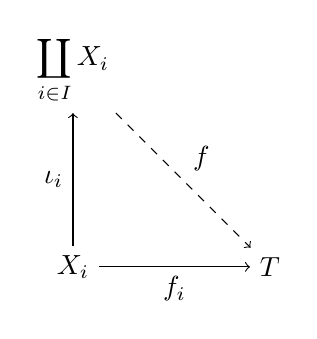
\begin{tikzpicture}[node distance=2.5cm, auto]
	\node (Ci) {$\bm{X_i}$};
	\node (S) [above of=Ci] {$\displaystyle\coprod_{i \in I} \bm{X_i}$};
	\node (X) [right of=Ci] {$\bm T$};
	\draw[->] (Ci) to node [swap] {$f_i$} (X);
	\draw[->, dashed] (S) to node {$f$} (X);
	\draw[->] (Ci) to node {$\iota_i$} (S);
\end{tikzpicture}
\end{figure}
\end{proposition}

\subsubsection{Subespaços topológicos}

\begin{definition}
Sejam $(X,\topo)$ um espaço topológico e $S \subseteq X$ um subconjunto. A \emph{topologia induzida} por $\topo$ em $S$ é o conjunto
	\begin{equation*}
	\topo|_S := \set{A \cap S}{A \in \topo}.
	\end{equation*}
\end{definition}

\begin{proposition}
Sejam $(X,\topo)$ um espaço topológico e $S \subseteq X$ um subconjunto. A topologia induzida por $\topo$ em $S$ é o conjunto
	\begin{equation*}
	\topo|_S = \iota_\star(\topo),
	\end{equation*}
a maior topologia tal que a inclusão $\iota: S \to X$ é contínua.
\end{proposition}

\begin{proposition}
Sejam $(X,\topo)$ um espaço topológico e $S \subseteq X$ um subconjunto. A topologia induzida por $\topo$ em $S$ é uma topologia de $S$.
\end{proposition}
\begin{proof}
(1) Notemos que $\emptyset,S \in \topo|_S$, pois $\emptyset \cap S = \emptyset$ e $X \cap S = S$. (2) Seja $(A_i)_{i \in I}$ uma família de abertos de $\topo|_S$. Então, para cada $i \in I$, existe um aberto $B_i \in \topo$ tal que $A_i = B_i \cap S$. Assim, temos que
	\begin{equation*}
	\bigcup_{i \in I} A_i = \bigcup_{i \in I} (B_i \cap S) = \left( \bigcup_{i \in I} B_i \right) \cap S,
	\end{equation*}
que pertence à topologia induzida pois $\bigcup_{i \in I} B_i \in \topo$. (3) Seja $(A_i)_{i=1}^n$ uma família de abertos de $\topo|_S$. Então, para cada $1 leq i leq n$, existe um aberto $B_i \in \topo$ tal que $A_i = B_i \cap S$. Assim, temos que
	\begin{equation*}
	\bigcap_{i=1}^n A_i = \bigcap_{i=1}^n (B_i \cap S) = \left( \bigcap_{i=1}^n B_i \right) \cap S,
	\end{equation*}
que pertence à topologia induzida pois $\bigcap_{i=1}^n B_i \in \topo$.
\end{proof}

\begin{proposition}[Propriedade característica]
Sejam $\bm X=(X,\topo_X)$ e $(Y,\topo_Y)$ espaços topológicos e $\bm S \subseteq \bm X$ um subespaço. Uma função $f\colon Y \to S$ é contínua se, e somente se, $\iota \circ f: Y \to X$ é contínua (o diagrama comuta).
\begin{figure}
\centering
\begin{tikzpicture}[node distance=2.5cm, auto]
	\node (X) {$\bm X$};
	\node (S) [below of=X] {$\bm S$};
	\node (Y) [left of=S] {$\bm{T}$};
	\draw[->] (Y) to node [swap] {$f$} (S);
	\draw[->] (Y) to node {$\iota \circ f$} (X);
	\draw[->] (S) to node [swap] {$\iota$} (X);
\end{tikzpicture}
\end{figure}
\end{proposition}

\paragraph*{Proposição} Restrição de função contínua é contínua na topologia induzida.

\begin{proposition}[Colagem por abertos]
Sejam $\bm X$ e $\bm Y$ espaços topológicos, $f: X \to Y$ uma função e $(X_i)_{i \in I}$ uma cobertura de $X$ por conjuntos abertos tal que, para todo $i \in I$, $f|_{X_i}: X_i \to Y$ é contínua. Então $f: X \to Y$ é contínua.
\end{proposition}

\begin{proposition}[Colagem por fechados]
Sejam $\bm X$ e $\bm Y$ espaços topológicos, $f: X \to Y$ uma função e $(X_i)_{i=1}^n$ uma cobertura de $X$ por conjuntos fechados tal que, para todo $1 \leq i \leq n$, $f|_{X_i}: X_i \to Y$ é contínua. Então $f: X \to Y$ é contínua.
\end{proposition}

\subsubsection{Quociente de espaços topológicos}

\begin{definition}
Sejam $\bm X = (X,\topo)$ um espaço topológico e $\sim$ uma relação de equivalência em $X$. O \emph{espaço quociente} com respeito a $\sim$ é o espaço topológico
	\begin{equation*}
	\bm{\quo{X}{\sim}} := \left( \quo{X}{\sim}, \pi^\star(\topo) \right),
	\end{equation*}
em que $\pi: X \to \quo{X}{\sim}$ é a projeção canônica de equivalências.
\end{definition}

É fácil notar que os abertos de $\bm{\quo{X}{\sim}}$ são conjuntos de classes de equivalência cuja união é um aberto de $\bm X$. Notemos, ainda, que se $f: X \to Y$ é sobrejetivo, existe uma relação de equivalência em $X$ induzida por $f$, definida como dois elementos são equivalentes se suas imagens são iguais, e essa relação de equivalência faz com que possamos identificar $Y$ com $\quo{X}{\sim}$ como conjuntos. Definimos a topologia em $Y$ de modo que $Y$ e $\quo{X}{\sim}$ sejam homeomorfos.

\begin{proposition}[Propriedade característica]
Sejam $\bm X=(X,\topo_X)$ e $(Y,\topo_Y)$ espaços topológicos e $\bm Q$ um espaço quociente de $\bm X$. Uma função $f: Q \to Y$ é contínua se, e somente se, $f \circ \pi: X \to Y$ é contínua (o diagrama comuta).
\begin{figure}
\centering
\begin{tikzpicture}[node distance=2.5cm, auto]
	\node (Q) {$\bm Q$};
	\node (X) [above of=Q] {$\bm X$};
	\node (Y) [right of=Q] {$\bm Y$};
	\draw[->] (Q) to node [swap] {$f$} (Y);
	\draw[->] (X) to node {$f \circ \pi$} (Y);
	\draw[->] (X) to node [swap] {$\pi$} (Q);
\end{tikzpicture}
\end{figure}
\end{proposition}

\paragraph{Soma pontual}

\begin{definition}
Sejam $(\bm X_0,x_0)$ e $(\bm X_1,x_1)$ espaços topológicos pontuados. A \emph{soma pontual} de $\bm X_0$ e $\bm X_1$ é o espaço quociente
	\begin{equation*}
	\bm X_0 \dotplus \bm X_1 := \quo{\bm X_0 \sqcup \bm X_1}{\sim},
	\end{equation*}
em que $\sim$ é a menor equivalência tal que $(0,x_0) \sim (1,x_1)$.
\end{definition}

\begin{definition}
Sejam $(\bm X_i,x_i)_{i \in I}$ espaços topológicos pontuados. A \emph{soma pontual} de $(\bm X_i,x_i)_{i \in I}$ é o espaço quociente
	\begin{equation*}
	\bigdotplus_{i \in I} X_i := \quo{\bigsqcup X_i}{\sim},
	\end{equation*}
em que $\sim$ é a menor equivalência tal que, para todos $i,i' \in I$, $(i,x_i) \sim (i',x_{i'})$.
\end{definition}

\paragraph{Exemplo de topologia quociente para soma pontual de esferas}

Consideremos uma esfera $d$-dimensional $\S^d$ e o espaço $\S^s \dotplus \S^d$, dado aqui por
	\begin{align*}
	\S^d \dotplus \S^d &= (\frac{1}{2}\S^d + (\frac{1}{2},0,\ldots,0)) \cup (\frac{1}{2}\S^d - (\frac{1}{2},0,\ldots,0)) \\
		&= \set{x \in \R^{d+1}}{\nor{x-(\frac{1}{2},0,\ldots,0)}=\frac{1}{2}} \cup \set{x \in \R^{d+1}}{\nor{x+(\frac{1}{2},0,\ldots,0)}=\frac{1}{2}}.
	\end{align*}

Definimos assim a função
	\begin{align*}
	\func{\mathrm{q}}{\S^d}{\S^d \dotplus \S^d}{(x_0,\ldots,x_d)}{\left( x_0, \left( \frac{\abs{x_0}-{x_0}^2}{1-{x_0}^2} \right)^{\frac{1}{2}} x_1, \ldots, \left( \frac{\abs{x_0}-{x_0}^2}{1-{x_0}^2} \right)^{\frac{1}{2}} x_d \right)}
	\end{align*}

Essa função é uma função quociente. Primeiro, mostremos que ela está bem definida. Seja $x \in \S^d$.

\subsection{Topologia de ordem}

Lembremos que, se $(X,\leq)$ é um conjunto (totalmente) ordenado e $e,e' \in X$, o intervalo aberto de extremos inferior $e$ e superior $e'$ é o conjunto
	\begin{equation*}
	\intaa{e}{e'}= \set{x \in X}{e < x < e'}.
	\end{equation*}
As semirretas abertas são os intervalos
	\begin{equation*}
	\intaa{e}{\infty} := \set{x \in X}{e < x}
	\end{equation*}
e
	\begin{equation*}
	\intaa{-\infty}{e} := \set{x \in X}{x < e}.
	\end{equation*}

%Definindo a função $m_e(x) = \min\{x,e\}$. Então
%	\begin{equation*}
%	\intaa{-\infty}{e} = {m_e}\inv(X).
%	\end{equation*}

\begin{definition}
Seja $(X,\leq)$ um conjunto ordenado. A \emph{topologia de ordem} sobre $X$ é a topologia gerada pelas semirretas abertas de $(X,\leq)$. %pelos intervalos abertos $\intaa{e}{e'}$.
Denotamos essa topologia por $\topo_\leq$ (ou simplesmente $\topo$ se for claro pelo contexto).
\end{definition}

\begin{proposition}
Seja $(X,\leq)$ um conjunto ordenado. O par $(X,\topo_\leq)$ é um espaço topológico hereditariamente normal com base de intervalos abertos.
\end{proposition}

\subsubsection{Topologia de um corpo ordenado}

Lembremos que, se $(X,\leq)$ é um espaço ordenado, a topologia $\topo_\leq$ induzida por $\leq$ é a topologia gerada pelas semirretas abertas $\intaa{x}{\infty}$ e $\intaa{\infty}{x}$, e o conjunto de intervalos abertos $\intaa{x}{x'}$ é uma base de $\topo_\leq$.

Note que
	\begin{align*}
	\bigcup_{i \in I} \intaa{e_i}{e'_i} &= \intaa{\inf_{i \in I} e_i}{\sup_{i \in I} e'_i} \\
	\bigcap_{i \in I} \intff{e_i}{e'_i} &= \intff{\sup_{i \in I} e_i}{\inf_{i \in I} e'_i}.
	\end{align*}

\begin{proposition}
Seja $(\bm C,\leq)$ um corpo ordenado. O par $(\bm C,\topo_\leq)$ é um corpo topológico.
\end{proposition}
\begin{proof}
Precisamos mostrar que $+$, $-$, $\times$ e $\inv$ são contínuas. Para isso, basta mostrar que elas puxam abertos geradores para abertos. Seja $e \in C$ e consideremos as semirretas $\intaa{e}{\infty}$ e $\intaa{-\infty}{e}$. Para mostrar que $+$ é contínua, notamos que, se $c+c' > e$, então $c' > e-c$, logo
	\begin{equation*}
	+\inv \big( \intaa{e}{\infty} \big) = \bigcup_{c \in C} \big( \intaa{c}{\infty} \times \intaa{e-c}{\infty} \big)
	\end{equation*}
e, analogamente,
	\begin{equation*}
	+\inv \big( \intaa{-\infty}{e} \big) = \bigcup_{c \in C} \big( \intaa{-\infty}{c} \times \intaa{-\infty}{e-c} \big),
	\end{equation*}
que são abertos pois são uniões de abertos, o que implica que $+$ é contínua. Para mostrar que $-$ é contínua, notamos que
	\begin{equation*}
	-\inv \big( \intaa{e}{\infty} \big) = \intaa{-\infty}{-e}
	\end{equation*}
e
	\begin{equation*}
	-\inv( \intaa{-\infty}{e} ) = \intaa{-e}{\infty},
	\end{equation*}
que são ambos abertos, o que mostra que $-$ é contínua.

Para mostrar que $\times$ é contínua, consideramos dois casos. 

(1) Se $e=0$ e $c \times c' > e=0$, então $c \neq 0$, logo se $c > 0$ então $c'>0$ e, se $c < 0$, então $c' < 0$, logo
	\begin{equation*}
	\times\inv \big( \intaa{0}{\infty} \big) = \big( \intaa{0}{\infty} \times \intaa{0}{\infty} \big) \cup \big( \intaa{-\infty}{0} \times \intaa{-\infty}{0} \big)
	\end{equation*}
e, analogamente,
	\begin{equation*}
	\times\inv \big( \intaa{-\infty}{0} \big) = \big( \intaa{0}{\infty} \times \intaa{-\infty}{0} \big) \cup \big( \intaa{-\infty}{0} \times \intaa{0}{\infty} \big),
	\end{equation*}
que são ambos abertos;
%	\begin{equation*}
%	\times\inv ( \intaa{0}{\infty} ) = \bigcup_{c \in C_{>0}} \big( \intaa{c}{\infty} \times \intaa{0}{\infty} \big) \cup \bigcup_{c \in C_{<0}} \big( \intaa{\infty}{c} \times \intaa{-\infty}{0} \big)
%	\end{equation*
%(2) se $e > 0$ e $c \times c' > e > 0$, então $c \neq 0$,
%
%notamos que, se $c \times c' > e$, existem dois casos: (1) se $e=0$, então $c \neq 0$, logo $c' > c$
%
%
%(1) se $c \neq 0$, então $c' \geq e/c$; se $c=0$, então e caso contr
%
%
%	\begin{equation*}
%	\times\inv ( \intaa{e}{\infty} ) = \bigcup_{c \in C \setminus \{0\}} \intaa{c}{\infty} \times \intaa{e/c}{\infty}
%	\end{equation*}
%pois
o caso (2) em que $e \neq 0$ é análogo, embora um pouco mais trabalhoso. Isso mostra que $\times$ é contínua. Mostrar que $\inv$ é contínua também é trabalhoso, mas segue direto de modo análogo.
%Para mostrar que $/$ é contínua, notamos que
%	\begin{equation*}
%	{/}\inv \big( \intaa{0}{\infty} \big)
%	\end{equation*}
\end{proof}



% Topologicamente falando, qual a consequência de um corpo ser infinitesimal/arquimediano?




\begin{proposition}
Seja $(\bm C,\leq)$ um corpo ordenado. O corpo topológico $(\bm C,\topo_\leq)$ é separado.
\end{proposition}
\begin{proof}
Sejam $c,c' \in C$ tais que $c \neq c'$. Então $c < c'$ ou $c' < c$. Sem perda de generalidade, considere que $c < c'$. Então as vizinhanças
	\begin{equation*}
	\intaa{-\infty}{\frac{c+c'}{2}} \qquad\text{e}\qquad \intaa{\frac{c+c'}{2}}{\infty}
	\end{equation*}
de $c$ e $c'$, respectivamente, separam $c$ e $c'$.
\end{proof}

% MOSTRAR QUE É NORMAL
%Qualquer aberto é da forma
%	\begin{equation*}
%	\bigcup_{i \in I} \intaa{e_i}{e'_i},
%	\end{equation*}
%em que $e_i < e'_i$, mas $e_i,e'_i$ podem ser, respectivamente, $-\infty$ e $\infty$. Isso implica que qualquer fechado é da forma
%	\begin{align*}
%	F = \left( \bigcup_{i \in I} \intaa{e_i}{e'_i} \right)^\complement &= \bigcap_{i \in I} \big( \intaa{e_i}{e'_i} \big)^\complement \\
%		&= \bigcap_{i \in I} \big( \intaa{-\infty}{e_i} \cup \intaa{e'_i}{\infty} \big) \\
%%		&= \left( \bigcap_{i \in I} \intaa{-\infty}{e_i} \right) \cup \left( \bigcap_{i \in I}\intaa{e'_i}{\infty} \right) \\
%%		&= 
%	\end{align*}
%
%Agora, seja $c \notin F$. Então $c \in \bigcup_{i \in I} \intaa{e_i}{e'_i}$, o que significa que existe algum $i \in I$ tal que $c \in \intaa{e_i}{e'_i}$.

% Tem no stack exchange como mostrar que todo espaço métrico é completamente normal, deve dar pra estender pra espaços "métricos" com uma distância a valores no cone positivo de um corpo ordenado.

Consideremos em $C_{\geq 0}$ a topologia induzida.

\begin{proposition}
Seja $(\bm C,\leq)$ um corpo ordenado. As funções valor absoluto $\abs{\var}\colon C \to C_{\geq 0}$ e distância $\dist{\var}{\var}\colon C \times C \to C_{\geq 0}$ são contínuas.
\end{proposition}
\begin{proof}
(Valor absoluto) Seja $c \in C_{\geq 0}$ e consideremos os abertos $\intaa{c}{\infty}$ e $\intfa{0}{c}$. Então
	\begin{equation*}
	\abs{\var}\inv \big( \intaa{c}{\infty} \big) = \intaa{-\infty}{-c} \cup \intaa{c}{\infty}
	\end{equation*}
e
	\begin{equation*}
	\abs{\var}\inv \big( \intfa{0}{c} \big) = \intaf{-c}{0} \cup \intfa{0}{c} = \intaa{-c}{c},
	\end{equation*}
que são ambos abertos, o que mostra que $\abs{\var}$ é contínua.

(Distância) Como $\dist{\var}{\var}$ é composição de $\abs{\var}$, $+$, $-$, $\proj_0$ e $\proj_1$, que são todas contínuas, segue que ela é contínua.
%	\begin{equation*}
%	\dist{c}{c'} := \abs{c'-c}
%	\end{equation*}
%	\begin{align*}
%	\dist{\var}{\var} &= \dist{\var}{\var} \circ \Id \\
%		&= \dist{\var}{\var} \circ (\proj_0,\proj_1) \\
%		&= \dist{\proj_0}{\proj_1} \\
%		&= \abs{\proj_1-\proj_0} \\
%		&= \abs{\var} \circ (+(\proj_1,- \circ \proj_0)).
%	\end{align*}
\end{proof}





\begin{proposition}
Seja $(\bm C,\leq)$ um corpo ordenado. O corpo $\bm C$ é não-infinitesimal se, e somente se, $\Q_C$ é denso em $C$.
\end{proposition}

\section{Separação}

\subsection{Noções de separação de conjuntos}

Nesta seção são apresentadas algumas noções de como dois conjuntos de um espaço topológico podem ser separados. As duas noções mas simples de separação são noções conjuntistas. A primeira é a de conjuntos distintos, ou diferentes, $A \neq B$, e a outra é a de conjuntos disjuntos, $A \cap B = \emptyset$. A seguir, mostramos noções que envolvem construções topológicas e não meramente conjuntistas.

\begin{definition}
Sejam $\bm X$ um espaço topológico e $A,B \subseteq X$. Definimos as seguintes relações entre $A$ e $B$:
	\begin{enumerate}
	\item (\emph{Separação}) Cada conjunto é disjunto do fecho do outro.
	\begin{equation*}
	A \cap \Fec{B} = \Fec{A} \cap B = \emptyset.
	\end{equation*}
	\item (\emph{Separação por vizinhanças}) Existem vizinhanças $V_A \in \viz_A$ e $V_B \in \viz_B$ que são disjuntas.
	\begin{equation*}
	V_A \cap V_B = \emptyset.
	\end{equation*}
	\item (\emph{Separação por função contínua}) Existe uma função contínua $f \in \Cont(X,[0,1])$ tal que
	\begin{equation*}
	f(A)=\{0\} \text{\ \ e\ \ } f(B)=\{1\}.
	\end{equation*}
	\item (\emph{Separação precisa por função contínua}) Existe uma função contínua $f \in \Cont(X,[0,1])$ tal que
	\begin{equation*}
	f\inv(\{0\})=A \text{\ \ e\ \ } f\inv(\{1\})=B.
	\end{equation*}
	\end{enumerate}
Cada uma das relações vale entre pontos $x,y \in X$, ou entre um conjunto $A$ e um ponto $x$, ao considerarmos no lugar no ponto o conjunto unitário que o contém: valem entre os conjuntos $\{x\}$ e $\{y\}$, ou entre $A$ e $\{x\}$, respectivamente.
\end{definition}

	As primeiras duas relações binárias são claramente simétricas, mas isso não é necessariamente claro no caso da terceira e quarta. No entanto, isso pode ser concluído ao considerar, dada uma função $f$ que faz $A$ e $B$ separados por função contínua, a função $1-f$ que faz o mesmo entre $B$ e $A$.

\begin{proposition}
\label{topo:prop.separacao}
Sejam $\bm X$ um espaço topológico e $A,B \subseteq X$. Então
	\begin{enumerate}
	\item Se $A$ e $B$ são precisamente separados por função contínua, então são separados por função contínua.
	\item Se $A$ e $B$ são separados por função contínua, então são separados por vizinhanças.
	\item Se $A$ e $B$ são separados por vizinhanças, então são separados.
	\item Se $A$ e $B$ são separados, então são disjuntos.
	\end{enumerate}
\end{proposition}
%\begin{proof}
%Suponhamos que existe função contínua $f:X \to [0,1]$ tal que $f(A)= \{0\}$ e $f(B)=\{1\}$. Definamos $U := f^{-1}(\left[0,\frac{1}{2}\right))$ e $V := f^{-1}((\frac{1}{2},1))$. Como $f$ é contínua, $U$ e $V$ são abertos. Ainda, $A \subseteq U$ e $B \subseteq V$. Por fim, como $U \cap V = \emptyset$, concluímos que $\bm X$ é normal.
%\end{proof}

% DÚVIDA: As relações de separação negadas são relações de equivalência? Pois indintinguibilidade topológica é, e ela é a negação de separação de pontos (não exatamente). Tentar entender melhor isso.


\subsection{Espaços distinguíveis}

\begin{definition}
Seja $\bm X$ um espaço topológico. Pontos \emph{topologicamente indistinguíveis} em $\bm X$ são pontos $x,y \in X$ tais que $\viz_x = \viz_y$. Pontos \emph{topologicamente disntinguíveis em $\bm X$} são pontos que não são topologicamente indistinguíveis.
\end{definition}

\begin{proposition}
Seja $\bm X$ um espaço topológico. A relação binária de indistinguibilidade topológica é uma relação de equivalência em $X$.
\end{proposition}
\begin{proof}
Denotemos por $\sim$ a relação binária de indistinguibilidade topológica. Sejam $x,y,z \in X$. Para mostrar a reflexividade, notemos que, como $\viz_x=\viz_y$, então $x \sim x$. Para mostrar a simetria, se $x \sim y$, então $\viz_x=\viz_y$, o que é equivalente a $\viz_y=\viz_x$ e, portanto, $y \sim x$. Por fim, para mostrar a transitividade, se $x \sim y$ e $y \sim z$, então $\viz_x=\viz_y$ e $\viz_y=\viz_z$, o que implica $\viz_x=\viz_z$ e, portanto, $x \sim z$.
\end{proof}

O fato de que essa é uma relação de equivalência mostra que podemos obter a partir de qualquer espaço topológico um espaço topológico em que nenhum ponto é topologicamente indisntinguível. Para isso, basta considerar o espaço quociente definido pela relação. de indistinguibilidade topológica. Espaços com essa propriedade são definidos a seguir.

\begin{definition}[$T_0$]
Um espaço topológico \emph{distinguível} é um espaço topológico $\bm X$ em que todo par de pontos distintos é topologicamente distinguível:
	\begin{equation*}
	\forall x,y \in X \quad x \neq y \quad \Rightarrow \quad \viz_x \neq \viz_y.
	\end{equation*}
\end{definition}

\begin{proposition}
Seja $\bm X$ um espaço topológico. São equivalentes as seguintes propriedades:
	\begin{enumerate}
	\item $\bm X$ é distinguível.
	\item $\forall x,y \in X \quad x \neq y \quad \Rightarrow \quad \viz_x \nsubseteq \viz_y \text{\ \ ou\ \ } \viz_y \nsubseteq \viz_x$.
	\item $\forall x,y \in X \quad x \neq y \quad \Rightarrow \quad x \notin \Fec{\{y\}} \text{\ \ ou\ \ } y \notin \Fec{\{x\}}$.
	\item $\forall x,y \in X \quad x \neq y \quad \Rightarrow \quad \Fec{\{x\}} \neq \Fec{\{y\}}$.	
\end{enumerate}
\end{proposition}

\begin{proposition}
Sejam $\bm X$ um espaço topológico distinguível e $Y \subseteq X$. Então $\bm Y$ é um espaço topológico distinguível.
\end{proposition}

\begin{proposition}
Seja $(X_i)_{i \in I}$ uma família não vazia de espaços topológicos não vazios. O espaço produto $\prod_{i \in I} \bm{X_i}$ é distinguível se, e somente se, todos os espaços $\bm X_i$ são distinguíveis.
\end{proposition}

\subsection{Espaços acessíveis}

\begin{definition}[$T_1$]
Um espaço topológico \emph{acessível} é um espaço topológico $\bm X$ em que
	\begin{equation*}
	\forall x,y \in X \quad x \neq y \quad \Rightarrow \quad \viz_x \nsubseteq \viz_y \text{\ \ e\ \ } \viz_y \nsubseteq \viz_x.
	\end{equation*}
\end{definition}

\begin{proposition}[$T_1 \Rightarrow T_0$]
Seja $\bm X$ um espaço topológico. Se $\bm X$ é acessível, então $\bm X$ é distinguível.
\end{proposition}
\begin{proof}
Se $\bm X$ é acessível, então, para todos $x,y \in X$ tais que $x \neq y$, temos que $\viz_x \nsubseteq \viz_y \text{\ \ e\ \ } \viz_y \nsubseteq \viz_x$. Mas isso implica que $\viz_x \nsubseteq \viz_y \text{\ \ ou\ \ } \viz_y \nsubseteq \viz_x$, o que é equivalente a $\viz_x \neq \viz_y$. Logo $\bm X$ é distinguível.
\end{proof}

\begin{proposition}
Seja $\bm X$ um espaço topológico. São equivalentes as seguintes propriedades:
	\begin{enumerate}
	\item $\bm X$ é acessível.
	\item Todo par de pontos distintos é separado:
		\begin{equation*}
		\forall x,y \in X \quad x \neq y \quad \Rightarrow \quad x \notin \Fec{\{y\}} \text{\ \ e\ \ } y \notin \Fec{\{x\}}.
		\end{equation*}
	\item $\forall x,y \in X \quad x \neq y \quad \Rightarrow \quad \exists U \in \viz_x,\ V \in \viz_y \qquad y \notin U \text{\ \ e\ \ } x \notin V$.
	\item $\forall x \in X \quad \Fec{\{x\}}=\{x\}$.
	\end{enumerate}
\end{proposition}

\begin{proposition}
Sejam $\bm X$ um espaço topológico acessível e  $Y \subseteq X$. Então $\bm Y$ é um espaço topológico acessível.
\end{proposition}

\begin{proposition}
Seja $(X_i)_{i \in I}$ uma família não vazia de espaços topológicos não vazios. O espaço produto $\prod_{i \in I} \bm{X_i}$ é acessível se, e somente se, todos os espaços $\bm X_i$ são acessíveis.
\end{proposition}

\subsection{Espaços separados}

\begin{definition}[$T_2$]
Um espaço topológico \emph{separado (por vizinhanças)} é um espaço topológico $\bm X$ em que todo par de pontos distintos é separado por vizinhanças:
	\begin{equation*}
	\forall x,y \in X \quad x \neq y \quad \Rightarrow \quad \exists U \in \viz_x,\ V \in \viz_y \quad U \cap V = \emptyset.
	\end{equation*}
\end{definition}
Esses espaços também são conhecidos como espaços de Hausdorff.

\begin{proposition}[$T_2 \Rightarrow T_1$]
Seja $\bm X$ um espaço topológico. Se $\bm X$ é separado, então $\bm X$ é acessível.
\end{proposition}

\begin{proposition}
Seja $\bm X$ um espaço topológico. São equivalentes as seguintes propriedades:
	\begin{enumerate}
	\item $\bm X$ é separado.
	\item Toda rede convergente em $\bm X$ tem limite único.
	\item Todo filtro convergente em $\bm X$ tem limite único.
	\end{enumerate}
\end{proposition}

\begin{proposition}
Sejam $\bm X$ um espaço topológico separado e $Y \subseteq X$. Então $\bm Y$ é um espaço topológico separado.
\end{proposition}

\begin{proposition}
Seja $(\bm X_i)_{i \in I}$ uma família não vazia de espaços topológicos não vazios. O espaço produto $\prod_{i \in I} \bm{X_i}$ é separado se, e somente se, todos os espaços $\bm X_i$ são separados.
\end{proposition}

\begin{proposition}
Sejam $\bm X$ um espaço topológico, $\bm Y$ um espaço topológico separado, $D \subseteq X$ um subconjunto denso em $X$ e $f,g: X \to Y$ funções contínuas tais que $f|_D=g|_D$. Então $f=g$.
\end{proposition}

\subsection{Espaços regulares}

\begin{definition}
Um espaço topológico \emph{regular} é um espaço topológico
% $\bm X$
em que é possível separar por vizinhanças qualquer ponto de qualquer conjunto fechado que não o contém.
%: para todo $x \in X$ e para todo conjunto fechado $F \subseteq X$,
%	\begin{equation*}
%	F \cap \{x\}=\emptyset \quad \Rightarrow \quad \exists U \in \viz_x, \exists V \in \viz_F \quad U \cap V = \emptyset.
%	\end{equation*}
\end{definition}

Espaços separados regulares são também chamados de $T_3$.

\begin{proposition}
Seja $\bm X$ um espaço topológico regular. Então $\bm X$ é separado por vizinhanças se, e somente se, é distinguível.
\end{proposition}
\begin{proof}
Sabemos que todo espaço separado por vizinhanças é distinguível. Para demonstrar a recíproca, supondo que $\bm X$ é distinguível, então para todos pontos $x,y \in X$, $x \notin \Fec{\{y\}}$ ou $y \notin \Fec{\{x\}}$. Sem perda de generalidade, assumamos o primeiro caso. Seja $F := \Fec{\{y\}}$. Então $F$ é fechado e $x \notin F$. Da regularidade de $\bm X$, segue que existem $U \in \viz_x$ e $V \in \viz_{F}$ tais que $U \cap V = \emptyset$. Como $y \in F$, então $V \in \viz_y$, o que implica que $\bm X$ é separado por vizinhanças.
\end{proof}

\begin{proposition}
Seja $\bm X$ um espaço topológico. São equivalentes as seguintes propriedades:
	\begin{enumerate}
	\item $\bm X$ é regular.
	\item Para todos ponto $x \in X$ e aberto $A \in \viz_x$, existe aberto $V \in \viz_x$ tal que
		\begin{equation*}
		x \in V \subseteq \Fec{V} \subseteq A.
		\end{equation*}
	\end{enumerate}
\end{proposition}

\begin{proposition}
Sejam $\bm X$ um espaço topológico regular e $Y \subseteq X$. Então $\bm Y$ é um espaço topológico regular.
\end{proposition}

\begin{proposition}
Seja $(X_i)_{i \in I}$ uma família não vazia de espaços topológicos não vazios. O espaço produto $\prod_{i \in I} \bm{X_i}$ é regular se, e somente se, todos os espaços $\bm X_i$ são regulares.
\end{proposition}

\subsection{Espaços completamente regulares}

\begin{definition}
Um espaço topológico \emph{completamente regular} é um espaço topológico
% $\bm X$
em que é possível separar por função contínua qualquer ponto de qualquer conjunto fechado que não o contém.
%: para todo $x \in X$ e para todo conjunto fechado $F \subseteq X$,
%	\begin{equation*}
%	\{x\} \cap F=\emptyset \quad \Rightarrow \quad \exists f \in \mathcal{C}(X,[0,1]) \quad f(x)=\{0\} \text{\ \ e\ \ } f(F)=\{1\}.
%	\end{equation*}
\end{definition}

\begin{proposition}
Seja $\bm X$ um espaço topológico. Se $\bm X$ é completamente regular, então $\bm X$ é regular.
\end{proposition}

\begin{proposition}
Sejam $\bm X$ um espaço topológico completamente regular e $Y \subseteq X$. Então $\bm Y$ é um espaço topológico completamente regular.
\end{proposition}

\begin{proposition}
Seja $(X_i)_{i \in I}$ uma família não vazia de espaços topológicos não vazios. O espaço produto $\prod_{i \in I} \bm{X_i}$ é completamente regular se, e somente se, todos os espaços $\bm X_i$ são completamente regulares.
\end{proposition}

\subsection{Espaços normais}

\begin{definition}
Um espaço topológico \emph{normal} é um espaço topológico
% $\bm X$ 
em que todo par de conjuntos fechados disjuntos é separado por vizinhanças.
% : para todos fechados $F,G \subseteq X$,
%	\begin{equation*}
%	F \cap G = \emptyset \quad \Rightarrow \quad \exists U \in \viz_F,\ V \in \viz_G \quad U \cap V = \emptyset.
%	\end{equation*}
\end{definition}

Espaços normais separados por vizinhanças são também chamados de $T_4$.

\begin{proposition}
Seja $\bm X$ um espaço topológico normal. Então $\bm X$ é separado por vizinhanças se, e somente se, é acessível.
\end{proposition}
\begin{proof}
Sabemos que todo espaço separado por vizinhanças é distinguível. Para demonstrar a recíproca, suponhamos que $\bm X$ é acessível e sejam $x,y \in X$ tais que $x \neq y$. Então vale que $\Fec{\{x\}}=\{x\}$ e $\Fec{\{y\}}=\{y\}$. Como $x \neq y$, da normalidade de $\bm X$ existem $V_x \in \viz_x$ e $V_y \in \viz_y$ tais que $V_x \cap V_y = \emptyset$; ou seja, $\bm X$ é separado por vizinhanças.
\end{proof}

\begin{proposition}
Sejam $\bm X$ um espaço topológico normal e $Y \subseteq X$ fechado. Então $\bm Y$ é um espaço topológico normal.
\end{proposition}

\begin{proposition}
Seja $\bm X$ um espaço topológico. São equivalentes as seguintes propriedades:
	\begin{enumerate}
	\item $\bm X$ é normal.
	\item Para todos fechado $F$ e aberto $A \in \viz_F$, existe aberto $V \in \viz_F$ tal que
		\begin{equation*}
		F \subseteq V \subseteq \Fec{V} \subseteq A.
		\end{equation*}
	\end{enumerate}
\end{proposition}

\begin{proposition}[Lema de Urysohn]
Um espaço topológico $\bm X$ é normal se, e somente se, todo par de conjuntos fechados disjuntos é separado por função contínua.
% : para todos conjuntos fechados $F,G \subseteq X$,
%	\begin{equation*}
%	F \cap G = \emptyset \quad \Rightarrow \quad \exists f \in \mathcal{C}(X,[0,1]) \quad f(F)=\{0\} \text{\ \ e\ \ } f(G)=\{1\}.
%	\end{equation*}
\end{proposition}
\begin{proof}
Se todo par de conjuntos fechados é separado por função contínua, segue da proposição \ref{topo:prop.separacao} que eles são separados por vizinhanças.
%Primeiro, suponhamos que existe função contínua $f:X \to [0,1]$ tal que $f(F)= \{0\}$ e $f(G)=\{1\}$. Definamos $U := f^{-1}(\left[0,\frac{1}{2}\right))$ e $V := f^{-1}((\frac{1}{2},1))$. Como $f$ é contínua, $U$ e $V$ são abertos. Ainda, $F \subseteq U$ e $G \subseteq V$. Por fim, como $U \cap V = \emptyset$, concluímos que $\bm X$ é normal.

Para demonstrar a recíproca, suponhamos que $\bm X$ é normal. Sejam $F_0,F_1 \subseteq X$ conjuntos fechados disjuntos. Seja $Q := \Q \cap \left[0,1\right]$. Construiremos uma família de abertos $(A_q)_{q \in Q}$ com a seguinte propriedade:
	\begin{itemize}
	\item Se $p,q \in Q$ são racionais tais que $p<q$, então $\Fec{A_p} \subseteq A_q$.
	\end{itemize}

Consideremos uma enumeração de $r: \N \to Q$ tal que $r(0)=0$ e $r(1)=1$, de modo que possamos fazer indução nos elementos de $Q$. Definimos $A_1:={F_1}^\complement$ e notamos que $F_0 \subseteq A_1$, pois $F_0$ e $F_1$ são disjuntos. Como $\bm X$ é normal e $F_0 \subseteq A_1$, existe aberto $A_0$ tal que
	\begin{equation*}
	F_0 \subseteq A_0 \subseteq \Fec{A_0} \subseteq A_1.
	\end{equation*}
Mostremos por indução que para todo $q \in Q$ existe $A_q$ com a propriedade enunciada. O caso base já está mostrado pela construção de $A_0$ e $A_1$, então consideremos o passo indutivo. Seja $Q_n := \set{r(k)}{k \in \{0,\ldots,n\}}$ e suponha que $\Fec{A_p} \subseteq A_q$ para todos racionais $p,q \in Q_n$ tais que $p<q$. Consideremos $r=r(n+1) \in Q$. O conjunto $Q_{n+1}$ é um subconjunto finito de $Q$ e, com essa ordem, todo elemento do conjunto tem um antecessor e um sucessor imediatos. Sejam $p,q \in Q_{n+1}$ tais racionais satisfazendo $p<r<q$. Os conjuntos abertos $A_p$ e $A_q$ já estão definidos pela hipótese de indução, então pela normalidade segue que existe aberto $A_r \subseteq X$ tal que
	\begin{equation*}
	\Fec{A_p} \subseteq A_r \subseteq \Fec{A_r} \subseteq A_q.
	\end{equation*}
Mostremos que a propriedade vale para todos elementos de $Q_{n+1}$. Se $p,q \in Q_n$, a propriedade vale. Consideremos $r=r(n+1)$ e $s \in Q_n$. Se $s<r(n+1)$, então $s \leq p$, portanto $\Fec{A_s} \subseteq \Fec{A_p} \subseteq A_r$, e se $r(n+1) < s$, então $q \leq s$, portanto $\Fec{A_r} \subseteq A_q \subseteq A_s$. Assim isso vale para todo $Q_n$ e portanto para $Q$, e construímos uma família $(A_q)_{q \in Q}$ satisfazendo a propriedade.

Definamos agora a função
	\begin{align*}
	\func{f}{X}{[0,1]}{x}{\inf\set{q \in Q}{x \in A_q}}.
	\end{align*}
A função $f$ separa $F_0$ e $F_1$: por definição, $F_0 \subseteq A_0$, portanto $f(F_0)=\{0\}$; ainda, por definição, para todo $q \in Q$, tem-se $A_q \subseteq A_1={F_1}^\complement$, portanto $f(F_1)=\{1\}$. Para mostrar que $f$ é contínua, notemos antes dois fatos. (1) Para todo $q \in Q$, se $x \in \Fec{A_q}$ então $f(x) \leq q$. Isso ocorre porque, se $x \in \Fec{A_q}$, então $x \in A_r$ para todo $r \in \Q \cap \left]q,1\right]$, portanto $\set{q \in Q}{x \in A_q} \subseteq \Q \cap \left]q,1\right]$ o que implica $f(x) \leq q$ por definição de $f$. (2) Para todo $q \in Q$, se $x \notin A_q$ então $f(x) \geq q$. Isso ocorre porque, se $x \notin A_q$, então $x \notin A_r$ para todo $r \in \Q \cap \left[0,q\right[$, portanto $\set{q \in Q}{x \in A_q}\Q \cap \left[0,q\right[$ o que implica $f(x) \geq q$ por definição de $f$.

Agora que provamos esses fatos, seja $x \in \left]a,b\right[ \subseteq [0,1]$. Mostremos que existe vizinhança $A \subseteq X$ de $x$ tal que $f(A) \subseteq \left]a,b\right[$. Para isso, sejam $p,q \in Q$ tais que $a<p<f(x)<q<b$ e definamos $A:=A_q \setminus \Fec{A_p}$. Então, pelos fatos acima, $x \in A_q$ porque $f(x)<q$ e $x \notin \Fec{A_p}$ porque $f(x)>p$, o que mostra que $x \in A$. Por fim, seja $x' \in A$. Então $x' \in A_q \subseteq \Fec{A_q}$, portanto $f(x') \leq q$ e $x' \notin \Fec{A_p} \supseteq A_p$, portanto $f(x') \geq p$, o que implica $f(x) \subseteq [p,q] \subseteq \left]a,b\right[$. Isso mostra que $f$ é contínua.
\end{proof}

%Acho que se em vez de A_0 e $A_1$ usamos $F_0$ e $F_1$, podemos fazer uma função $f$ que separa PRECISAMENTE os conjuntos $F_0$ e $F_1$, mas não tenho certeza.
% Acho que podemos pegar qualquer conjunto $Q$ que seja contável e denso em $[,1]$, não precisa ser os racionais.



\section{Convergência}

\subsection{Redes}

\begin{proposition}
Sejam $\bm X$ um espaço topológico e $C \subseteq X$. Então $(\viz_C,\supseteq)$, o conjunto de vizinhanças de $C$ com ordem de contenção invertida, é um conjunto direcionado.
\end{proposition}
\begin{proof}
Sabemos que $\supseteq$ é uma ordem parcial. Sejam $V_0,V_1 \in \viz_C$. Então $V := V_0 \cap V_1$ é uma vizinhança de $C$ tal que $V_0 \supseteq V$ e $V_1 \supseteq V$.
\end{proof}

\begin{definition}
Sejam $X$ um conjunto e $(\Lambda,\leq)$ um conjunto direcionado. Uma \emph{rede} de elementos de $X$ indexados por $\Lambda$ é uma função $x: \Lambda \to X$. O conjunto $\Lambda$ é o \emph{conjunto de índices} da rede. Denota-se $(x_\lambda)_{\lambda \in \Lambda}$ e a imagem de $\lambda \in \Lambda$ por $x$ é denotada $x_\lambda$ e chamada de \emph{$\lambda$-ésimo membro} da rede.
\end{definition}

Note que uma sequência é uma rede cujo conjunto direcionado é $(\N,\leq)$.

\begin{definition}[Limite e convergência]
Sejam $\bm X$ um espaço topológico e $(x_\lambda)_{\lambda \in \Lambda}$ uma rede de $X$. Um \emph{limite} de $(x_\lambda)_{\lambda \in \Lambda}$ em $\bm X$ é um ponto $\ell \in X$ que satisfaz: para toda vizinhança $V$ de $\ell$, existe $\lambda \in \Lambda$ tal que, para todo $\mu \geq \lambda$, $x_\mu \in V$. Denota-se $(x_\lambda)_{\lambda \in \Lambda} \conv \ell$. Uma rede \emph{convergente} é uma rede que tem limite.
\end{definition}

\begin{proposition}
Um espaço topológico $\bm X$ é separado por vizinhanças ($T_2$)  se, e somente se, toda rede convergente $(x_\lambda)_{\lambda \in \Lambda}$ de $X$ tem limite único.
\end{proposition}
\begin{proof}
($\Rightarrow$) Sejam $\ell_0$ e $\ell_1$ limites de $(x_\lambda)_{\lambda \in \Lambda}$. Se $\ell_0$ e $\ell_1$ são distintos, então por $\bm X$ ser $T_2$ existem vizinhanças disjuntas $V_0$ de $\ell_0$ e $V_1$ de $\ell_1$. Da convergência da rede, existem $\lambda_0$ e $\lambda_1 \in \Lambda$ tais que, para todo $\mu\geq \lambda_0$, $x_\mu \in V_0$ e, para todo $\mu \geq \lambda_1$, $x_\mu \in V_1$. Como $(\Lambda,\leq)$ é direcionado, existe $\lambda \in \Lambda$ tal que $\lambda_0 \leq \lambda$ e $\lambda_1 \leq \lambda$, o que implica pela convergência da rede que $x_\lambda \in V_0 \cap V_1$, que é uma contradição. Portanto $\ell_0=\ell_1$.

($\Leftarrow$) Suponhamos que $\bm X$ não é $T_2$. Então existem pontos distintos $x_0$ e $x_1 \in X$ tais que, para todas vizinhanças $V_0$ de $x_0$ e $V_1$ de $x_1$, $V_0 \cap V_1 \neq \emptyset$. Definamos $\viz := \viz_{\{x_0,x_1\}}$ e notemos que $(\viz_{\{x_0,x_1\}},\supseteq)$ é um conjunto direcionado. Para todos vizinhanças $V_0 \in \viz_{x_0}$ e $V_1 \in \viz_{x_1}$, tomamos $x_{V_0 \cap V_1} \in V_0 \cap V_1$, que existe pois o conjunto $V_0 \cap V_1$ não é vazio. Mostraremos que a rede $(x_V)_{V \in \viz}$ então converge para $x_0$ e para $x_1$. Sejam $V_0$ uma vizinhança de $x_0$ e $V_1$ uma vizinhança de $x_1$ e defina $V := V_0 \cap V_1$. Então, para toda vizinhança de $U \in \viz$ tal que $U \subseteq V$, segue que $x_U \in U \subseteq V$, portanto a rede $(x_V)_{V \in \viz}$  converge para $x_0$ e para $x_1$.
\end{proof}

Usamos o axioma da escolha para construir a rede na volta da demonstração, pois a rede é elemento do produto de todas as vizinhanças de $\viz$.

\begin{proposition}
Sejam $\bm X_0$ e $\bm X_1$ espaços topológicos e $f: X_0 \to X_1$ uma função. Então $f$ é contínua se, e somente se, para todo $\ell \in X_0$ e toda rede $(x_\lambda)_{\lambda \in \Lambda}$ que converge para $\ell \in X_0$, a rede $(f(x_\lambda))_{\lambda \in \Lambda}$ converge para $f(\ell) \in X_1$.
\end{proposition}

\begin{proposition}
Sejam $(\bm X_i)_{i \in I}$ uma família de espaços topológicos e $(x_\lambda)_{\lambda \in \Lambda}$ uma rede de $\bm X = \prod_{i \in I} \bm X_i$. Então $(x_\lambda)_{\lambda \in \Lambda} \conv \ell \in X$ se, e somente se, para todo $i \in I$, $(\pi_i(x_\lambda))_{\lambda \in \Lambda} \conv \pi_i(\ell) \in X_i$.
\end{proposition}
\begin{proof} \hfill

($\Rightarrow$) Segue da continuidade de $\pi_i$.

($\Leftarrow$) Seja $V$ uma vizinhança de $(\ell_i)_{i \in I}$. Então existe um aberto básico $A = \bigcap_{i \in J} {\pi_i}\inv(A_i)$ tal que $A \subseteq V$, $J \subseteq I$ é um conjunto finito e $A_i \subseteq X_i$ é um aberto. Sendo assim, para cada $i \in J$, existe $\lambda_i \in \Lambda$ tal que, para todo $\mu \geq \lambda_i$, $x_{i,\mu} \in A_i$. Portanto, como $\Lambda$ é um conjunto direcionado (e $J$ é finito), existe $\lambda$ tal que, para todo $i \in J$, $\lambda_i \leq \lambda$, o que implica que, para todo $\mu \geq \lambda$, $(x_{i,\mu})_{i \in I} \in A \subseteq V$. Isso mostra que $((x_{i,\lambda})_{i \in I})_{\lambda \in \Lambda} \conv (\ell_i)_{i \in I}$.
\end{proof}




\section{Conexidade e compacidade}

\subsection{Conexidades}

Definimos o conceito de desconexo antes por ele ser mais intuitivo de ser enunciado. Ser desconexo é ter como separar o espaço $\bm X$ em dois conjuntos disjuntos, aberto e não triviais (não são $\emptyset$ nem $X$). Esses abertos cobrem todo espaço e, como são abertos, o separam pela definição de separação de conjuntos.

\begin{definition}
Um espaço topológico \emph{desconexo} é um espaço topológico $\bm X$ tal que $X$ admite partição por dois conjuntos abertos. Um espaço topológico \emph{conexo} é um espaço topológico que não é desconexo. Um subconjunto de $X$ é conexo ou desconexo de acordo com sua topologia induzida.
\end{definition}

Uma partição por dois abertos é equivalente a uma cobertura por dois conjuntos abertos, disjuntos e não triviais. Notemos que, por essa definição, o espaço topológico $\bm \emptyset$ é conexo, pois todos subconjuntos de $\emptyset$ são triviais, logo $\emptyset$ não admite partições. A conexidade de $\emptyset$ não é consenso entre autores, mas adotaremos esse resultado aqui. É importante notar que, na definição, poderíamos escolher uma partição por conjuntos fechados, já que, como cada conjunto da partição é o complementar do outro, ambos são fechados, pois ambos são abertos. A definição de separação de conjuntos vale nesse caso, os conjuntos da partição são separados no sentido que cada um é disjunto do fecho do outro, já que são fechados e disjuntos. Isso sugere que conexidade está relacionada com o problema de confusão semântica clássica em topologia: nem todo conjunto aberto é necessariamente não fechado, e vice-versa. Claro que $\emptyset$ e $X$ são sempre abertos e fechados, mas em espaços conexos eles são os únicos. Com o conceito de conexidade, temos o seguinte resultado.

\begin{proposition}
Um espaço topológico $\bm X$ é conexo se, e somente se, não existe um conjunto não trivial que é aberto e fechado.
\end{proposition}
\begin{proof}
Vamos mostrar a ida e a volta pela contrapositiva. Se $\bm X$ é desconexo, os conjuntos que formam sua partição por abertos são ambos abertos e fechados. Reciprocamente, se $A \subseteq X$ é não trivial, aberto e fechado, $A^\complement$ também é não trivial e aberto (e fechado), logo $\{A, A^\complement\}$ é uma partição de $X$ por dois conjuntos abertos.
\end{proof}

As noções de conexidade de um espaço topológico e de um subconjunto de um espaço topológico são, de fato, a mesma, mas alguns cuidados devem ser tomados para escolher onde os conjuntos são abertos ou fechados, se na topologia original ou na induzida. A proposição a seguir oferece um critério para conjuntos conexos.

\begin{proposition}
Seja $\bm X$ um espaço topológico. Então $S \subseteq X$ é conexo se, e somente se, não existem conjuntos não triviais separados em $\bm X$ cuja união é $S$.
\end{proposition}
\begin{proof}
Se $S$ é desconexo, existe uma partição $\{A,B\}$ de $S$ por abertos de $\bm S$. Então $A \cup B=S$,
	\begin{equation*}
	A \cap \Fec{B}^{_X} = (A \cap S) \cap \Fec{B}^{_X} = A \cap (S \cap \Fec{B}^{_X}) = A \cap \Fec{B}^{_S} = A \cap B = \emptyset
	\end{equation*}
e, similarmente, $\Fec{A}^{_X} \cap B = \emptyset$, o que mostra que $A$ e $B$ são separados em $\bm X$. Reciprocamente, se existem $A,B \subseteq X$ conjuntos não triviais separados em $\bm X$ tais que $A \cup B=S$, então
	\begin{equation*}
	\Fec{A}^{_S} = S \cap \Fec{A}^{_X} = (A \cap B) \cap \Fec{A}^{_X} = (A \cap \Fec{A}^{_X}) \cup (B \cap \Fec{A}^{_X}) = A \cup \emptyset = A
	\end{equation*}
e, similarmente, $\Fec{B}^{_S}=B$, portanto $\{A,B\}$ é partição de $S$ por fechados de $\bm S$, o que mostra que $\bm S$ é desconexo.
\end{proof}

A seguir, enunciamos uma equivalência da definição de conexidade e um resultado trivial, mas importantíssimo na topologia: conexidade é um invariante topológico.

\begin{proposition}
Sejam $\bm X$ um espaço topológico, e $\bm {\{0,1\}}$ espaço topológico com a topologia discreta. Então $\bm X$ é conexo se, e somente se, toda função contínua $f: \bm X \to \bm{\{0,1\}}$ é constante.
\end{proposition}
\begin{proof}
Demonstraremos a ida e a volta pela contrapositiva. Se $\bm X$ é desconexo, seja $\{A_0,A_1\}$ uma partição de $X$ por dois conjuntos abertos. Definamos
	\begin{align*}
	\func{f}{X}{\{0,1\}}{x}{
	\begin{cases}
		0,& x \in A_0 \\
		1,& x \in A_1.
	\end{cases}}
	\end{align*}
Então $f\inv(\emptyset)=\emptyset$, $f\inv(\{0\}) = A_0$, $f\inv(\{1\})=A_1$ e $f\inv(\{0,1\})=X$. Portanto $f$ é contínua, mas não é constante. Reciprocamente, seja $f: X \to \{0,1\}$ uma função contínua não constante. Então $f\inv(\{0\})$ e $f\inv(\{1\})$ são abertos, pois $f$ é contínua, e formam uma partição de $X$: (1) não são vazios, pois $f$ não é constante, (2) são disjuntos e (3) sua união é $X$. Logo $\bm X$ é desconexo.
\end{proof}

\begin{proposition}
Sejam $\bm X$ e $\bm Y$ espaços topológicos e $f: \bm X \to \bm Y$ uma função contínua. Se $\bm X$ é conexo, então $\bm Y$ é conexo.
\end{proposition}
\begin{proof}
Se $\bm Y$ fosse desconexo, existiria uma partição de $Y$ por abertos $\{A,B\}$, e como $f$ é contínua, $\{f\inv(A),f\inv(B)\}$ seria uma partição de $X$ por abertos, contradizendo a conexidade de $\bm X$.
\end{proof}

\subsubsection{Componentes conexas}

\begin{proposition}
\label{topo:uni.conex}
Seja $\bm X$ um espaço topológico e $(C_i)_{i \in I}$ uma família de conjuntos conexos tais que $\bigcap_{i \in I} C_i \neq \emptyset$. Então $\bigcup_{i \in I} C_i$ é conexo.
\end{proposition}
\begin{proof}
Se $\bigcup_{i \in I} C_i$ for desconexo, existe partição $\{A,B\}$ por abertos de $\bigcup_{i \in I} C_i$. Como $p \in \bigcap_{i \in I} C_i \neq \emptyset$, existe $p \in \bigcap_{i \in I} C_i$ e, portanto, sem perda de generalidade, suponhamos $p \in A$. Seja $q \in B$. Então existe $i \in I$ tal que $q \in C_i$ e, como $p \in C_i$, temos que $p \in A \cap C_i$ e $q \in B \cap C_i$. Então $A \cap C_i$ e $B \cap C_i$ são não vazios e são abertos de $C_i$, o que implica que eles são uma partição de $C_i$ por conjuntos abertos, e isso contradiz sua conexidade.
\end{proof}

\begin{definition}
Sejam $\bm X$ um espaço topológico, $p \in X$ e $(C_i)_{i \in I}$ uma indexação dos conjuntos conexos que contêm $p$. A \emph{componente conexa} de $\bm X$ em $p$ é o conjunto conexo
	\begin{equation*}
	\Gamma_p := \bigcup_{i \in I} C_i.
	\end{equation*}
\end{definition}

O conjunto $\Gamma_p$ é conexo pela proposição \ref{topo:uni.conex}, pois a interseção de $(C_i)_{i \in I}$ contém $p$. A componente conexa em um ponto é o maior conjunto conexo que contém o ponto. A relação de estar na mesma componente conexa é uma relação de equivalência, como mostra a proposição a seguir, pois o conjunto de componentes conexas é uma partição de $X$.

\begin{proposition}
As componentes conexas de um espaço topológico $\bm X$ são uma partição de $X$.
\end{proposition}
\begin{proof}
Claramente nenhuma componente conexa é vazia, pois contém o próprio ponto. Ainda, a união de todas as componentes conexas é $X$, pelo mesmo motivo. Falta mostrar que elas são disjuntas duas a duas. Sejam $p,q \in X$ pontos distintos. Vamos mostrar que $\Gamma_p = \Gamma_q$ ou $\Gamma_p \cap \Gamma_q = \emptyset$. Se $C_p \neq C_q$ e $C_p \cap C_q \neq \emptyset$, então $C_P \cup C_q$ seria um conjunto conexo estritamente maior que $C_p$, contradizendo a maximalidade da componente conexa.
\end{proof}

Na prática, podemos sempre reduzir o estudo de um espaço topológico ao estudo das suas componentes conexas, já que elas são abertos e definir funções contínuas no espaço é equivalente a definir em abertos que cobrem o espaço.

\subsubsection{Conexidade por caminhos}
























\subsection{Compacidades}

As propriedade de compacidade de um espaço topológico são propriedades relacionadas a coberturas de um espaço.

\subsubsection{Compacidade}

\begin{definition}
Um espaço topológico \emph{compacto} é um espaço topológico $\bm X$ em que toda cobertura aberta $\mathcal C$ de $\bm X$ tem subcobertura finita. Um subconjunto \emph{compacto} de $\bm X$ é um conjunto $C \subseteq X$ que é compacto com a topologia de subespaço.
\end{definition}

\begin{proposition}
Seja $\bm X$ um espaço topológico. São equivalentes
	\begin{enumerate}
	\item $\bm X$ é compacto;
	\item Toda rede em $\bm X$ tem sub-rede convergente.
	\end{enumerate}
\end{proposition}

\begin{proposition}
Seja $\bm X$ um espaço topológico. Se $C \subseteq X$ é compacto e $F \subseteq C$ é fechado, então $F$ é compacto.
%	\begin{enumerate}
%	\item Se $\bm X$ é compacto, todo fechado $F \subseteq X$ é compacto;
%	\item Se $\bm X$ é separado, todo compacto $C \subseteq X$ é fechado;
%	\end{enumerate}
\end{proposition}

\begin{proposition}
\label{topo:prop.esp.sep.comp.pont}
Seja $\bm X$ um espaço topológico separado. Para todo compacto $C \subseteq X$ e todo ponto $x \in X \setminus C$, existem vizinhanças abertas $V'$ de $C$ e $V$ de $x$ que são disjuntas.
\end{proposition}
\begin{proof}
Como $\bm X$ é separado, para todo $c \in C$ existem vizinhanças abertas $V'_c$ de $c$ e $V_c$ de $x$ que são disjuntas. Como $C$ é compacto e $\{V'_c\}_{c \in C}$ é cobertura de $C$, existem $c_0,\cdots,c_{n-1} \in C$ tais que
	\begin{equation*}
	C \subseteq \bigcup_{i \in [n]} V'_{c_i}
	\end{equation*}
Definindo $V' := \bigcup_{i \in [n]} V'_{c_i}$ e $V := \bigcap_{i \in [n]} V_{c_i}$, segue que $V'$ e $V$ são vizinhanças abertas de $C$ e $x$, respectivamente, e $V' \cap V = \emptyset$.
\end{proof}

\begin{proposition}
Seja $\bm X$ um espaço topológico separado.
	\begin{enumerate}
	\item Se $C \subseteq X$ é compacto, então é fechado;
	\item Se $C \subseteq X$ é compacto e $F \subseteq X$ é fechado, então $C \cap F$ é compacto.
	\end{enumerate}
\end{proposition}

\begin{proposition}
Sejam $\bm X_0$ e $\bm X_1$ espaços topológicos e $f\colon X_0 \to X_1$ uma função contínua. Se $\bm X_0$ é compacto, então $f(\bm X_0)$ é compacto.
\end{proposition}
\begin{proof}
Seja $(C_I)_{i \in I}$ uma cobertura aberta de $f(\bm X_0)$. A família $(f\inv(C_i))_{i \in I}$ é  uma cobertura de $X_1$, pois
	\begin{equation*}
	\bigcup_{i \in I}f\inv(C_i) = f\inv\left(\bigcup_{i \in I}C_i\right) = f\inv(X_1) = X_0.
	\end{equation*}
A cobertura é aberta pois $f$ é contínua. Como $\bm X_0$ é compacto, existem $i_0, \ldots, i_{n-1} \in I$ tal que $(f\inv(A_{i_k}))_{k \in [n]}$ é uma cobertura aberta de $\bm X_0$. Então $(A_{i_k})_{k \in [n]}$ é uma cobertura aberta de $f(\bm X_0)$, pois
	\begin{equation*}
	f(X_0) = f\left(\bigcup_{k \in [n]} f \inv(A_{i_k})\right) = \bigcup_{k \in [n]} f(f\inv(A_{i_k})) \subseteq  \bigcup_{k \in [n]} A_{i_k}.
	\end{equation*}
Isso mostra que $f(\bm X_0)$ é compacto.
\end{proof}

\begin{definition}
Sejam $\bm X$ um espaço topológico e $\bm L$ um espaço linear topológico. O espaço das funções contínuas de $\bm X$ para $\bm L$ com suporte compacto é denotado $\Cont_c(X,L)$.
\end{definition}

\subsubsection{Compacidade contável (Lindelöf)}

\begin{definition}
Um espaço topológico \emph{contavelmente compacto} (\emph{Lindelöf}) é um espaço topológico $\bm X$ em que toda cobertura aberta $\mathcal C$ de $\bm X$ tem subcobertura contável.
\end{definition}

Alguns autores definem compacidade contável como a propriedade de que toda cobertura aberta contável admite subcobertura finita.

\subsubsection{Compacidade local}

\begin{definition}
Um espaço topológico \emph{localmente compacto} é um espaço topológico $\bm X$ em que todo ponto $x \in X$ tem uma vizinhança compacta.
\end{definition}

\begin{proposition}
Seja $\bm X$ um espaço topológico localmente compacto. Se $\bm X$ é separado, então todo ponto $x \in X$ tem uma vizinhança aberta com fecho compacto.
\end{proposition}

\begin{proposition}
Seja $\bm X$ um espaço topológico separado e localmente compacto. Para todo compacto $C \subseteq X$ e toda vizinhança aberta $A \subseteq X$ de $C$, existe aberto $V \subseteq X$ com fecho compacto tal que
	\begin{equation*}
	C \subseteq V \subseteq \Fec{V} \subseteq A.
	\end{equation*}
\end{proposition}

\begin{proposition}
Seja $\bm X$ um espaço topológico separado e localmente compacto. Para todo compacto $C$ e todo aberto $A$ de $X$, existe função $f \in \Cont_c(X,\intff{0}{1})$ que separa $C$ e $A^\complement$.
\end{proposition}


\subsubsection{Paracompacidade}

\begin{definition}
Um espaço topológico \emph{paracompacto} é um espaço topológico $\bm X$ em que toda cobertura aberta $\mathcal C$ de $\bm X$ tem refinamento aberto localmente finito.
\end{definition}

\subsubsection{Compacidade sequencial}



\subsection{Contabilidades}

\subsubsection{Base de vizinhanças contável (1º contável)}

\subsubsection{Base contável (2º contável)}




\section{Espaços de funções}

Sejam $\bm X$ e $\bm X'$ espaços topológicos. Queremos construir uma topologia para o espaço $\Cont(\bm X, \bm X')$ das funções contínuas de $\bm X$ para $\bm X'$. Existem três principais topologias que podemos considerar nesse conjunto; a primeira, chamada topologia pontual, ignora a estrutura topológica de $\bm X$ e a segunda e terceiras, chamadas topologia compacto-aberta e topologia fechado-aberto, respectivamente, a levam em consideração. Para mais detalhes, conferir \cite{art:Arens-TopologiesforHomeomorphismGroups}.

\subsection{Topologia pontual}

Para expor a primeira topologia, vamos generalizar um pouco o contexto e considerar o conjunto de funções de um conjunto $C$ para um espaço topológico $\bm X$, o espaço de funções $\Func(C,X)$. Esse espaço pode ser identificado com o espaço produto $X^C$ e portanto podemos adotar sua topologia produto, cujos abertos sub-básicos são da forma $\mathcal A_{c_0} := \prod_{c \in C} A_x$, em que $c_0 \in C$, $A_{c_0} \subseteq X$ é aberto e, para todo $c \in c \setminus \{c_0\}$, $A_c = X$. O conjunto de pontos desse aberto de $X^C$ corresponde ao conjunto de funções $f \in \Func(C,X)$ tais que $f(c_0) \in A_{c_0}$.

\begin{definition}
Sejam $C$ um conjunto e $\bm X$ um espaço topológico. A topologia \emph{pontual} (ou \emph{de convergência pontual} ou \emph{finito-aberto}) em $\Func(C,X)$ é a topologia gerada pelos abertos sub-básicos
	\begin{equation*}
	\mathcal A_{F,A} := \set{f \in \Func(C,X)}{f(F) \subseteq A},
	\end{equation*}
em que $F \subseteq C$ é um conjunto finito e $A \subseteq X$ é um conjunto aberto.
\end{definition}

Pode-se mostrar que essa é a topologia produto de $\bm X^C$.


\subsection{Topologia compacto-aberto}

\begin{definition}
Sejam $\bm X$ e $\bm X'$ espaços topológicos. A topologia \emph{compacto-aberto} em $\Cont(\bm X,\bm X')$ é a topologia $\topo_\Cont$ gerada pelos abertos sub-básicos
	\begin{equation*}
	\mathscr A_{K,A} := \set{f \in \Cont(\bm X,\bm X')}{f(K) \subseteq A},
	\end{equation*}
em que $K \subseteq X$ é compacto e $A \subseteq X'$ é aberto.
\end{definition}

\subsection{Topologia compacto-cocompacto}

\begin{definition}
Sejam $\bm X$ e $\bm X'$ espaços topológicos. A topologia \emph{compacto-cocompacto} em $\Cont(\bm X,\bm X')$ é a topologia $\topo'_\Cont$ gerada pelos abertos sub-básicos
	\begin{equation*}
	\mathscr A_{F,A} := \set{f \in \Cont(\bm X,\bm X')}{f(F) \subseteq A},
	\end{equation*}
em que $F \subseteq X$ é fechado, $A \subseteq X'$ é aberto e, ou $F$ é compacto. ou $A^\complement$ é compacto.
\end{definition}



\section{Topologia algébrica}

\subsection{Homotopia}

\begin{definition}
Sejam $\bm X$ e $\bm X'$ espaços topológicos e $f,f' \in \Cont(X,X')$ funções contínuas. Uma \textit{homotopia} de $f$ para $f'$ é uma função contínua
	\begin{align*}
	\func{H}{\intff{0}{1} \times X}{X'}{(t,x)}{H_t(x)}
	\end{align*}
tal que $H_0 = f$ e $H_1 = f$. As funções $f$ e $f$ são \textit{homotópicas} e denota-se $f \homot f$.
\end{definition}

\begin{proposition}
Sejam $\bm X$ e $\bm X'$ espaços topológicos. A relação de homotopia é uma equivalência no conjunto $\Cont(X,X')$ das funções contínuas de $\bm X$ para $\bm X'$.
\end{proposition}
\begin{proof}
	\begin{enumerate}
	\item (Reflexividade) Seja $f \in \Cont(X,X')$. Consideremos a função
		\begin{align*}
		\func{H}{\intff{0}{1} \times X}{X'}{(t,x)}{f(x)}
		\end{align*}
Então $H$ é uma função contínua, pois $f$ é contínua, e vale que $H_0 = H_1 = f$, portanto $f \homot f$.
	
	\item (Simetria) Sejam $f,f' \in \Cont(X,X')$ tais que $f \homot f'$ e $\fun{H}{\intff{0}{1} \times X}{X'}$ uma homotopia de $f$ para $f'$. Consideremos a função
		\begin{align*}
		\func{H'}{\intff{0}{1} \times X}{X'}{(t,x)}{H_{1-t}(x)}.
		\end{align*}
Como $H$ e $1-t$ são contínuas, a função $H'$ é contínua. Ainda, notemos que $H'_0= H_1 = f'$ e $H'_1 = H_0 = f$, portanto $f' \homot f$.

	\item (Transitividade) Sejam $f,f',f'' \in \Cont(X,X')$ tais que $f \homot f'$ e $f' \homot f''$ e $\fun{H}{\intff{0}{1} \times X}{X'}$ uma homotopia de $f$ para $f'$ e $\fun{H'}{\intff{0}{1} \times X}{X'}$ uma homotopia de $f'$ para $f''$. Consideremos a função
		\begin{align*}
		\func{H''}{\intff{0}{1} \times X}{X'}{(t,x)}{
			\begin{cases}
				H_{2t}(x),& t \in \intff{0}{\frac{1}{2}} \\
				H'_{2t-1}(x),& t \in \intff{\frac{1}{2}}{1}.
			\end{cases}
		}
		\end{align*}
Como $H_1 = f' = H'_0$ e $H$ e $H'$ são contínuas, então $H''$ é contínua. Ainda, como $H$ é uma homotopia de $f$ para $f'$, então $H''_0 = H_0 = f$ e, como $H'$ é uma homotopia de $f'$ para $f''$, então $H''_1 = H'_1 = f''$, portanto $H''$ é uma homotopia de $f$ para $f''$.
	\end{enumerate}
\end{proof}

\begin{proposition}
Sejam $\bm X$, $\bm X'$ e $\bm X''$ espaços topológicos, $f,f' \in \Cont(X,X')$ e $g,g' \in \Cont(X',X'')$ funções contínuas tais que $f \homot f'$ e $g \homot g'$. Então
	\begin{equation*}
	(g \circ f) \homot (g' \circ f').
	\end{equation*}
\end{proposition}
\begin{proof}
Sejam $\fun{H}{\intff{0}{1} \times X}{X'}$ uma homotopia de $f$ para $f'$ e $\fun{H'}{\intff{0}{1} \times X'}{X''}$ uma homotopia de $g$ para $g'$. Consideremos a função
	\begin{align*}
	\func{H''}{\intff{0}{1} \times X}{X''}{(t,x)}{H'_t \circ H_t(x)}.
	\end{align*}
Como $H$ e $H'$ são contínuas, então $H''$ é contínua. Como $H$ é homotopia de $f$ para $f'$ e $H'$ é homotopia de $g$ para $g'$, então $H_0 = f$, $H_1 = f'$, $H'_0 = g$ e $H'_1 = g'$, o que implica
	\begin{equation*}
	H''_0 = H'_0 \circ H_0 = g \circ f
	\end{equation*}
e
	\begin{equation*}
	H''_1 = H'_1 \circ H_1 = g' \circ f',
	\end{equation*}
o que mostra que $H''$ é homotopia de $g \circ f$ para $g' \circ f'$.
\end{proof}

\begin{definition}
Sejam $\bm X$ e $\bm X'$ espaços topológicos. Uma \emph{equivalência homotópica} entre $\bm X$ e $\bm X'$ é uma par $(f,f') \in \Cont(X,X') \times \Cont(X',X)$ de funções contínuas tais que $f' \circ f \homot \Id_X$ e $f \circ f' \homot \Id_{X'}$. Os espaços $\bm X$ e $\bm X'$ são \emph{homotopicamente equivalentes} e denota-se $X \homot X'$.
\end{definition}


\subsection{Caminhos e laços}

\begin{definition}[Caminho e laço]
Seja $\bm X$ um espaço topológico. Um \textit{caminho} em $X$ é uma função contínua $\fun{c}{\intff{0}{1}}{X}$. Um \textit{laço} em $X$ é uma função contínua $\fun{\ell}{\S^1}{X}$ e a \emph{origem} desse laço é o ponto $\ell(0)$. Denotaremos o conjunto dos laços em $X$ com origem em $x_0 \in X$ por $L(X,x_0)$
\end{definition}

Note que um caminho $c$ tal que $c(0)=c(1)$ gera um laço, e vice-versa.

\begin{definition}
Seja $X$ um espaço métrico e $\fun{c}{\intff{0}{1}}{X}$ um caminho em $X$. O \emph{caminho inverso} de $c$ é o caminho
	\begin{align*}
		\func{c^{-1}}{\intff{0}{1}}{X}{s}{c(1-s)}.
	\end{align*}
\end{definition}

\begin{definition}
Seja $X$ um espaço métrico e $x_0 \in X$. O \emph{caminho constante} em $x_0$ é o caminho
	\begin{align*}
		\func{e_{x_0}}{\intff{0}{1}}{X}{s}{x_0}.
	\end{align*}
\end{definition}

\begin{definition}
Sejam $X$ um espaço métrico e $c_1,c_2: \intff{0}{1} \to X$ caminhos em $X$ tais que $c_1(1)=c_2(0)$. A \emph{composição} dos caminhos $c_1$ e $c_2$ é o caminho
	\begin{align*}
		\func{(c_1 \comp c_2)}{\intff{0}{1}}{X}{s}{
			\begin{cases}
				c_1(2s),& s \in \intff{0}{\frac{1}{2}} \\
				c_2(2s-1),& s \in \intaf{\frac{1}{2}}{1}.
			\end{cases}
		}
	\end{align*}
\end{definition}


\subsection{Homotopia de caminhos}

\begin{definition}
	Sejam $X$ um espaço métrico e $c_1: \intff{0}{1} \to X$ e $c_2: \intff{0}{1} \to X$ caminhos em $X$ tal que $c_1(0)=c_2(0)$ e $c_1(1)=c_2(1)$. Uma \emph{homotopia de caminhos} entre $c_1$ e $c_2$ é uma homotopia $H$ entre $c_1$ e $c_2$ tal que, para todo $t \in \intff{0}{1}$, $H(0,t)=c_1(0)$ e $H(1,t)=c_1(1)$. No caso de existir uma homotopia de caminhos entre $c_1$ e $c_2$, denota-se $c_1 \approx c_2$.
\end{definition}

\begin{figure}[!ht]
\centering
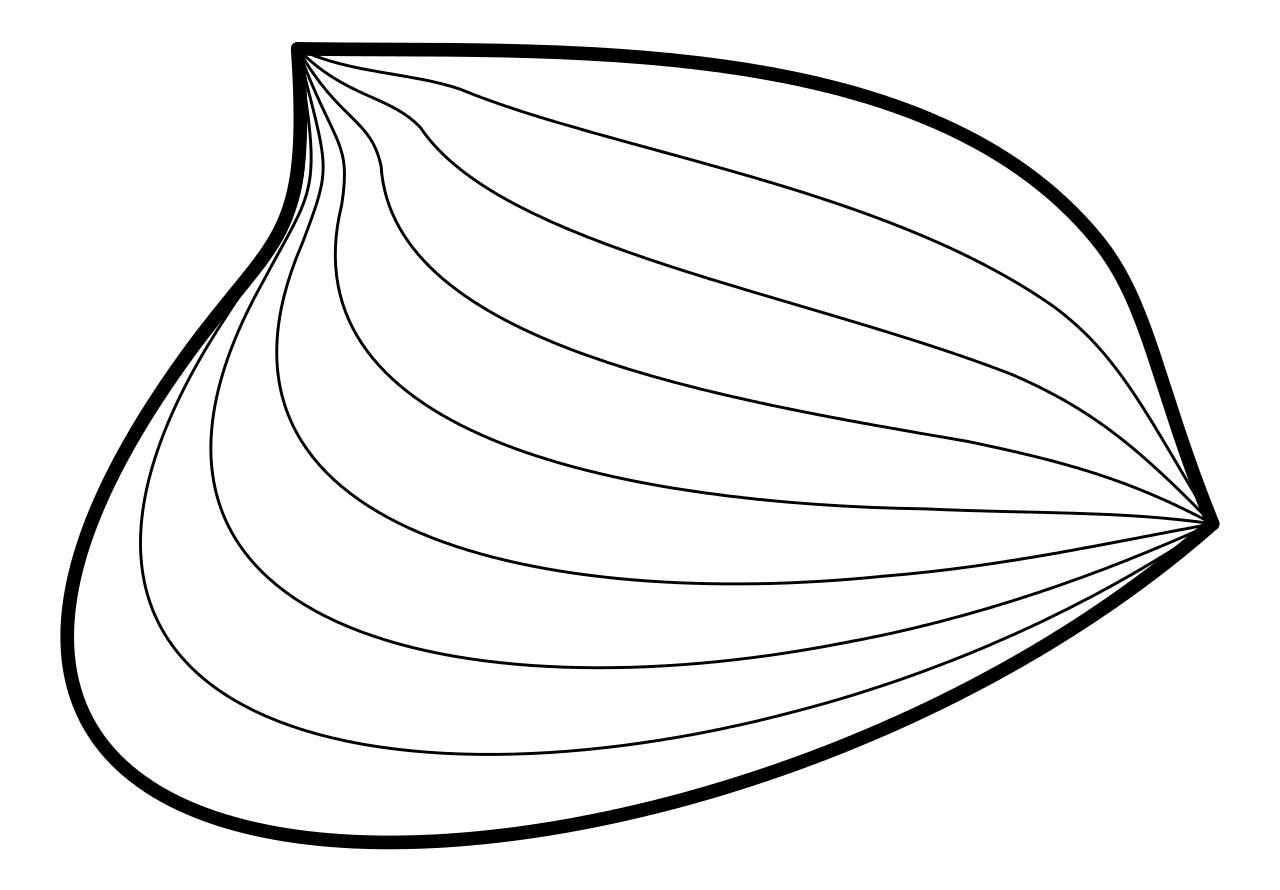
\includegraphics[scale=0.15]{imagens/homotopy.png}

\caption{Ilustração de uma homotopia de caminhos.}
\end{figure}

\begin{proposition}
	Sejam $X$ um espaço métrico e $x_0 \in X$. Então a relação $\approx$ de homotopia de caminhos é uma relação de equivalência em $L(X,x_0)$.
\end{proposition}
\begin{proof} Sejam $l_1,l_2,l_3 \in L(X,x_0)$. Então
	\begin{enumerate}
	\item Reflexividade: $l_1 \approx l_1$. \\
	Consideremos a função
		\begin{align*}
		H: S^1 \times \intff{0}{1} &\to X \\
		(x,t) &\mapsto l(x).
		\end{align*}
Sabemos que $H$ é uma homotopia entre $l_1$ e $l_1$. Basta notar que, para todo $t \in \intff{0}{1}$, $H(0,t)=H(1,t)=l(0)$, o que termina a demonstração de que $H$ é uma homotopia de laços entre $l_1$ e $l_1$.
	
	\item Simetria: $l_1 \approx l_2 \Rightarrow l_2 \approx l_1$. \\
	Seja $H: S^1 \times \intff{0}{1} \to X$ uma homotopia de laços entre $l_1$ e $l_2$. Então consideremos a função
	\begin{align*}
	H': S^1 \times \intff{0}{1} &\to X \\
		(x,t) &\mapsto H(x,1-t).
	\end{align*}		
Sabemos que $H$ é uma homotopia entre $l_2$ e $l_1$. Basta notar que, para todo $t \in \intff{0}{1}$, $H'(0,t)=H(0,1-t)=l(0)=H(1,1-t)=H'(1,t)$, o que termina a demonstração de que $H'$ é uma homotopia de laços entre $l_2$ e $l_1$.

	\item Transitividade: $l_1 \approx l_2 \text{\ \ e\ \ } l_2 \approx l_3 \Rightarrow l_1 \approx l_3$. \\
	Sejam $H_1: S^1 \times \intff{0}{1} \to X$ uma homotopia entre $l_1$ e $l_2$ e $H_2: S^1 \times \intff{0}{1} \to X$ uma homotopia entre $l_2$ e $l_3$. Então consideremos a função
	\begin{align*}
	H: S^1 \times \intff{0}{1} &\to X \\
		(x,t) &\mapsto \begin{cases}
						H_1(x,2t) &\text{se $0 \leq t \leq \frac{1}{2}$}\\
						H_2(x,2t-1) &\text{se $\frac{1}{2} \leq t \leq 1$}.
						\end{cases}
	\end{align*}
Sabemos que $H$ é uma homotopia entre $l_1$ e $l_3$. Basta notar que, como $H_1$ é homotopia de laços, para todo $t \in [0,\frac{1}{2}]$, $H(0,t)=H_1(0,2t)=l_1(0)$ e, como $H_2$ é homotopia de laços entre $l_2$ e $l_3$, para todo $t \in [\frac{1}{2},1]$, $H(0,t)=H_2(0,2t-1)=l_2(0)=l_1(0)$ o que termina a demonstração de que $H$ é uma homotopia de laços entre $l_1$ e $l_3$. 
	\end{enumerate}
\end{proof}

\begin{proposition}
\label{prop:homo}
	Seja $X$ um espaço métrico e $c_1,c_2,c_3: \intff{0}{1} \to X$ caminhos em $X$ tais que $c_1(0)=x_0$, $c_1(1)=c_2(0)$, $c_2(1)=c_3(0)$ e $c_3(0)=x_1$. Então
	\begin{enumerate}
	\item $c_1 \comp (c_1)^{-1} \approx e_{x_0}$;
	\item $(c_1)^{-1} \comp c_1 \approx e_{x_1}$;
	\item $e_{x_0} \comp c_1 \approx c_1 \approx c_1 \comp e_{x_1}$;
	\item $(c_1 \comp c_2) \comp c_3 \approx c_1 \comp (c_2 \comp c_3)$.
	\end{enumerate}
\end{proposition}
\begin{proof}
	\begin{enumerate}
	\item Notemos que
	\begin{equation*}
	c_1 \comp (c_1)^{-1}(s)
		=
			\begin{cases}
				c_1(2s) &\text{se $s \in [0,\frac{1}{2}]$} \\
				(c_1)^{-1}(2s-1) &\text{se $s \in [\frac{1}{2},1]$}.
			\end{cases}
		=
			\begin{cases}
				c_1(2s) &\text{se $s \in [0,\frac{1}{2}]$} \\
				c_1(2-2s) &\text{se $s \in [\frac{1}{2},1]$}.
			\end{cases}
	\end{equation*}
	Assim, considerando a parametrização $\phi: [0,1] \to [0,1]$
	\begin{equation*}
	\phi(s)
		=
			\begin{cases}
				2s &\text{se $s \in [0,\frac{1}{2}]$} \\
				2-2s &\text{se $s \in [\frac{1}{2},1]$}
			\end{cases}
	\end{equation*}
segue que $c_1 \comp (c_1)^{-1}(s) = c_1(\phi(s))$.
Consideremos, assim, a função
	\begin{align*}
	H: [0,1] \times [0,1] &\to X \\
		(s,t) &\mapsto c_1((1-t)\phi(s)).
	\end{align*}
	Temos que $H$ é contínua, pois $c_1$, $1-t$ e $\phi$ são contínuas. Agora, notemos que, para todo $s,t \in [0,1]$, $1-t \in [0,1]$ e $\phi(s) \in [0,1]$, o que mostra que $(1-t)\phi(s) \in [0,1]$ e, portanto, que $H$ está bem definida. Ainda, para todo $s \in [0,1]$, $H(s,0)=c_1(\phi(s))=c_1 \comp (c_1)^{-1}(s)$ e $H(s,1)=c_1(0)=x_0$. Portanto $H$ é homotopia entre $c_1 \comp (c_1)^{-1}$ e $e_{x_0}$.	Para mostrar que $H$ é homotopia de caminhos, note que, para todo $t \in [0,1]$,	$H(0,t)=c_1((1-t)\phi(0))=c_1(0)$ e $H(1,t)=c_1((1-t)\phi(1))=c_1(0)$, o que termina a demonstração.
	
	\item Análogo ao item anterior, mas considerando a parametrização $\phi: [0,1] \to [0,1]$
	\begin{equation*}
	\phi(s)
		=
			\begin{cases}
				1-2s &\text{se $s \in [0,\frac{1}{2}]$} \\
				2s-1 &\text{se $s \in [\frac{1}{2},1]$}.
			\end{cases}
	\end{equation*}
	
	\item Análogo ao item anterior, mas considerando as parametrizações $\phi,\phi': [0,1] \to [0,1]$
	\begin{equation*}
	\phi(s)
		=
			\begin{cases}
				0 &\text{se $s \in [0,\frac{1}{2}]$} \\
				2s-1 &\text{se $s \in [\frac{1}{2},1]$}.
			\end{cases}
	\end{equation*}
	\begin{equation*}
	\phi'(s)
		=
			\begin{cases}
				2s &\text{se $s \in [0,\frac{1}{2}]$} \\
				0 &\text{se $s \in [\frac{1}{2},1]$}.
			\end{cases}
	\end{equation*}
	
	\item Notemos que
	\begin{align*}
	(c_1 \comp c_2) \comp c_3 &=
		\begin{cases}
		c_1 (4s) &\text{se $s \in [0,\frac{1}{4}]$}  \\
		c_2(4s-1) &\text{se $s \in [\frac{1}{4},\frac{1}{2}]$} \\
		c_3(2s-1) &\text{se $s \in [\frac{1}{2},1]$}
		\end{cases} \\
	c_1 \comp (c_2 \comp c_3) &=
		\begin{cases}
		c_1 (2s) &\text{se $s \in [0,\frac{1}{2}]$}  \\
		c_2(4s-2) &\text{se $s \in [\frac{1}{2},\frac{3}{4}]$} \\
		c_3(4s-3) &\text{se $s \in [\frac{3}{4},1]$}.
		\end{cases}
	\end{align*}
	
	Assim, considerando a parametrização $\phi: [0,1] \to [0,1]$
	\begin{equation*}
	\phi(s)
		=
			\begin{cases}
				2s &\text{se $s \in [0,\frac{1}{4}]$} \\
				s + \frac{1}{4} &\text{se $s \in [\frac{1}{4},\frac{1}{2}]$} \\
				\frac{s}{2}+\frac{1}{2} &\text{se $s \in [\frac{1}{2},1]$}.
			\end{cases}
	\end{equation*}	
segue que $((c_1 \comp c_2) \comp c_3)(s) = (c_1 \comp (c_2 \comp c_3)) (\phi(s))$. Consideremos, assim, a função
	\begin{align*}
	H: [0,1] \times [0,1] &\to X \\
		(s,t) &\mapsto (c_1 \comp c_2) \comp c_3 ((1-t)s + t \phi(s)).
	\end{align*}
	Analogamente aos itens anteriores, mostra-se que $H$ é homotopia de caminhos.
	\end{enumerate}
\end{proof}


\begin{proposition}
\label{prop:equiv}
	Sejam $X$ um espaço métrico, $x_0 \in X$ e $c_1,c_2,c'_1,c'_2 : [0,1] \to X$ caminhos em $X$. Então
	\begin{enumerate}
	\item Se $c_1 \approx c'_1$ e $c_2 \approx c'_2$, então $c_1 \comp c_2 \approx c'_1 \comp c'_2$.
	\item $(c_1)^{-1} \approx (c'_1)^{-1}$.
	\end{enumerate}
\end{proposition}
\begin{proof}
	\begin{enumerate}
	\item Seja $H_1$ a homotopia de caminhos entre $c_1$ e $c'_1$ e $H_2$ a homotopia de caminhos entre $c_2$ e $c'_2$. Consideremos a função
	\begin{align*}
	H: [0,1] \times [0,1] &\to X \\
		(s,t) &\mapsto  \begin{cases}
								H_1(2s,t) &\text{se $0 \leq s \leq \frac{1}{2}$} \\
								H_2(2s-1,t) &\text{se $\frac{1}{2} \leq s \leq 1$}.
								\end{cases}
	\end{align*}
	
	Primeiro, notemos que $H$ é uma homotopia entre $c_1$ e $c_2$. Pa Como $H_1$ e $H_2$ são contínuas, basta mostrar que $H$ é contínua nos pontos em que $s=\frac{1}{2}$. Para isso, notemos que, para todo $t \in [0,1]$, $H_1(2\frac{1}{2},t)=H_1(1,t)=c'_1(1)$, pois $H_1$ é homotopia de caminhos, e $H_2(2\frac{1}{2}-1,t) = H_2(0,t) = c_2(0)$, pois $H_2$ é homotopia de caminhos. Assim, segue que as funções nesses pontos são iguais e, portanto, $H$ é contínua. Ainda, para todo $s \in [0,1]$,
	\begin{equation*}
	H(s,0) = \begin{cases}
						H_1(2s,0) = c_1(2s) &\text{se $0 \leq s \leq \frac{1}{2}$} \\
						H_2(2s-1,0) = c_2(2s-1) &\text{se $\frac{1}{2} \leq s \leq 1$},					\end{cases}
	\end{equation*}
o que mostra que $H(s,0)= (c_1 \comp c_2)(s)$, e
	\begin{equation*}
	H(s,0) = \begin{cases}
						H_1(2s,1) = c'_1(2s) &\text{se $0 \leq s \leq \frac{1}{2}$} \\
						H_2(2s-1,1) = c'_2(2s-1) &\text{se $\frac{1}{2} \leq s \leq 1$},					\end{cases}
	\end{equation*}
o que mostra que $H(s,0)= (c'_1 \comp c'_2)(s)$ e, portanto, que $H$ é homotopia.

	Agora, devemos mostrar que $H$ é homotopia de caminhos. Notemos que, para todo $t \in [0,1]$, $H(0,t) = H_1(0,t) = c_1(0) = (c_1 \comp c_2)(0)$, pois $H_1$ é homotopia de caminhos, e $H(1,t) = H_2(1,t) = c'_2(1) = (c'_1 \comp c'_2)(1)$, o que mostra que $H$ é homotopia de caminhos.
	
	\item Seja $H$ uma homotopia de caminhos entre $c_1$ e $c'_1$. Consideremos a função
	\begin{align*}
	H': [0,1] \times [0,1] &\to X \\
		(s,t) &\mapsto H(1-s,t).
	\end{align*}
	Primeiro notemos que $H'$ é uma homotopia entre  $(c_1)^{-1}$ e $(c'_1)^{-1}$. Claramente, $H'$ é contínua, pois $H$ e $1-s$ são contínuas. Ainda, para todo $s \in [0,1]$,
	\begin{equation*}
	H'(s,0)=H(1-s,0)=c_1(1-s)=(c_1)^{-1}(s)
	\end{equation*}
e
	\begin{equation*}
	H'(s,1)=H(1-s,1)=c'_1(1-s)=(c'_1)^{-1}(s),
	\end{equation*}
pois $H$ é homotopia. Assim, mostramos que $H'$ é homotopia entre $(c_1)^{-1}$ e $(c'_1)^{-1}$.
	
	Agora, mostremos que $H'$ é homotopia de caminhos. Para todo $t \in [0,1]$, $H'(0,t)=H(1,t)=c'_1(1)=(c'_1)^{-1}(0)$ e $H'(1,t)=H(0,t)=c_1(0)=(c_1)^{-1}(1)$, pois $H$ é homotopia de caminhos. Assim, mostramos que $H'$ é homotopia de caminhos entre $(c_1)^{-1}$ e $(c'_1)^{-1}$.
	\end{enumerate}
\end{proof}

\subsection{Grupo fundamental}

Como $\approx$ é uma relação de equivalência em $L(X,x_0)$, podemos considerar o espaço quociente $L(X,x_0) / \approx$ das classes de equivalência de laços em $L(X,x_0)$.

\begin{definition}
	Sejam $X$ um espaço métrico conexo por caminhos e $x_0 \in X$. Então o \emph{grupo fundamental} de $X$ com base em $x_0$ é o conjunto
	\begin{equation*}
	\pi_1(X,x_0) := L(X,x_0) / \approx.
	\end{equation*}
\end{definition}

\begin{definition}
	Sejam $X$ um espaço métrico conexo por caminhos. A \emph{composição} de classes de equivalência de laços em $\pi_1(X)$ é a função
	\begin{align*}
	\comp : \pi_1(X) \times \pi_1(X) &\to \pi_1(X) \\
				([l_1],[l_2]) &\mapsto [l_1 \comp l_2].
	\end{align*}
\end{definition}

Notemos que a composição de caminhos está bem definida por causa da proposição \ref{prop:equiv}.

\begin{theorem}
	Sejam $X$ um espaço métrico conexo por caminhos e $x_0 \in X$. Então  $(\pi_1(X),\comp)$ é um grupo.	
\end{theorem}
\begin{proof}
	Segue direto das proposições  \ref{prop:homo} e \ref{prop:equiv}.
\end{proof}


\part{{\scshape Análise}}

\chapter{Espaços Métricos}

\section{Os Espaços Métricos}

\subsection{Métricas}

\begin{defi}
Seja $M$ um conjunto. Uma \emph{métrica} em $M$ é uma função $d: M \times M \to \R$ que satisfaz
	\begin{enumerate}
	\item (Definição Positiva) Para todos $p_0,p_1 \in M$,
		\begin{equation*}
		d(p_0,p_1)=0 \sse p_0=p_1;
		\end{equation*}
	\item (Simetria) Para todos $p_0,p_1 \in M$
		\begin{equation*}
		d(p_0,p_1)=d(p_1,p_0);
		\end{equation*}
	\item (Desigualdade Triangular) Para todos $p_0,p_1,p_2 \in M$,
		\begin{equation*}
		d(p_1,p_3) \leq d(p_1,p_2) + d(p_2,p_3).
		\end{equation*}
	\end{enumerate}
A \emph{distância} de $p_0$ a $p_1$ é o número real $d(p_0,p_1)$.
\end{defi}

\begin{prop}
Sejam $M$ um conjunto e $d$ uma métrica em $M$. Então
	\begin{enumerate}
	\item (Positividade) Para todos $p_0,p_1 \in M$, $d(p_1,p_2) \geq 0$.
	\item (Desigualdade Triangular Generalizada) Para todos $p_0,\ldots,p_n \in M$,
		\begin{equation*}
		d(p_0,p_n) \leq \bigplus_{i=1}^{n-1} d(p_i,p_{i+1})
		\end{equation*}
%	\item Desigualdade Trianguar Alternativa \\
%	$\forall p_1,p_2,p_3 \in M \qquad |d(p_1,p_3)-d(p_2,p_3)| \leq d(p_1,p_2)$.
	\end{enumerate}
\end{prop}
\begin{proof}
	\begin{enumerate}
	\item Sejam $p_1,p_2 \in M$. Da desigualdade triangular e da simetria de $d$, segue que
	\begin{equation*}
	d(p_1,p_1) \leq d (p_1,p_2)+d(p_2,p_1)= 2 d(p_1,p_2),
	\end{equation*}
Mas $d(p_1,_1) = 0$, o que implica $d(p_1,p_1) \geq 0$.
	\item Para $n=1$, seja $p_1 \in M$; então $d(p_1,p_1)=0$ e $\bigplus_{i=1}^{0} d(p_i,p_{i+1})=0$, pois a soma é vazia. Para $n=2$, sejam $p_1,p_2 \in M$; então $d(p_1,p_2)$ e $\bigplus_{i=1}^{1} d(p_i,p_{i+1})=d(p_1,p_2)$, e vale a propriedade. Para $n=3$, sejam $p_1,p_2,p_3 \in M$; então a propriedade é a desigualdade triangulal. Agora, sejam $n \geq 4$, $p_1,\ldots,p_n \in M$ e assumamos que a propriedade vale para todo $k \in \N$, tal que $3 \leq k \leq n-1$. Então
	\begin{equation*}
	d(p_1,p_n) \leq \bigplus_{i=1}^{n-3} d(p_i,p_{i+1})+d(p_{n-2},p_n),
	\end{equation*}
pois essa soma tem $n-1$ termos e vale a hipótese de indução. Pela desigualdade triangular, vale que $d(p_{n-2},p_n) \leq d(p_{n-2},p_{n-1})+d(p_{n-1},p_n)$, e, portanto,
	\begin{align*}
	d(p_1,p_n) &\leq \bigplus_{i=1}^{n-3} d(p_i,p_{i+1})+d(p_{n-2},p_n) \\
			&\leq \bigplus_{i=1}^{n-3} d(p_i,p_{i+1}) + d(p_{n-2},p_{n-1})+d(p_{n-1},p_n) \\
			&= \bigplus_{i=1}^{n-1} d(p_i,p_{i+1}).
	\end{align*}
	\end{enumerate}
\end{proof}

\begin{prop}
	Sejam $M$ um conjunto e $d_0, \dots, d_n$ métricas em $M$. Então a função
	\begin{align*}
		\func{d}{M \times M}{\R}{(p_0,p_1)}{\bigplus_{i=0}^n d_i(p_0,p_1)}
	\end{align*}
é uma métrica em $M$.
\end{prop}
\begin{proof}
	\begin{enumerate}
	\item (Identidade dos Indiscerníveis) Sejam $p_1,p_2 \in M$. Suponhamos que
	\begin{equation*}
	d(p_1,p_2) = \bigplus_{i=1}^n d_i(p_1,p_2) = 0.
	\end{equation*}
Como, para todo $i \in \inte_n$, $d_i(p_1,p_2) \geq 0$, então, para todo $i \in \inte_n$, $d_i(p_1,p_2) = 0$. Logo $p_1=p_2$. Reciprocamente, suponhamos $p_1=p_2$. Então, para todo $i \in \inte_n$, $d_i(p_1,p_2)=0$, o que implica
	\begin{equation*}
	d(p_1,p_2) = \bigplus_{i=1}^n 0 = 0.
	\end{equation*}
	
	\item (Simetria) Sejam $p_1,p_2 \in M$. Então, pela simetria de $d_i$ para todo $i \in \inte_n$,
	\begin{equation*}
	d(p_1,p_2) = \bigplus_{i=1}^n d_i(p_1,p_2) = \bigplus_{i=1}^n d_i(p_2,p_1) = d(p_2,p_1).
	\end{equation*}
	
	\item (Desigualdade Triangular) Sejam $p_1,p_2,p_3 \in M$. Então, para todo $i \in \inte_n$, vale $d_i(p_1,p_3) \leq d_i(p_1,p_2)+d_i(p_2,p_3)$ pela desigualdade triangular de $d_i$, e segue que
	\begin{align*}
	d(p_1,p_3) &= \bigplus_{i=1}^n d_i(p_1,p_3) \\
				&\leq \bigplus_{i=1}^n (d_i(p_1,p_2)+d_i(p_2,p_3)) \\
				&= \bigplus_{i=1}^n d_i(p_1,p_2) + \bigplus_{i=1}^n d_i(p_2,p_3) \\
				&= d(p_1,p_2)+d(p_2,p_3).
	\end{align*}
	\end{enumerate}
\end{proof}

\begin{prop}
	Sejam $M$ um conjunto não vazio e $d_1,d_2$ métricas em $M$. Então a função
	\begin{align*}
	d: M \times M &\to \R \\
	 (p_1,p_2) &\mapsto \max\{d_1(p_1,p_2),d_2(p_1,p_2)\}
	\end{align*}
é uma métrica em $M$.
\end{prop}
\begin{proof}
	\begin{enumerate}
	\item (Definição Positiva) Sejam $p_1,p_2 \in M$. Suponhamos que
	\begin{equation*}
	d(p_1,p_2)=\max\{d_1(p_1,p_2),d_2(p_1,p_2)\}=0.
	\end{equation*}
Então $d_1(p_1,p_2)=0$ ou $d_2(p_1,p_2)=0$. Em ambos os casos, temos $p_1=p_2$. Reciprocamente, suponhamos que $p_1=p_2$. Então $d_1(p_1,p_2)=0$ e $d_2(p_1,p_2)=0$, o que implica $d(p_1,p_2)=\max\{d_1(p_1,p_2),d_2(p_1,p_2)\}=0$.
	
	\item (Simetria) Sejam $p_1,p_2 \in M$. Então
	\begin{equation*}
	d(p_1,p_2) = \max\{d_1(p_1,p_2),d_2(p_1,p_2)\} = \max\{d_1(p_2,p_1),d_2(p_2,p_1)\} = d(p_2,p_1).
	\end{equation*}
	
	\item (Desigualdade Triangular) Sejam $p_1,p_2,p_3 \in M$. Então $d(p_1,p_3)=d_1(p_1,p_3)$ ou $d(p_1,p_3)=d_2(p_1,p_3)$. No primeiro caso, segue que
	\begin{equation*}
	d(p_1,p_3) = d_1(p_1,p_3) \leq d_1(p_1,p_2) + d_1(p_2,p_3) \leq d(p_1,p_2) + d(p_2,p_3).
	\end{equation*}
	No segudo caso, segue que
	\begin{equation*}
	d(p_1,p_3) = d_2(p_1,p_3) \leq d_2(p_1,p_2) + d_2(p_2,p_3) \leq d(p_1,p_2) + d(p_2,p_3).
	\end{equation*}
	\end{enumerate}
\end{proof}

\begin{defi}
Um \emph{espaço métrico} é um par $\bm M=(M,d)$ em que $M$ é um conjunto e $d$ é uma métrica em $M$. Os elementos de $M$ são \emph{pontos}. Um \emph{subespaço métrico} de $\bm M$ é o par $\bm S=(S,d|_{S \times S})$.
\end{defi}

\subsection{Diâmetro, Bolas Abertas e Bolas Fechadas}

\begin{defi}
Sejam $\bm M$ um espaço métrico e $C \subseteq M$ um conjunto não vazio. O \emph{diâmetro} de $C$ é o número
	\begin{equation*}
	\diam(C) \coloneqq \sup(d(C \times C)) = \sup\set{d(p_0,p_1)}{p_0,p_1 \in C}
	\end{equation*}
se $d(C \times C)$ é limitado superiormente, e $\infty$, caso contrário. Um \emph{conjunto limitado em $\bm M$} é um conjunto $C \subseteq M$ tal que $\diam(C) \in \R$. Uma \emph{sequência limitada} em $\bm M$ é uma sequência $(p_n)_{n \in N}$ em $M$ tal que $\set{p_n}{n \in \N}$ é limitado.
\end{defi}

\begin{defi}
Sejam $\bm M$ um espaço métrico, $c \in M$ e $r \in \R$. A \emph{bola aberta} de centro $c$ e raio $r$ em $M$ é o conjunto
	\begin{equation*}
	\bola_r(c) \coloneqq \set{p \in M}{d(c,p) < r}.
	\end{equation*}
A \emph{bola fechada} de centro $c$ e raio $r$ em $M$ é o conjunto
	\begin{equation*}
	\bar\bola_r(c) \coloneqq \set{p \in M}{d(c,p) \leq r}.
	\end{equation*}
\end{defi}

\begin{prop}
Sejam $\bm M$ um espaço métrico e $C \subseteq M$ um conjunto. Então $C$ é um conjunto limitado se, e somente se, existem $c \in M$ e $r \in \R$ tais que $C \subseteq \bola_r(c)$.
\end{prop}

\section{Topologia dos Espaços Métricos}

\subsection{Interior e Pontos Interiores}

\begin{defi}
Sejam $\bm M$ um espaço métrico e $C \subseteq M$ um conjunto. Um \emph{ponto interior} de $C$ é um ponto $p \in C$ para o qual existe um número real $r > 0$ tal que $\bola_r(p) \subseteq C$. O \emph{interior} de $C$ é o conjunto $\inn{C}$ de todos pontos interiores de $C$. Um \emph{conjunto aberto} de $\bm M$ é um conjunto $A \subseteq M$ tal que $A = A^\circ$. O conjunto dos conjuntos abertos de $\bm M$ é denotado $\topo_{\bm M}$.
\end{defi}

\begin{prop}
Seja $\bm M = (M,d)$ um espaço métrico. Então
	\begin{enumerate}
	\item Para todo $c \in M$ e para todo número real $r > 0$, a bola aberta $B_r(c)$ é um conjunto aberto;
	\item O conjunto $\topo_{\bm M}$ é uma topologia de $M$.
	\end{enumerate}
\end{prop}
\begin{proof}
	\begin{enumerate}
	\item Sejam $c \in M$ e $r \in \R_+^*$. Queremos mostrar que $\bola_r(c)$ é aberto. Para isso, seja $p \in \bola_r(c)$. Então segue que $d \coloneqq d(c,p) < r$, pela definição de bola aberta, e, portanto, $r-d \in \R_+^*$. Para mostrar que essa bola centrada em $p$ está contida na bola maior centrada em $c$, seja $p' \in \bola_{r-d}(p)$. Então $d(p,p')<r-d$ e, pela desigualdade triangular, segue que
	\begin{equation*}
	d(c,p') \leq d(c,p) + d(p,p') < D + (r-d) = r,
	\end{equation*}
o que mostra que $p' \in \bola_r(c)$ e que, portanto, $\bola_s(p) \subseteq \bola_r(c)$. Assim, mostramos que $\bola_r(p)$ é aberta.
	
	\item
		\begin{enumerate}
		\item Podemos notar que $\emptyset$ é aberto por vacuidade, pois, se não fosse, existiria $p \in \emptyset$ para o qual não há $r \in \R_+^*$ satisfazendo $\bola_r(p) \subseteq A$, o que é absurdo.
	Para mostrar que $M$ é aberto, sejam $p \in M$ e $r \in \R_+^*$. Então $\bola_r(p) \subseteq M$, pois qualquer bola aberta é subconjunto de $M$. Portanto $M$ é aberto.
	
		\item Seja $(A_i)_{i \in I}$ uma família de abertos em $\bm M$ e seja $p \in (A_i)_{i \in I}$. Então existe $k \in I$ tal que $p \in A_k$. Como $A_k$ é aberto, então existe $r \in \R_+^*$ tal que $\bola_r(p) \subseteq A_k$. Como $A_k \subseteq (A_i)_{i \in I}$, segue que $\bola_r(p) \subseteq (A_i)_{i \in I}$ e que, portanto, $(A_i)_{i \in I}$ é aberto.
	
		\item Seja $(A_i)_{i \in \inte_n}$ uma sequência de abertos em $\bm M$ e seja $p \in (A_i)_{i \in \inte_n}$. Então, para todo $k \in \inte_n$, $p \in A_k$. Como, para todo $k \in \inte_n$, $A_k$ é aberto, segue que existe $r_k \in \R_+^*$ tal que $\bola_{r_k}(p) \subseteq A_k$, Seja $r \coloneqq \min \{r_k : k \in \inte_n\}$. Então, para todo $k \in \inte_n$, vale $\bola_r(p) \subseteq \bola_{r_k}(p)$, e segue que $\bola_r(p) \subseteq A_k$ e, portanto, $\bola_r(p) \subseteq (A_i)_{i \in \inte_n}$, o que mostra que $(A_i)_{i \in \inte_n}$ é aberto.
		\end{enumerate}		
	\end{enumerate}
\end{proof}

\subsection{Limites e Convergência de Sequências}

\begin{defi}
Sejam $\bm M$ um espaço métrico, $(p_n)_{n \in \N}$ uma sequência de pontos em $M$ e $p \in M$. A sequência $(p_n)_{n \in \N}$  \emph{converge} para o ponto $p$ se, e somente se, para todo número real $\varepsilon > 0$, existe um número natural $N$ tal que
	\begin{equation*}
	\forall n \in \N \qquad n \geq N \Rightarrow p_n \in \bola_\varepsilon(p).
	\end{equation*}
Denota-se $(p_n)_{n \in \N} \conv p$. O ponto $p$ é um \emph{limite} da sequência.  Caso contrário, a sequência não converge para $p$. Uma \emph{sequência convergente} é uma sequência que tem limite. Uma sequência \emph{divergente} é uma sequência que não tem limite.
\end{defi}

\begin{prop}
Todo espaço métrico $\bm M$ é um espaço topológico separado.
\end{prop}
\begin{proof}
Sejam $p,p' \in M$ pontos distintos. Mostraremos que existe um número real $r$ tal que $0 < r \leq \frac{1}{2} d(p,p')$, e que isso implica que $\bola_r(p) \cap \bola_r(p') = \emptyset$. Como $p \neq p'$, então $d(p,p') > 0$, portanto existe $r \in \R$ tal que $0 < r \leq \frac{1}{2} d(p,p')$. Suponhamos que existe $p'' \in \bola_r(p) \cap \bola_r(p')$. Então $d(p,p'')<r$ e $d(p',p'')<r$. Mas, pela desigualdade triangular, segue que
	\begin{equation*}
	d(p,p') \leq d(p,p'') + d(p'',p') < r + r \leq d(p,p'),
	\end{equation*}
o que é absurdo. Portanto $\bola_r(p) \cap \bola_r(p') = \emptyset$.
\end{proof}

\begin{coro}
Toda sequência convergente em um espaço métrico $\bm M$ tem limite único.
\end{coro}
\begin{proof}
Suponhamos que $p,p'$ são limites de $(p_n)_{n \in \N}$. Se $p \neq p'$, então $d(p,p')>0$. Seja $\varepsilon \in \R$ tal que $0 < \varepsilon \leq \frac{1}{2} d(p,p')$. Então existe $N_1 \in \N$ tal que, para todo $n \in \N$, se $n \geq N_1$, então $p_n \in \bola_\varepsilon(p)$, e existe $N_2 \in \N$ tal que, para todo $n \in \N$, se $n \geq N_2$, então $p_n \in \bola_\varepsilon(p')$. Assim, definindo $N \coloneqq \max \{N_1,N_2\}$, segue que, se $n \geq N$, então $n \geq N_1$ e $n \geq N_2$, e, portanto, que $p_n \in \bola_\varepsilon(p)$ e $p_n \in \bola_\varepsilon(p')$; ou seja, $p_n \in \bola_\varepsilon(p) \cap \bola_\varepsilon(p')$, mas isso é absurdo, pois $\bola_\varepsilon(p) \cap \bola_\varepsilon(p')=\emptyset$. Portanto $p=p'$.
\end{proof}

Essa proposição nos permite tratar o limite de uma sequência como um número único e, por isso, podemos usar a notação $\displaystyle\lim_{n \in \N} p_n = p$ para quando $(p_n)_{n \in \N} \conv p$.

\begin{prop}
Uma sequência de em um espaço métrico $\bm M$ é convergente se, e somente se, todas suas subsequências são convergentes.
\end{prop}
\begin{proof}
	Suponhamos que $(p_n) \conv p$ e seja $(p_{n_k})_{k \in \N}$ uma subsequência de $(p_n)_{n \in \N}$. Seja $\varepsilon \in \R$ tal que $\varepsilon > 0$. Como $(p_n) \conv p$, existe $N \in \N$ tal que, para todo $n \in \N$, se $n \geq N$, então $p_n \in \bola_\varepsilon(p)$; como $(n_k)_{k \in \N}$ é estritamente crescente, existe $K \in \N$ tal que, para todo $k \in \N$, se $k \geq K$, então $n_k \geq N$. Mas então
	\begin{equation*}
	k \geq K \Rightarrow n_k \geq N \Rightarrow p_{n_k} \in \bola_\varepsilon(p)
	\end{equation*}
e, portanto, $(p_{n_k}) \to p$.	Reciprocamente, se toda subsequência de $(p_n)_{n \in \N}$ converge para $p$, $(p_n)_{n \in \N}$, em particular, é uma dessas subsequências e, portanto, $(p_n) \conv p$.
\end{proof}

\begin{prop}
Toda sequência convergente em um espaço métrico $\bm M$ é limitada.
\end{prop}
\begin{proof}
	Seja $(p_n)_{n \in \N}$ uma sequência de pontos em $M$ tal que $(p_n) \conv p$. Então, para $\varepsilon = 1$, existe $N \in \N$ tal que, para todo $n \in \N$, se $n \geq N$, então $p_n \in \bola_1(p)$. Assim, seja $l \in \R$ tal que
	\begin{equation*}
	l > \max(\{1\} \cup \{d(p,p_n) : n \in \inte_N\}),
	\end{equation*}
seque que, para todo $n \in \N$, $p_n \in \bola_l(p)$ pois, se $0 \leq n \leq N$, $d(p,p_n) < l$ pela definição de $l$ e, se $n \geq N$, então $p_n \in \bola_1(p) \subseteq B_l(p)$, pois $1 < l$. Logo $(p_n)_{n \in \N}$ é limitada.
\end{proof}

\begin{prop}
Sejam $\bm M$ um espaço métrico, $C \subseteq M$ um conjunto e $p \in M$. Então existe uma sequência de pontos em $C$ que converge para $p$ se, e somente se, para todo número real $\varepsilon > 0$, $C \cap \bola_\varepsilon(p) \neq \emptyset$.
\end{prop}
\begin{proof}
	Suponhamos que exista uma sequência $(p_n)_{n \in \N}$ de pontos em $C$ tal que $(p_n) \conv p$. Então, para todo número real $\varepsilon > 0$, existe $N \in \N$ tal que, para todo $n \in \N$, se $n \geq N$, então $p_n \in \bola_\varepsilon(p)$. Mas isso implica que $p_n \in C \cap \bola_\varepsilon(p)$. Reciprocamente, suponhamos que, para todo número real $\varepsilon > 0$, $C \cap \bola_\varepsilon(p) \neq \emptyset$. Então, em particular, para todo $n \in \N$, escolhamos $p_n \in C \cap \bola_{\frac{1}{n}}(p)$. Assim, temos a sequência $(p_n)_{n \in \N}$. Para mostrar que $(p_n) \conv p$, seja $\varepsilon \in \R$ tal que $\varepsilon > 0$. Então existe $N \in \N$ tal que $\frac{1}{N} \leq \varepsilon$. Mas isso implica que, para todo número natural $n \geq N$, $\frac{1}{n} \leq \frac{1}{N}$, e segue que
	\begin{equation*}
	d(p,p_n) < \frac{1}{n} \leq \frac{1}{N} \leq \varepsilon
	\end{equation*}
e, portanto, $(p_n) \conv p$.
\end{proof}

\begin{prop}
Sejam $\bm M$ um espaço métrico, $p,q \in M$ e $(p_n)_{n \in \N}$ e $(q_n)_{n \in \N}$ sequências em $M$ que convergem para $p$ e $q$ respectivamente. Então a sequência $(d(p_n,q_n))_{n \in \N}$ em $\R$ converge para $d(p,q)$.
\end{prop}
\begin{proof}
	Para todo $n \in \N$, segue da desigualdade triangular que
	\begin{equation*}
	d(p_n,q_n) \leq d(p_n,p) + d(p,q) + d(q,q_n).
	\end{equation*}
Seja $\varepsilon > 0$ um número real. Então existem $N_1,_2 \in \N$ tais que
	\begin{equation*}
	\forall n \in \N \qquad n \geq N_1 \Rightarrow d(p,p_n) < \frac{\varepsilon}{2}
	\end{equation*}
e
	\begin{equation*}
	\forall n \in \N \qquad n \geq N_2 \Rightarrow d(q,q_n) < \frac{\varepsilon}{2}.
	\end{equation*}
Fazendo $N_3 \coloneqq \max\{N_1,N_2\}$, segue que
	\begin{equation*}
	\forall n \in \N \qquad n \geq N_3 \Rightarrow d(p_n,q_n) \leq d(p_n,p) + d(p,q) + d(q,q_n) < d(p,q) + \varepsilon;
	\end{equation*}
ou seja, $d(p_n,q_n) - d(p,q) < \varepsilon$. Analogamente, achamos $N_6 \in \N$ tal que
	\begin{equation*}
	\forall n \in \N \qquad n \geq N_3 \Rightarrow d(p_n,q_n) \leq d(p_n,p) + d(p,q) + d(q,q_n) < d(p,q) + \varepsilon
	\end{equation*}
e fazendo $n \coloneqq \max\{N_3,N_6\}$, segue que
	\begin{equation*}
	\forall n \in \N \qquad n \geq N \Rightarrow |d(p,q) - d(p_n,q_n)| < \varepsilon,
	\end{equation*}
o que mostra que $(d(p_n,q_n)) \conv d(p,q)$ em $\R$.
	
\end{proof}

\subsection{Fecho e Pontos Aderentes}

\begin{defi}
Sejam $\bm M$ um espaço métrico e $C \subseteq M$ um conjunto. Um \emph{ponto aderente} a $C$ é um ponto $p \in M$ para o qual existe uma sequência $(p_n)_{n \in \N}$ de pontos de $C$ que converge para $p$. O \emph{fecho} de $C$ é o conjunto $\fec{C}$ de todos os pontos aderentes a $C$. Um \emph{conjunto fechado} de $\bm M$ é um conjunto $F \subseteq M$ tal que $F = \fec{F}$.
\end{defi}

\begin{prop}
Sejam $\bm M$ um espaço métrico e $F \subseteq M$. Então $F$ é um conjunto fechado se, e somente se, $F^\complement$ é um conjunto aberto.
\end{prop}
\begin{proof}
Suponhamos que $F$ é um conjunto fechado. Se $F^\complement = \emptyset$, Mas $\emptyset$ é aberto pois, caso contrário, existe $p \in \emptyset$ para o qual não há número real $\varepsilon > 0$ tal que $\bola_\varepsilon(p) \subseteq \emptyset$, mas isso é absurdo. Se $F^\complement \neq \emptyset$, seja $p \in F^\complement$. Se não existe número real $\varepsilon > 0$ tal que $\bola_\varepsilon(p) \subseteq F^\complement$, então, para todo número real $\varepsilon > 0$, $F \cap \bola_\varepsilon(p) \neq \emptyset$. Mas isso implica que existe uma sequência $(p_n)_{n \in \N}$ de pontos em $F$ tal que $(p_n) \conv p$. Como $F$ é fechado, isso implica $p \in F$, o que é uma contradição. Então existe número real $\varepsilon > 0$ tal que $\bola_\varepsilon(p) \subseteq F^\complement$, e isso mostra que $F^\complement$ é aberto.
	
Reciprocamente, suponhamos que $F^\complement$ é aberto. Se $F = \emptyset$, então $F$ é fechado. Se $F \neq \emptyset$, seja $(p_n)_{n \in \N}$ uma sequência em $F$ que converge para $p \in M$. Suponhamos que $p \notin F$. Então $p \in F^\complement$ e, como $F^\complement$ é aberto, existe um número real $\varepsilon > 0$ tal que $\bola_\varepsilon(p) \subseteq F^\complement$. Como $(p_n) \conv p$, existe $N \in \N$ tal que, para todo $n \in \N$, se $n \geq N$, então $p_n \in \bola_\varepsilon(p)$. Mas isso implica que $p_N \in \bola_\varepsilon(p) \subseteq F^\complement$, o que é absurdo, pois $p_n \in F$. Portanto $p \in F$ e isso mostra que $F$ é fechado.
\end{proof}

\begin{prop}
Seja $\bm M$ um espaço métrico. Então, para todo $c \in M$ e para todo número real $r > 0$, a bola fechada $\bar\bola_r(c)$ é um conjunto fechado.
\end{prop}
\begin{proof}
Basta notar que $\bar\bola_r(c)^\complement$ é aberto.
\end{proof}

\subsection{Continuidade}

\begin{defi}
Sejam $\bm M_1$ e $\bm M_2$ espaços métricos, $f: M_1 \to M_2$ uma função e $p \in M$. A função $f$ é \emph{contínua em $p$} se, para todo número real $\varepsilon > 0$, existe um número real $\delta > 0$ tal que
%	\begin{equation*}
%	\forall x \in M_1 \qquad d_1(p,x) < \delta \Rightarrow d_2(f(p),f(x)) < \varepsilon.
%	\end{equation*}
	\begin{equation*}
	\forall x \in M_1 \qquad x \in \bola_\delta(p) \Rightarrow f(x) \in \bola_\varepsilon(f(p)).
	\end{equation*}
Caso contrário, a função $f$ não é contínua em $p$, ela é \emph{descontínua} em $p$.
\end{defi}

Denotamos as bolas abertas em $\bm M_1$ e em $\bm M_2$ por $\bola$, mas deve-se perceber que elas são relativas a métricas possivelmente diferentes. 

\begin{prop}
Sejam $\bm M_1$ e $\bm M_2$ espaços métricos, $f: M_1 \to M_2$ uma função e $p \in M_1$. Então $f$ é contínua em $p$ se, e somente se, para toda sequência $(p_n)_{n \in \N}$ de pontos em $M_1$ que converge para $p$, a sequência $(f(p_n))_{n \in \N}$ de pontos em $M_2$ converge para $f(p)$; ou seja
	\begin{equation*}
	\lim f(p_n) = f(\lim p_n).
	\end{equation*}
\end{prop}
\begin{proof}
	Suponhamos que $f$ é contínua em $p$. Seja $(p_n)_{n \in \N}$ uma sequência de pontos em $M_1$ que converge para $p$. Seja um número real $\varepsilon > 0$. Como $f$ é contínua, existe um número real $\delta > 0$ tal que $p_n \in \bola_\delta(p)$ implica $f(p_n) \in \bola_\varepsilon(f(p))$. Mas, como $(p_n) \conv p$, existe $N \in \N$ tal que
	\begin{equation*}
	\forall n \in \N \qquad n \geq N \Rightarrow p_n \in \bola_\delta(p) \Rightarrow f(p_n) \in \bola_\varepsilon(f(p))
	\end{equation*}
o que mostra que $(f(p_n)) \conv f(p)$.
	
	Reciprocamente, suponhamos que, para toda sequência $(p_n)_{n \in \N}$ em $M_1$ que converge para $p$, a sequência $(f(p_n))_{n \in \N}$ converge para $f(p)$. Suponhamos, por absurdo, que $f$ não é contínua em $p$. Então existe um número real $\varepsilon > 0$ tal que, para todo número real $\delta > 0$, existe $x \in M_1$ tal que $x \in \bola_\delta(p)$, mas $f(x) \notin \bola_\varepsilon(f(p))$. Vamos mostrar que isso implica que existe uma sequência $(p_n)_{n \in \N}$ em $M_1$ que converge para $p$, mas que a sequência $(f(p_n))_{n \in \N}$ não converge para $f(p)$; ou seja, que existe um número real $\varepsilon > 0$ tal que, para todo número natural $N$, existe $n \in \N$ tal que $n \geq N$, mas $f(p_n) \notin \bola_\varepsilon(f(p))$. Seja $n \in \N$ e tomemos $\delta = \frac{1}{n}$. Então existe $x \in M_1$ tal que $x \in \bola_\frac{1}{n}(p)$, mas $f(x) \notin \bola_\varepsilon(f(p))$. Nomeando esse $x \in M_1$ de $p_n$, obtemos uma sequência $(p_n)_{n \in \N}$ que converge para $p$ pois, para todo número real $\varepsilon' > 0$, existe um número natural $N \in \N$ tal que $\frac{1}{N} \leq \varepsilon'$ e isso implica que
\begin{equation*}
	\forall n \in \N \qquad n \geq N \Rightarrow \frac{1}{n} \leq \frac{1}{N} \leq \varepsilon' \Rightarrow p_n \in \bola_\frac{1}{n}(p) \subseteq \bola_\frac{1}{N}(p) \subseteq \bola_{\varepsilon'}(p).
	\end{equation*}
	No entanto, $(f(p_n))_{n \in \N}$ é uma sequência que não converge para $f(p)$ pois, considerando o $\varepsilon$ original tomado da descontinuidade de $f$, para todo número natural $N$, $f(p_N) \notin \bola_\varepsilon(f(p))$ e isso contradiz a hipótese de que, para toda sequência $(p_n)_{n \in \N}$ em $M_1$ que converge para $p$, a sequência $(f(p_n))_{n \in \N}$ converge para $f(p)$. Portanto $f$ é contínua.	
\end{proof}

\begin{defi}
Sejam $\bm M_1$ e $\bm M_2$ espaços métricos, $D \subseteq M_1$ e $f: D \to M_2$ uma função. A função $f$ é \emph{contínua} em $D$ se ela é contínua em todo ponto de $D$. Caso contrário, a função $f$ é \emph{descontínua} em $D$. Para $D=M_1$, dizemos simplesmente que $f$ é contínua ou descontínua.
\end{defi}

\subsection{Outras Definições}

\begin{defi}
Sejam $\bm M$ um espaço métrico e $C \subseteq M$ um conjunto. Um \emph{ponto limite} (ou \emph{ponto de acumulação}) de $C$ é um ponto $p \in M$ para o qual existe uma sequência $(p_n)_{n \in \N}$ de pontos de $C \setminus \{p\}$ que converge para $p$. O \emph{derivado} de $C$ é o conjunto de todos os pontos limites de $C$. 
\end{defi}

Da definição, segue que $C' \subseteq \overline C$. A inclusão contrária caracteriza a seção a seguir.

\begin{defi}
Sejam $\bm M$ um espaço métrico e $C \subseteq M$ um conjunto. Um \emph{ponto isolado} de $C$ é um ponto $p \in M$ que é um ponto aderente a $C$ mas que não é um ponto limite de $C$.
\end{defi}

Um ponto isolado de $C$ é um ponto $p \in \overline C \setminus C'$.

\section{Isometrias}

\begin{defi}
Sejam $\bm{M_1}$ e $\bm{M_2}$ espaços métricos. Uma \emph{isometria} de $\bm{M_1}$ para $\bm{M_2}$ é uma função $f: M_1 \to M_2$ que satisfaz, para todos $p,p' \in M_1$,
	\begin{equation*}
	d_1(p,p') = d_2(f(p),f(p')).
	\end{equation*}
\end{defi}

\begin{prop}
Toda isometria é injetiva.
\end{prop}

\section{Estrutura Uniforme}

\subsection{Sequências Aproximantes}

\begin{defi}
Seja $\bm M$ um espaço métrico. Uma sequência \emph{aproximante} em $\bm M$ é uma sequência $(p_n)_{n \in \N}$ de pontos em $M$ tal que, para todo número real $\varepsilon > 0$, existe um número natural $N$ satisfazendo
	\begin{equation*}
	\forall n,m \in \N \qquad n,m \geq N \Rightarrow d(p_n,p_m) < \varepsilon.
	\end{equation*}
\end{defi}

Essa sequências são conhecidas como \emph{sequências de Cauchy}. O nome aproximante se dá pelo fato de que os termos da sequência ficam cada vez mais próximos entre si, e será adotado por ser mais intuitivo, embora não seja a nomenclatura padrão.

\begin{prop}
Toda sequência convergente em um espaço métrico $\bm M$ é aproximante.
\end{prop}
\begin{proof}
Seja $(p_n)_{n \in \N}$ uma sequência em $M$ que converge para $p$. Seja $\varepsilon \in \R$ tal que $\varepsilon > 0$. Então $\frac{1}{2}\varepsilon > 0$ é um número real e segue que existe $N \in \N$ tal que, para todo número natural $n \geq N$, $p_n \in \bola_{\frac{1}{2}\varepsilon}(p)$. Assim, segue que	
	\begin{equation*}
	\forall n,m \in \N \qquad n,m \geq N \Rightarrow d(p_n,p_m) \leq d(p_n,p) + d(p,p_m) < \frac{\varepsilon}{2} + \frac{\varepsilon}{2} = \varepsilon,
	\end{equation*}
o que mostra que $(p_n)_{n \in \N}$ é uma sequência aproximante.
\end{proof}

\begin{prop}
Toda sequência aproximante em um espaço métrico $\bm M$ que tem uma subsequência convergente é convergente.
\end{prop}
\begin{proof}
	Seja $(p_{n_k})_{k \in \N}$ uma subsequência de $(p_n)_{n \in \N}$ que converge  para $p$. Seja $\varepsilon > 0$ um número real. Como $(p_n)_{n \in \N}$ é uma sequência de Cauchy e $\frac{1}{2}\varepsilon > 0$ é um número real, existe um número natural $N$ tal que
	\begin{equation*}
	\forall n,m \in \N \qquad n,m \geq N \Rightarrow d(p_n,p_m) < \frac{\varepsilon}{2}.
	\end{equation*}
Como $(p_{n_k})_{k \in \N}$ é uma subsequência convergente, existe $K_1 \in \N$ tal que
	\begin{equation*}
	\forall k \in \N \qquad k \geq K_1 \Rightarrow d(p,p_{n_k}) < \frac{\varepsilon}{2}.
	\end{equation*}
Como $(n_k)_{k \in \N}$ é uma sequência estritamente crescente, existe $K_2 \in \N$ tal que, para todo número natural $k \geq K_2$, $n_k \geq N$. Assim, tomando $K \coloneqq \max\{K_1,K_2\}$, segue que, para todo número natural $n \in \N$, existe $k \in \N$ tal que $n_k \geq N$ e,  pela desigualdade triangular, que
	\begin{equation*}
	\forall n \in \N \qquad n \geq N \Rightarrow d(p_n,p) \leq d(p_n,p_{n_k}) + d(p_{n_k},p) < \frac{\varepsilon}{2}+\frac{\varepsilon}{2}=\varepsilon.
	\end{equation*}
\end{proof}

\begin{prop}
Toda sequência aproximante em um espaço métrico $\bm M$ é limitada.
\end{prop}
\begin{proof}
Seja $(p_n)_{n \in \N}$ uma sequência aproximante em $\bm M$. Então, para $\varepsilon=1$, existe $N \in \N$ tal que
	\begin{equation*}
	\forall n,m \in \N \qquad n,m \geq N \Rightarrow d(p_n,p_m)<1.
	\end{equation*}
	Definamos $P \coloneqq \{p_n : n \in \N\}$. Então segue que
	\begin{align*}
	\diam(P) &= \sup \set{d(p_n,p_m)}{n,m \in \N} \\
		&= \max\{1 \cup \set{d(p_n,p_m)}{0 \leq n,m \leq N}\} \in \R,
	\end{align*}
o que mostra que $(p_n)_{n \in \N}$ é limitada.
\end{proof}

\subsection{Continuidade Uniforme}

\begin{defi}
Sejam $\bm M_1$ e $\bm M_2$ espaços métricos. Uma função \emph{uniformemente contínua} é uma função $f: M_1 \to M_2$ tal que, para todo número real $\varepsilon > 0$, existe um número real $\delta > 0$ tal que
	\begin{equation*}
	\forall p_1,p_2 \in M_1 \qquad d_1(p_1,p_2) < \delta \Rightarrow d_2(f(p_1),f(p_2)) < \varepsilon.
	\end{equation*}
\end{defi}

\begin{prop}
Sejam $\bm M_1$ e $\bm M_2$ espaços métricos, $f: M_1 \to M_2$ uma função uniformemente contínua e $(p_n)_{n \in \N}$ uma sequência aproximante em $M_1$. Então a sequência $(f(p_n))_{n \in \N}$ em $M_2$ é aproximante.
\end{prop}
\begin{proof}
Seja $\varepsilon > 0$ um número real. Da continuidade uniforme de $f$, existe um número real $\delta > 0$ tal que, para todo $p,p' \in M_1$, $d_1(p,p') < \delta$ implica $d_2(f(p),f(p')) < \varepsilon$. Como $(p_n)_{n \in \N}$ é sequência aproximante, existe $N \in \N$ tal que
	\begin{equation*}
	\forall n,m \in \N \qquad n,m \geq N \Rightarrow d_1(p_n,p_m) < \delta.
	\end{equation*}
Mas, da continuidade uniforme de $f$, isso implica que
	\begin{equation*}
	\forall n,m \in \N \qquad n,m \geq N \Rightarrow d_1(p_n,p_m) < \delta  \Rightarrow d_2(f(p_n),f(p_m)) < \varepsilon,
	\end{equation*}
e isso mostra que $(f(p_n))_{n \in \N}$ é uma sequênca aproximante.
\end{proof}

\subsection{Espaços Métricos Completos}

\begin{defi}
Um espaço métrico \emph{completo} é um espaço métrico em que todas sequências aproximantes convergem.
\end{defi}

\begin{prop}
Seja $\bm M$ um espaço métrico. Todo subespaço completo de $\bm M$ é um conjunto fechado em $\bm M$.
\end{prop}
\begin{proof}
Sejam $\bm C \subseteq \bm M$ subsepaço métrico completo e $(p_n)_{n \in \N}$ uma sequência convergente em $C$. Então $(p_n)_{n \in \N}$ é aproximante e, como $C$ é completo, converge para um ponto em $C$, o que significa que $C$ é fechado.
\end{proof}

\begin{prop}
Sejam $\bm M$ um espaço métrico, $\bm C \subseteq \bm M$ um subespaço completo e $F \subseteq C$ um conjunto fechado em $\bm M$. Então $\bm F$ é completo.
\end{prop}
\begin{proof}
Seja $(p_n)_{n \in \N}$ uma sequência aproximante em $F$. Então $(p_n)_{n \in \N}$ é uma sequência aproximante em $C$ e, como $C$ é completo, $(p_n)_{n \in \N}$ converge. Porém, como $F$ é fechado, então $(p_n)_{n \in \N}$ converge para um ponto em $F$, o que mostra que $F$ é completo.
\end{proof}

\begin{teo}
Seja $\bm M$ um espaço métrico. Então $\bm M$ é completo se, e somente se, para toda sequência descrescente $(F_n)_{n \in \N}$ de conjuntos não vazios e fechados em $\bm M$ tais que $(\diam(F_n))_{n \in \N} \conv 0$ em $\R$, vale que
	\begin{equation*}
	\bigcap_{n \in \N} A_n \neq \emptyset.
	\end{equation*}
\end{teo}

\begin{teo}
Sejam $\bm M_1$  um espaço métrico, $\bm M_2$ espaço métrico completo, $D \subseteq M_1$ um conjunto denso em $M_1$ e $f: D \to M_2$ uma função uniformemente contínua. Então $f$ tem uma única extensão para uma função uniformemente contínua $f^*: M_1 \to M_2$. Ainda, se $f$ é uma isometria, então $f^*$ é uma isometria.
\end{teo}
\begin{proof}
	Seja $p \in M_1$. Como $D$ é denso em $M_1$, existe uma sequência $(p_n)_{n \in \N}$ em $D$ que converge para $p$. Como $(p_n)_{n \in \N}$ é convergente, é uma sequência de Cauchy e, como $f$ é uniformemente contínua em $D$, segue que $(f(p_n))_{n \in \N}$ é uma sequência de Cauchy em $M_2$. Mas $M_2$ é completo, o que implica que $(f(p_n))_{n \in \N}$ converge para um ponto $p' \in M_2$. Definimos, portanto, a função $f^*$ em $p$ como $f^*(p)=p'$. Precisamos mostrar que $f^*$ independe da escolha da sequência em $D$ que converge para $p$. Se $(q_n)_{n \in \N}$ é uma sequência em $D$ que converge para $p$, definamos a sequência $(r_n)_{n \in \N}$ em $D$ por
	\begin{equation*}
	r_n \coloneqq
			\begin{cases}
			p_n &\text{se $n=2k$}\\
			q_n &\text{se $n=2k+1$}.
			\end{cases}
	\end{equation*}
A sequência $(r_n)_{n \in \N}$ converge para $p$ e, portanto, é uma sequência de Cauchy. A continuidade uniforme de $f$ implica que a sequência $(f(r_n))_{n \in \N}$ é de Cauchy e, portanto, como $(f(p_n))_{n \in \N}=(f(r_{2k}))_{k \in \N}$ é uma subsequência que converge para $p'$, a sequência $(f(r_n))_{n \in \N}$ converge para $p'$, o que implica que a subsequência $(f(q_n))_{n \in \N}=(f(r_{2k+1}))_{k \in \N}$ converge para $p'$. Assim, mostramos que $f^*$ está bem definida. Claramente, se $p \in D$, então $f(p)=f^*(p)$, pois, como $D$ é denso em $M_1$, se $(p_n)_{n \in \N}$ é uma sequência em $D$ que converge para $p$, então, como $f$ é contínua, segue que $f(p_n) \conv f(p)$, o que mostra que $f^*(p)=f(p)$.

	Agora, devemos mostrar que $f^*$ é uniformemente contínua. Seja $\varepsilon > 0$ um número real, então $\frac{1}{2}\varepsilon > 0$ é um número real e, como $f$ é uniformemente contínua, existe número real $\delta > 0$ tal que
	\begin{equation*}
	\forall p,p' \in M_1 \qquad d_1(p,p') < \delta \Rightarrow d_2(f(p),f(p')) < \frac{\varepsilon}{2}.
	\end{equation*}
Assim, sejam $p,q \in M_1$ tais que $d_1(p,q) < \delta$. Quremos mostrar que $d_2(f(p),f(p')) < \varepsilon$. Sejam $(p_n)_{n \in \N}$ e $(q_n)_{n \in \N}$ sequências que convergem para $p$ e $q$, respectivamente. Então $d_1(p_n,q_n) \conv d_1(p,q)$ em $\R$.

...

	A unicidade de $f^*$ ocorre pois, se existem $f^*$ e $f'^*$ uniformemente contínuas que extendem $f$, como $D$ é denso em $M_1$ e $f^*|_D = f'^*|_D$, segue que $f^* = f'^*$ .
	
	Por fim, mostramos que a isometria se preserva...
\end{proof}

\begin{defi}
Seja $\bm M_1$  um espaço métrico. Um \emph{completamento} de $\bm M$ é um espaço métrico $\bm M_2$ completo tal que $M_1$ é denso em $M_2$.
\end{defi}

\begin{prop}
Seja $\bm M$ um espaço métrico e $\bm M_1$ e $\bm M_2$ completamentos de $\bm M$. Então existe uma isometria entre $\bm M_1$ e $\bm M_2$ que é a função identidade quando restrita a $M$.
\end{prop}
\begin{proof}
	Seja $f$ a função identidade em $M$. Pela proposição anterior, existe uma única extensãouniformemente contínua de $f^*$ em $M_1$ ...
	
	...
\end{proof}


\begin{prop}
Sejam $K \subseteq M$ compacto e $f: M \to \bar M$ contínua. Então $f$ é uniformemente contínua.
\end{prop}
\begin{proof}
Suponhamos, por absurdo, que $f$ não é uniformemente contínua. Então existem $\varepsilon > 0$ e $(x_n)_{n \in \N},(y_n)_{n \in \N}$ sequências em $K$ tais que
	\begin{equation*}
	\nor{x_n - y_n} < \frac{1}{n} \e \nor{f(x_n)-f(y_n)} \geq \varepsilon.
	\end{equation*}
Como $K$ é compacto, existem subsequências $(x_{n_k})_{k \in \N}$  e $(y_{n_k})_{k \in \N}$ convergindo a $x \in K$ com $\nor{f(x_{n_k})-f(y_{n_k})} \geq \varepsilon$. Por continuidade de $f$, existe $\delta > 0$ tal que, se $x_{n_k},y_{n_k} \in B(x,\delta)$, então $\nor{f(x_{n_k})-f(x)} < \frac{\varepsilon}{2}$ e $\nor{f(y_{n_k})-f(x)} < \frac{\varepsilon}{2}$. Pela desigualdade triangular, temos um absudo.
\end{proof}



\chapter{Espaços Normados}

\section{Normas}

\begin{defi}
Seja $\bm E$ um espaço vetorial sobre um corpo $\bm C \subseteq \C$. Uma \emph{norma} em $\bm E$ é uma função $\nor{\cdot}: E \to \R$
que satisfaz
	\begin{enumerate}
	\item (Homogeneidade absoluta) Para todos $c \in C$ e $v \in E$,
		\begin{equation*}
		\nor{a v} = \abs{a}\nor{v};
		\end{equation*}
	\item (Subaditividade) Para todos $v_0,v_1 \in E$,
		\begin{equation*}
		\nor{v_0 + v_1} \leq \nor{v_0} + \nor{v_1};
		\end{equation*}
	\item (Definição positiva) Se $\nor{v}=0$, então $v=0$.
	\end{enumerate}
\end{defi}

Claramente $\abs{\cdot}: \C \to \R$ é uma norma em $\C$.

\begin{prop}
Sejam $\bm E$ um espaço vetorial sobre um corpo $\bm C \subseteq \C$ e $\nor{\cdot}$ uma norma em $\bm E$. Então
	\begin{enumerate}
	\item $\nor{0}=0$;
	\item Para todo $v \in E$, $\nor{-v}=-\nor{v}$;
	\item Para todo $v \in E$, $\nor{v} \geq 0$.
	\item (Subaditividade generalizada) Sejam $v_0,\dots,v_{n-1} \in E$. Então
		\begin{equation*}
		\nor{\bigplus_{0\leq i < n} v_i} \leq \bigplus_{0\leq i < n}\nor{v_i}
		\end{equation*}
	\end{enumerate}
\end{prop}

\begin{defi}
Um \emph{espaço normado} é um par $\E = (\bm E,\nor{\cdot})$ em que $\bm E$ é um espaço vetorial sobre um corpo $\bm C \subseteq \C$ e $\nor{\cdot}$ é uma norma em $\bm E$. A dimensão de $\E$ é a dimensão do espaço vetorial $\bm E$.
\end{defi}

\begin{prop}
Seja $\E$ um espaço normado. A função
	\begin{align*}
	\func{d}{E \times E}{\R}{(v_0,v_1)}{\nor{v_0 - v_1}}.
	\end{align*}
é uma métrica em $E$.
\end{prop}
\begin{proof}
(Definição positiva) Sejam $v,\bar v \in E$. Se $v = \bar v$, então segue da positividade que
	\begin{equation*}
	d(v,\bar v) = d(v,v) = \nor{v - v} = \nor{v-v}=\nor{0}=0.
	\end{equation*}
Reciprocamente, se $d(v,\bar v)=0$, então $\nor{v-\bar v}=0$. Segue da definição positiva $v-\bar v=0$, logo $v=\bar v$.
(Simetria)  Sejam $v,\bar v \in E$. Então segue da homogeneidade absoluta que
	\begin{equation*}
	d(v,\bar v)=\nor{v-\bar v}=\nor{-1(\bar v -v)}=\abs{-1}\nor{\bar v - v}=d(\bar v,v).
	\end{equation*}
(Desigualdade triangular) Sejam $v_0,v_1,v_2 \in E$. Então segue da subaditividade que
	\begin{align*}
	d(v_0,v_2) &= \nor{v_0-v_2} \\
		&=\nor{v_0-v_1+v_1-v_2} \\
		&\leq \nor{v_0-v_1}+\nor{v_1-v_2} \\
		&=d(v_0,v_1)+d(v_1,v_2).
	\end{align*}	
\end{proof}

\begin{defi}
Seja $\E$ um espaço normado. A \emph{métrica} em $\E$ é a função
	\begin{align*}
	\func{d}{E \times E}{\R}{(v,\bar v)}{\nor{v - \bar v}}.
	\end{align*}	
A \emph{topologia de $\E$} é a topologia de $(E,d)$.
\end{defi}

\begin{defi}
Seja $\E$ um espaço vetorial normado. O \emph{disco unitário} de $\E$ é o conjunto
	\begin{equation*}
	\disc \coloneqq \set{v \in E}{\nor{v}=1}.
	\end{equation*}
\end{defi}

O disco unitário é a bola fechada, de raio 1 e centro na origem, com respeito à métrica induzida pela norma.

\begin{prop}
Seja $\E$ um espaço normado. O disco unitário de $\disc$ é um conjunto convexo e centro-ssimétrico na origem.
\end{prop}
\begin{proof}
Sejam $t \in ]0,1[$ e $v,\bar v \in \disc$. Então
	\begin{equation*}
	\nor{(1-t)v+t\bar v} \leq (1-t)\nor{v}+t\nor{\bar v} =(1-t)+t=1,
	\end{equation*}
logo $(1-t)v+t\bar v \in \disc$, o que mostra que $\disc$ é convexo. Agora, seja $v \in \disc$. Então $1 \geq \nor{v} = \nor{-v}$, logo $-v \in \disc$, o que mostra a centrossimetria.
\end{proof}

\section{Espaços Normados de Dimensão Finita}

Espaços vetoriais de dimensão finita $\bm E$ sobre um corpo $\bm C$ podem ser identificados com $\bm{C^d}$, que que $d$ é a dimensão de $E$. Nesses casos, a menos que seja mencionado o contrário, sempre consideraremos a base canônica
	\begin{equation*}
	e_i = (0,\dots,0,\underbrace{1}_i,0,\dots,0)
	\end{equation*}
em $\bm{C^d}$ e todo vetor $v \in \bm{C^d}$ será representado como $v=(v_0,\dots,v_{d-1})$.

\begin{defi}
Sejam $\bm E$ um espaço vetorial finito sobre um corpo $\bm C \subseteq \C$ e $p \in [1,\infty[$. A \emph{$p$-norma} em $\bm E$ é a função
	\begin{align*}
	\func{\nor{\cdot}_p}{E}{\R}{v}{\left(\bigplus_{i=0}^{d-1}\abs{v_i}^p\right)^{\frac{1}{p}}}.
	\end{align*}
A \emph{$\infty$-norma} em $\bm E$ é a função
	\begin{align*}
	\func{\nor{\cdot}_\infty}{E}{\R}{v}{\max_{0 \leq i < d} \abs{v_i}}.
	\end{align*}
\end{defi}

Pode-se verificar que $\displaystyle\lim_{p \conv \infty} \nor{v}_p = \nor{v}_\infty$.

\begin{prop}
Para todo $p \in [1,\infty]$, a $p$-norma em $\E$ é uma norma.
\end{prop}

\begin{defi}
\emph{Normas equivalentes} são normas $\nor{\cdot}, |\cdot|: E \to \R$ para as quais existem $c,C \in \R$ tais que $0 < c$ e, para todo $v \in E$,
	\begin{equation*}
	c \nor{v} \leq |v| \leq C \nor{v}.
	\end{equation*}
\end{defi}

\begin{prop}
Equivalência de norma é uma relação de equivalência.
\end{prop}

\begin{prop}
Sejam $\bm E$ um espaço vetorial finito sobre um corpo $\bm C \subseteq \C$. Então toda norma em $\bm E$ são equivalentes.
\end{prop}
\begin{proof}
Vamos mostrar que toda norma em $\bm E$ é equivalente a $\nor{\cdot}_1$ e, como equivalência de normas é uma relação de equivalência, seguirá que todas normas são equivalentes em $\bm E$. Seja $\nor{\cdot}$ uma norma em $\bm E$. Para todo $v \in E$, definindo $C \coloneqq \max_{0\leq i <d} \nor{e_i}$, em que $\{e_i\}_{0 \leq i < d}$ é a base canônica de $\bm E$, segue que
	\begin{equation*}
	\nor{v} = \nor{\bigplus_{i=0}^{d-1} v_ie_i} \leq \bigplus_{i=0}^{d-1}\abs{v_i}\nor{e_i} \leq C\nor{v}_1.
	\end{equation*}
A outra parte da equivalência segue do fato de que toda todo conjunto fechado e limitado em $\R$ é sequencialmente compacto.
\end{proof}

\section{Funções Multilineares}

\begin{prop}
Sejam $\bm{E_0},\dots,\bm{E_{n-1}},\bm{E}$ espaços normados e $T: E_0 \times \cdots \times E_{n-1} \to E$ uma função $n$-linear. São equivalentes
	\begin{enumerate}
	\item $T$ é contínua;
	\item $T$ é contínua em $0$;
	\item Existe real $C>0$ tal que, para todos $v_0 \in \bm{E_0}$, $\ldots$, $v_{n-1} \in \bm{E_{n-1}}$,
		\begin{equation*}
		\nor{f(v_0,\dots,v_{n-1})} \leq C\nor{v_0}\cdots\nor{v_{n-1}};
		\end{equation*}	
	\end{enumerate}
\end{prop}

\begin{prop}
Sejam $\bm{E_1},\dots,\bm{E_n}$ espaços normados de dimensão finita, $\bm{E}$ um espaço normado e $T: E_1 \times \cdots \times E_n \to E$ uma função $n$-linear. Então existe $C \in \R_+$ tal que, para todos $v_1 \in \bm{E_1}$, $\ldots$, $v_n \in \bm{E_n}$,
	\begin{equation*}
	\nor{T(v_1,\ldots,v_n)} \leq C\nor{v_1}\cdots\nor{v_n}.
	\end{equation*}
\end{prop}
\begin{proof}
Para todo $1 \leq i \leq n$, sejam $d_i \coloneqq \dim E_i$ e $\{(b_i)_k\}_{0\leq k<{d_n}}$ uma base de $\bm{E_i}$. Todas normas em $\bm{E_i}$ são equivalentes, portanto usaremos a norma $\nor{\cdot}_\infty$. Assim, para todos $v_1 \in \bm{E_1}$, $\ldots$, $v_n \in \bm{E_n}$,
	\begin{align*}
	\nor{T(v_1,\ldots,v_n)} &= \nor{\bigplus_{\substack{0 \leq k_1 < d_1\\\cdots\\0\leq k_n< d_n}} (v_{k_1})_1\cdots(v_{k_n})_nT\big((b_{k_1})_1,\cdots,(b_{k_n})_n\big)} \\
		&\leq \bigplus_{\substack{0 \leq k_1 < d_1\\\cdots\\0\leq k_n< d_n}} \abs{(v_{k_1})_1}\cdots\abs{(v_{k_n})_n}\nor{T\big((b_{k_1})_1,\cdots,(b_{k_n})_n\big)} \\
		&\leq \nor{v_1}\cdots\nor{v_n}\bigplus_{\substack{0 \leq k_1 < d_1\\\cdots\\0\leq k_n< d_n}} \nor{T\big((b_{k_1})_1,\cdots,(b_{k_n})_n\big)}.
	\end{align*}
Definindo
	\begin{equation*}
	C \coloneqq \bigplus_{\substack{0 \leq k_1 < d_1\\\cdots\\0\leq k_n< d_n}}  \nor{T\big((b_{k_1})_1,\cdots,(b_{k_n})_n\big)},
	\end{equation*}
segue que
	\begin{equation*}
	\nor{T(v_1,\ldots,v_n)} \leq C \nor{v_1}\cdots\nor{v_n}.
	\end{equation*}
\end{proof}



























\section{Espaço Real}

\subsection{Notação de Vetores e Funções}

\section{Compactos}

\begin{teo}[Heine-Borel]
	Seja $C \subseteq \R^n$ um conjunto. Então são equivalentes:
	\begin{enumerate}
	\item $C$ é compacto.
	\item $C$ é fechado e limitado.
	\item Para toda sequência $(x_n)_{n \in \N} \subseteq C$, existe subsequência $(x_{n_k})_{k \in \N}$ que converge a $x \in C$.
	\end{enumerate}
\end{teo}

\begin{prop}
Um conjunto $C \subseteq \R^n$ é compacto se, e somente se, para toda função $f: C \to \R^m$ contínua, $f(C)$ é limitado.
\end{prop}
\begin{proof}

\end{proof}

\paragraph*{Exercício} Vale o mesmo se trocarmos limitado por fechado na proposição anterior?

\begin{prop}
	Sejam $C \subseteq \R^n$ compacto, $X \subseteq \R^m$ e $f: X \times C \to \R^l$ contínua. Seja $x_0 \in X$. Então, para todo $\varepsilon > 0$, existe $\delta > 0$ tal que, se $x \in X$ e $|x-x_0| < \delta$, então, para todo $\alpha \in C$, $|f(x,\alpha)-f(x_0,\alpha)|<\varepsilon$.
\end{prop}
\begin{proof}
	Suponha que existe $\varepsilon>0$ e $x_k \to x_0$ e $\alpha_k \in C$ tal que $|f(x_k,\alpha_k)-f(x_0, \alpha_k)| \geq \varepsilon$, $\alpha_k$ tem subcobertura $\alpha_{k_n} \to \alpha_0$
\end{proof}











\chapter{Diferenciabilidade no Espaço Real}

O espaço real $\E$ estudado neste capítulo será o espaço vetorial normado $(\R^d,+,\cdot)$ sobre $\R$. A base canônica de $\R^d$ será representada pelos vetores $\{\bm e_0, \ldots, \bm e_{d-1}\}$. Um vetor $x \in \R^d$ será também representado por $x=(x_0,\ldots,x_{d-1})$ e uma função $f: \R^{d_0} \to \R^{d_1}$ será também representada por $f=(f_0,\ldots,f_{d_1-1})$, de modo que $f_i \coloneqq \pi_i \circ f$, sendo $\pi_i$ a $i$-ésima projeção de $\R^{d_1}$ em $\R$. Como todas normas em $\R^d$ são equivalentes, não será feita referência à norma utilizada, apenas será usado o fato de que $\R^d$ é um espaço vetorial normado (e completo). Se necessário, a norma utilizada será explicitada e, quando não for, a norma usada será $\nor{\cdot}_2$. O estudo da diferenciabilidade em espaços de dimensão maior que 1 envolve o uso de funções contínuas e transformações lineares, e também de funções de um espaço real em um espaço de tranformações lineares. Por esse motivo, a notação pode ser confusa. Para simplificar a notação, uma transformação linear $T$ aplicada a um vetor $v$ será sempre denotada por $T \cdot v$. Desenvolveremos, a seguir, a teoria de diferenciabilidade de funções entre espaços reais, e as funções consideradas serão sempre da forma
	\begin{equation*}
	f: \R^d \to \R^c,
	\end{equation*}
mas toda teoria poderia ser desenvolvida para funções definidas em abertos de $\R^d$. O tratamento que adotaremos, no entanto, não prejudica a generalidade, pois todas propriedades desenvolvidas podem ser compreendidas localmente.

\section{Diferenciabilidade}

A ideia por trás dessa definição de diferenciabilidade é a de que a função $f$ pode ser aproximada em uma vizinhança de um ponto $p$ por seu valor no ponto mais o valor de uma transfomação linear aplicada num vetor $v$ de variação que mede quanto afastou-se do ponto $p$. Ser aproximada, nesse sentido, quer dizer que o erro da aproximação será da ordem da norma do vetor variação $v$, de modo que a razão entre os dois vá a zero quando a variação vai a zero. A definição de função contínua, de fato, pode ser pensada como um caso análogo: a função $f$ numa vizinhança do ponto $p$ pode ser aproximada por seu valor em $p$, e aproximada aqui quer dizer que a norma da diferença vai a zero quando o vator variação vai a zero. Mais à frente, as $k$-ésimas diferenciais da função $f$ serão definidas analogamente, considerando nesses casos funções multilineares.

\begin{defi}
Sejam $p \in \R^d$ e $f: \R^d \to \R^c$ uma função. Uma \emph{diferencial} de $f$ em $p$ é uma transformação linear $T : \R^d \to \R^c$ que satisfaz
	\begin{equation*}
	\lim_{v \conv 0} \frac{f(p+v)-f(p)-T \cdot v}{\nor{v}} = 0.
	\end{equation*}
Uma função \emph{diferenciável} em $p$ é uma função que tem diferencial em $p$.
\end{defi}

É válido notar que são equivalentes a essa condição
	\begin{equation*}
	\lim_{x \conv p} \frac{f(x)-f(p)-T\cdot(x-p)}{\nor{x-p}} = 0.
	\end{equation*}
e
	\begin{equation*}
	\lim_{v \conv 0} \frac{\nor{f(p+v)-f(p)-T \cdot v}}{\nor{v}} = 0.
	\end{equation*}

\begin{prop}[Diferenciabilidade implica continuidade]
Sejam $p \in \R^d$ e $f: \R^d \to \R^c$ uma função. Se $f$ é diferenciável em $p$, então $f$ é contínua em $p$.
\end{prop}
\begin{proof}
Se $f$ é diferenciável em $p$, então, como $\lim_{v \conv 0} T \cdot v = 0$,
	\begin{align*}
	\lim_{v \conv 0} (f(p+v)-f(p)) &= \lim_{v \conv 0}(f(p+v)-f(p)-T \cdot v) \\
		&= \lim_{v \conv 0}\nor{v} \frac{f(p+v)-f(p)-T \cdot v}{\nor{v}} \\
		&= 0,
	\end{align*}
logo $f$ é contínua em $p$.
\end{proof}

\begin{prop}[Unicidade da diferencial]
Sejam $p \in \R^d$ e $f:\R^d \to \R^c$ uma função diferenciável em $p$. Então existe uma única diferencial de $f$ em $p$.
\end{prop}
\begin{proof}
Sejam $T,S: \R^d \to \R^c$ diferenciais de $f$ em $p$. Nesse caso, temos que
	\begin{align*}
	\lim_{v \conv 0} &\frac{T \cdot v - S \cdot v}{\nor{v}} = \\
	&= \lim_{v \conv 0} \frac{T \cdot v - (f(p+v)-f(p)) + (f(p+v)-f(p)) - S \cdot v}{\nor{v}} \\
	& =  -\lim_{v \conv 0} \frac{f(p+v)-f(p) - T \cdot v}{\nor{v}} + \lim_{v \conv 0} \frac{f(p+v)-f(p) - S \cdot v}{\nor{v}} \\
	&=0.
	\end{align*}
Como $T$ e $S$ são transformações lineares, sabemos que $T \cdot 0 = S \cdot 0=0$. Para todo $v \in \R^d \setminus \{0\}$, temos que, quando $t \conv 0$, $tv \conv 0$. Ainda, como $T$ e $S$ são transformações lineares, $T \cdot (tv) = t(T \cdot v)$ e $S \cdot (tv) = t (S \cdot v)$, e segue que
	\begin{align*}
	0 &= \lim_{tv \conv 0} \frac{\nor{T \cdot (tv) - S \cdot (tv)}}{\nor{tv}} \\
		&= \lim_{t \conv 0} \frac{\abs{t}\nor{T \cdot v - S \cdot v}}{\abs{t} \nor{v}} \\
		&= \frac{\nor{T \cdot v - S \cdot v}}{\nor{v}},
	\end{align*}
o que implica $T \cdot v = S \cdot v$, pois $\nor{v} \neq 0$. Portanto $T=S$.
\end{proof}

\begin{nota}
Sejam $p \in \R^d$ e $f: \R^d \to \R^c$ uma função diferenciável em $p$. A diferencial de $f$ em $p$ é denotada $\D f(p): \R^d \to \R^c$ e satisfaz
	\begin{equation*}
	\lim_{v \conv 0} \frac{f(p+v) - f(p) - \D f(p) \cdot v}{\nor{v}} = 0.
	\end{equation*}
\end{nota}

Podemos ver que, se $f$ é diferenciável, então $\D f: \R^d \to L(\R^d,\R^c)$ é uma função que leva $p \in \R^d$ na diferencial $\D f(p)$ de $f$ em $p$.

\begin{prop}[Regra da cadeia]
Sejam $f: \R^n \to \R^m$ diferenciável em $p \in \R^n$ e $g: \R^m \to \R^l$ diferenciável em $f(p)$. Então $g \circ f: \R^n \to \R^l$ é diferenciável em $p$ e
	\begin{equation*}
	\D (g \circ f)(p) = \D g(f(p)) \circ \D f(p).
	\end{equation*}
\end{prop}
\begin{proof} Definamos
	\begin{equation*}
	r_1(v) \coloneqq f(p+v) - f(p) - \D f(p) \cdot v
	\end{equation*}
e
	\begin{equation*}
	r_2(v) \coloneqq g(f(p)+v) - g(f(p)) - \D g(f(p)) \cdot v,
	\end{equation*}
de modo que da diferenciabilidade de $f$ em $p$ e de $g$ em $f(p)$ segue
	\begin{equation*}
	\lim_{v \conv 0} \frac{r_1(v)}{\nor{v}} = \lim_{v \conv 0} \frac{r_2(v)}{\nor{v}} = 0.
	\end{equation*}	
Calculando $(g \circ f)(p+v)$, obtemos
	\begin{align*}
	(g \circ f)(p+v) &= g(f(p+v)) = g(f(p)+\D f(p) \cdot v + r_1(v)) \\
		&= g(f(p)) + \D g(f(p)) \cdot (\D f(p) \cdot v + r_1(v)) \\
		&\qquad + r_2(\D f(p) \cdot v + r_1(v)) \\
		&= (g \circ f)(p) + \big(\D g(f(p)) \circ \D f(p)\big) \cdot v + \D g(f(p)) \cdot r_1(v) \\
		&\qquad + r_2(\D f(p) \cdot v + r_1(v)).
	\end{align*}
Portanto
	\begin{align*}
	(g \circ f)(p+v) - (g \circ f)(p) - \big(\D g(f(p)) \circ \D f(p)\big) \cdot v \\
	\qquad = \D g(f(p)) \cdot r_1(v) + r_2(\D f(p) \cdot v + r_1(v)).
	\end{align*}
Como $\D g(f(p)) \circ \D f(p)$ é uma transformação linear de $\R^n$ para $\R^l$, basta mostrar que a expressão acima, dividida por $\nor{v}$, vai a zero. Mas
	\begin{equation*}
	\lim_{v \conv 0} \frac{\D g(f(p)) \cdot r_1(v)}{\nor{v}} = \lim_{v \conv 0} \D g(f(p)) \cdot \frac{r_1(v)}{\nor{v}} = 0
	\end{equation*}
e, como $\lim_{v \conv 0} \D f(p) \cdot v + r_1(v) = 0$ e $\D f(p) \cdot \frac{v}{\nor{v}}$ é limitado,
	\begin{align*}
	\lim_{v \conv 0} &\frac{r_2(\D f(p) \cdot v + r_1(v))}{\nor{v}} \\
		&= \lim_{v \conv 0} \frac{r_2(\D f(p) \cdot v + r_1(v))}{\nor{\D f(p) \cdot v + r_1(v)}} \frac{\nor{\D f(p) \cdot v + r_1(v)}}{\nor{v}}\\
		&= \lim_{v \conv 0} \frac{r_2(\D f(p) \cdot v + r_1(v))}{\nor{\D f(p) \cdot v + r_1(v)}} \nor{\D f(p) \cdot \frac{v}{\nor{v}}+ \frac{r_1(v)}{\nor{v}}} = 0.
	\end{align*}
Logo
	\begin{equation*}
	\lim_{v \conv 0} \frac{(g \circ f)(p+v) - (g \circ f)(p) - \big(\D g(f(p)) \circ \D f(p)\big) \cdot v}{\nor{v}} = 0,
	\end{equation*}
e concluímos que $\D g(f(p)) \circ \D f(p)$ é a diferencial de $g \circ f$ em $p$.
\end{proof}


\begin{prop}[Regra da cadeia iterada]
Sejam $f: \R^n \to \R^m$ $2$-diferenciável em $p \in \R^n$ e $g: \R^m \to \R^l$ diferenciável em $f(p)$. Então $g \circ f: \R^n \to \R^l$ é diferenciável em $p$ e
	\begin{equation*}
	\D^2 (g \circ f)(p,p) = \D^2 g(f(p),f(p)) \circ \D f(p) + \D g(f(p)) \circ \D^2 f(p)
	\end{equation*}
\end{prop}




\begin{prop}
	Sejam $f,g: \R^n \to \R^m$ diferenciáveis em $p \in \R^n$. Então
	\begin{enumerate}
	\item $D (f+g)(p) = D f(p) + D g(p);$
	\item $D (f \cdot g) = D f(p) \cdot g(p) + f(p) \cdot D g(p);$
	\item Se $g(a) \neq 0$,
	\begin{equation*}
	D \left(\frac{f}{g}\right) (p) = \frac{g(p) \cdot D f(a) - D g (a) \cdot f(p)}{g(p)^2}
	\end{equation*}
	\end{enumerate}
\end{prop}



\subsection{Diferenciais de Ordem Superior}

Generalizamos, agora, a ideia de uma diferencial para uma $k$-diferencial. Para isso, denotaremos um vetor $(v,\ldots,v)$ com $i$ entradas por $(v)^{\otimes i}$

\begin{defi}
Seja $p \in \R^d$. Uma função \emph{$k$-diferenciável} em $p$ é uma função $f: \R^d \to \R^c$ tal que, para todo $i \leq k$, existe uma função $i$-linear simétrica
	\begin{equation*}
	T_i: \R^d \times \cdots \times \R^d \to \R^c
	\end{equation*}
satisfazendo
	\begin{equation*}
	\lim_{v \conv 0} \frac{\displaystyle f(p+v)-f(p)- \bigplus_{i=1}^k \frac{1}{i!}T_i \cdot (v)^{\otimes i}}{\nor{v}^k} = 0.
	\end{equation*}
Uma função $T_i$ como acima é uma \emph{diferencial de ordem $i$} (ou \emph{$i$-ésima diferencial}) da $f$ em $p$.
\end{defi}

\begin{prop}
Sejam $p \in \R^d$ e $f: \R^d \to \R^c$ uma função $k$-diferenciável em $p$. Então $f$ é $(k-1)$-diferenciável em $p$.
\end{prop}
\begin{proof}
Primeiro notemos que
	\begin{equation*}
	\lim_{v \conv 0} \frac{T_k \cdot (v)^{\otimes k}}{\nor{v}^{k-1}} \leq \lim_{v \conv 0} \frac{\nor{T_k} \nor{v}^k}{\nor{v}^{k-1}} = \lim_{v \conv 0} \nor{T_k}\nor{v} = 0.
	\end{equation*}
Portanto segue que	
	\begin{align*}
	\lim_{v \conv 0} &\frac{\displaystyle f(p+v)-f(p)- \bigplus_{i=1}^{k-1} \frac{1}{i!}T_i \cdot (v)^{\otimes i}}{\nor{v}^{k-1}} \\
		&= \lim_{v \conv 0} \frac{\displaystyle f(p+v)-f(p)- \bigplus_{i=1}^{k-1} \frac{1}{i!}T_i \cdot (v)^{\otimes i}-\frac{1}{k!}T_k \cdot (v)^{\otimes k}}{\nor{v}^{k-1}}\\
		&= \lim_{v \conv 0} \nor{v}\frac{\displaystyle f(p+v)-f(p)- \bigplus_{i=1}^k \frac{1}{i!}T_i \cdot (v)^{\otimes i}}{\nor{v}^k} \\
		&= 0.
	\end{align*}
\end{proof}

\begin{prop}
Sejam $p \in \R^d$ e $f: \R^d \to \R^c$ uma função $k$-diferenciável em $p$. Então as $i$-ésimas diferenciais de $f$ em $p$ são únicas.
\end{prop}
\begin{proof}
Mostraremos por indução em $k$. Para $k=1$, temos a definição de função diferenciável, portanto a diferencial de $f$ em $p$ é única. Para o passo indutivo, suponhamos que toda função $(k-1)$-diferenciável tem únicas $i$--ésimas diferenciais para $0\leq i \leq k-1$. Consideremos uma função $f: \R^d \to \R^c$ $k$-diferenciável em $p$. Então ela é $(k-1)$-diferenciável em $p$ pela proposição anterior e segue que, para todo $i \leq k$, existe uma única função $i$-linear simétrica
	\begin{equation*}
	T_i: \R^d \times \cdots \times \R^d \to \R^c
	\end{equation*}
satisfazendo
	\begin{equation*}
	\lim_{v \conv 0} \frac{\displaystyle f(p+v)-f(p)- \bigplus_{i=1}^k \frac{1}{i!}T_i \cdot (v)^{\otimes i}}{\nor{v}^k} = 0.
	\end{equation*}
Agora, sejam $T,S$ diferenciais de ordem $k$ de $f$ em $p$ e definamos
	\begin{equation*}
	A(v) \coloneqq f(p+v)-f(p)- \bigplus_{i=1}^{k-1} \frac{1}{i!}T_i \cdot (v)^{\otimes i}.
	\end{equation*}
Segue que
	\begin{align*}
	&\lim_{v \conv 0} \frac{T \cdot (v)^{\otimes k} - S \cdot (v)^{\otimes k}}{\nor{v}^k} \\
	&= \lim_{v \conv 0} \frac{\frac{1}{k!} T \cdot (v)^{\otimes k} - A(v) + A(v) - \frac{1}{k!} S \cdot (v)^{\otimes k}}{\nor{v}^k} \\
	&= -\lim_{v \conv 0} \frac{\frac{1}{k!} T \cdot (v)^{\otimes k} - A(v)}{\nor{v}^{\otimes k}} + \lim_{v \conv 0} \frac{A(v) - \frac{1}{k!} S \cdot (v)^{\otimes k}}{\nor{v}^k} \\
	&= 0.
	\end{align*}
Como $T$ e $S$ são transformações $k$-lineares, sabemos que $T \cdot (0)^{\otimes k} = S \cdot (0)^{\otimes k} =0$. Para $v \in (\R^d)^k \setminus\{(0)^{\otimes k}\}$, temos que, quando $t \conv 0$, $(tv)^{\otimes k} \conv (0)^{\otimes k}$. Ainda, como $T$ e $S$ são $k$-lineares, $T \cdot (tv)^{\otimes k} = t^kT \cdot (v)^{\otimes k}$ e $S \cdot (tv)^{\otimes k} = t^kS \cdot (v)^{\otimes k}$, e segue que
	\begin{align*}
	0= &\lim_{tv \conv 0} \frac{T \cdot (tv)^{\otimes k} -  S \cdot (tv)^{\otimes k}}{\nor{tv}^k} \\
	&= \lim_{t \conv 0} \frac{(t)^k\big(T \cdot (v)^{\otimes k} -  S \cdot (v)^{\otimes k}\big)}{\abs{t}^k\nor{v}^k} \\
	&= \pm \frac{\big(T \cdot (v)^{\otimes k} -  S \cdot (v)^{\otimes k}\big)}{\nor{v}^k}
	\end{align*}
o que implica $T \cdot (v)^{\otimes k} =  S \cdot (v)^{\otimes k}$, pois $\nor{v} \neq 0$. Por fim, essa relação e a simetria de $T$ e $S$ implicam que elas são iguais em todos os pontos, portanto $T=S$.
\end{proof}

\begin{nota}
Sejam $p \in \R^d$ e $f: \R^d \to \R^c$ uma função $k$-diferenciável em $p$. A diferencial de ordem $k$ de $f$ em $p$ é denotada $\D^k f(p): \R^d \times \cdots \times \R^d \to \R^c$ e satisfaz
	\begin{equation*}
	\lim_{v \conv 0} \frac{\displaystyle f(p+v) - f(p) - \bigplus_{i=1}^k \frac{1}{i!}\D^i f(p) \cdot (v)^{\otimes i}}{\nor{v}^k} = 0.
	\end{equation*}
O polinômio
	\begin{equation*}
	P(v) = f(p) + \bigplus_{i=1}^k \frac{1}{i!}\D^i f(p) \cdot (v)^{\otimes i}
	\end{equation*}
é o \emph{polinômio diferencial de ordem $k$} de $f$ em $p$.
\end{nota}

\section{Derivadas Direcionais e a Geometria da Diferenciabilidade}

A partir dessa seção, cosideraremos funções $f: A \to \R^c$, em que $A \subseteq \R^d$ é um aberto. Toda a discussão feita na seção anterior considerou a diferenciabilidade em pontos do domínio. Agora, consideraremos a diferenciabilidade em conjuntos. A definição de diferenciabilidade da seção anterior pode ser facilmente adaptada parra funções $f: A \to \R^c$ pois essa função pode ser definida em $\R^d$ todo escolhendo qualquer valor para $f$ em $A^\complement$. Como as definições e resultados trataram de pontos, isso não atrapalha em nada. Os abertos serão necessários agora pois consideraremos curvas numa vizinhança de um ponto e relacionaremos as derivadas por essas curvas com derivadas parciais da função $f$.

\begin{defi}
Sejam $A \subseteq \R^n$ um aberto, $p \in A$, $v \in \R^n$ tal que $p+v \in A$ e $f: A \to \R^m$. A \emph{derivada direcional} de $f$ em $p$ na direção de $v$ é
	\begin{equation*}
	\partial_v f(p) \coloneqq \lim_{t \conv 0} \frac{f(p+tv)-f(p)}{t}.
	\end{equation*}
\end{defi}

Como $A$ é aberto, existe $\varepsilon$ tal que $p+tv \in A$ para todo $t \in ]{-\varepsilon},\varepsilon[$. Tomemos então a curva
	\begin{align*}
	\func{\gamma}{]{-\varepsilon},\varepsilon[}{A}{t}{p+tv},
	\end{align*}
de modo que temos $\gamma(0)=p$ e $\gamma'(0) = v$. Então, pela regra da cadeia,
	\begin{equation*}
	 \partial_v f(p) = \ D (f \circ \gamma)(0) = \D f(\gamma(0)) \cdot \gamma'(0) = \D f(p) \cdot v.
	\end{equation*}
Disso concluímos que a derivada direcional de $f$ em $p$ na direção de $v$ é a imagem de $v$ sob a transformação linear $\D f(p)$. Portanto definindo as derivadas direcionais $\partial_i f(x) \coloneqq \D f(x) \cdot e_i$ temos que
	\begin{equation*}
	\D f(x) \cdot v = \bigplus_{i=0}^{d-1} v_i \partial_i f(x).
	\end{equation*}















\chapter{Equações Diferenciais Ordinárias}

\section{Equações Diferenciais Ordinárias e Soluções}

\begin{defi}
	Sejam $n,d \in \N^*$ Uma \emph{equação diferencial ordinária de ordem $n$ e dimensão $d$} é uma expressão $E$ da forma
	\begin{equation*}
	x^{(n)} = F(t, x, x^{(1)}, \cdots,x^{(n-1)}),
	\end{equation*}
em que $t \in \R$ é a variável \emph{tempo}, $x : \R \to \R^d$ é uma função, $A \subseteq \R \times (\R^d)^n$ é um aberto e $F: A \to \R^d$ é uma função contínua.
\end{defi}

\begin{defi}
	Seja $E: x^{(n)} = F(t, x, x^{(1)}, \cdots,x^{(n-1)})$ uma equação diferencial ordinária de dimensão $d$. Uma \emph{solução de $E$} é uma curva $\varphi: I \subseteq \R \to \R^d$ $n$-diferenciável tal que
	\begin{equation*}
	\varphi^{(n)} = F(t, \varphi(t), \varphi^{(1)}(t), \cdots,\varphi^{(n-1)}(t)).
	\end{equation*}
\end{defi}

\begin{prop}[Redução de ordem]
	Seja $E: x^{(n)}(t) = F(t, x, x^{(1)}, \cdots,x^{(n-1)})$ uma equação diferencial ordinária de dimensão $d$ definida num aberto $A \subseteq \R \times (\R^d)^n$. Então existe equação diferencial ordinária $\bm E$ de dimensão $dn$
	\begin{equation*}
	 \bm x' = \bm F(t,\bm x)
	\end{equation*}	
tal que existe $\phi$ solução de $E$ se, e somente se, existe $\bm \phi$ solução de $\bm E$.
\end{prop}
\begin{proof}
	Definimos $\bm x = (x_0, \ldots,x_{n-1}) \coloneqq (x,x^{(1)}, \cdots,x^{(n-1)})$, de modo que
	\begin{align*}
	\bm x' &= ((x_0)',\ldots,(x_{n-1})',(x_{n-1})') \\
			&= (x^{(1)}, \ldots,x^{(n-1)},x^{(n)}) \\
			&= (x_1,\ldots,x_{n-1},F(t, x, x^{(1)}, \cdots,x^{(n-1)})) \\
			&= (x_1,\ldots,x_{n-1},F(t,\bm x))
	\end{align*}	

	Assim, definimos a função
	\begin{align*}
	\func{\bm F}{A}{\R^{dn}}{(t,\bm x)}{(x_1,\ldots,x_{n-1},F(t, \bm x))}
	\end{align*}
e então $\bm x' = \bm F(t,\bm x)$. Por fim, devemos mostrar que as soluções são equivalentes. Seja $\phi: I \subseteq \R \to \R^d$ solução de $E$. Então, para todo $k \in \{1,\ldots,n\}$, existe $\phi^{(k)}: \R \to \R^d$. Assim, definindo $\bm \phi \coloneqq (\phi,\phi^{(1)},\ldots,\phi^{(n-1)})$, segue que $\bm \phi$ é solução de $\bm E$.
\end{proof}

Por causa dessa proposição, podemos representar qualquer equação diferencial ordinária como uma de ordem 1.

\section{Existência e Unicidade de Soluções}



\section{Soluções Maximais}

\begin{defi}
	Seja $E: x'=F(t,x)$ uma equação diferencial ordinária de dimensão $d$. Uma \emph{solução maximal de $E$} é uma solução $\phi: I \to \R^d$ de $E$ para a qual vale que, para toda solução $\psi: J \to \R^d$ de $E$ tal que $I \subseteq J$ e $\psi|_I = \phi$, então $I = J$ e $\phi = \psi$. O intervalo $I$ é o \emph{intervalo maximal}.
\end{defi}

\begin{defi}
	Dado $(t_0,x_0) \in U$, defina
	\begin{equation*}
	S_{(t_0,x_0)} \coloneqq \set{\phi: I_\phi \to \R^d}{\phi \text{\ \ é solução do problema de Cauchy}}.
	\end{equation*}
Dados $\phi ,\psi \in S_{(t_0,x_0)}$, definimos $\phi \leq \psi $ se, e somente se, $I_{\phi } \subseteq I_{\psi}$ e $\psi|_{I_\phi} = \phi $.
\end{defi}

\begin{prop}
	A relação acima de fato é relação de ordem parcial.
\end{prop}

\begin{teo}
	Seja $F: U \to \R^d$ uma função contínua definida num aberto $U \subseteq \R \times \R^d$. Então, para cada $(t_0,x_0) \in U$ existe solução maximal para o problema de Cauchy
	\begin{equation*}
	\begin{cases}
		x' = F(t,x) \\
		x(t_0)=x_0
	\end{cases}
	\end{equation*}
\end{teo}









































\chapter{Teoria da Medida}

\section{Espaço Mensurável}

\subsection{Sigma-Álgebras e Sub-Sigma-Álgebras}

\begin{defi}
	Seja $X$ um conjunto. Uma \emph{sigma-álgebra} sobre $X$ é um conjunto $\Sigma \subseteq \p(X)$ de subconjuntos $X$ que satisfaz
	\begin{enumerate}
	\item (Vazio) $\emptyset \in \Sigma$.
	\item (Fechamento por complementação) Para todo $M \in \Sigma$, $M\complement \in \Sigma$.
	\item (Fehamento por união enumerável) Para toda sequência $(M_i)_{i \in \N}$ de conjuntos de $\Sigma$,
	\begin{equation*}
	\bigcup_{i \in \N} M_i \in \Sigma
	\end{equation*}
	\end{enumerate}
\end{defi}

	Vale notar que uma sigma-álgebra $\Sigma$ é uma álgebra booleana (\ref{prop:algeb.subconj}) e, portanto, todas propriedades de álgebras booleanas valem para uma sigma-álgebra. De fato, o \textit{sigma} no nome vem da terceira propriedade das sigma-álgebras, pois veremos que essa propriedade tem a ver com um tipo de soma de medidas a ser definido adiante.

\begin{prop}
	Seja $X$ um conjunto não vazio e $\Sigma$ uma sigma-álgebra sobre $X$. Então
	\begin{enumerate}
	\item (Universo) $X \in \Sigma$;
	\item (Fechamento por interseção enumerável) Para toda sequência $(M_i)_{i \in \N}$ de conjuntos de $\Sigma$,
	\begin{equation*}
	\bigcap_{i \in \N} M_i \in \Sigma.
	\end{equation*}
	\end{enumerate}
\end{prop}
\begin{proof}
	\begin{enumerate}
	\item Da primeira propriedade de $\Sigma$, tem-se que $\emptyset \in \Sigma$. Da segunda propriedade de $\Sigma$, tem-se que $X = \emptyset^\complement \in \Sigma$.
	\item Da segunda propriedade, tem-se que, para todo $i \in \N$, $M_i^\complement \in \Sigma$. Da terceira propriedade de $\Sigma$, tem-se que $\bigcup_{i \in \N} M_i^\complement \in \Sigma$. Das Leis de De Morgan (\ref{prop:de.morgan}), tem-se que
	\begin{equation*}
	\left(\bigcap_{i \in \N} M_i \right)^\complement = \bigcup_{i \in \N} (M_i)^\complement \in \Sigma,
	\end{equation*}
e conclui-se que $\displaystyle\bigcap_{i \in \N} M_i \in \Sigma$.
	\end{enumerate}
\end{proof}

\begin{ex}
	$\Sigma = \{\emptyset,X\}$ e $\Sigma = \p(X)$ são sigma-álgebras sobre $X$.
\end{ex}

\begin{defi}
Seja $X$ um conjunto não vazio e $\Sigma$ uma sigma-álgebra sobre $X$. Uma \emph{sub-sigma-álgebra} de $\Sigma$ é um conjunto $\Sigma' \subseteq \Sigma$ que é uma sigma-álgebra sobre $X$.
\end{defi}

\begin{defi}
	Um \emph{espaço mensurável} é um par $(X,\Sigma)$ em que $X$ é um conjunto não vazio e $\Sigma$ é uma sigma-álgebra sobre $X$. Um \emph{conjunto mensurável} é um elemento da sigma-álgebra $\Sigma$.
\end{defi}

\subsection{Sigma-Álgebras Geradas}

\begin{prop}
Seja $X$ um conjunto não vazio e $(\Sigma_i)_{i \in I}$ uma família de sigma-álgebras sobre $X$. Então
	\begin{equation*}
	\Sigma \coloneqq \bigcap_{i \in I} \Sigma_i
	\end{equation*}
é uma sigma-álgebra sobre $X$.
\end{prop}
\begin{proof}
	Como $\Sigma_i$ são sigma-álgebras, então $\emptyset \in \Sigma_i$ para todo $i \in I$. Assim, segue que $\emptyset \in \Sigma$. Ainda, se $A \in \Sigma$, então $A \in \Sigma_i$ para todo $i \in I$. Logo $A^\complement \in \Sigma_i$ para todo $i \in I$, o que implica $A^\complement \in \Sigma$. Por fim, se $(A_j)_{j \in \N}$ é uma sequência de conjuntos em $\Sigma$, então $A_j \in \Sigma$ para todo $j \in \N$. Mas isso implica que $A_j \in \Sigma_i$ para todo $j \in \N$, $i \in I$, o que, por sua vez, implica que, para todo $i \in I$,
	\begin{equation*}
	\bigcup_{j \in \N} A_j \in \Sigma_i.
	\end{equation*}
Então conclui-se que $\displaystyle\bigcup_{j \in \N} A_j \in \Sigma$ e, portanto, $\Sigma$ é uma sigma-álgebra sobre $X$.
\end{proof}

\begin{defi}
Seja $X$ um conjunto e $\mathcal C \in \p(X)$ um conjunto de subconjuntos de $X$. A \emph{sigma-álgebra gerada por} $\mathcal C$ é a interseção da família de todas as sigma-álgebras sobre $X$ de que $\mathcal C$ é subconjunto, denotada $\ger{\mathcal C}$.
\end{defi}
	
	A sigma-álgebra gerada por um conjunto é a menor sigma-álgebra que contém esse conjunto no sentido que não existe subconjunto dessa sigma-álgebra que contenha o conjunto e também seja uma sigma-álgebra.

\begin{ex}
	A sigma-álgebra sobre $X$ gerada por $\emptyset$ é $\{\emptyset, X\}$.
\end{ex}

%Tentei construir os elementos da sigma-álgebra gerada, mas dá um pouco mais de trabalho do que eu queria, tem a ver com ordinais e tal, vou fazer depois se der.

%\begin{prop}
%Seja $X$ um conjunto e $\mathcal C \subseteq \p(X)$ um conjunto de subconjuntos de $X$. Então
%	\begin{equation*}
%	\ger{\mathcal C} = \set{\bigcup_{i \in I} C_i}{\card{I}\leq \card{\N} \e \forall i \in I \left( C_i \in \mathcal C \ou C_i\comp \in \mathcal C\right)}.
%	\end{equation*}
%\end{prop}
%\begin{proof}
%Seja $\Sigma \coloneqq \set{\bigcup_{i \in I} C_i}{\card{I}\leq \card{\N} \e \forall i \in I \left( C_i \in \mathcal C \ou C_i\comp \in \mathcal C\right)}$. Primeiro notemos que $\mathcal C \subseteq \Sigma$. Para todo $C \in \mathcal C$, temos $C = \bigcup_{i \in \{0\}} C$ e $\card{\{0\}} \leq \card{\N}$. Logo $C \in \Sigma$ e, então, $\mathcal C \subseteq \Sigma$. Agora, mostremos que $\Sigma$ é uma sigma-álgebra. Primeiro notemos que $\emptyset \in \Sigma$, pois $\emptyset = \bigcup_{i \in \emptyset} C$ e $\card{\emptyset} \leq \card{\N}$.

%Agora, seja $M \in \Sigma$. Então $M=\bigcup_{i \in I} C_i$ tal que $\card{I}\leq \card{\N}$  e, para todo $i \in I$, $C_i \in \mathcal C$ ou $C_i\comp \in \mathcal C$. Como
%	\begin{equation*}
%	M\comp = \left( \bigcup_{i \in I} C_i \right)\comp = \bigcap_{i \in I} (C_i)\comp
%	\end{equation*}

%Por fim, seja $(M_n)_{n \in N}$ uma sequência de conjuntos de $\Sigma$. Então, para todo $n \in \N$, existe conjunto $I_n$ enumerável e conjuntos $(C_{n,i})_{i \in I_n}$ tais que
%	\begin{equation*}
%	M_n = \bigcup_{i \in I_n} C_{n,i}.
%	\end{equation*}
%Como, para todo $n \in \N$, o conjunto $I_n$ é enumerável, então temos que os conjuntos $\set{C_{n,i}}{i \in I_n}$ são enumeráveis e, portanto,
%	\begin{equation*}
%	E \coloneqq \bigcup_{n \in \N} \set{C_{n,i}}{i \in I_n}
%	\end{equation*}
%é enumerável, pois é união enumerável de conjuntos enumeráveis. Indexando $E$ como $(C_j)_{j \in J}$, segue que
%	\begin{equation*}
%	\bigcup_{n \in \N} M_n = \bigcup_{n \in \N} \bigcup_{i \in I_n} C_{n,i} = \bigcup_{j \in J} C_j
%	\end{equation*}
%é uma união enumerável e, portanto, $\bigcup_{n \in \N} M_n \in \Sigma$. Concluímos, assim, que $\Sigma$ é uma sigma-álgebra em que $\mathcal C$ está contido. Para notar que $\Sigma=\ger{\mathcal C}$, resta mostrar que $\Sigma$ é a menor sgma-álgebra em que $\mathcal C$ está contido. Para isso, seja $\Sigma'$ uma sigma-álgebra sobre $X$ tal que $\mathcal C \subseteq \Sigma$. Seja $M \in \Sigma$. Então $M=\bigcup_{i \in I} C_i$ tal que $\card{I}\leq \card{\N}$ e, para todo $i \in I$, $C_i \in \mathcal C$ ou $C_i\comp \in \mathcal C$. Como $\mathcal C \subseteq \Sigma'$, segue que, para todo $i \in I$, $C_i \in \Sigma'$ ou $C_i\comp \in \Sigma'$. Portanto, como $\Sigma'$ é uma sigma-álgebra, $M=\bigcup_{i \in I} C_i \in \Sigma'$. Concluímos que $\Sigma \subseteq \Sigma'$ e, então, que $\Sigma = \ger{\mathcal C}$.
%\end{proof}


\subsection{Limites de Conjuntos}

\begin{defi}
	Sejam $X$ um conjunto e $(A_n)_{n \in \N}$ uma sequência de subconjuntos de $X$. O \emph{limite inferior} de $(A_n)_{n \in \N}$ é o conjunto
	\begin{equation*}
	\liminf A_n \coloneqq \bigcup_{m=0}^\infty \left( \bigcap_{n=m}^\infty A_n \right).
	\end{equation*}
	Esse conjunto é o conjuto dos pontos que não pertencem todos menos finitos conjuntos $A_n$.
O \emph{limite superior} de $(A_n)_{n \in \N}$ é o conjunto
	\begin{equation*}
	\limsup A_n \coloneqq \bigcap_{m=0}^\infty \left( \bigcup_{n=m}^\infty A_n \right).
	\end{equation*}
	Esse conjunto é o conjunto dos pontos que pertencem a infinitos conjuntos $A_n$.
\end{defi}

\begin{prop}
	Sejam $X$ um conjunto e $(A_n)_{n \in \N}$ uma sequência de subconjuntos de $X$. Então
	\begin{equation*}
	\emptyset \subseteq \liminf A_n \subseteq \limsup A_n \subseteq X.
	\end{equation*}
\end{prop}

\begin{prop}
	Sejam $X$ um conjunto e $(A_n)_{n \in \N}$ uma sequência de subconjuntos de $X$. Então
	\begin{enumerate}
	\item Se $(A_n)_{n \in \N}$ é monótona cresente,
	\begin{equation*}
	\liminf A_n = \bigcup_{n=0}^\infty A_n = \limsup A_n.
	\end{equation*}
	
	\item Se $(A_n)_{n \in \N}$ é monótona decresente,
	\begin{equation*}
	\liminf A_n = \bigcap_{n=0}^\infty A_n = \limsup A_n.
	\end{equation*}
	\end{enumerate}
\end{prop}

\begin{defi}
	Sejam $X$ um conjunto e $(A_n)_{n \in \N}$ uma sequência de subconjuntos de $X$. Um \emph{limite} de $(A_n)_{n \in \N}$ é um conjunto $\lim A_n$ tal que
	\begin{equation*}
	\lim A_n = \liminf A_n = \limsup A_n.
	\end{equation*}
\end{defi}


\section{Funções mensuráveis}

\begin{defi}
Sejam $\bm X = (X,\Sigma_X)$ e $\bm Y = (Y,\Sigma_Y)$ espaços mensuráveis. Uma \emph{função mensurável} de $\bm X$ para $\bm Y$ é uma função $f: X \to Y$ que satisfaz
	\begin{equation*}
	\forall M \in \Sigma_Y \qquad f^{-1}(M) \in \Sigma_X.
	\end{equation*}
Denota-se $f: \bm X \to \bm Y$.
\end{defi}

\begin{prop}
Seja $\bm X$ um espaço mensurável. A função $\id_X: X \to X$ é uma função mensurável.
\end{prop}

\begin{prop}
Sejam $\bm{X_0}$, $\bm{X_1}$ e $\bm{X_2}$ espaços mensuráveis e $f_0: \bm{X_0} \to \bm{X_1}$ e $f_1: \bm{X_1} \to \bm{X_2}$ funções mensuráveis. Então $f_1 \circ f_0: \bm{X_0} \to \bm{X_2}$ é uma função mensurável.
\end{prop}

\subsection{Sigma-Álgebras Puxadas e Empurradas}

\begin{defi}
Sejam $X$ um conjunto, $\bm Y = (Y,\Sigma_Y)$ um espaço mensurável e $f: X \to Y$ uma função. A \emph{sigma-álgebra puxada} por $f$ é
	\begin{equation*}
	f^*(\Sigma_Y) \coloneqq \set{f^{-1}(M)}{M \in \Sigma_Y}.
	\end{equation*}
\end{defi}

\begin{prop}
Sejam $X$ um conjunto, $\bm Y = (Y,\Sigma_Y)$ um espaço mensurável e $f: X \to Y$ uma função. Então $\Sigma_X \coloneqq f^*(\Sigma_Y)$, a sigma-álgebra puxada por $f$, é uma sigma-álgebra sobre $X$.
\end{prop}
\begin{proof}
Primeiro, notemos que $\emptyset \in \Sigma_X$, pois $\emptyset \in \Sigma_Y$ e $f^{-1}(\emptyset) = \emptyset$ (\ref{prop:props.imag.inv}). Segundo, seja $B \in \Sigma_X$. Então existe $A \in \Sigma_Y$ tal que $B = f^{-1}(A)$. Como $\Sigma_Y$ é uma sigma-álgebra, então $A^\complement \in \Sigma_Y$, o que implica $f^{-1}(A^\complement) \in \Sigma_X$. Mas $(f^{-1}(A))^\complement = f^{-1}(A^\complement)$ (\ref{prop:props.imag.inv}). Então $B^\complement \in \Sigma_X$. Terceiro, seja $(B_i)_{i \in \N}$ uma sequência de conjuntos de $\Sigma_X$. Então, para todo $i \in I$, existe $A_i \in \Sigma_Y$ tal que $B_i = f^{-1}(A_i)$. Como $\Sigma_Y$ é uma sigma-álgebra, então $\bigcup_{i \in \N} A_i \in \Sigma_Y$. Isso implica que $f^{-1}(\bigcup_{i \in \N} A_i) \in \Sigma_X$. Mas $f^{-1}(\bigcup_{i \in \N} A_i) = \bigcup_{i \in \N} f^{-1}(A_i)$ (\ref{prop:props.imag.inv}). Então $\bigcup_{i \in \N} B_i \in \Sigma_X$ e, assim, conclui-se que $\Sigma_X$ é uma sigma-álgebra sobre $X$.
\end{proof}

\begin{defi}
Sejam $\bm X = (X,\Sigma_X)$ um espaço mensurável, $Y$ um conjunto e $f: X \to Y$ uma função. A \emph{sigma-álgebra empurrada} por $f$ é
	\begin{equation*}
	f_*(\Sigma_X) \coloneqq \set{M \subseteq Y}{f^{-1}(M) \in \Sigma_X}.
	\end{equation*}
\end{defi}

\begin{prop}
Sejam $\bm X = (X,\Sigma_X)$ um espaço mensurável, $Y$ um conjunto e $f: X \to Y$ uma função. Então $\Sigma_Y \coloneqq f_*(\Sigma_X)$, a sigma-álgebra empurrada por $f$, é uma sigma-álgebra sobre $Y$.
\end{prop}
\begin{proof}
Primeiro, notemos que $\emptyset \in \Sigma_Y$, pois $\emptyset \in \Sigma_X$ e $f^{-1}(\emptyset) = \emptyset$ (\ref{prop:props.imag.inv}). Segundo, seja $A \in \Sigma_Y$. Então $f^{-1}(A) \in \Sigma_ X$, o que implica $(f^{-1}(A))^\complement \in \Sigma_ X$, pois $\Sigma_ X$ é sigma-álgebra. Mas $(f^{-1}(A))^\complement = f^{-1}(A^\complement)$ (\ref{prop:props.imag.inv}), o que implica $f^{-1}(A^\complement) \in \Sigma_ X$ e, portanto, $A^\complement \in \Sigma_ Y$. Terceiro, seja $(A_i)_{i \in \N}$ uma sequência de conjuntos de $\Sigma_ Y$. Então, para todo $i \in \N$, $f^{-1}(A_i) \in \Sigma_ X$, o que implica que $\bigcup_{i \in \N} f^{-1}(A_i) \in \Sigma_ X$, pois $\Sigma_ X$ é uma sigma-álgebra. Mas, como $\bigcup_{i \in \N} f^{-1}(A_i) = f^{-1}(\bigcup_{i \in \N} A_i)$ (\ref{prop:props.imag.inv}), segue que $\bigcup_{i \in \N} A_i \in \Sigma_ Y$ e, assim, conclui-se que $\Sigma_ Y$ é uma sigma-álgebra sobre $Y$.
\end{proof}

\begin{prop}
Sejam $\bm X = (X,\Sigma_ X)$ e $\bm Y = (Y,\Sigma_ Y)$ espaços mensuráveis. Uma função $f: X \to Y$ é função mensurável de $\bm X$ para $\bm Y$ se, e somente se, a sigma-álgebra $f^*(\Sigma_Y)$ puxada por $f$ é uma sub-sigma-álgebra de $\Sigma_ X$.
	\begin{equation*}
	f \in \mensu(\bm X,\bm Y) \sse f^*(\Sigma_Y) \subseteq \Sigma_X.
	\end{equation*}
\end{prop}
\begin{proof}
Suponha que $f$ é uma função mensurável. Seja $B \in f^*(\Sigma_Y)$. Então existe $A \in \Sigma_ Y$ tal que $B = f^{-1}(A)$. Como $f$ é mensurável, vale $f^{-1}(A) \in \Sigma_ X$, o que implica $B \in \Sigma_ X$ e, portanto, $f^*(\Sigma_Y) \subseteq \Sigma_ X$. Como $f^*(\Sigma_Y)$ é uma sigma-álgebra sobre $X$ pela proprosição acima, segue que $f^*(\Sigma_Y)$ é uma sub-sigma-álgebra de $\Sigma_ X$. Reciprocamente, suponha que $f^*(\Sigma_Y)$ é uma sub-sigma-álgebra de $\Sigma_ X$. Seja $A \in \Sigma_ Y$. Então $f^{-1}(A) \in f^*(\Sigma_Y)$. Mas como $f^*(\Sigma_Y)$ é uma sub-sigma-álgebra de $\Sigma_ X$, segue que $f^{-1}(A) \in \Sigma_ X$, o que mostra que $f$ é mensurável.
\end{proof}


\clearpage
\section{Produto de espaços mensuráveis}

\begin{defi}
Seja $(\bm{X_i})_{i \in I} = (X_i,\Sigma_i)_{i \in I}$ uma família de espaços mensuráveis. O \emph{produto} da família $(\bm X_i)_{i \in I}$ é o par
	\begin{equation*}
	\prod_{i \in I} \bm{X_i} \coloneqq (X,\Sigma),
	\end{equation*}
em que $X \coloneqq \prod_{i \in I} X_i$ é o produto de conjuntos e
	\begin{equation*}
	\Sigma \coloneqq \ger{\bigcup_{i \in I} \pi_i^*(\Sigma_i)}.
	\end{equation*}
\end{defi}

\begin{prop}
Seja $(\bm X_i)_{i \in I} = (X_i,\Sigma_i)_{i \in I}$ uma família de espaços mensuráveis. Então o produto $\prod_{i \in I} \bm X_i$ é um espaço mensurável.
\end{prop}
\begin{proof}
Sejam $X \coloneqq \prod_{i \in I} X_i$ e $\Sigma=\ger{\bigcup_{i \in I} \pi_i^*(\Sigma_i)}$. Devemos somente argumentar que $\Sigma$ é uma sigma-álgebra sobre $X= \prod_{i \in I} X_i$. Para isso, notemos que, para cada $i \in I$, a sigma-álgebras $\pi_i^*(\Sigma_i)$ é a sigma-álegebras puxada por $\pi_i: X \to X_i$, portanto uma sigma-álgebra sobre $X$. Assim, sendo, $\bigcup_{i \in I} \pi_i^*(\Sigma_i) \subseteq \p(X)$ e, portanto, a sigma-álgebra $\Sigma$ gerada por esse conjunto é uma sigma-álgebra sobre $X$.
\end{proof}

\begin{prop}
Seja $(\bm X_i)_{i \in I} = (X_i,\Sigma_i)_{i \in I}$ uma família de espaços mensuráveis. Para todo $i \in I$, a projeção canônica $\pi_i: \prod_{i \in I} X_i \to X_i$ é uma função mensurável.
\end{prop}
\begin{proof}
Sejam $i \in I$ e $M \in \Sigma_i$. Então $\pi_i\inv(M) \in \pi_i^*(\Sigma_i)$ e, portanto, $\pi_i\inv(M) \in \Sigma$.
\end{proof}

\begin{prop}[Propriedade Universal]
Seja $(\bm X_i)_{i \in I} = (X_i,\Sigma_i)_{i \in I}$ uma família de espaços mensuráveis, $\bm Y = (Y,\Sigma_Y)$ um espaço mensurável e, para todo $i \in I$, $f_i: \bm Y \to \bm{X_i}$ uma função mensurável. Então existe uma única função mensurável $f: \bm Y \to \prod_{i \in I} \bm{X_i}$ tal que, para todo $i \in I$, $\pi_i \circ f = f_i$ (o diagrama comuta).
\begin{figure}
\centering
\begin{tikzpicture}[node distance=2.5cm, auto]
	\node (P) {$\displaystyle\prod_{i \in I} \bm{X_i}$};
	\node (Ci) [below of=P] {$\bm{X_i}$};
	\node (X) [left of=Ci] {$\bm{Y}$};
	\draw[->] (X) to node [swap] {$f_i$} (Ci);
	\draw[->, dashed] (X) to node {$f$} (P);
	\draw[->] (P) to node {$\pi_i$} (Ci);
\end{tikzpicture}
\end{figure}
\end{prop}
\begin{proof}
Defina a função
	\begin{align*}
	\func{f}{Y}{\prod_{i \in I} X_i}{y}{(f_i(y))_{i \in I}}.
	\end{align*}
Da propriedade universal para o produto de conjutos, $f$ é a única função tal que, para todo $i \in I$, $\pi_i \circ f = f_i$. Basta mostrar que $f$ é uma função mensurável. Para simplificar a notação, definamos $(X,\Sigma) \coloneqq \prod_{i \in I} \bm{X_i}$. Todo elemento de $\Sigma$ é formado a partir de complementos e uniões de elementos de $\bigcup_{i \in I} \pi_i^*(\Sigma)$. Sendo assim, como $f\inv$ preserva complemento e união, e $f\inv(\emptyset)=\emptyset$, se mostrarmos que, para todo $M \in \bigcup_{i \in I} \pi_i^*(\Sigma_i)$, $f\inv(M) \in \Sigma_Y$, seguirá que, para todo $M \in \Sigma$, $f\inv(M) \in \Sigma_Y$. Seja $M \in \bigcup_{i \in I} \pi_i^*(\Sigma_i)$. Então existe $i \in I$ tal que $M \in \pi_i^*(\Sigma_i)$ e, portanto, existe $M_i \in \Sigma_i$ tal que $M=\pi_i\inv(M_i)$. Então segue que
	\begin{equation*}
	f\inv(M) = f\inv(\pi_i\inv(M_i)) = (\pi_i \circ f)\inv(M_i) = f_i\inv(M_i)
	\end{equation*}
e portanto, como $f_i$ é mensurável, $f_i\inv(M_i) \in \Sigma_Y$, portanto $f\inv(M) \in \Sigma_Y$. Isso prova, pelos comentários anteriores, que para todo $M \in \Sigma$, $f\inv(M) \in \Sigma$ e, portanto, $f$ é mensurável.
\end{proof}







\clearpage
\section{Espaços Mensuráveis Topológicos}

\subsection{Boreliano e função mensurável em $\R$}

\begin{defi}
	A \emph{álgebra de Borel} $\bor$ é a sigma-álgebra sobre $\R$ gerada pelo conjunto de intervalos abertos de $\R$ da forma $(a,b)$, com $a,b \in \R$. Um \emph{conjunto de Borel} é um elemento de $\bor$.
\end{defi}

\begin{defi}
	A \emph{álgebra de Borel extendida} $\overline{\bor}$ é o conjunto de todos os conjuntos de Borel e de todos conjuntos de Borel unidos a $\{-\infty\}$, $\{+\infty\}$ ou $\{-\infty,+\infty\}$.
\end{defi}

\begin{defi}
	Seja $(X,\Sigma)$ um espaço mensurável. Uma função $f: X \to \R$ \emph{$X$-mensurável} (ou \emph{mensurável}) é uma função que satisfaz
	\begin{equation*}
	\forall \alpha \in \R \qquad \{x \in X : f(x) \leq \alpha\} \in \Sigma.
	\end{equation*}
\end{defi}

\begin{prop}
	Seja $(X,\Sigma)$ um espaço mensurável e $f: X \to \R$. Então as quatro afirmações abaixo são equivalentes
	\begin{enumerate}
	\item $\forall \alpha \in \R \qquad A_\alpha \coloneqq \set{x \in X}{f(x) \leq \alpha} \in \Sigma$;
	\item $\forall \alpha \in \R \qquad B_\alpha \coloneqq \set{x \in X}{f(x) < \alpha} \in \Sigma$;
	\item $\forall \alpha \in \R \qquad C_\alpha \coloneqq \set{x \in X}{f(x) \geq \alpha} \in \Sigma$;
	\item $\forall \alpha \in \R \qquad D_\alpha \coloneqq \set{x \in X}{f(x) > \alpha} \in \Sigma$.
	\end{enumerate}
\end{prop}
\begin{proof}
	Claramente, como $A_\alpha^\complement = D_\alpha$, (1) e (4) são equivalentes; do mesmo modo, como $B_\alpha^\complement = C_\alpha$, (2) e (3) são equivalentes. Vamos demonstrar que (1) e (2) são equivalentes, o que demonstrará a proposição.
	
	...	
\end{proof}

\begin{prop}
	Seja $(X,\Sigma)$ um espaço mensurável e $f: X \to \R$. Então $f$ é uma função mensurável de $(X,\Sigma)$ para $(\R,\bor)$ se, e somente se,
	\begin{equation*}
	\forall \alpha \in \R \qquad \set{x \in X}{f(x) \leq \alpha} \in \Sigma.
	\end{equation*}
\end{prop}
\begin{proof}
	Se $f$ é mensurável, seja $E \in$
	
	...
\end{proof}
\newpage









\section{Medida e Espaço de Medida}

\begin{defi}
Seja $\bm X=(X,\Sigma)$ um espaço mensurável. Uma \emph{medida} sobre $\bm X$ é uma função $\mu : \Sigma \to \RR$ que satisfaz
	\begin{enumerate}
	\item $\mu(\emptyset)=0$;
	\item Para todo $M \in \Sigma$,
	\begin{equation*}
	\mu(M) \geq 0;
	\end{equation*}
	\item Para toda sequência $(M_i)_{i \in \N} \in \Sigma^\N$ de conjuntos mensuráveis disjuntos aos pares,
	\begin{equation*}
	\mu\left(\bigcup_{i \in \N} M_i\right)=\bigplus_{i \in \N} \mu(M_i).
	\end{equation*}
	\end{enumerate}
\end{defi}

\begin{defi}
	Um \emph{espaço de medida} é uma tripla $(X,\Sigma,\mu)$ em que $(X,\Sigma)$ é um espaço mensurável e $\mu$ é uma medida sobre $(X,\Sigma)$.
\end{defi}

\begin{prop}
Sejam $(X, \Sigma,\mu)$ um espaço de medida e $M_1,M_2 \in \Sigma$ conjuntos mensuráveis tais que $M_1 \subseteq M_2$. Então
	\begin{enumerate}
	\item $\mu(M_1) \leq \mu(M_2)$;
	\item $\mu(M_1) < + \infty \entao \mu(M_2 \setminus M_1) = \mu(M_2) - \mu(M_1)$.
	\end{enumerate}
\end{prop}
\begin{proof}
	Como $M_2 = M_1 \cup (M_2 \setminus M_1)$ e $M_1 \cap (M_2 \setminus M_1) = \emptyset$, segue que
	\begin{equation*}
	\mu(M_2)=\mu(M_1)+\mu(M_2 \setminus M_1).
	\end{equation*}
	\begin{enumerate}
	\item Daí, como $\mu(M_2 \setminus M_1) \geq 0$, segue que $\mu(M_2) \geq \mu(M_1)$.
	\item Se $\mu(M_1) < + \infty$, então, subtraindo-a dos dois lados da equação, temos $\mu(M_2)-\mu(M_1)=\mu(M_2 \setminus M_1)$.
	\end{enumerate}
\end{proof}

\begin{prop}
Sejam $(X, \Sigma,\mu)$ um espaço de medida e $(M_n)_{n \in \N} \in \Sigma^\N$ uma sequência de conjuntos mensuráveis.
	\begin{enumerate}
	\item Se $(M_n)_{n \in \N}$ é crescente, então
		\begin{equation*}
		\mu \left( \bigcup_{n \in \N} M_n \right) = \lim_{n \to +\infty} \mu(M_n);
		\end{equation*}
	\item Se $(M_n)_{n \in \N}$ é descresente e $\mu(M_1) < + \infty$, então
		\begin{equation*}
		\mu \left( \bigcap_{n \in \N} M_n \right) = \lim_{n \to +\infty} \mu(M_n).
		\end{equation*}
	\end{enumerate}
\end{prop}
\begin{proof}
	...
\end{proof}





\chapter{Integração por Medida}

\section{Integral de Função Simples}

\begin{defi}
Sejam $X$ um conjunto e $C \subseteq X$. A \emph{função indicadora} de $C$ em $X$ é a função
	\begin{align*}
	\func{\idc_C}{X}{\R}{x}{
	\begin{cases}
		1,& x \in C \\
		0,& x \notin C.
	\end{cases}
	}
	\end{align*}
\end{defi}

\begin{prop}
Sejam $X$ um conjunto e $A,B \subseteq X$, e $I=\{0,\cdots,n\}.$. Então
	\begin{enumerate}
	\item $\idc_\emptyset=0$;
	\item $\idc_X=1$;
	\item $(\idc_A)^2=\idc_A$;
	\item $\idc_A\idc_B=\idc_B\idc_A$;
	\item $\idc_{A \cap B} = \idc_A\idc_B = \min\{\idc_A,\idc_B\}$;
	\item $\idc_{A \cup B} = \idc_A+\idc_B - \idc_A\idc_B = \max\{\idc_A,\idc_B\}$;
	\item $\idc_{A^\complement} = 1- \idc_A$;
	\item $\idc_{A \setminus B} = \idc_A-\idc_A\idc_B$;
	\item $\idc_{A \difsim B} = \idc_A+\idc_B-2\idc_A\idc_B$;
	\item $\displaystyle\idc_{\bigcap_{i \in I} A_i} = \bigtimes_{i \in I} \idc_{A_i}$;
	\item $\displaystyle\idc_{\bigcup_{i \in I} A_i} = \bigplus_{\substack{S \subseteq I\\S \neq \emptyset}} \left((-1)^{\card{S}-1} \bigtimes_{i \in S}\idc_{A_i}\right)$;
	\item $\displaystyle\idc_{\scalebox{1.2}{$\difsim$}_{i \in I} A_i} = \bigplus_{\substack{S \subseteq I\\S \neq \emptyset}} \left((-2)^{\card{S}-1} \bigtimes_{i \in S}\idc_{A_i} \right)$;
	\end{enumerate}
\end{prop}
\begin{proof}
	\begin{align*}
	\idc_{A \difsim B} &= \idc_{A\setminus B \cup B\setminus A} \\
			&= \idc_{A \setminus B} + \idc_{B \setminus A} - 	\idc_{A \setminus B}\idc_{B \setminus A}\\
			&=\idc_A-\idc_A\idc_B + \idc_B-\idc_B\idc_A - (\idc_A-\idc_A\idc_B)(\idc_B-\idc_B\idc_A)\\
			&=\idc_A+\idc_B-2\idc_A\idc_B-(\idc_A\idc_B-\idc_A\idc_B-\idc_A\idc_B+\idc_A\idc_B) \\
			&=\idc_A+\idc_B-2\idc_A\idc_B.
	\end{align*}
	
	\begin{align*}
	\idc_{A \difsim B \difsim C} &= \idc_{A \difsim B}+\idc_C-2\idc_{A \difsim B}\idc_C \\
			&= \idc_A+\idc_B-2\idc_A\idc_B+\idc_C-2(\idc_A+\idc_B-2\idc_A\idc_B)\idc_C \\
			&= \idc_A+\idc_B+\idc_C-2(\idc_A\idc_B+\idc_A\idc_C+\idc_B\idc_C)+4\idc_A\idc_B\idc_C.
	\end{align*}
\end{proof}

\begin{defi}
Seja $(X,\Sigma,\mu)$ um espaço de medida. Uma função \emph{simples} em $X$ é uma função $f:X \to \R$ tal que $f(X)$ é finito.
\end{defi}

\begin{defi}
Sejam $(X,\Sigma,\mu)$ um espaço de medida, $f: X \to \R$ uma função simples, $c_1,\cdots,c_n \in \R$ as constantes distintas tais que $f(X)=\{c_1,\cdots,c_n\}$ e $I \coloneqq \{1,\cdots,n\}$. A \emph{partição associada} a $f$ é o conjunto $\set{P_i}{i \in I}$ em que, para todo $i \in I$,
	\begin{equation*}
	P_i \coloneqq f\inv(c_i) = \set{x \in X}{f(x) = c_i}.
	\end{equation*}
\end{defi}

\begin{prop}
Sejam $(X,\Sigma,\mu)$ um espaço de medida, $f: X \to \R$ uma função simples, $c_1,\cdots,c_n \in \R$ as constantes distintas tais que $f(X)=\{c_1,\cdots,c_n\}$, $I \coloneqq \{1,\cdots,n\}$ e $\set{P_i}{i \in I}$ a partição associada a $f$. Então $\set{P_i}{i \in I}$ é uma partição de $X$ e 
	\begin{equation*}
	f = \bigplus_{i=1}^n c_i \idc_{P_i}.
	\end{equation*}
\end{prop}

\begin{prop}
Sejam $(X,\Sigma,\mu)$ um espaço de medida e $f: X \to \R$ uma função simples. Então existem únicas constantes distintas $c_1,\cdots,c_n \in \R$ e uma única partição de $X$ em conjuntos mensuráveis $P_1,\cdots,P_n \in \Sigma$ satisfazendo
	\begin{equation*}
	f = \bigplus_{i=1}^n c_i \idc_{P_i}.
	\end{equation*}
\end{prop}
\begin{proof}
Como $f(X)$ é finito, existem únicos $c_1,\cdots,c_n \in \R$ distintos tais que $f(X)=\{c_1,\cdots,c_n\}$. Seja $I \coloneqq \{1,\cdots,n\}$. Definem-se os conjuntos
	\begin{equation*}
	P_i \coloneqq \set{x \in X}{f(x) = c_i}.
	\end{equation*}
Esses conjuntos formam claramente uma partição de $X$. Além disso, são mensuráveis pelos resultados do capítulo anterior. Por fim, seja $x \in X$. Existe $j \in I$ tal que $f(x)=c_j$ e $x \in P_j$. Nesse caso, $\idc_{P_j}(x)=1$ e, para todo $i \in I\setminus\{j\}$, $\idc_{P_i}(x)=0$, pois os conjuntos $P_i$ são disjuntos. Portanto
	\begin{equation*}
	f(x) = c_j = c_j \idc_{P_j}(x) + \bigplus_{i \in I \setminus \{j\}} c_i \idc_{P_i}(x) = \bigplus_{i=1}^n c_i \idc_{P_i}(x),
	\end{equation*}o que mostra que
	\begin{equation*}
	f = \bigplus_{i=1}^n c_i \idc_{P_i}.
	\end{equation*}
\end{proof}

\begin{defi}
Sejam $(X,\Sigma,\mu)$ um espaço de medida, $f : X \to \R$ uma função simples tal que $f=\bigplus_{i=1}^n c_i \idc_{P_i}$ e $M \in \Sigma$ um conjunto mensurável. A \emph{integral} de $f$ sobre $M$ com respeito a $\mu$ é o número
	\begin{equation*}
	\int_M f \coloneqq \bigplus_{i=1}^n c_i \mu(P_i \cap M).
	\end{equation*}
Quando for necessário explicitar a medida $\mu$ usada, escreveremos $\displaystyle\int_{\mu,M} f$. No caso em que $M=X$, temos
	\begin{equation*}
	\int_X f = \bigplus_{i=1}^n c_i \mu(f\inv(c_i)) =  \bigplus_{i=1}^n c_i \mu(P_i).
	\end{equation*}
\end{defi}

\newpage

\begin{equation*}
\int_M f
\end{equation*}
\begin{equation*}
\prescript{}{\mu}\int_M f
\end{equation*}
\begin{equation*}
\int_M f \dd \mu
\end{equation*}
\begin{equation*}
\mu\text{-}\int\limits_{x \in X} f(x)
\end{equation*}




Para denotar a integral, a notação
	\begin{equation*}
	\int\limits_{x \in X} f(x)
	\end{equation*}
também pode ser usada, e tem a vantagem de se assemelhar mais com a notação de somatório
	\begin{equation*}
	\bigplus_{i \in I} f_i.
	\end{equation*}
A notação da definição, no entanto, tem a vantagem de evitar escrever a variável $x$, que é de fato desnecessária na maioria dos contextos. A notação adotada para a integral é comumente $\int_M f \mathrm{d}\mu$, mas não adotaremos essa convenção.

\begin{prop}
Sejam $(X,\Sigma,\mu)$ um espaço de medida, $f: X \to \R$ e $g: X \to \R$ funções simples, $M \in \Sigma$ um conjunto mensurável e $c \in \R$. Então
	\begin{enumerate}
	\item $\displaystyle\int_M cf = c\int_M f$.
	\item $\displaystyle\int_M (f+g) = \int_M f + \int_M g$.
	\end{enumerate}
\end{prop}
\begin{proof}
Sejam $f=\bigplus_{i=1}^n c_i \idc_{P_i}$, $g=\bigplus_{j=1}^m d_j \idc_{Q_j}$, $I \coloneqq \{1,\cdots,n\}$ e $J \coloneqq \{1,\cdots,m\}$.
\begin{enumerate}
	\item Se $c=0$, vale a igualdade, pois $0f=0\idc_X$, logo
	\begin{equation*}
	\int_M 0f = 0\mu(M \cap X) = 0 = 0\int_M f.
	\end{equation*}
Se $c \neq 0$, então $cf(X)=\{cc_1,\cdots,cc_n\}$ e as constantes $cc_1,\cdots,cc_n$ são todas distintas. Definindo, para todo $i \in I$, $R_i \coloneqq \set{x \in X}{cf(x)=cc_i}$, os conjuntos $R_1,\cdots,R_n$ formam uma partição de $X$ em conjuntos mensuráveis. Além disso, temos $R_i=P_i$ para todo $i \in I$ porque, como $c \neq 0$, segue que $f(x)=c_i$ se, e somente se, $cf(x)=cc_i$. Portanto
	\begin{equation*}
	\int_M cf = \bigplus_{i=1}^n cc_i \mu(R_i \cap M) = c\bigplus_{i=1}^n c_i \mu(P_i \cap M) = c\int_M f.
	\end{equation*}
	
	\item Como $f(X)$ e $g(X)$ são conjuntos finitos,
	\begin{equation*}
	(f+g)(X) \coloneqq \set{c_i+d_j}{(i,j) \in I \times J}
	\end{equation*}
é um conjunto finito. No entanto, não necessariamente $(f+g)(X)$ tem $mn$ elementos, pois podem existir $(i_1,j_1),(i_2,j_2) \in I \times J$ distintos tais que $c_{i_1}+d_{j_1}=c_{i_2}+d_{j_2}$. Sejam $e_1,\cdots,e_l \in \R$ as constantes distintas tais que $(f+g)(X)=\{e_1,\cdots,e_l\}$, $K \coloneqq \{1,\cdots,l\}$ e $R_k \coloneqq \set{x \in X}{(f+g)(x)=e_k}$. Nesse caso, $\set{R_k}{k \in K}$ é uma partição de $X$ em conjuntos mensuráveis e
	\begin{equation*}
	f+g=\bigplus_{k=1}^l e_k \idc_{R_k}.
	\end{equation*}
Por outro lado, temos
	\begin{align*}
	(f+g)(x) &= f(x)+g(x) \\
				&= \bigplus_{i=1}^n c_i \idc_{P_i}(x) + \bigplus_{j=1}^m d_j \idc_{Q_j}(x) \\
				&= 
	\end{align*}
	

	\begin{equation*}
	f+g = \bigplus_{i=1}^n \bigplus_{j=1}^m (c_i+d_j) \idc_{P_i \cap Q_j}.
	\end{equation*}
 Isso significa que os conjuntos
\end{enumerate}
\end{proof}
\part{Geometria}

\chapter{Geometria Diferencial}

\section{Curvas}

\begin{defi}
Uma \emph{curva} é uma função contínua $c: I \to \R^3$, em que $I \subseteq \R$ é um intervalo. A \emph{trajetória} da curva é o cojunto $c(I) \subseteq \R^3$.
\end{defi}



% Apêndices
\appendix % (Numera capítulos com letras.)

% Ideia de apêndice: Lista de figuras históricas importantes na matemática.
\chapter{Lista de pessoas importantes na matemática}

% Ideia de apêndice: Lista de figuras históricas importantes na matemática.

% ELEMENTOS PÓS-TEXTUAIS
%---------------------------------------------------------------------------------------------------------------------------
\backmatter % (Não numera capítulos.)

% Licença
%\phantomsection
%\addcontentsline{toc}{chapter}{Licença do livro (inglês)}
\chapter{Licença do livro (inglês)}

Creative Commons Attribution-NonCommercial-ShareAlike 4.0 International Public License \footnote{
\url{https://creativecommons.org/licenses/by-nc-sa/4.0/legalcode}}

By exercising the Licensed Rights (defined below), You accept and agree to be bound by the terms and conditions of this Creative Commons Attribution-NonCommercial-ShareAlike 4.0 International Public License ("Public License"). To the extent this Public License may be interpreted as a contract, You are granted the Licensed Rights in consideration of Your acceptance of these terms and conditions, and the Licensor grants You such rights in consideration of benefits the Licensor receives from making the Licensed Material available under these terms and conditions.

\section*{Definitions}

    Adapted Material means material subject to Copyright and Similar Rights that is derived from or based upon the Licensed Material and in which the Licensed Material is translated, altered, arranged, transformed, or otherwise modified in a manner requiring permission under the Copyright and Similar Rights held by the Licensor. For purposes of this Public License, where the Licensed Material is a musical work, performance, or sound recording, Adapted Material is always produced where the Licensed Material is synched in timed relation with a moving image.
    Adapter's License means the license You apply to Your Copyright and Similar Rights in Your contributions to Adapted Material in accordance with the terms and conditions of this Public License.
    BY-NC-SA Compatible License means a license listed at creativecommons.org/compatiblelicenses, approved by Creative Commons as essentially the equivalent of this Public License.
    Copyright and Similar Rights means copyright and/or similar rights closely related to copyright including, without limitation, performance, broadcast, sound recording, and Sui Generis Database Rights, without regard to how the rights are labeled or categorized. For purposes of this Public License, the rights specified in Section 2(b)(1)-(2) are not Copyright and Similar Rights.
    Effective Technological Measures means those measures that, in the absence of proper authority, may not be circumvented under laws fulfilling obligations under Article 11 of the WIPO Copyright Treaty adopted on December 20, 1996, and/or similar international agreements.
    Exceptions and Limitations means fair use, fair dealing, and/or any other exception or limitation to Copyright and Similar Rights that applies to Your use of the Licensed Material.
    License Elements means the license attributes listed in the name of a Creative Commons Public License. The License Elements of this Public License are Attribution, NonCommercial, and ShareAlike.
    Licensed Material means the artistic or literary work, database, or other material to which the Licensor applied this Public License.
    Licensed Rights means the rights granted to You subject to the terms and conditions of this Public License, which are limited to all Copyright and Similar Rights that apply to Your use of the Licensed Material and that the Licensor has authority to license.
    Licensor means the individual(s) or entity(ies) granting rights under this Public License.
    NonCommercial means not primarily intended for or directed towards commercial advantage or monetary compensation. For purposes of this Public License, the exchange of the Licensed Material for other material subject to Copyright and Similar Rights by digital file-sharing or similar means is NonCommercial provided there is no payment of monetary compensation in connection with the exchange.
    Share means to provide material to the public by any means or process that requires permission under the Licensed Rights, such as reproduction, public display, public performance, distribution, dissemination, communication, or importation, and to make material available to the public including in ways that members of the public may access the material from a place and at a time individually chosen by them.
    Sui Generis Database Rights means rights other than copyright resulting from Directive 96/9/EC of the European Parliament and of the Council of 11 March 1996 on the legal protection of databases, as amended and/or succeeded, as well as other essentially equivalent rights anywhere in the world.
    You means the individual or entity exercising the Licensed Rights under this Public License. Your has a corresponding meaning.

\section*{Scope}

    License grant.
        Subject to the terms and conditions of this Public License, the Licensor hereby grants You a worldwide, royalty-free, non-sublicensable, non-exclusive, irrevocable license to exercise the Licensed Rights in the Licensed Material to:
            reproduce and Share the Licensed Material, in whole or in part, for NonCommercial purposes only; and
            produce, reproduce, and Share Adapted Material for NonCommercial purposes only.
        Exceptions and Limitations. For the avoidance of doubt, where Exceptions and Limitations apply to Your use, this Public License does not apply, and You do not need to comply with its terms and conditions.
        Term. The term of this Public License is specified in Section 6(a).
        Media and formats; technical modifications allowed. The Licensor authorizes You to exercise the Licensed Rights in all media and formats whether now known or hereafter created, and to make technical modifications necessary to do so. The Licensor waives and/or agrees not to assert any right or authority to forbid You from making technical modifications necessary to exercise the Licensed Rights, including technical modifications necessary to circumvent Effective Technological Measures. For purposes of this Public License, simply making modifications authorized by this Section 2(a)(4) never produces Adapted Material.
        Downstream recipients.
            Offer from the Licensor – Licensed Material. Every recipient of the Licensed Material automatically receives an offer from the Licensor to exercise the Licensed Rights under the terms and conditions of this Public License.
            Additional offer from the Licensor – Adapted Material. Every recipient of Adapted Material from You automatically receives an offer from the Licensor to exercise the Licensed Rights in the Adapted Material under the conditions of the Adapter’s License You apply.
            No downstream restrictions. You may not offer or impose any additional or different terms or conditions on, or apply any Effective Technological Measures to, the Licensed Material if doing so restricts exercise of the Licensed Rights by any recipient of the Licensed Material.
        No endorsement. Nothing in this Public License constitutes or may be construed as permission to assert or imply that You are, or that Your use of the Licensed Material is, connected with, or sponsored, endorsed, or granted official status by, the Licensor or others designated to receive attribution as provided in Section 3(a)(1)(A)(i).

    Other rights.
        Moral rights, such as the right of integrity, are not licensed under this Public License, nor are publicity, privacy, and/or other similar personality rights; however, to the extent possible, the Licensor waives and/or agrees not to assert any such rights held by the Licensor to the limited extent necessary to allow You to exercise the Licensed Rights, but not otherwise.
        Patent and trademark rights are not licensed under this Public License.
        To the extent possible, the Licensor waives any right to collect royalties from You for the exercise of the Licensed Rights, whether directly or through a collecting society under any voluntary or waivable statutory or compulsory licensing scheme. In all other cases the Licensor expressly reserves any right to collect such royalties, including when the Licensed Material is used other than for NonCommercial purposes.

\section*{License Conditions}

Your exercise of the Licensed Rights is expressly made subject to the following conditions.

    Attribution.

        If You Share the Licensed Material (including in modified form), You must:
            retain the following if it is supplied by the Licensor with the Licensed Material:
                identification of the creator(s) of the Licensed Material and any others designated to receive attribution, in any reasonable manner requested by the Licensor (including by pseudonym if designated);
                a copyright notice;
                a notice that refers to this Public License;
                a notice that refers to the disclaimer of warranties;
                a URI or hyperlink to the Licensed Material to the extent reasonably practicable;
            indicate if You modified the Licensed Material and retain an indication of any previous modifications; and
            indicate the Licensed Material is licensed under this Public License, and include the text of, or the URI or hyperlink to, this Public License.
        You may satisfy the conditions in Section 3(a)(1) in any reasonable manner based on the medium, means, and context in which You Share the Licensed Material. For example, it may be reasonable to satisfy the conditions by providing a URI or hyperlink to a resource that includes the required information.
        If requested by the Licensor, You must remove any of the information required by Section 3(a)(1)(A) to the extent reasonably practicable.
    ShareAlike.

    In addition to the conditions in Section 3(a), if You Share Adapted Material You produce, the following conditions also apply.
        The Adapter’s License You apply must be a Creative Commons license with the same License Elements, this version or later, or a BY-NC-SA Compatible License.
        You must include the text of, or the URI or hyperlink to, the Adapter's License You apply. You may satisfy this condition in any reasonable manner based on the medium, means, and context in which You Share Adapted Material.
        You may not offer or impose any additional or different terms or conditions on, or apply any Effective Technological Measures to, Adapted Material that restrict exercise of the rights granted under the Adapter's License You apply.

\section*{Sui Generis Database Rights}

Where the Licensed Rights include Sui Generis Database Rights that apply to Your use of the Licensed Material:

    for the avoidance of doubt, Section 2(a)(1) grants You the right to extract, reuse, reproduce, and Share all or a substantial portion of the contents of the database for NonCommercial purposes only;
    if You include all or a substantial portion of the database contents in a database in which You have Sui Generis Database Rights, then the database in which You have Sui Generis Database Rights (but not its individual contents) is Adapted Material, including for purposes of Section 3(b); and
    You must comply with the conditions in Section 3(a) if You Share all or a substantial portion of the contents of the database.

For the avoidance of doubt, this Section 4 supplements and does not replace Your obligations under this Public License where the Licensed Rights include other Copyright and Similar Rights.

\section*{Disclaimer of Warranties and Limitation of Liability}

    Unless otherwise separately undertaken by the Licensor, to the extent possible, the Licensor offers the Licensed Material as-is and as-available, and makes no representations or warranties of any kind concerning the Licensed Material, whether express, implied, statutory, or other. This includes, without limitation, warranties of title, merchantability, fitness for a particular purpose, non-infringement, absence of latent or other defects, accuracy, or the presence or absence of errors, whether or not known or discoverable. Where disclaimers of warranties are not allowed in full or in part, this disclaimer may not apply to You.
    To the extent possible, in no event will the Licensor be liable to You on any legal theory (including, without limitation, negligence) or otherwise for any direct, special, indirect, incidental, consequential, punitive, exemplary, or other losses, costs, expenses, or damages arising out of this Public License or use of the Licensed Material, even if the Licensor has been advised of the possibility of such losses, costs, expenses, or damages. Where a limitation of liability is not allowed in full or in part, this limitation may not apply to You.

    The disclaimer of warranties and limitation of liability provided above shall be interpreted in a manner that, to the extent possible, most closely approximates an absolute disclaimer and waiver of all liability.

\section*{Term and Termination}

    This Public License applies for the term of the Copyright and Similar Rights licensed here. However, if You fail to comply with this Public License, then Your rights under this Public License terminate automatically.

    Where Your right to use the Licensed Material has terminated under Section 6(a), it reinstates:
        automatically as of the date the violation is cured, provided it is cured within 30 days of Your discovery of the violation; or
        upon express reinstatement by the Licensor.
    For the avoidance of doubt, this Section 6(b) does not affect any right the Licensor may have to seek remedies for Your violations of this Public License.
    For the avoidance of doubt, the Licensor may also offer the Licensed Material under separate terms or conditions or stop distributing the Licensed Material at any time; however, doing so will not terminate this Public License.
    Sections 1, 5, 6, 7, and 8 survive termination of this Public License.

\section*{Other Terms and Conditions}

    The Licensor shall not be bound by any additional or different terms or conditions communicated by You unless expressly agreed.
    Any arrangements, understandings, or agreements regarding the Licensed Material not stated herein are separate from and independent of the terms and conditions of this Public License.

\section*{Interpretation}

    For the avoidance of doubt, this Public License does not, and shall not be interpreted to, reduce, limit, restrict, or impose conditions on any use of the Licensed Material that could lawfully be made without permission under this Public License.
    To the extent possible, if any provision of this Public License is deemed unenforceable, it shall be automatically reformed to the minimum extent necessary to make it enforceable. If the provision cannot be reformed, it shall be severed from this Public License without affecting the enforceability of the remaining terms and conditions.
    No term or condition of this Public License will be waived and no failure to comply consented to unless expressly agreed to by the Licensor.
    Nothing in this Public License constitutes or may be interpreted as a limitation upon, or waiver of, any privileges and immunities that apply to the Licensor or You, including from the legal processes of any jurisdiction or authority.

% Bibliografia
%\begin{thebibliography}{}
%\end{thebibliography}

\end{document}
